%%%%%%%%%%%%%%%%%%%%%%%%%%%%%%%%%%%%% 
%% LE2I beamer template
%% Guillaume Lemaitre, October 2014
%%%%%%%%%%%%%%%%%%%%%%%%%%%%%%%%%%%%% 

\documentclass{beamer}

\usepackage[utf8]{inputenc}
\usepackage[T1]{fontenc} 
\usefonttheme[onlymath]{serif}
\usetheme{le2i} 

%% The amssymb package provides various useful mathematical symbols
\usepackage{amssymb}
%% The amsthm package provides extended theorem environments
\usepackage{amsthm}
%% amsmath for math environment
\usepackage{amsmath}

\DeclareMathOperator*{\argmin}{arg\,min}
\DeclareMathOperator*{\argmax}{arg\,max}
\DeclareMathOperator*{\sign}{sign}

\usepackage{siunitx}
\DeclareSIUnit\ppm{ppm}
\DeclareSIUnit\px{px}

\makeatletter
\newcommand{\srcsize}{\@setfontsize{\srcsize}{5pt}{5pt}}
\makeatother

%% Bibtex information
\usepackage[style=verbose,autocite=footnote,maxnames=2,babel=hyphen,hyperref=true,abbreviate=true,backend=biber,mcite]{biblatex}
\addbibresource{literature.bib}
\setbeamertemplate{footnote}{%
  \tiny%
  \parindent 1em\noindent%
  \raggedright
  \hbox to 1.8em{\hfil\insertfootnotemark}\insertfootnotetext\par%
}%
\setlength\footnotesep{0pt}

%% figure package
\usepackage{epsf,graphicx}
\usepackage{epstopdf}
\usepackage{subfigure}
\usepackage{transparent}
\usepackage{caption}
\captionsetup{font=scriptsize,labelfont=scriptsize,labelformat=empty}
\setbeamertemplate{caption}{\raggedright\insertcaption\par}

%% In order to draw some graphs
\usepackage{tikz,xifthen}
\usepackage{tikz-qtree}
\usepackage{adjustbox}
\usetikzlibrary{decorations.pathmorphing}
\usetikzlibrary{fit}
\usetikzlibrary{backgrounds}
\usetikzlibrary{shapes,arrows,shadows}
\usetikzlibrary{calc,decorations.pathreplacing,decorations.markings,positioning}
\usetikzlibrary{snakes,decorations.text,shapes,patterns}
\usetikzlibrary{fadings}
% \usepackage{scalefnt,lmodern,booktabs}

\usepackage{booktabs}
\usepackage{multirow}
\usepackage{tabularx}
\usepackage{arydshln}

\newcommand*{\tikzbullet}[2]{%
  \setbox0=\hbox{\strut}%
  \begin{tikzpicture}
    \useasboundingbox (-0.25em,0.25em) rectangle (.25em,\ht0);
    \filldraw[draw=#1,fill=#2] (0,0.5\ht0) circle[radius=.25em];
  \end{tikzpicture}%
}

%% Package for cross and tick symbols
\usepackage{pifont}
\newcommand{\tick}{\color{green!60!black!80}\ding{51}}
\newcommand{\cross}{\color{red!60!black!80}\ding{55}}

\title{Computer-Aided Diagnosis for Prostate Cancer using mp-MRI}
\author[Guillaume Lema\^itre]{Guillaume Lema\^itre}
\date{PhD Defence \\ 28\textsuperscript{th} November 2016}

\institute{Universitat de Girona - ViCOROB \\ Universit\'e de Bourgogne Franche-Comt\'e - LE2I} 

\newenvironment<>{redblock}[1]{%
  \begin{actionenv}#2%
    \def\insertblocktitle{#1}%
    \par%
    \mode<presentation>{%
      \setbeamercolor{block title}{fg=nicewhite,bg=red!75!black}
      \setbeamercolor{block body}{fg=niceblack,bg=red!20}
    }%
    \usebeamertemplate{block begin}}
  {\par\usebeamertemplate{block end}\end{actionenv}}

\newenvironment<>{greenblock}[1]{%
  \begin{actionenv}#2%
    \def\insertblocktitle{#1}%
    \par%
    \mode<presentation>{%
      \setbeamercolor{block title}{fg=nicewhite,bg=green!40!black}
      \setbeamercolor{block body}{fg=niceblack,bg=green!20}
    }%
    \usebeamertemplate{block begin}}
  {\par\usebeamertemplate{block end}\end{actionenv}}

%% Uncomment if you want to avoid thousand of bullet inside the menu
% \usepackage{etoolbox}
% \makeatletter
% \patchcmd{\slideentry}{\advance\beamer@xpos by1\relax}{}{}{}
% \def\beamer@subsectionentry#1#2#3#4#5{\advance\beamer@xpos by1\relax}%
% \makeatother

\setbeamercovered{transparent}

\usepackage{environ}% Required for \NewEnviron, i.e. to read the whole body of the environment
\makeatletter

\newcounter{acolumn}%  Number of current column
\newlength{\acolumnmaxheight}%   Maximum column height


% `column` replacement to measure height
\newenvironment{@acolumn}[1]{%
  \stepcounter{acolumn}%
  \begin{lrbox}{\@tempboxa}%
    \begin{minipage}{#1}%
    }{%
    \end{minipage}
  \end{lrbox}
  \@tempdimc=\dimexpr\ht\@tempboxa+\dp\@tempboxa\relax
  % Save height of this column:
  \expandafter\xdef\csname acolumn@height@\roman{acolumn}\endcsname{\the\@tempdimc}%
  % Save maximum height
  \ifdim\@tempdimc>\acolumnmaxheight
  \global\acolumnmaxheight=\@tempdimc
  \fi
}

% `column` wrapper which sets the height beforehand
\newenvironment{@@acolumn}[1]{%
  \stepcounter{acolumn}%
  % The \autoheight macro contains a \vspace macro with the maximum height minus the natural column height
  \edef\autoheight{\noexpand\vspace*{\dimexpr\acolumnmaxheight-\csname acolumn@height@\roman{acolumn}\endcsname\relax}}%
  % Call original `column`:
  \orig@column{#1}%
}{%
  \endorig@column
}

% Save orignal `column` environment away
\let\orig@column\column
\let\endorig@column\endcolumn

% `columns` variant with automatic height adjustment
\NewEnviron{acolumns}[1][]{%
  % Init vars:
  \setcounter{acolumn}{0}%
  \setlength{\acolumnmaxheight}{0pt}%
  \def\autoheight{\vspace*{0pt}}%
  % Set `column` environment to special measuring environment
  \let\column\@acolumn
  \let\endcolumn\end@acolumn
\BODY% measure heights
% Reset counter for second processing round
\setcounter{acolumn}{0}%
% Set `column` environment to wrapper
\let\column\@@acolumn
\let\endcolumn\end@@acolumn
% Finally process columns now for real
\begin{columns}[#1]%
  \BODY
\end{columns}%
}
\makeatother

% Input for the piechart
%--- Command to make text semi-transparent
\newcommand{\semitransp}[2][35]{\color{fg!#1}#2}

% Command for a special cell in the table allowing to introduce the new line symbol //
\newcommand{\specialcell}[2][c]{\begin{tabular}[#1]{@{}l@{}}#2\end{tabular}}

%--- Arrow definition
\tikzset{
	>=stealth', %Define standard arrow tip
	pil/.style={->, thick, shorten <=2pt, shorten >=2pt,} % Define arrow style
}
\tikzstyle{every picture}+=[remember picture]

%--- Commands to draw a pie chart
\pgfkeys
{%
	/pchart/.cd,
	scale/.code                =  {\def\pchartscale{#1}},
	mix color/.code            =  {\def\pchartmixcolor{#1}},
	background color/.code     =  {\def\pchartbackcolor{#1}},
	name/.code                 =  {\def\pchartname{#1}},
	loc/.code                  =  {\def\pchartloc{#1}},
	title/.code                =  {\def\pcharttitle{#1}},
	title loc/.code            =  {\def\pcharttitleloc{#1}}
}
\newcommand\pchart[2][]{% 
	\pgfkeys{/pchart/.cd,
		scale            = 1,
		mix color        = white,
		background color = white,
		name             = pc,
		loc              = {(0,0)},
		title            = {},
		title loc        = {(0,2)}
	} 
\pgfqkeys{/pchart}{#1}

\begin{scope}[scale=\pchartscale]
	\begin{scope}[xscale=5,yscale=3] 
		\node[anchor=base,shift=\pcharttitleloc] (\pchartname title) at \pchartloc  {\textbf{\pcharttitle}};
		%\path[preaction={fill=black,opacity=.2,
		%	path fading=circle with fuzzy edge 20 percent,
		%       transform canvas={yshift=-15mm*\pchartscale}}] \pchartloc circle (1cm);
		%\fill[gray] \pchartloc circle (0.5cm);  
		%\path[preaction={fill=\pchartbackcolor,opacity=.1,
		%	  path fading=circle with fuzzy edge 20 percent,
		%	  transform canvas={yshift=-10mm*\pchartscale}}] \pchartloc circle (0.5cm);
		\pgfmathsetmacro\totan{0}      \global\let\totan\totan 
		\pgfmathsetmacro\bottoman{180} \global\let\bottoman\bottoman 
		\pgfmathsetmacro\toptoman{0}   \global\let\toptoman\toptoman 
		\begin{scope}[draw=black,thin]
			\foreach \an/\col [count=\xi] in {#2}{%
		    	\def\space{ } 
		    \coordinate (\pchartname\space\xi) at ([shift=\pchartloc] \totan+\an/2:0.75cm); 
		    \ifdim 180pt>\totan pt 
		     \ifdim 0pt=\toptoman pt
		        \shadedraw[left color=\col!80!\pchartmixcolor, %!20
		                   right color=\col!20!\pchartmixcolor, %!5
		                   draw=\col!20!\pchartmixcolor,very thin,shift=\pchartloc] (0:.5cm) -- ++(0,-3mm) arc (0:\totan+\an:.5cm) -- ++(0,3mm)  arc (\totan+\an:0:.5cm);
		        \pgfmathsetmacro\toptoman{180} \global\let\toptoman\toptoman         
		        \else
		        \shadedraw[left color=\col!80!\pchartmixcolor,
		                   right color=\col!20!\pchartmixcolor,
		                   draw=\col!20!\pchartmixcolor,very thin,shift=\pchartloc](\totan:.5cm) -- ++(0,-3mm) arc(\totan:\totan+\an:.5cm) -- ++(0,3mm)  arc(\totan+\an:\totan:.5cm); 
		      \fi
		    \fi   
		    \fill[\col!90!\pchartmixcolor,draw=\col!90!\pchartmixcolor,shift=\pchartloc] (\totan:0.5cm) -- (\totan:1cm) arc(\totan:\totan+\an:1cm) -- (\totan+\an:0.5cm) arc(\totan+\an:\totan :0.5cm);     
		   \pgfmathsetmacro\finan{\totan+\an}
		   \ifdim 180pt<\finan pt 
		     \ifdim 180pt=\bottoman pt
		        \shadedraw[left color=\col!80!\pchartmixcolor,
		                   right color=\col!20!\pchartmixcolor,
		                   draw=\col!20!\pchartmixcolor,very thin,shift=\pchartloc] (180:1cm) -- ++(0,-3mm) arc (180:\totan+\an:1cm) 
		                                                   -- ++(0,3mm)  arc (\totan+\an:180:1cm);
		        \pgfmathsetmacro\bottoman{0} \global\let\bottoman\bottoman
		        \else
		        \shadedraw[left color=\col!80!\pchartmixcolor,
		                   right color=\col!20!\pchartmixcolor,
		                   draw=\col!20!\pchartmixcolor,very thin,shift=\pchartloc](\totan:1cm)-- ++(0,-3mm) arc(\totan:\totan+\an:1cm)
		                                                    -- ++(0,3mm)  arc(\totan+\an:\totan:1cm); 
		      \fi
		    \fi
		    \pgfmathsetmacro\totan{\totan+\an}  \global\let\totan\totan 
			} 
		\end{scope}
	%\draw[thin,black](0,0) circle (0.5cm);
	\end{scope}  
\end{scope}
}


%--- Define chart styles

%% % A blue and a green bars
%% \pgfplotsset{chart bar b/.style={draw=none,fill=azulunam!90}}
%% \pgfplotsset{chart bar g/.style={draw=none,fill=green!90}}

%% % A bar chart for CV single lesion analysis
%% \pgfplotsset{cvsingle chart/.style={
%% 	width=0.8\textwidth, height=0.8\textheight,
%% 	bar width=0.5cm,
%% 	xmin=0,
%% 	xmax=35,
%% 	xlabel=\%, % of the 362 articles,
%% 	xbar=0,
%% 	symbolic y coords={C1, C2, C3, C4, C5, C6, C7, C8}, 
%% 	ytick=data,
%% 	xtick pos=left,
%% 	ytick pos=bottom,
%% 	yticklabels={            
%% 	    Change detection,
%% 	    Registration,
%% 	    3D analysis,
%% 	    CAD systems,
%% 	    Classification,
%% 	    Feature extraction,
%% 	    Border detection,
%% 	    Preprocessing
%% 	},
%% 	y tick label style={font=\footnotesize,align=right},
%% 	x tick label style={font=\footnotesize\sansmath\sffamily},
%% 	enlarge y limits=true,
%% 	point meta = explicit symbolic,
%% 	every node near coord/.style = {color=azulunam!90, text width=3mm, align=left, anchor=base, shift={(6pt,-3pt)}},
%% 	nodes near coords,
%% 	nodes near coords align = {horizontal},       
%% 	cycle list={chart bar b},
%% 	title style={yshift=-8pt, font=\small\bfseries}
%% 	}
%% }

%% % A bar chart for CV multiple lesion analysis
%% \pgfplotsset{cvmultiple chart/.style={
%% 	width=0.8\textwidth, height=0.6\textheight,
%% 	bar width=0.5cm,
%% 	xmin=0,
%% 	xmax=55,
%% 	xlabel=\%, %of the 18 articles,
%% 	xbar=0,
%% 	symbolic y coords={C1, C2, C3}, 
%% 	ytick=data,
%% 	xtick pos=left,
%% 	ytick pos=bottom,
%% 	yticklabels={
%% 		Change detection,
%% 		Registration,
%% 		Localization
%% 	},
%% 	y tick label style={font=\footnotesize,align=right},
%% 	x tick label style={font=\footnotesize\sansmath\sffamily},
%% 	enlarge y limits=0.5,
%% 	point meta = explicit symbolic,
%% 	every node near coord/.style = {color=green!90, text width=3mm, align=left, anchor=base, shift={(6pt,-3pt)}},
%% 	nodes near coords,
%% 	nodes near coords align = {horizontal},
%% 	cycle list={chart bar g},
%% 	title style={yshift=-8pt, font=\small\bfseries}
%% 	}
%% }

%\pgfkeys{%
/piechartthreed/.cd,
scale/.code                =  {\def\piechartthreedscale{#1}},
mix color/.code            =  {\def\piechartthreedmixcolor{#1}},
background color/.code     =  {\def\piechartthreedbackcolor{#1}},
name/.code                 =  {\def\piechartthreedname{#1}}}

 \newcommand\piechartthreed[2][]{% 
   \pgfkeys{/piechartthreed/.cd,
     scale            = 1,
     mix color        = gray,
     background color = white,
     name             = pc} 
  \pgfqkeys{/piechartthreed}{#1}
  \begin{scope}[scale=\piechartthreedscale] 
  \begin{scope}[xscale=5,yscale=3] 
     %\path[preaction={fill=black,opacity=.8,
     %    path fading=circle with fuzzy edge 20 percent,
     %    transform canvas={yshift=-15mm*\piechartthreedscale}}] (0,0) circle (1cm);
    %\fill[gray](0,0) circle (0.5cm);  
     \path[preaction={fill=\piechartthreedbackcolor,opacity=.8,
          path fading=circle with fuzzy edge 20 percent,
          transform canvas={yshift=-10mm*\piechartthreedscale}}] (0,0) circle (0.5cm);
     \pgfmathsetmacro\totan{0} 
     \global\let\totan\totan 
     \pgfmathsetmacro\bottoman{180} \global\let\bottoman\bottoman 
     \pgfmathsetmacro\toptoman{0}   \global\let\toptoman\toptoman 
     \begin{scope}[draw=black,thin]
     \foreach \an/\col [count=\xi] in {#2}{%
     \def\space{ } 
        \coordinate (\piechartthreedname\space\xi) at (\totan+\an/2:0.75cm); 
        \ifdim 180pt>\totan pt 
         \ifdim 0pt=\toptoman pt
            \shadedraw[left color=\col!80!\piechartthreedmixcolor,
                       right color=\col!20!\piechartthreedmixcolor,
                       draw=black,very thin] (0:.5cm) -- ++(0,-3mm) arc (0:\totan+\an:.5cm) 
                                                       -- ++(0,3mm)  arc (\totan+\an:0:.5cm);
            \pgfmathsetmacro\toptoman{180} 
            \global\let\toptoman\toptoman         
            \else
            \shadedraw[left color=\col!80!\piechartthreedmixcolor,
                       right color=\col!20!\piechartthreedmixcolor,
                       draw=black,very thin](\totan:.5cm)-- ++(0,-3mm) arc(\totan:\totan+\an:.5cm)
                                                        -- ++(0,3mm)  arc(\totan+\an:\totan:.5cm); 
          \fi
        \fi   
        \fill[\col,draw=black] (\totan:0.5cm)--(\totan:1cm)  arc(\totan:\totan+\an:1cm)
                                     --(\totan+\an:0.5cm) arc(\totan+\an:\totan :0.5cm);     
       \pgfmathsetmacro\finan{\totan+\an}
       \ifdim 180pt<\finan pt 
         \ifdim 180pt=\bottoman pt
            \shadedraw[left color=\col!80!\piechartthreedmixcolor,
                       right color=\col!20!\piechartthreedmixcolor,
                       draw=black,very thin] (180:1cm) -- ++(0,-3mm) arc (180:\totan+\an:1cm) 
                                                       -- ++(0,3mm)  arc (\totan+\an:180:1cm);
            \pgfmathsetmacro\bottoman{0}
            \global\let\bottoman\bottoman
            \else
            \shadedraw[left color=\col!80!\piechartthreedmixcolor,
                       right color=\col!20!\piechartthreedmixcolor,
                       draw=black,very thin](\totan:1cm)-- ++(0,-3mm) arc(\totan:\totan+\an:1cm)
                                                        -- ++(0,3mm)  arc(\totan+\an:\totan:1cm); 
          \fi
        \fi
        \pgfmathsetmacro\totan{\totan+\an}  \global\let\totan\totan 
       } 
    \end{scope}
    \draw[thin,black](0,0) circle (0.5cm);
   \end{scope}  
\end{scope}
}

%%% Local Variables: 
%%% mode: latex
%%% TeX-master: "../../presentation"
%%% End: 


\begin{document}

% \setbeamertemplate{caption}{\raggedright\insertcaption\par}

{
  \setbeamertemplate{footline}{}
  % Show the title page
  \begin{frame}
    \titlepage
  \end{frame}
}

% % Show the table of contents
% \begin{frame}
%   \begin{scriptsize}
%     \tableofcontents[sectionstyle=show,subsectionstyle=hide,subsubsectionstyle=hide]
%   \end{scriptsize}
% \end{frame}

\section{Introduction}

% \begin{frame}
%   \begin{scriptsize}
%     \tableofcontents[currentsection,currentsubsection,subsectionstyle=show/show/hide]
%   \end{scriptsize}
% \end{frame}

\subsection{Motivations}

\setcounter{subfigure}{0}% Reset subfigure counter

\begin{frame}
  \frametitle{Introduction}
  \framesubtitle{Motivations}
  \only<1>{
    \begin{block}{\small Statistics\footnotemark}
      \begin{figure}%
        \centering
        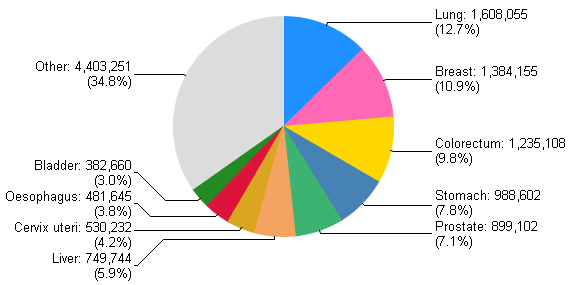
\includegraphics[width=.85\textwidth]{./images/statistics/repartitionCancerIncidence.png}
        \caption{\tiny \# cancer cases}
      \end{figure}
    \end{block}}
  \only<2>{
    \begin{block}{\small Statistics\footnotemark}
      \begin{figure}%
        \centering
        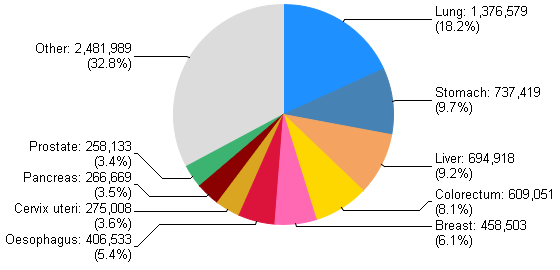
\includegraphics[width=.85\textwidth]{./images/statistics/repartitionCancerDeaths.png}
        \caption{\tiny \# cancer deaths}
      \end{figure}
    \end{block}}
  \footcitetext{Ferlay2010}
\end{frame}

\subsection{The prostate organ}

\begin{frame}
  \frametitle{Introduction}
  \framesubtitle{The prostate organ}
  \begin{block}{\small Anatomy}
    \begin{figure}%
      \centering
      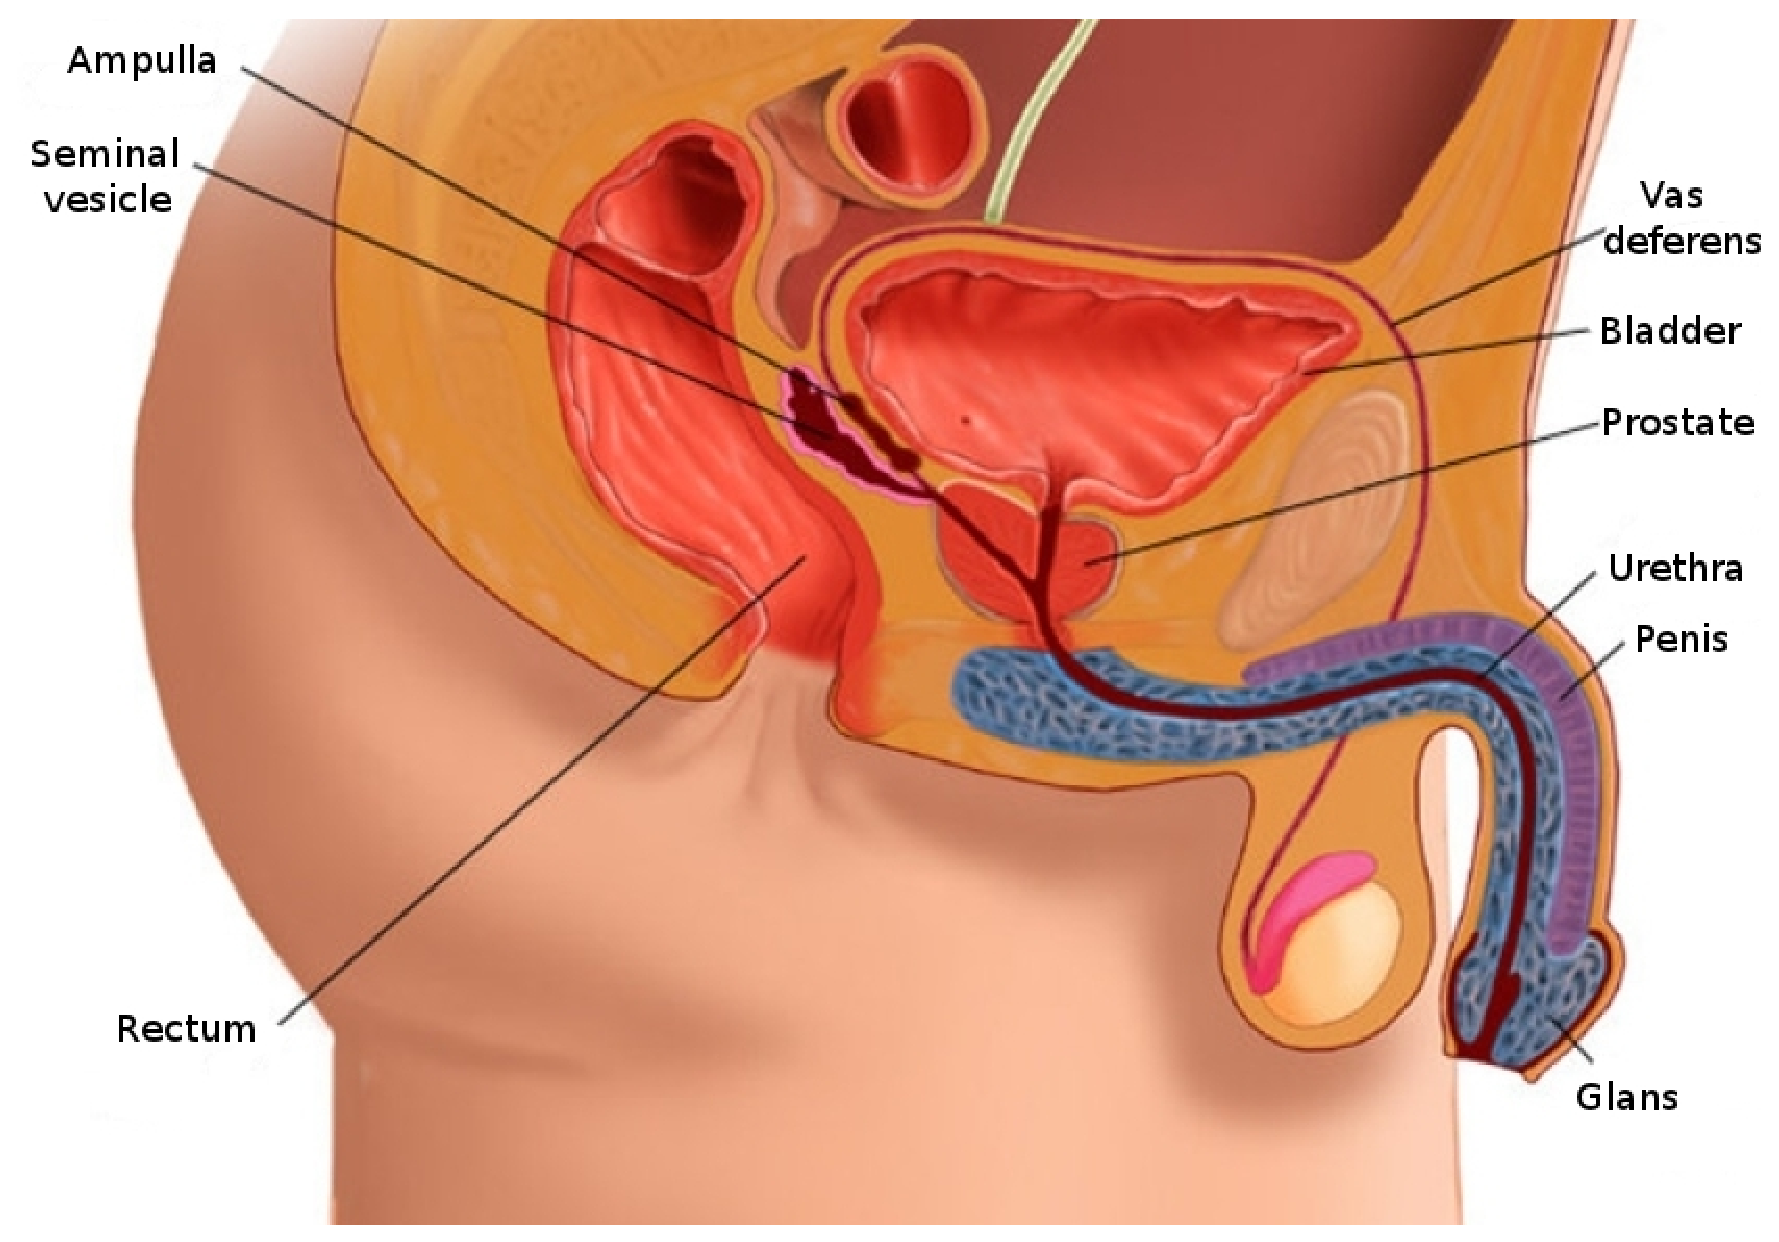
\includegraphics[height=.3\textheight]{./images/anatomy/prostate2D.eps}
      \caption{\tiny Localization of the prostate organ, image source\footnotemark}
    \end{figure}
  \end{block}
  \begin{block}{\small Characteristics}\scriptsize
    \begin{itemize}
    \item Height: \SI{3}{\cm}
    \item Depth: \SI{2.5}{\cm}
    \item Weight: \SIrange{7}{16}{\g}
    \end{itemize}
  \end{block}
  \footcitetext{Geckomedia2011}
\end{frame}

\setcounter{subfigure}{0}% Reset subfigure counter

\begin{frame}
  \frametitle{Introduction}
  \framesubtitle{The prostate organ}
  \begin{block}{\small Anatomy}
    \begin{figure}%
      \centering
      \hspace*{\fill}%
      \subfigure[][\tiny Transverse plane]{%
        \label{fig:stat1a}%
        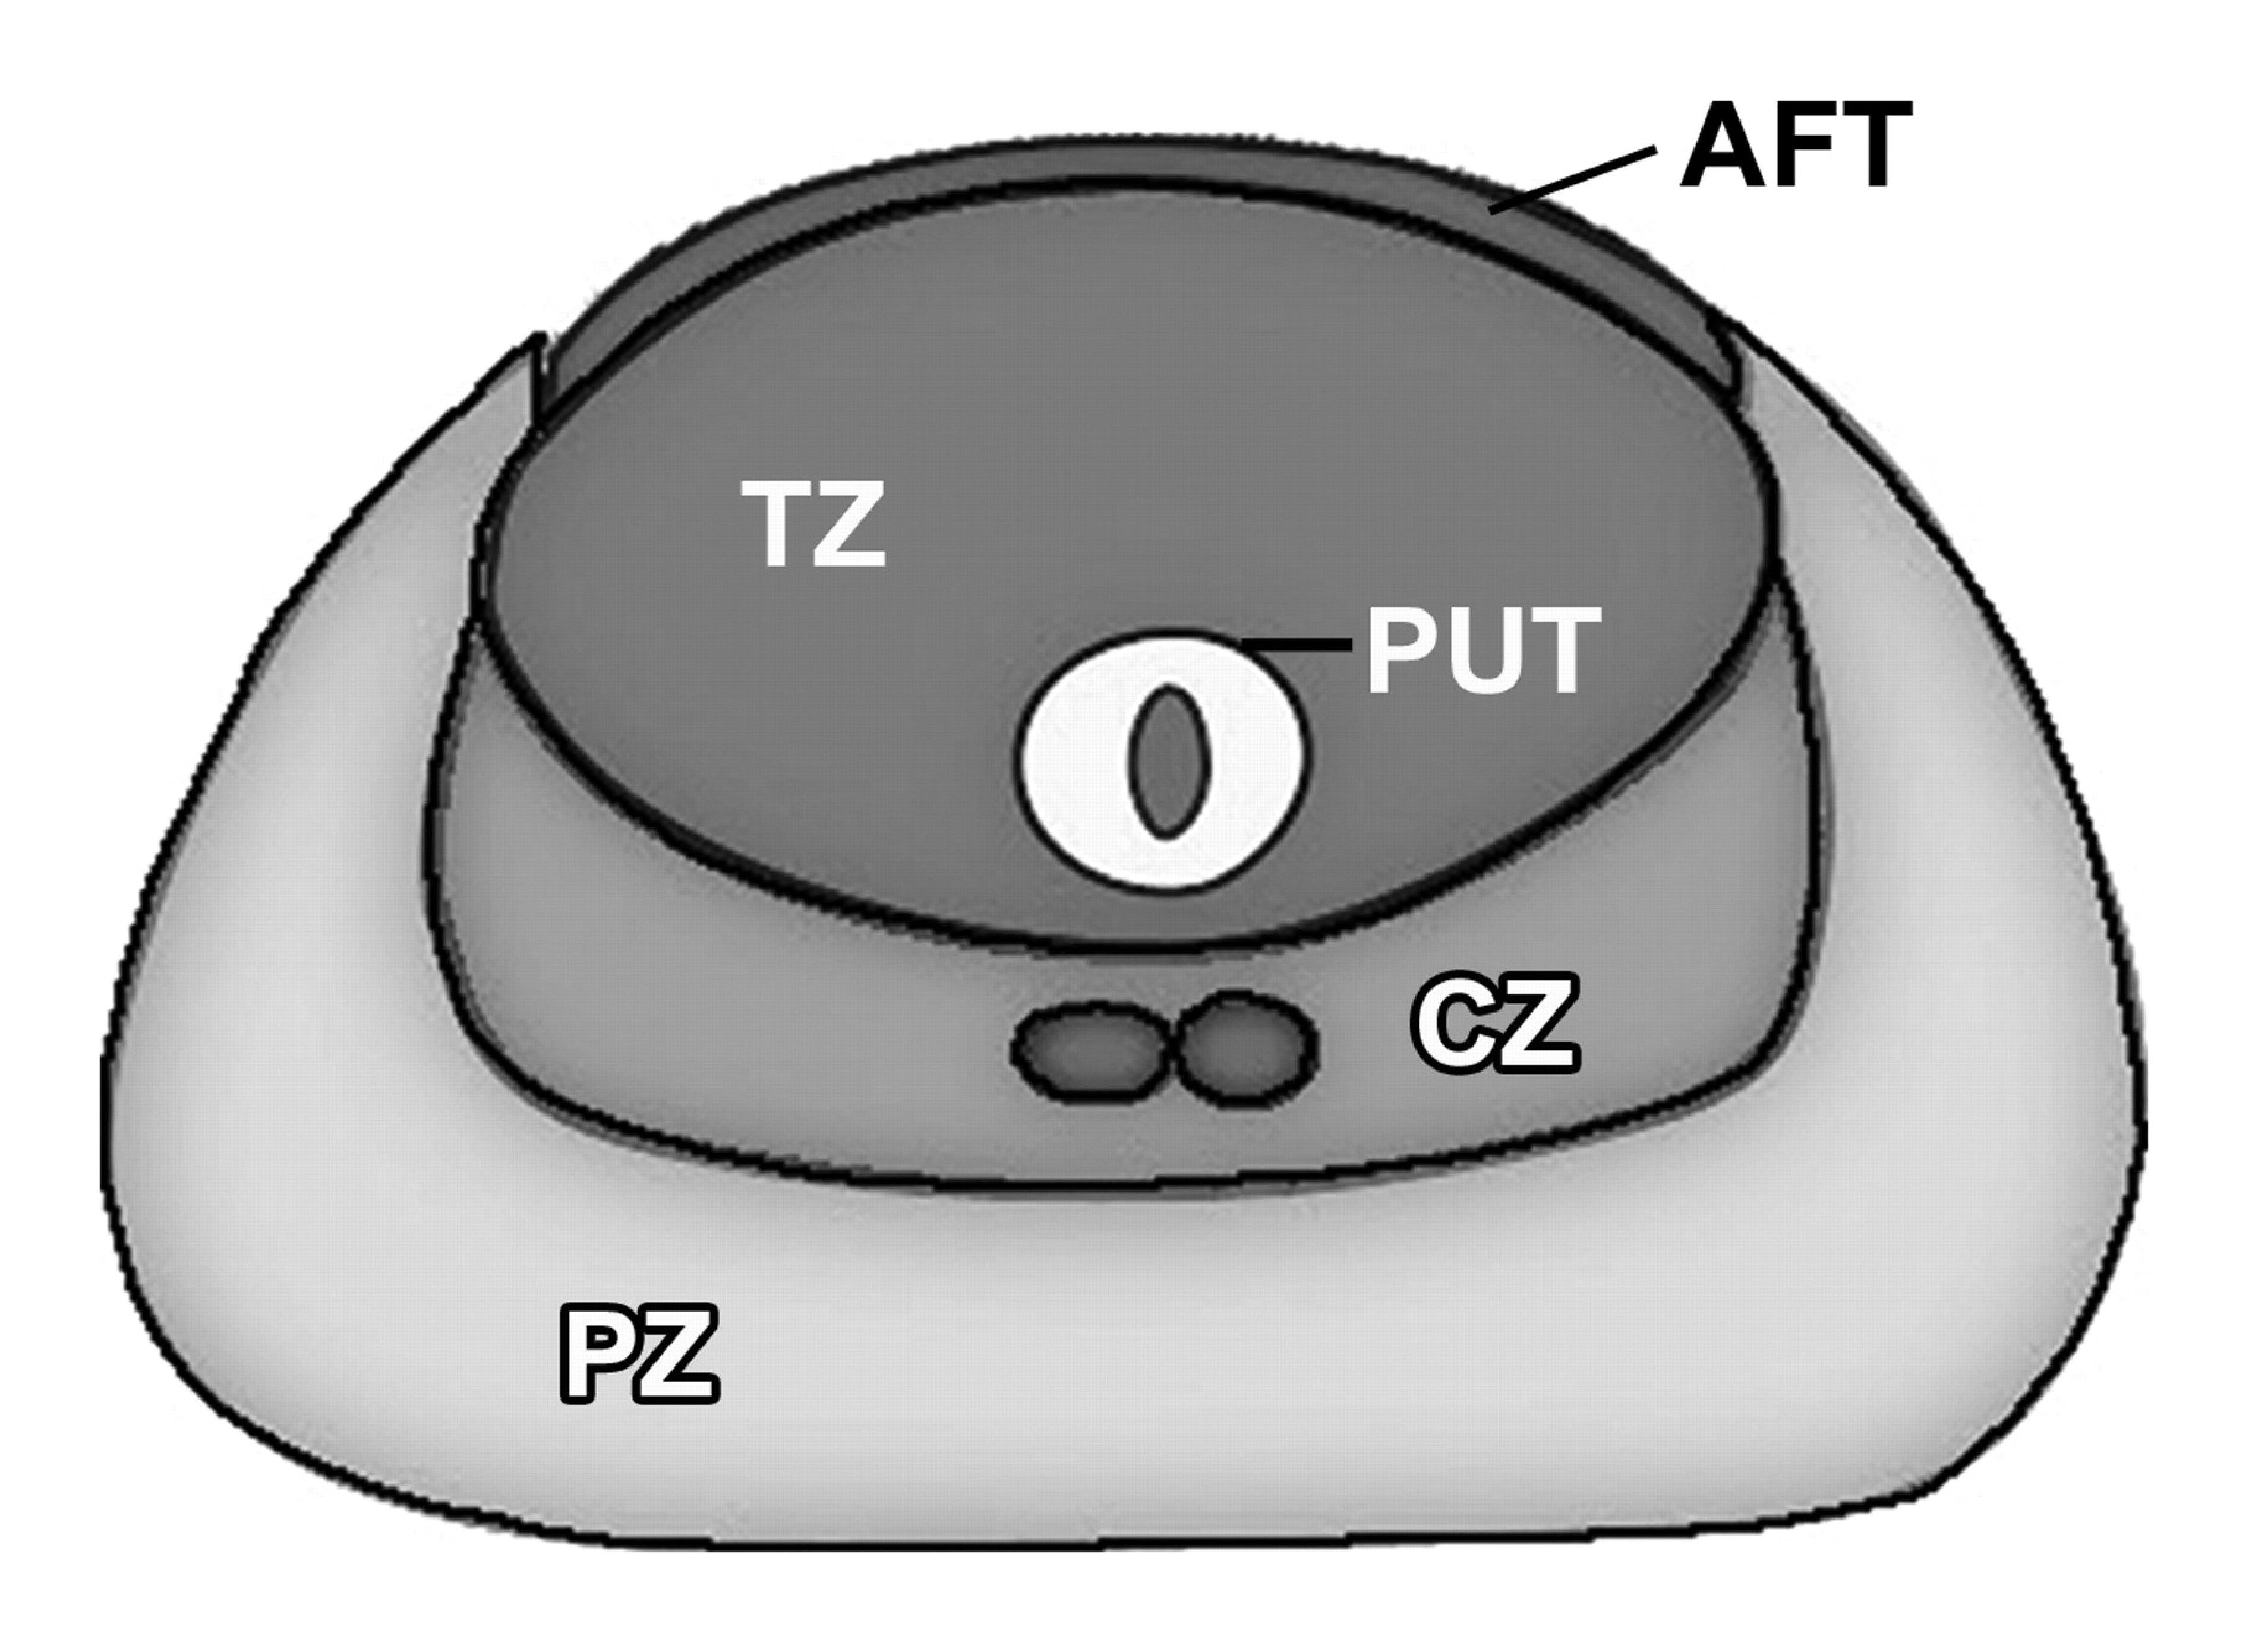
\includegraphics[height=.28\textheight]{./images/anatomy/prostateTransverse.eps}}%
      \hfill%
      \subfigure[][\tiny Sagittal plane]{%
        \label{fig:stat1b}%
        \includegraphics[height=.35\textheight]{./images/anatomy/prostateSagital.eps}}%
      \hspace*{\fill}%
      \caption{\tiny Prostate zones - AFT: anterior fibromuscular tissue, CZ: central zone, ED: ejaculatory duct, NVB: neurovascular bundle, PUT: periurethral tissue, PZ: peripheral zone, U: urethra, TZ: transitional zone, B: base, M: median, A: apex; image source\footnotemark}
      \label{fig:stat1}%
    \end{figure}
  \end{block}
  \footcitetext{Choi2007}
\end{frame}

\subsection{Prostate carcinoma}

\begin{frame}
  \frametitle{Introduction}
  \framesubtitle{Prostate carcinoma (CaP)}
  \begin{center}
    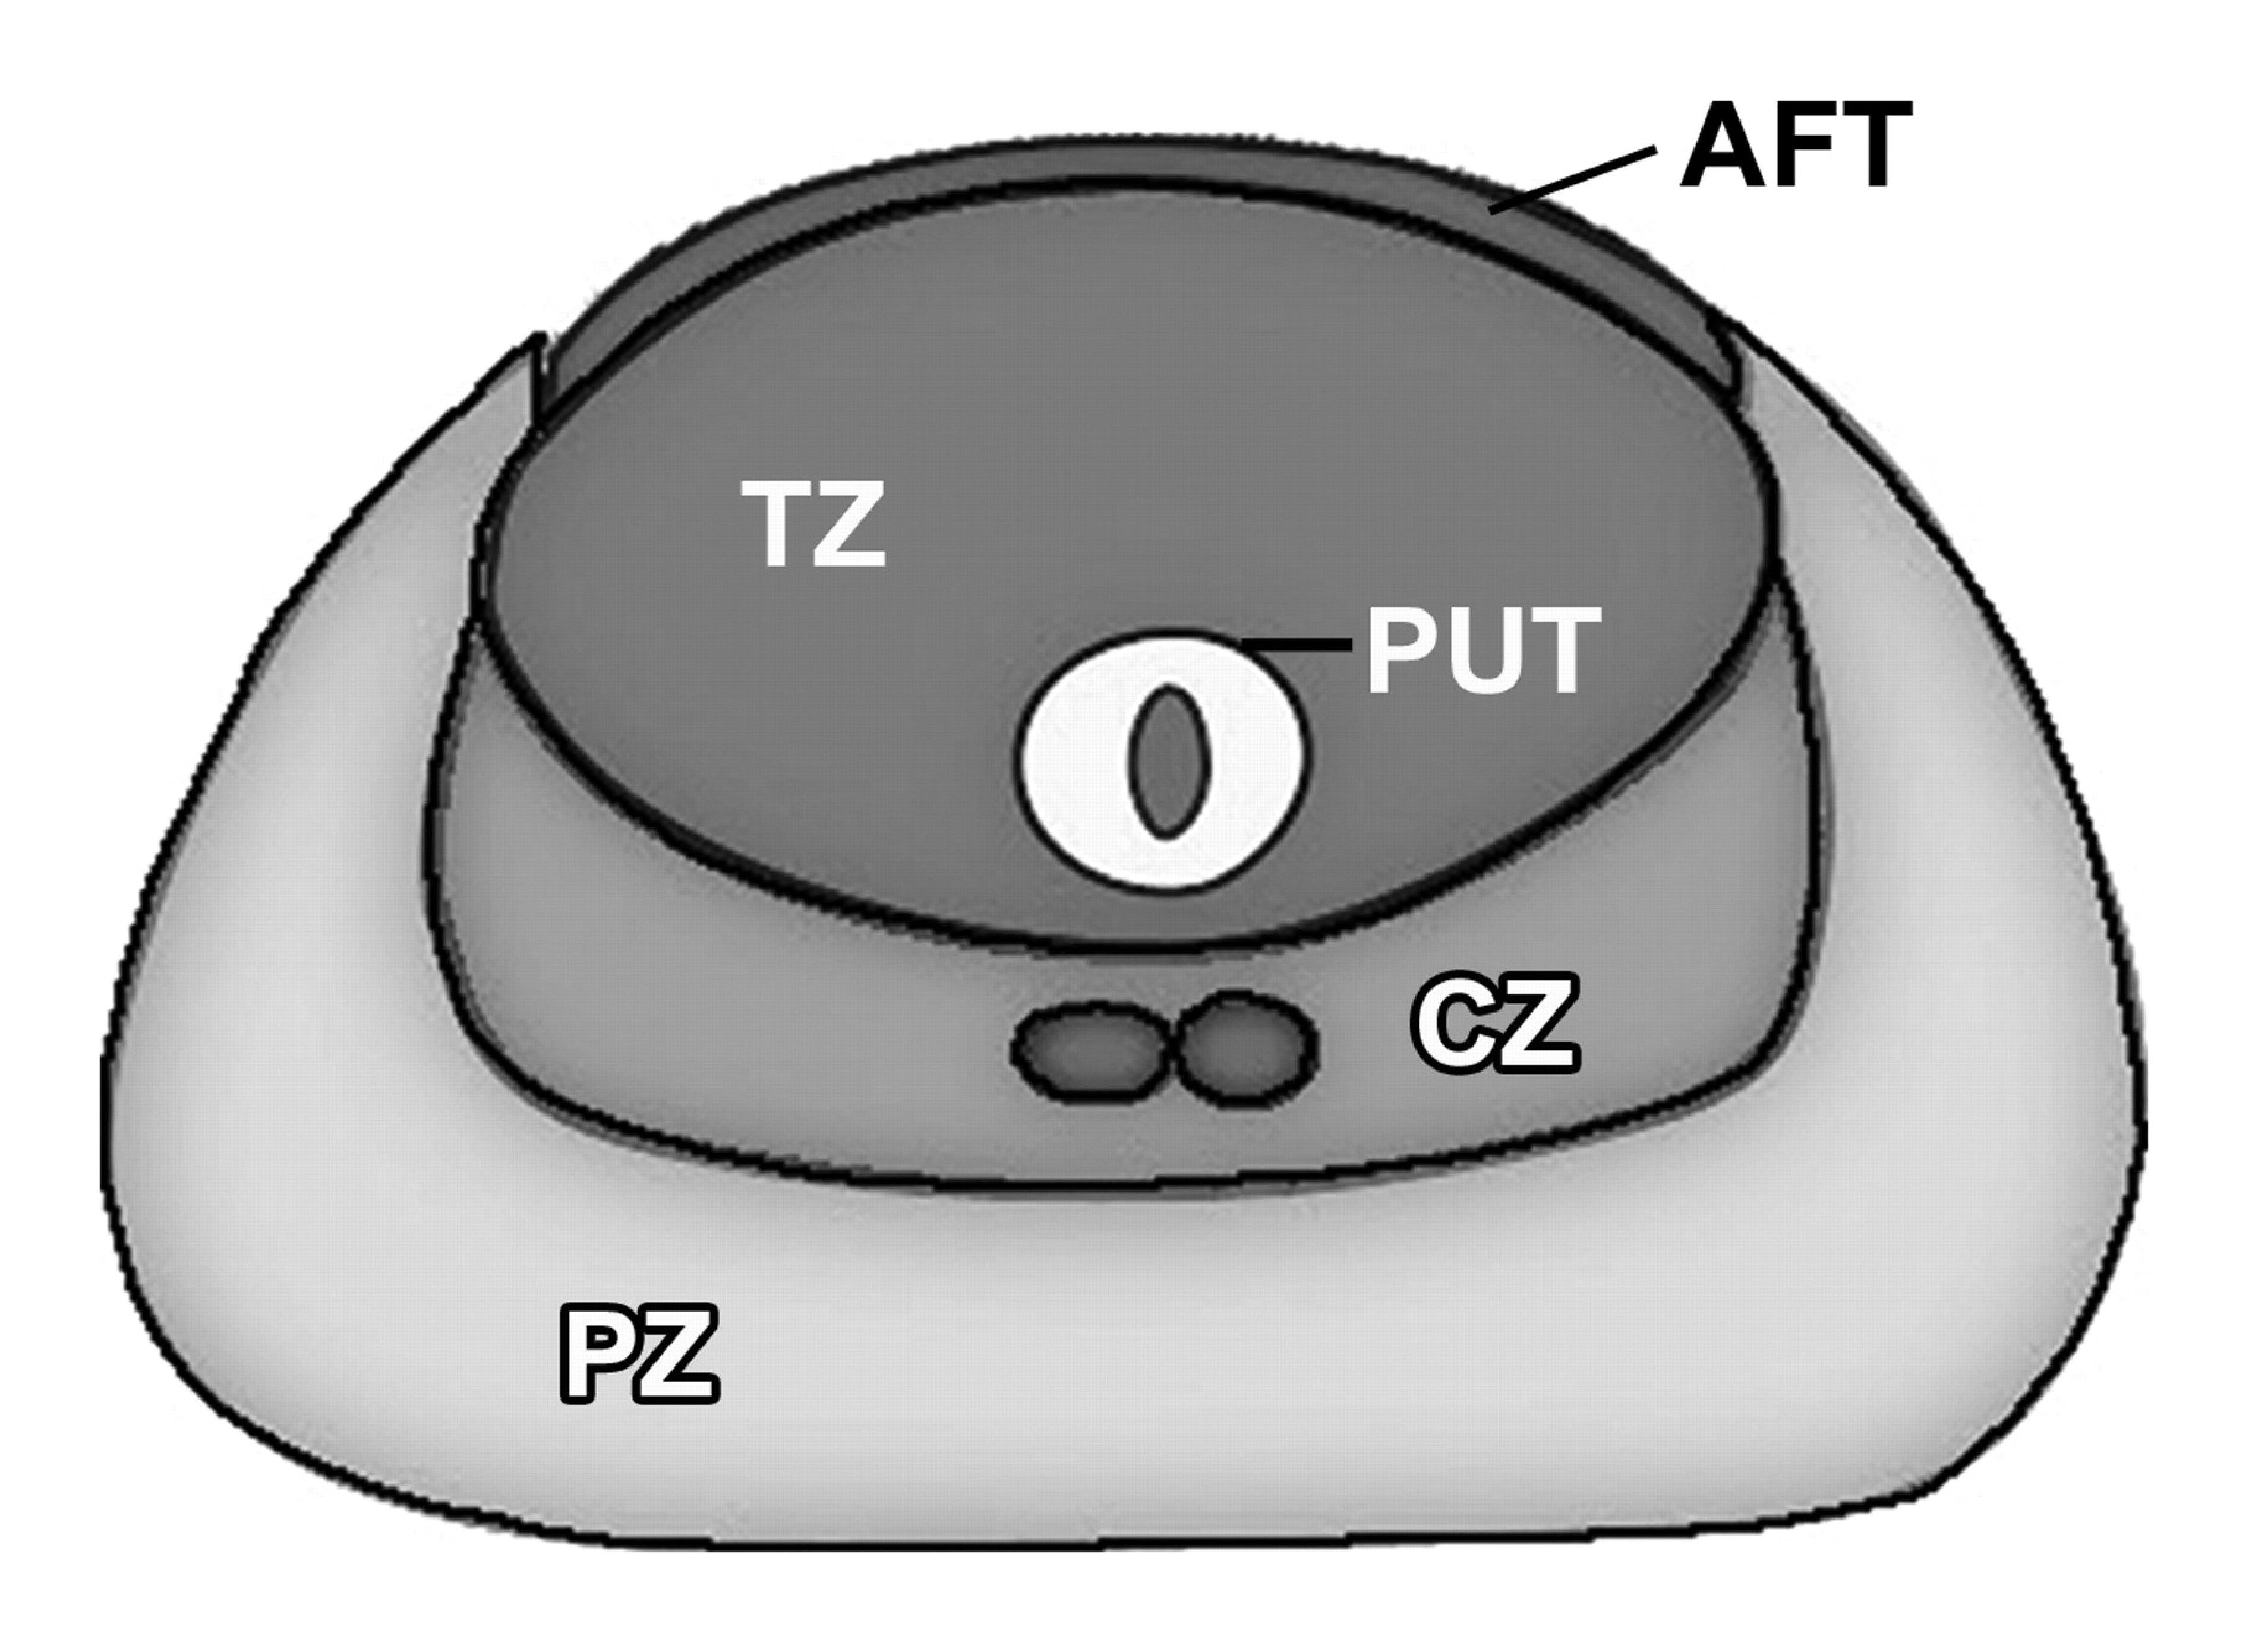
\includegraphics[height=.25\textheight]{./images/anatomy/prostateTransverse.eps}
  \end{center}
  \begin{columns}
    \begin{column}{0.45\textwidth}
      \begin{block}{\small CaP development}
        \begin{itemize}\scriptsize
        \item Slow-growing $\rightarrow$ \SI{85}{\percent}
        \item Fast-growing $\rightarrow$ \SI{15}{\percent}
        \item CaPs in CG (TZ+CZ) are more aggressive
        \end{itemize}
      \end{block}
    \end{column}
    \begin{column}{0.45\textwidth}
      \begin{block}{\small Zonal predisposition}
        \begin{itemize}\scriptsize
        \item PZ $\rightarrow$ \SIrange{70}{80}{\percent}
        \item TZ $\rightarrow$ \SIrange{10}{20}{\percent}
        \item CZ $\rightarrow$ \SI{5}{\percent}
        \end{itemize}
      \end{block}
    \end{column}
  \end{columns}
  \begin{greenblock}{\small What clinicians need?}
    \begin{itemize}\scriptsize
    \item Detect CaP
    \item Distinguish slow- from fast-growing CaP
    \item Active surveillance \emph{vs.} prostatectomy/other treatments
    \end{itemize}
  \end{greenblock}
\end{frame}

\subsection{Screening}

\begin{frame}
  \frametitle{Introduction}
  \framesubtitle{Screening}
  \begin{columns}
    \begin{column}{0.5\textwidth}
      \begin{block}<1->{\small Prostate-specific antigen}
        \begin{itemize}\scriptsize
        \item<1-> $>$ \SI{10}{\nano\gram\per\milli\liter} $\rightarrow$ biopsy
        \item<2-> From \SIrange{4}{10}{\nano\gram\per\milli\liter}
          \begin{itemize}\scriptsize
          \item[$\rightarrow$] $\frac{\text{\tikzbullet{gray}{orangeubfc}}}{\text{\tikzbullet{gray}{orangeubfc}}\  +\  \text{\tikzbullet{gray}{blueubfc}}} > 15 \% \rightarrow$ biopsy
          \end{itemize}
        %\item[\cross]<3-> Not reliable
        \end{itemize}
      \end{block}
      \begin{block}<1->{\small ``Blind'' transrectal ultrasound biopsy}
        \begin{itemize}\scriptsize
        \item<3-> Take samples from different locations
        \item<3-> Grade using Gleason score
        %\item[\cross]<5-> Invasive procedure
        %\item[\cross]<5-> Lead to false positives \& negatives
        \end{itemize}
      \end{block}
    \end{column}
    \begin{column}{0.5\textwidth}
      \begin{center}
        \only<1>{
          \begin{figure}
            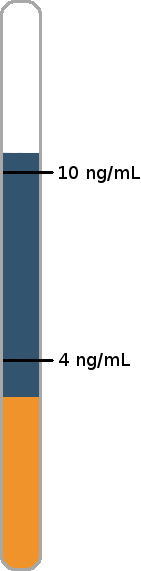
\includegraphics[height=.6\textheight]{./images/screening/high_psa.png}
            \caption{\tiny \tikzbullet{gray}{orangeubfc} free PSA \\ \tikzbullet{gray}{blueubfc} protein-linked PSA}
          \end{figure}
        }
        \only<2>{
          \begin{figure}
            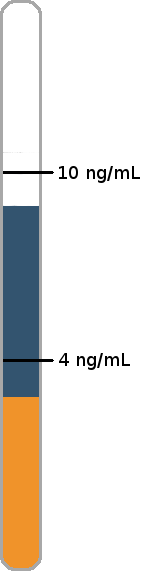
\includegraphics[height=.6\textheight]{./images/screening/risk_psa.png}
            \caption{\tiny \tikzbullet{gray}{orangeubfc} free PSA \\ \tikzbullet{gray}{blueubfc} protein-linked PSA}
          \end{figure}
        }
        % \only<3>{
        %   \begin{figure}
        %     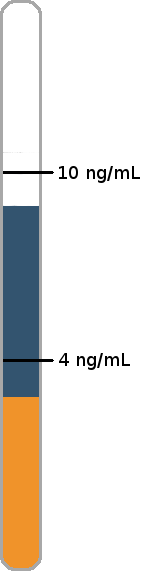
\includegraphics[height=.6\textheight]{./images/screening/risk_psa.png}
        %     \caption{\tiny \tikzbullet{gray}{orangeubfc} free PSA \\ \tikzbullet{gray}{blueubfc} protein-linked PSA}
        %   \end{figure}
        % }
        \only<3>{
          \begin{figure}
            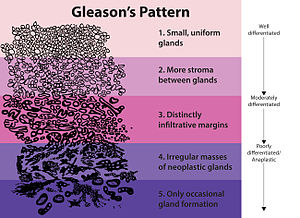
\includegraphics[height=.45\textheight]{./images/screening/gleason.jpg}
            \caption{\tiny Image source: \texttt{https://goo.gl/fEVQXQ}}
          \end{figure}
        }
        % \only<4>{
        %   \begin{figure}
        %     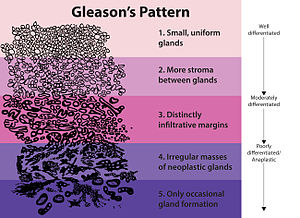
\includegraphics[height=.4\textheight]{./images/screening/gleason.jpg}
        %     \caption{\tiny Image source: \texttt{https://goo.gl/fEVQXQ}}
        %   \end{figure}
        % }
        % \only<6>{
        %   \begin{greenblock}{\small Pros}
        %     \begin{itemize}\scriptsize
        %     \item[\tick]<6-> Reduce CaP-related mortality from \SIrange{21}{44}{\percent}\footnotemark
        %     \end{itemize}
        %   \end{greenblock}
        %   \begin{redblock}{\small Cons}
        %     \begin{itemize}\scriptsize
        %     \item[\cross] Up to \SI{30}{\percent} of over-diagnosis\footnotemark
        %     \item[\cross] Up to \SI{35}{\percent} of undiagnosed CaP\footnotemark
        %     \item[\cross] Biopsies are invasive
        %     \end{itemize}
        %   \end{redblock}}
      \end{center}
     \end{column}
     %\only<6>{\addtocounter{footnote}{-3} \stepcounter{footnote} \footcitetext{Schroeder2012} \stepcounter{footnote} \footcitetext{Haas2007} \stepcounter{footnote} \footcitetext{Taira2010}}
   \end{columns}
\end{frame}

\begin{frame}
  \frametitle{Introduction}
  \framesubtitle{Screening}
  \begin{greenblock}{\small Pros}
    \begin{itemize}\scriptsize
    \item[\tick] Reduce CaP-related mortality between \SI{21}{\percent} and \SI{44}{\percent}\footnotemark
    \end{itemize}
  \end{greenblock}
  \begin{redblock}{\small Cons}
    \begin{itemize}\scriptsize
    \item[\cross] Up to \SI{30}{\percent} of over-diagnosis\footnotemark
    \item[\cross] Up to \SI{35}{\percent} of undiagnosed CaP\footnotemark
    \item[\cross] Biopsies are invasive
    \end{itemize}
  \end{redblock}
  \addtocounter{footnote}{-3} \stepcounter{footnote} \footcitetext{Schroeder2012} \stepcounter{footnote} \footcitetext{Haas2007} \stepcounter{footnote} \footcitetext{Taira2010}
\end{frame}

\subsection{CAD and mp-MRI}

\begin{frame}
  \frametitle{Introduction}
  \framesubtitle{CAD and mp-MRI}
  \begin{greenblock}{\small Current trendy techniques: mp-MRI}
    \begin{itemize}\scriptsize
    \item[\tick] Less invasive technique
    \end{itemize}
  \end{greenblock}
  \begin{redblock}{\small Human diagnosis using mp-MRI}
    \begin{itemize}\scriptsize
    \item[\cross] Need further investigation of the mp-MRI modalities
    \item[\cross] Low repeatability
      \begin{itemize} \scriptsize
      \item Observer limitations
      \item Complexity of clinical cases
      \end{itemize}
    \end{itemize}
  \end{redblock}
  \begin{block}{\small Emergence of CAD}
    \begin{itemize}\scriptsize
    \item CADe $\rightarrow$ detection of potential lesions
    \item CADx $\rightarrow$ diagnosis regarding those lesions
    \end{itemize}
  \end{block}
\end{frame}

\subsection{Research objectives}

\begin{frame}
  \frametitle{Introduction}
  \framesubtitle{Research objectives}
  \begin{block}{\small Propose a mp-MRI CAD for CaP}
    \begin{itemize}\scriptsize
    \item Study and investigate the state-of-the-art on mp-MRI CAD for CaP
    \item Identify the scientific barriers
    \item Design a mp-MRI CAD addressing these issues
    \item Investigate and analyze the proposed CAD
    \end{itemize}
  \end{block}
\end{frame}

\section{State-of-the-art}

\begin{frame}
  \begin{scriptsize}
    \tableofcontents[currentsection,currentsubsection,subsectionstyle=show/show/hide]
  \end{scriptsize}
\end{frame}

\subsection{MRI modalities}

\setcounter{subfigure}{0}% Reset subfigure counterw

\begin{frame}
  \frametitle{Introduction}
  \framesubtitle{MRI modalities}
  \begin{block}{\small T$_2$W-MRI}
    \begin{figure}%
      \centering
      \hspace*{\fill}%
      \subfigure[][\tiny Healthy]{%
        \label{fig:t2wh}%
        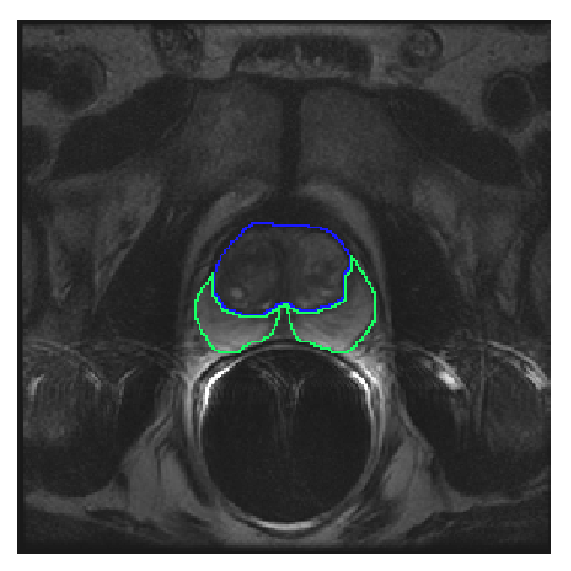
\includegraphics[width=.2\textwidth]{./images/mri/t2w/t2w_healthy.eps}}%
      \hfill%
      \subfigure[][\tiny CaP PZ]{%
        \label{fig:t2wcpz}%
        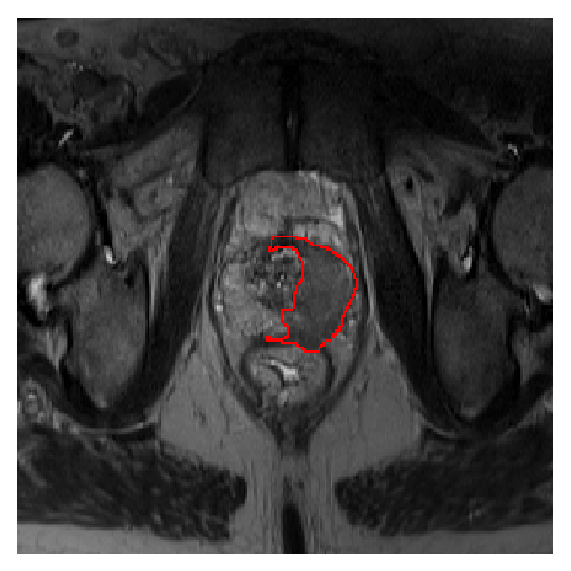
\includegraphics[width=.2\textwidth]{./images/mri/t2w/t2w_cancer_pz.eps}}%
      \hfill%
      \subfigure[][\tiny CaP CG]{%
        \label{fig:t2wccg}%
        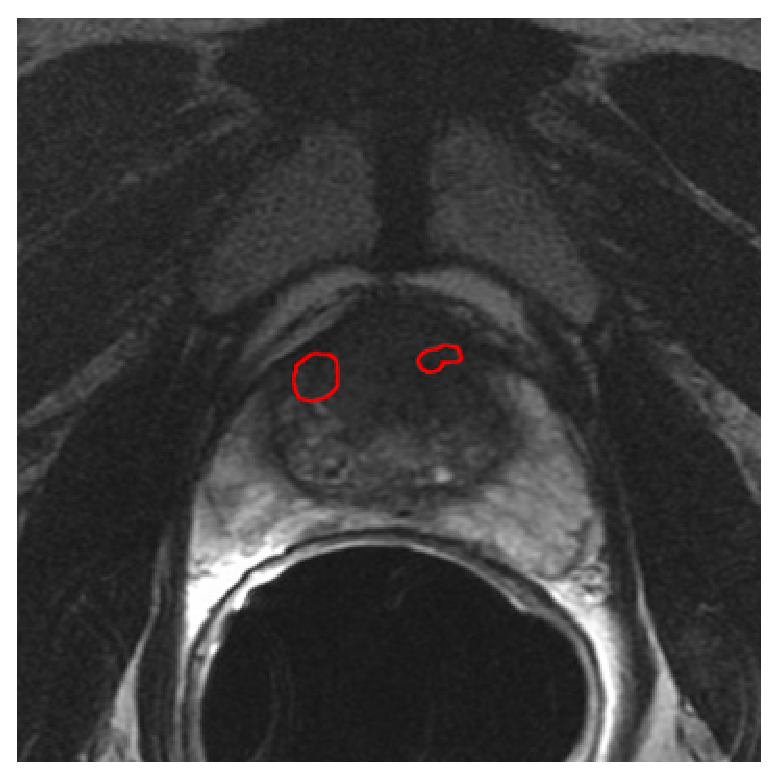
\includegraphics[width=.2\textwidth]{./images/mri/t2w/t2w_cancer_cg.eps}}%
      \hspace*{\fill}%
      \label{fig:t2w}%
    \end{figure}
  \end{block}
  \begin{columns}
    \begin{column}{0.5\textwidth}
      \begin{block}{\small Healthy \emph{vs.} CaP}\footnotesize
        \begin{itemize}\scriptsize
        \item Lower SI
        \item Ill-defined edges
        \end{itemize}
      \end{block}
    \end{column}
    \begin{column}{0.5\textwidth}
      \begin{block}{\small Pros and cons}\footnotesize
        \begin{itemize}\scriptsize
        \item[\tick] High resolution
        \item[\tick] Anatomy well depicted
        \item[\cross] Low sensitivity in CG
        \item[\cross] Lower specificity due to outliers
        \end{itemize}
      \end{block}
    \end{column}
  \end{columns}
  % \only<1>{
  %   \begin{columns}
  %     \begin{column}{0.5\textwidth}
  %       \begin{greenblock}{\small Healthy}\footnotesize
  %         \begin{itemize}\scriptsize
  %         \item Intermediate to high-signal intensity (SI) in PZ
  %         \item Low-SI in CG
  %         \end{itemize}
  %       \end{greenblock}
  %     \end{column}
  %     \begin{column}{0.5\textwidth}
  %       \begin{redblock}{\small CaP}\footnotesize
  %         \begin{itemize}\scriptsize
  %         \item Low-SI
  %         \item Round and ill-defined mass in PZ
  %         \item Homogeneous with ill-defined edges in CG
  %         \end{itemize}
  %       \end{redblock}
  %     \end{column}
  %   \end{columns}}
  % \setcounter{subfigure}{0}% Reset subfigure counter
  % \only<2>{
  %   \begin{columns}
  %     \begin{column}{0.5\textwidth}
  %       \begin{greenblock}{\small Pros}\footnotesize
  %         \begin{itemize}\scriptsize
  %         \item Highest spatial resolution
  %         \item Anatomy nicely depicted
  %         \end{itemize}
  %       \end{greenblock}
  %     \end{column}
  %     \begin{column}{0.5\textwidth}
  %       \begin{redblock}{\small Cons}\footnotesize
  %         \begin{itemize}\scriptsize
  %         \item Low sensitivity in CG
  %         \item Lower specificity due to outliers
  %         \end{itemize}
  %       \end{redblock}
  %     \end{column}
  %   \end{columns}}
\end{frame}

\setcounter{subfigure}{0}% Reset subfigure counter

\begin{frame}
  \frametitle{Introduction}
  \framesubtitle{MRI modalities}
  \begin{block}{\small DCE-MRI}
    \begin{figure}%
      \centering
      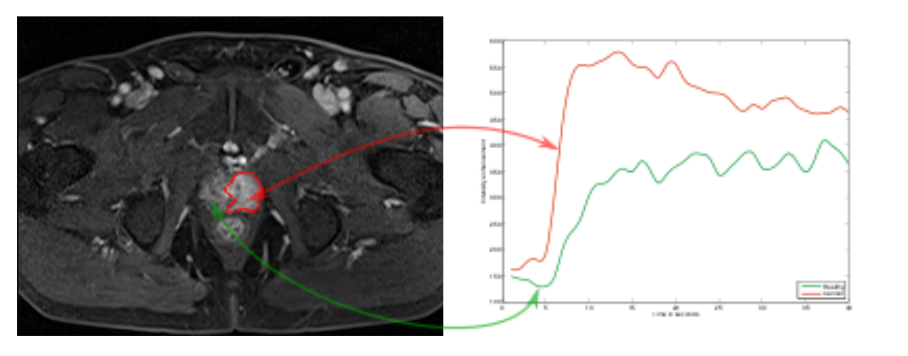
\includegraphics[width=.63\textwidth]{./images/mri/dce/dce_cancer_healthy_information.eps}
      \label{fig:dce}%
      \caption{\tiny {\color{green}Green}: healthy - {\color{red}Red}: CaP}
    \end{figure}
  \end{block}
  \begin{columns}
    \begin{column}{0.5\textwidth}
      \begin{block}{\small Healthy \emph{vs.} CaP}\footnotesize
        \begin{itemize}\scriptsize
        \item Faster wash-in, wash-out, time-to-peak enhancement
        \item Higher integral under the curve, max SI
        \end{itemize}
      \end{block}
    \end{column}
    \begin{column}{0.5\textwidth}
      \begin{block}{\small Pros and cons}\footnotesize
        \begin{itemize}\scriptsize
        \item[\tick] Information about vascularity
        \item[\cross] Spatial mis-registration
        \item[\cross] Lower spatial resolution
        \item[\cross] Difficult detection in CG
        \item[\cross] Curve variations among patients
        \end{itemize}
      \end{block}
    \end{column}
  \end{columns}
%   \only<1>{
%     \begin{columns}
%       \begin{column}{0.5\textwidth}
%         \begin{greenblock}{\small Healthy}
%           \begin{itemize}\scriptsize
%           \item Slower wash-in, wash-out, time-to-peak enhancement
%           \item Lower integral under the curve, max SI
%           \end{itemize}
%         \end{greenblock}
%       \end{column}
%       \begin{column}{0.5\textwidth}
%         \begin{redblock}{\small CaP}
%           \begin{itemize}\scriptsize
%           \item Faster wash-in, wash-out, time-to-peak enhancement
%           \item Higher integral under the curve, max SI
%           \end{itemize}
%         \end{redblock}
%       \end{column}
%     \end{columns}}
% \setcounter{subfigure}{0}% Reset subfigure counter
%   \only<2>{
%     \begin{columns}
%       \begin{column}{0.5\textwidth}
%         \begin{greenblock}{\small Pros}\footnotesize
%           \begin{itemize}\scriptsize
%           \item Information about vascularity
%           \end{itemize}
%         \end{greenblock}
%       \end{column}
%       \begin{column}{0.5\textwidth}
%         \begin{redblock}{\small Cons}\footnotesize
%           \begin{itemize}\scriptsize
%           \item Spatial mis-registration
%           \item Lower spatial resolution than T$_2$W-MRI
%           \item Difficult detection in CG
%           \end{itemize}
%         \end{redblock}
%       \end{column}
%     \end{columns}}
\end{frame}

\setcounter{subfigure}{0}% Reset subfigure counter

\begin{frame}
  \frametitle{Introduction}
  \framesubtitle{MRI modalities}
  \begin{block}{\small DW-MRI - ADC}
    \begin{figure}%
      \centering
      \hspace*{\fill}%
      \subfigure[][\tiny DW MRI]{%
        \label{fig:dw}%
        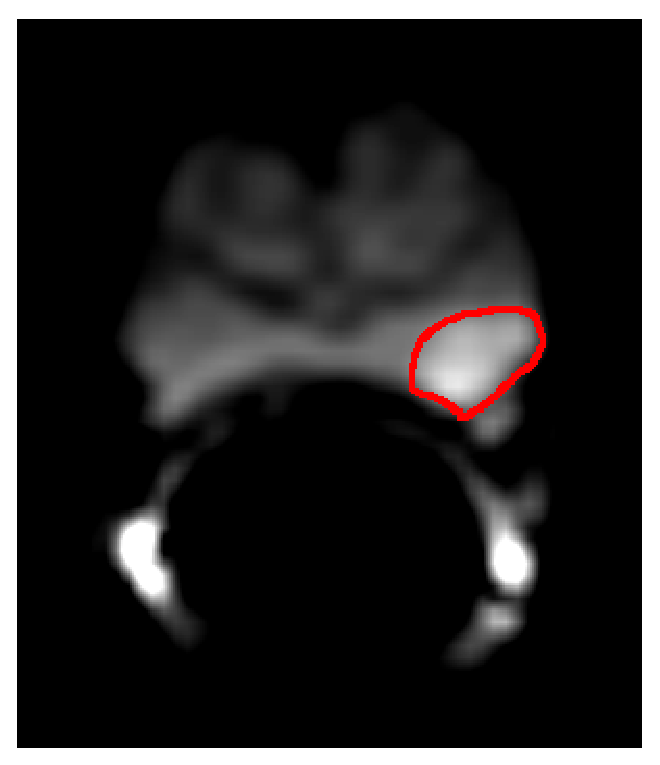
\includegraphics[width=.2\textwidth]{./images/mri/dwi/dwi_cancer.eps}}%
      \hfill%
      \subfigure[][\tiny ADC]{%
        \label{fig:adc}%
        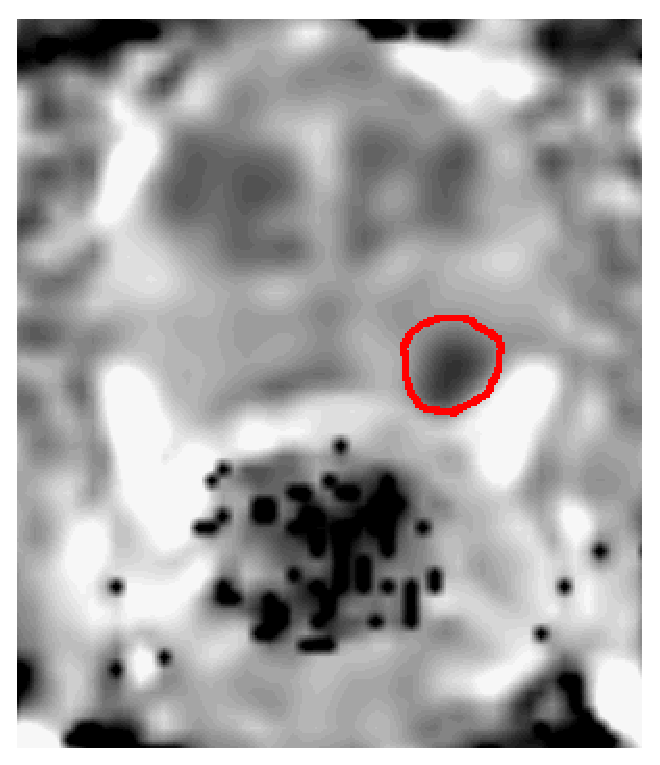
\includegraphics[width=.2\textwidth]{./images/mri/dwi/adc_cancer.eps}}%
      \hspace*{\fill}%
      \label{fig:dwadc}%
    \end{figure}
  \end{block}
  \begin{columns}
    \begin{column}{0.5\textwidth}
      \begin{block}{\small Healthy \emph{vs.} CaP}\footnotesize
        \begin{itemize}\scriptsize
        \item DW-MRI: higher SI
        \item ADC: lower SI
        \end{itemize}
      \end{block}
    \end{column}
    \begin{column}{0.5\textwidth}
      \begin{block}{\small Pros and cons}\footnotesize
        \begin{itemize}\scriptsize
        \item[\tick] Information about tissue structure
        \item[\tick] ADC correlated with Gleason score
        \item[\cross] Poor spatial resolution
        \item[\cross] Variability of the ADC coefficient
        \end{itemize}
      \end{block}
    \end{column}
  \end{columns}
%   \only<1>{
%     \begin{columns}
%       \begin{column}{0.5\textwidth}
%         \begin{greenblock}{\small Healthy}
%           \begin{itemize}\scriptsize
%           \item DW-MRI: lower SI
%           \item ADC: higher-SI
%           \end{itemize}
%         \end{greenblock}
%       \end{column}
%       \begin{column}{0.5\textwidth}
%         \begin{redblock}{\small CaP}\scriptsize
%           \begin{itemize}
%           \item DW-MRI: higher SI
%           \item ADC: lower-SI
%           \end{itemize}
%         \end{redblock}
%       \end{column}
%     \end{columns}}
% \setcounter{subfigure}{0}% Reset subfigure counter
%   \only<2>{
%     \begin{columns}
%       \begin{column}{0.5\textwidth}
%         \begin{greenblock}{\small Pros}
%           \begin{itemize}\scriptsize
%           \item Information about tissue structure
%           \item ADC correlated with Gleason score
%           \end{itemize}
%         \end{greenblock}
%       \end{column}
%       \begin{column}{0.5\textwidth}
%         \begin{redblock}{\small Cons}\scriptsize
%           \begin{itemize}
%           \item Poor spatial resolution
%           \item Variability of the ADC coefficient
%           \end{itemize}
%         \end{redblock}
%       \end{column}
%     \end{columns}}
\end{frame}

\setcounter{subfigure}{0}% Reset subfigure counter

\begin{frame}
  \frametitle{Introduction}
  \framesubtitle{MRI modalities}
  \begin{block}{\small MRSI}
    \begin{figure}%
      \centering
      \hspace*{\fill}%
      \subfigure[][\tiny Healthy]{%
        \label{fig:mrsih}%
        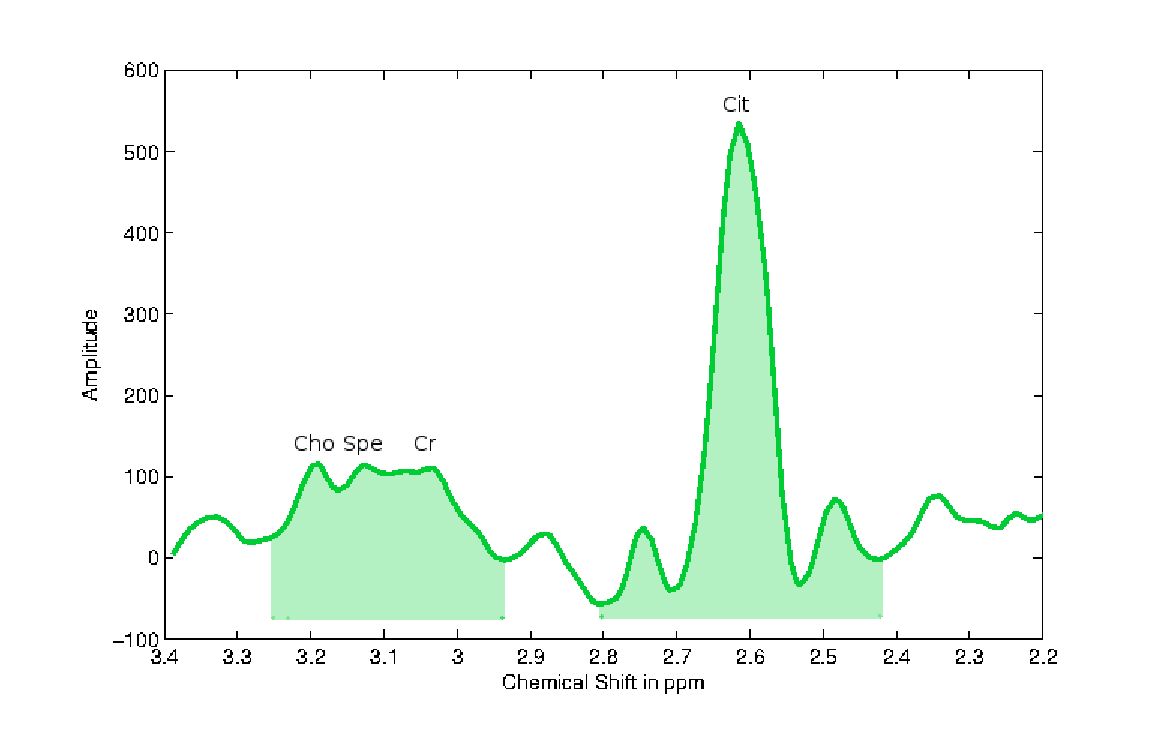
\includegraphics[width=.45\textwidth]{./images/mri/mrsi/mrsi_healthy.eps}}%
      \hfill%
      \subfigure[][\tiny CaP]{%
        \label{fig:mrsic}%
        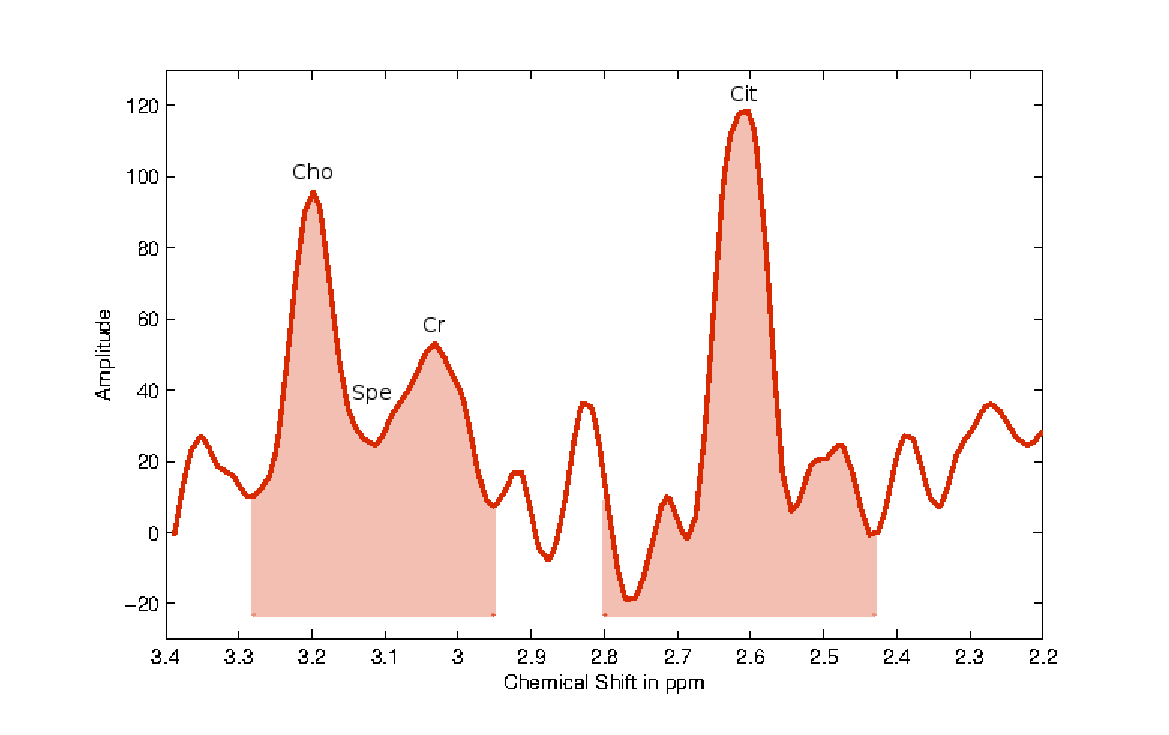
\includegraphics[width=.45\textwidth]{./images/mri/mrsi/mrsi_cancer.eps}}%
      \hspace*{\fill}%
      \label{fig:mrsi}%
    \end{figure}
  \end{block}
  \begin{columns}
    \begin{column}{0.5\textwidth}
      \begin{block}{\small Healthy \emph{vs.} CaP}\footnotesize
        \begin{itemize}\scriptsize
        \item Decrease of citrate and spermine concentrations
        \item Increase of choline concentration
        \end{itemize}
      \end{block}
    \end{column}
    \begin{column}{0.5\textwidth}
      \begin{block}{\small Pros and cons}\footnotesize
        \begin{itemize}\scriptsize
        \item[\tick] Citrate correlated with Gleason score
        \item[\cross] Low spatial resolution
        \item[\cross] Variation inter-patients
        \end{itemize}
      \end{block}
    \end{column}
  \end{columns}
%   \only<1>{
%     \begin{columns}
%       \begin{column}{0.5\textwidth}
%         \begin{greenblock}{\small Healthy}
%           \begin{itemize}\scriptsize
%           \item High citrate concentration
%           \item Moderate choline and spermine concentrations
%           \end{itemize}
%         \end{greenblock}
%       \end{column}
%       \begin{column}{0.5\textwidth}
%         \begin{redblock}{\small CaP}
%           \begin{itemize}\scriptsize
%           \item Decrease of citrate and spermine concentrations
%           \item Increase of choline concentration
%           \end{itemize}
%         \end{redblock}
%       \end{column}
%     \end{columns}}
% \setcounter{subfigure}{0}% Reset subfigure counter
%   \only<2>{
%     \begin{columns}
%       \begin{column}{0.5\textwidth}
%         \begin{greenblock}{\small Pros}\footnotesize
%           \begin{itemize}\scriptsize
%           \item Citrate correlated with Gleason score
%           \end{itemize}
%         \end{greenblock}
%       \end{column}
%       \begin{column}{0.5\textwidth}
%         \begin{redblock}{\small Cons}\footnotesize
%           \begin{itemize}\scriptsize
%           \item Low spatial resolution
%           \item Variation inter-patients
%           \end{itemize}
%         \end{redblock}
%       \end{column}
%     \end{columns}}
\end{frame}

\subsection{CAD for CaP}

%% \begin{frame}
%%   \frametitle{State-of-the-art}
%%   \framesubtitle{CAD for CaP}
%%   \begin{block}{\small block}
%%     \setcounter{subfigure}{0}% Reset subfigure counter

\begin{figure}%
  \hspace*{\fill}%
  \begin{tikzpicture}[scale=0.38, every node/.style={scale=0.38}]
    \piechartthreed[scale=0.8,
    mix color= darkgray]
    {120/orangeubfc,112/azulunam,120/greenubfc,8/purpleubfc}
    % \foreach \i in {1,...,3} { \fill (pc \i) circle (.5mm);}
    % \draw[darkgray] (pc 1) -- ++(0.4,0.8) node[anchor=south west] {CAD systems 60\%} coordinate (s1) -- ++(1,0);
    % \draw[darkgray] (pc 2) -- ++(-0.4,2.5) node[anchor=south west] at ++(0.2,0) {Features 7\%} coordinate (s1) -- ++(1,0);
    % \draw[darkgray] (pc 3) -- ++(0,0) node[anchor=south west] at ++(0.2,0) {Imaging 33\%} coordinate (s1) -- ++(1,0);
    % \draw[darkgray] (pc 4) -- ++(0.4,-1.7) node[anchor=south west] at ++(0.2,0) {Imaging 33\%} coordinate (s1) -- ++(1,0);
    % \draw[darkgray] (pc 1)  -- ++(6,0) coordinate (s1) node[anchor=south east] {\huge \textbf{1 modality}} coordinate (s1) -- ++(1,0);
    % %node[anchor=north east] {\huge \textbf{33\%}};
    % \draw[darkgray] (pc 4)  -- ++(6,0) node[anchor=south east] {\huge \textbf{4 modalities}}
    % node[anchor=north east] {\huge \textbf{2\%}}; 
    % \draw[darkgray] (pc 2)  -- ++(-6,0) coordinate (s2) node[anchor=south west] {\huge \textbf{2 modalities}}
    % node[anchor=north west] {\huge \textbf{31\%}}; 
    % \draw[darkgray] (pc 3)  -- ++(-10,0) coordinate (s3) node[anchor=south west] {\huge \textbf{3 modalities}}
    % node[anchor=north west] {\huge \textbf{33\%}};
  \end{tikzpicture}%
  \hfill%
  \begin{tikzpicture}[scale=0.38, every node/.style={scale=0.38}]
    \piechartthreed[scale=0.8,
    mix color= darkgray]
    {162/orangeubfc,198/azulunam}
    \foreach \i in {1,...,2} { \fill (pc \i) circle (.5mm);}
    \draw[darkgray] (pc 1)  -- ++(6,0) coordinate (s1) node[anchor=south east] {\huge \textbf{1 modality}};
    node[anchor=north east] {\huge \textbf{33\%}};
    \draw[darkgray] (pc 2)  -- ++(-6,0) coordinate (s2) node[anchor=south west] {\huge \textbf{2 modalities}};
  \end{tikzpicture}%
  \hspace*{\fill}%
  \\
  \hspace*{\fill}%
  \begin{tikzpicture}[scale=0.38, every node/.style={scale=0.38}]
    \piechartthreed[scale=0.8,
    mix color= darkgray]
    {144/orangeubfc,216/azulunam}
  \end{tikzpicture}%
  \hfill%
  \begin{tikzpicture}[scale=0.38, every node/.style={scale=0.38}]
    \piechartthreed[scale=0.8,
    mix color= darkgray]
    {108/orangeubfc,252/azulunam}
  \end{tikzpicture}%
  \hspace*{\fill}%
\end{figure}

% \begin{figure}
%   \centering

%   \begin{tikzpicture}[scale=0.38, every node/.style={scale=0.38}]
%     \piechartthreed[scale=0.8,
%     mix color= darkgray]
%     {120/orangeubfc,112/azulunam,120/greenubfc,8/purpleubfc}
%     % \foreach \i in {1,...,5} { \fill (pc \i) circle (.5mm);}
%     % \draw[darkgray] (pc 1)  -- ++(4,0) coordinate (s1) node[anchor=south east] {Sector 1}
%     % node[anchor=north east] {11\%};
%     % \draw[darkgray] (pc 5)  -- (pc 5 -| s1) node[anchor=south east] {Sector 5}
%     % node[anchor=north east] {33\%}; 
%     % \draw[darkgray] (pc 2)  -- ++(1,1) coordinate (s2) -- (s2 -| s1) node[anchor=south east] {Sector 2}
%     % node[anchor=north east] {17\%}; 
%     % \draw[darkgray] (pc 3)  -- ++(-4,0) coordinate (s3) node[anchor=south west] {Sector 3}
%     % node[anchor=north west] {14\%};
%     % \draw[darkgray] (pc 4)  -- ++(-1,-1) coordinate (s4) --(s4 -| s3) node[anchor=south west] {Sector 4}
%     % node[anchor=north west] {25\%};
%   \end{tikzpicture}
% \end{figure}
%%% Local Variables: 
%%% mode: latex
%%% TeX-master: "../../presentation"
%%% End: 

%%   \end{block}
%% \end{frame}

%%% The statistics of the state of the art 
\begin{frame}
\frametitle{State-of-the-art}
\framesubtitle{CAD for Cap}
\only<1>{	
	\makebox[\textwidth][c]{
	\adjustbox{width=\textwidth}{
	\begin{tikzpicture}[baseline]
		\newcommand{\chartScale}{0.6} % Define the scale factor for the chart
		\pchart[
			name = pcm,
			scale=\chartScale,
			background color = white,
			mix color = gray,
			title = MRI modalities, 
			title loc = {(0,3.2)}]
			{120/azulunam, 112/orangeubfc, 120/greenubfc, 8/purpleubfc}
		\foreach \i in {1,...,4} { \fill[black] (pcm \i) circle (.5mm);}
		\draw[black] (pcm 1) -- ++(0.4,0.8) node[anchor=south west] {1 modality 33\%} coordinate (s1) -- ++(1,0);
		\draw[black] (pcm 2) -- ++(0.4,1.5) node[anchor=south west] at ++(-1.3,0.2) {2 modalities 31\%} coordinate (s1) -- ++(-1,0) ;
		\draw[black] (pcm 3) -- ++(0.4,-1.7) node[anchor=south west] at ++(0.2,0) {3 modalities 33\%} coordinate (s1) -- ++(1,0);
	        \draw[black] (pcm 4) -- ++(0.4,1.2) node[anchor=south west] at ++(-0.2,0) {4 modalities 2\%} coordinate (s1) -- ++(1,0);
	
		\pchart[
			name = pcc,
			scale=\chartScale,
			background color = white,
			mix color = gray,
			loc = {(2.5,0)},
			title = MRI scanners, 
			title loc = {(0,3.2)}]
		       {216/azulunam, 144/orounam}
		\foreach \i in {1,...,2} { \fill[black] (pcc \i) circle (.5mm);}
		\draw[black] (pcc 2) -- ++(-0.8,-2) node[anchor=south west] at ++(0.2,0) {1.5~T 40\%} coordinate (s1) -- ++(1,0);
		\draw[black] (pcc 1) -- ++(-0.4, 1.2) node[anchor=south west] {3~T 60\%} coordinate (s1) -- ++(1,0);

		\draw[black] node[rounded corners=2pt, fill=black!80, text=white, align=center, text width=8em, minimum height=2em, anchor=base] (nr) at (\chartScale*1.25*5, 5) {{\large 56 Studies}};
	\end{tikzpicture}
	}}}
\only<2>{
	\makebox[\textwidth][c]{
	\adjustbox{width=\textwidth}{
	\begin{tikzpicture}[baseline]
		\newcommand{\chartScale}{0.6} % Define the scale factor for the chart
		\pchart[
			name = pcm,
			scale=\chartScale,
			background color = white,
			mix color = gray,
			title = Zones studied, 
			title loc = {(0,3.2)}]
			{ 162/azulunam, 198/orangeubfc}
		\foreach \i in {1,...,2} { \fill[black] (pcm \i) circle (.5mm);}                
                \draw[black] (pcm 2) -- ++(-0.8,-2) node[anchor=south west] at ++(0.2,0) {PZ~+~TZ 55\%} coordinate (s1) -- ++(1,0);
		\draw[black] (pcm 1) -- ++(-0.4, 1.2) node[anchor=south west] {PZ 45\%} coordinate (s1) -- ++(1,0);

	
		\pchart[
			name = pcc,
			scale=\chartScale,
			background color = white,
			mix color = gray,
			loc = {(2.5,0)},
			title = CAD types, 
			title loc = {(0,3.2)}]
		       {252/azulunam, 108/orounam}
		\foreach \i in {1,...,2} { \fill[black] (pcc \i) circle (.5mm);}
		\draw[black] (pcc 2) -- ++(-0.8,-2) node[anchor=south west] at ++(0.2,0) {CADx 30\%} coordinate (s1) -- ++(1,0);
		\draw[black] (pcc 1) -- ++(-0.4, 1.2) node[anchor=south west] {CADe-CADx 70\%} coordinate (s1) -- ++(1,0);

		\draw[black] node[rounded corners=2pt, fill=black!80, text=white, align=center, text width=8em, minimum height=2em, anchor=base] (nr) at (\chartScale*1.25*5, 5) {{\large 56 Studies}};
		%\path[->] (nr) edge (pcmtitle.north);
		%\path[->] (nr) edge (pcctitle.north);
	\end{tikzpicture}
	}}
} 
\end{frame}


\begin{frame}
  \frametitle{State-of-the-art}
  \framesubtitle{CAD for CaP}
  \begin{block}{\small Full CAD for detection and diagnosis of CaP}
    \begin{figure}
  \centering

  % Define block styles used later

  \tikzstyle{module}=[draw, draw=azulunam!80, text width=10em, 
  text centered, minimum height=5em, minimum width = 15em, drop shadow, rounded corners,
  fill=azulunam!30]
  
  \tikzstyle{vecArrow} = [thick, decoration={markings,mark=at position
    1 with {\arrow[semithick]{open triangle 60}}},
  double distance=1.4pt, shorten >= 5.5pt,
  preaction = {decorate},
  postaction = {draw,line width=1.4pt, white,shorten >= 4.5pt}]

  % Define distances for bordering
  \def\blockdist{1.5}
  \def\edgedist{2.5}

  \begin{tikzpicture}[node distance=3cm,thick,scale=0.38, every node/.style={scale=0.38},path image/.style={
      path picture={
        \node at (path picture bounding box.center) {
          \includegraphics[width=1cm]{#1}
        };}}]
    \tikzstyle{conefill} = [path image=,fill opacity=0.8]
    \node[module=above:pre] (pre) at (4.5,-2.6) {\Large Pre-processing};
    \node[module,below of=pre] (seg) {\Large Segmentation};
    \node[module,below of=seg] (reg) {\Large Registration};

    \path[->,dashed] (seg.west) edge [bend right=70] node {} (reg.west);
    \path[->,dashed] (reg.east) edge [bend right=70] node {} (seg.east);

    \draw[->] (pre)--(seg);
    \draw[->] (seg)--(reg);

    \begin{pgfonlayer}{background}
      \path (pre.west |- pre.north)+(-0.9,1.0+\blockdist) node (a) {};
      \path (reg.east |- reg.south)+(+0.9,-0.5) node (b) {};
      
      \path[fill=azulunam!10,rounded corners, draw=azulunam!20, dashed] (a) rectangle (b);
    \end{pgfonlayer}
    
    \path (pre.north) +(0,+\blockdist) node (bgreg) {\Large Image regularization};

    \begin{scope}[node distance=10cm]
      \node[module] (det) [below right=0cm and 3cm of pre] {\Large Features detection};
    \end{scope}
    \begin{scope}[node distance=3.5cm]
      \node[module,above of=det] (roi) {\Large ROIs\\detection/selection};
    \end{scope}
    \node[module,below of=det] (sel) {\Large Features\\selection/extraction};
    \node[module,below of=sel] (cla) {\Large Features\\classification/fusion};

    \draw[->] (roi)--(det);
    \draw[->] (det)--(sel);
    \draw[->] (sel)--(cla);

    \begin{pgfonlayer}{background}
      \path (roi.west |- roi.north)+(-0.25,0.8) node (c) {};
      \path (roi.east |- roi.south)+(+0.25,-0.25) node (d) {};
      
      \path[fill=azulunam!20,rounded corners, draw=azulunam!25, dashed] (c) rectangle (d);
    \end{pgfonlayer}

    \path (roi.west |- roi.north) +(.75,0.4) node (bgfea) {\Large \textbf{CADe}};

    \begin{pgfonlayer}{background}
      \path (det.west |- det.north)+(-0.25,0.8) node (c) {};
      \path (cla.east |- cla.south)+(+0.25,-0.25) node (d) {};
      
      \path[fill=azulunam!20,rounded corners, draw=azulunam!25, dashed] (c) rectangle (d);
    \end{pgfonlayer}

    \path (roi.west |- det.north) +(.75,0.4) node (bgfea) {\Large \textbf{CADx}};     

    % Define the place where the arrow should start anf finish
    \path (seg.east |- seg.north)+(+1.15,0) node (e) {};
    \path (sel.west |- seg.north)+(-1.0,0) node (f) {};

    \draw[double distance =3pt,preaction={-triangle 90,thin,draw,shorten >=-1mm}] (e) -- (f) node[midway,above,above=1em] {\Large Regularized data};

    \begin{scope}[yshift=34,xshift=-86]
      \transparent{0.6}\draw[path image=images/tikzimage/t2.eps] (0,0) rectangle (1.0,1.0);
    \end{scope}

    \begin{scope}[yshift=31,xshift=-83]
      \transparent{0.6}\draw[path image=images/tikzimage/t2.eps] (0,0) rectangle (1.0,1.0);
    \end{scope}

    \begin{scope}[yshift=28,xshift=-80]
      \transparent{0.8}\draw[path image=images/tikzimage/t2.eps] (0,0) rectangle (1.0,1.0);
      \path (0,0)+(-1.65,0.3) node {\Large T$_2$-W MRI};
    \end{scope}

    \begin{scope}[yshift=-33,xshift=-86]
      \transparent{0.6}\draw[path image=images/tikzimage/t2.eps] (0,0) rectangle (1.0,1.0);
    \end{scope}

    \begin{scope}[yshift=-36,xshift=-83]
      \transparent{0.6}\draw[path image=images/tikzimage/t2.eps] (0,0) rectangle (1.0,1.0);
    \end{scope}

    \begin{scope}[yshift=-39,xshift=-80]
      \transparent{0.8}\draw[path image=images/tikzimage/t2.eps] (0,0) rectangle (1.0,1.0);
      \path (0,0)+(-1.35,0.3) node {\Large T$_2$ map};
    \end{scope}

    \begin{scope}[yshift=-100,xshift=-86]
      \transparent{0.6}\draw[path image=images/tikzimage/dce.eps] (0,0) rectangle (1.0,1.0);
    \end{scope}

    \begin{scope}[yshift=-103,xshift=-83]
      \transparent{0.6}\draw[path image=images/tikzimage/dce.eps] (0,0) rectangle (1.0,1.0);
    \end{scope}

    \begin{scope}[yshift=-106,xshift=-80]
      \transparent{0.8}\draw[path image=images/tikzimage/dce.eps] (0,0) rectangle (1.0,1.0);
      \path (0,0)+(-1.65,0.3) node {\Large DCE-MRI};
    \end{scope}

    \begin{scope}[yshift=-167,xshift=-86]
      \transparent{0.6}\draw[path image=images/tikzimage/dwi1.eps] (0,0) rectangle (1.0,1.0);
    \end{scope}

    \begin{scope}[yshift=-170,xshift=-83]
      \transparent{0.6}\draw[path image=images/tikzimage/dwi1.eps] (0,0) rectangle (1.0,1.0);
    \end{scope}

    \begin{scope}[yshift=-173,xshift=-80]
      \transparent{0.8}\draw[path image=images/tikzimage/dwi1.eps] (0,0) rectangle (1.0,1.0);
      \path (0,0)+(-1.65,0.3) node {\Large DW-MRI};
    \end{scope}

    \begin{scope}[yshift=-234,xshift=-86]
      \transparent{0.6}\draw[path image=images/tikzimage/dwi1.eps] (0,0) rectangle (1.0,1.0);
    \end{scope}

    \begin{scope}[yshift=-237,xshift=-83]
      \transparent{0.6}\draw[path image=images/tikzimage/dwi1.eps] (0,0) rectangle (1.0,1.0);
    \end{scope}

    \begin{scope}[yshift=-240,xshift=-80]
      \transparent{0.8}\draw[path image=images/tikzimage/dwi1.eps] (0,0) rectangle (1.0,1.0);
      \path (0,0)+(-1.5,0.3) node {\Large ADC};
    \end{scope}

    \begin{scope}[yshift=-301,xshift=-86]
      \transparent{0.6}\draw[path image=images/tikzimage/mrsi.eps] (0,0) rectangle (1.0,1.0);
    \end{scope}

    \begin{scope}[yshift=-304,xshift=-83]
      \transparent{0.6}\draw[path image=images/tikzimage/mrsi.eps] (0,0) rectangle (1.0,1.0);
    \end{scope}

    \begin{scope}[yshift=-307,xshift=-80]
      \transparent{0.8}\draw[path image=images/tikzimage/mrsi.eps] (0,0) rectangle (1.0,1.0);
      \path (0,0)+(-1.1,0.3) node {\Large MRSI};
    \end{scope}

    \path (pre.west |- roi.north)+(-3.5,1.0+\blockdist) node (g) {};
    \path (reg.west |- cla.south)+(-3.5,-0.5) node (h) {};

    \draw[decorate,decoration={brace,raise=6pt,amplitude=10pt}, thick]
    (g)--(h) ;
    
    \path (seg.west |- seg.north)+(-2.5,0) node (i) {};
    \path (seg.west |- seg.north)+(-0.9,0) node (j) {};
    
    % \draw[double distance =3pt,preaction={-triangle 90,thin,draw,shorten >=-1mm}] (i) -- (j);   

    \path (sel.east |- seg.north)+(2,0) node (k) {};
    \path (sel.east |- seg.north)+(0.5,0) node (l) {};
    
  \end{tikzpicture}
  \caption{Common CAD framework based on MRI images used to detect CaP}
  \label{fig:wkfcad}
\end{figure}

  \end{block}
\end{frame}

\begin{frame}
  \frametitle{State-of-the-art}
  \framesubtitle{CAD for CaP}
  \begin{columns}
    \begin{column}{0.5\textwidth}
      \only<1>{
        \begin{greenblock}{\small Conclusions}
          \begin{itemize}\scriptsize
          \item[\tick]<1-> 3 modalities better than 2
          \item[\tick]<2-> Texture and edge features are predominant
          \item[\tick]<3-> Features selection/extraction tends to improve performance
          \item[\tick]<4-> Pre-eminence of SVM and ensemble classifier (i.e., AdaBoost, RF, etc.)
          \end{itemize}
        \end{greenblock}}
      \only<2>{
        \begin{greenblock}{\small Conclusions}
          \begin{itemize}\scriptsize
          \item[\tick]<1-> 3 modalities better than 2
          \item[\tick]<2-> Texture and edge features are predominant
          \item[\tick]<3-> Features selection/extraction tends to improve performance
          \item[\tick]<4-> Pre-eminence of SVM and ensemble classifier (i.e., AdaBoost, RF, etc.)
          \end{itemize}
        \end{greenblock}}
      \only<3>{
        \begin{greenblock}{\small Conclusions}
          \begin{itemize}\scriptsize
          \item[\tick]<1-> 3 modalities better than 2
          \item[\tick]<2-> Texture and edge features are predominant
          \item[\tick]<3-> Features selection/extraction tends to improve performance
          \item[\tick]<4-> Pre-eminence of SVM and ensemble classifier (i.e., AdaBoost, RF, etc.)
          \end{itemize}
        \end{greenblock}}
      \only<4>{
        \begin{greenblock}{\small Conclusions}
          \begin{itemize}\scriptsize
          \item[\tick]<1-> 3 modalities better than 2
          \item[\tick]<2-> Texture and edge features are predominant
          \item[\tick]<3-> Features selection/extraction tends to improve performance
          \item[\tick]<4-> Pre-eminence of SVM and ensemble classifier (i.e., AdaBoost, RF, etc.)
          \end{itemize}
        \end{greenblock}}
      \only<5>{
        \begin{greenblock}{\small Conclusions}
          \begin{itemize}\scriptsize
          \item[\tick]<1-> 3 modalities better than 2
          \item[\tick]<2-> Texture and edge features are predominant
          \item[\tick]<3-> Features selection/extraction tends to improve performance
          \item[\tick]<4-> Pre-eminence of SVM and ensemble classifier (i.e., AdaBoost, RF, etc.)
          \end{itemize}
        \end{greenblock}}
      \only<6>{
        \begin{figure}
  \centering

  % Define block styles used later

  \tikzstyle{module}=[draw, draw=blue!80, text width=10em, 
  text centered, minimum height=5em, minimum width = 15em, drop shadow, rounded corners,
  fill=blue!30]
  
  \tikzstyle{vecArrow} = [thick, decoration={markings,mark=at position
    1 with {\arrow[semithick]{open triangle 60}}},
  double distance=1.4pt, shorten >= 5.5pt,
  preaction = {decorate},
  postaction = {draw,line width=1.4pt, white,shorten >= 4.5pt}]

  % Define distances for bordering
  \def\blockdist{1.5}
  \def\edgedist{2.5}

  \begin{tikzpicture}[node distance=3cm,thick,scale=0.2, every node/.style={scale=0.2},path image/.style={
      path picture={
        \node at (path picture bounding box.center) {
          \includegraphics[width=1cm]{#1}
        };}}]
    \tikzstyle{conefill} = [path image=,fill opacity=0.8]
    \node[module=above:pre] (pre) at (4.5,-2.6) {\Large Pre-processing};
    \node[module,below of=pre] (seg) {\Large Segmentation};
    \node[module,below of=seg] (reg) {\Large Registration};

    \path[->,dashed] (seg.west) edge [bend right=70] node {} (reg.west);
    \path[->,dashed] (reg.east) edge [bend right=70] node {} (seg.east);

    \draw[->] (pre)--(seg);
    \draw[->] (seg)--(reg);

    \begin{pgfonlayer}{background}
      \path (pre.west |- pre.north)+(-0.9,1.0+\blockdist) node (a) {};
      \path (reg.east |- reg.south)+(+0.9,-0.5) node (b) {};
      
      \path[fill=blue!10,rounded corners, draw=blue!20, dashed] (a) rectangle (b);
    \end{pgfonlayer}
    
    \path (pre.north) +(0,+\blockdist) node (bgreg) {\Large Image regularization};

    \begin{scope}[node distance=10cm]
      \node[module] (det) [below right=0cm and 1cm of pre] {\Large Features detection};
    \end{scope}
    \begin{scope}[node distance=3.5cm]
      \node[module,above of=det] (roi) {\Large ROIs\\detection/selection};
    \end{scope}
    \node[module,below of=det] (sel) {\Large Features\\selection/extraction};
    \node[module,below of=sel] (cla) {\Large Features\\classification/fusion};

    \draw[->] (roi)--(det);
    \draw[->] (det)--(sel);
    \draw[->] (sel)--(cla);

    \begin{pgfonlayer}{background}
      \path (roi.west |- roi.north)+(-0.25,0.8) node (c) {};
      \path (roi.east |- roi.south)+(+0.25,-0.25) node (d) {};
      
      \path[fill=blue!20,rounded corners, draw=blue!25, dashed] (c) rectangle (d);
    \end{pgfonlayer}

    \path (roi.west |- roi.north) +(.75,0.4) node (bgfea) {\Large \textbf{CADe}};

    \begin{pgfonlayer}{background}
      \path (det.west |- det.north)+(-0.25,0.8) node (c) {};
      \path (cla.east |- cla.south)+(+0.25,-0.25) node (d) {};
      
      \path[fill=blue!20,rounded corners, draw=blue!25, dashed] (c) rectangle (d);
    \end{pgfonlayer}

    \path (roi.west |- det.north) +(.75,0.4) node (bgfea) {\Large \textbf{CADx}};     

    \begin{pgfonlayer}{background}
      \filldraw[fill=red!20!white,rounded corners,draw=red!25,dashed] (-6,3) rectangle (0,-12);
    \end{pgfonlayer}

    % Define the place where the arrow should start anf finish
    \path (seg.east |- seg.north)+(+1.15,0) node (e) {};
    \path (sel.west |- seg.north)+(-1.0,0) node (f) {};

    \draw[double distance =3pt,preaction={-triangle 90,thin,draw,shorten >=-1mm}] (e) -- (f) node[midway,above,above=.3em] {\large Regularized data};

    \begin{scope}[yshift=34,xshift=-86]
      \transparent{0.6}\draw[path image=images/tikzimage/t2.eps] (0,0) rectangle (1.0,1.0);
    \end{scope}

    \begin{scope}[yshift=31,xshift=-83]
      \transparent{0.6}\draw[path image=images/tikzimage/t2.eps] (0,0) rectangle (1.0,1.0);
    \end{scope}

    \begin{scope}[yshift=28,xshift=-80]
      \transparent{0.8}\draw[path image=images/tikzimage/t2.eps] (0,0) rectangle (1.0,1.0);
      \path (0,0)+(-1.65,0.3) node {\Large T$_2$-W MRI};
    \end{scope}

    \begin{scope}[yshift=-33,xshift=-86]
      \transparent{0.6}\draw[path image=images/tikzimage/t2.eps] (0,0) rectangle (1.0,1.0);
    \end{scope}

    \begin{scope}[yshift=-36,xshift=-83]
      \transparent{0.6}\draw[path image=images/tikzimage/t2.eps] (0,0) rectangle (1.0,1.0);
    \end{scope}

    \begin{scope}[yshift=-39,xshift=-80]
      \transparent{0.8}\draw[path image=images/tikzimage/t2.eps] (0,0) rectangle (1.0,1.0);
      \path (0,0)+(-1.35,0.3) node {\Large T$_2$ map};
    \end{scope}

    \begin{scope}[yshift=-100,xshift=-86]
      \transparent{0.6}\draw[path image=images/tikzimage/dce.eps] (0,0) rectangle (1.0,1.0);
    \end{scope}

    \begin{scope}[yshift=-103,xshift=-83]
      \transparent{0.6}\draw[path image=images/tikzimage/dce.eps] (0,0) rectangle (1.0,1.0);
    \end{scope}

    \begin{scope}[yshift=-106,xshift=-80]
      \transparent{0.8}\draw[path image=images/tikzimage/dce.eps] (0,0) rectangle (1.0,1.0);
      \path (0,0)+(-1.65,0.3) node {\Large DCE-MRI};
    \end{scope}

    \begin{scope}[yshift=-167,xshift=-86]
      \transparent{0.6}\draw[path image=images/tikzimage/dwi1.eps] (0,0) rectangle (1.0,1.0);
    \end{scope}

    \begin{scope}[yshift=-170,xshift=-83]
      \transparent{0.6}\draw[path image=images/tikzimage/dwi1.eps] (0,0) rectangle (1.0,1.0);
    \end{scope}

    \begin{scope}[yshift=-173,xshift=-80]
      \transparent{0.8}\draw[path image=images/tikzimage/dwi1.eps] (0,0) rectangle (1.0,1.0);
      \path (0,0)+(-1.65,0.3) node {\Large DW-MRI};
    \end{scope}

    \begin{scope}[yshift=-234,xshift=-86]
      \transparent{0.6}\draw[path image=images/tikzimage/dwi1.eps] (0,0) rectangle (1.0,1.0);
    \end{scope}

    \begin{scope}[yshift=-237,xshift=-83]
      \transparent{0.6}\draw[path image=images/tikzimage/dwi1.eps] (0,0) rectangle (1.0,1.0);
    \end{scope}

    \begin{scope}[yshift=-240,xshift=-80]
      \transparent{0.8}\draw[path image=images/tikzimage/dwi1.eps] (0,0) rectangle (1.0,1.0);
      \path (0,0)+(-1.5,0.3) node {\Large ADC};
    \end{scope}

    \begin{scope}[yshift=-301,xshift=-86]
      \transparent{0.6}\draw[path image=images/tikzimage/mrsi.eps] (0,0) rectangle (1.0,1.0);
    \end{scope}

    \begin{scope}[yshift=-304,xshift=-83]
      \transparent{0.6}\draw[path image=images/tikzimage/mrsi.eps] (0,0) rectangle (1.0,1.0);
    \end{scope}

    \begin{scope}[yshift=-307,xshift=-80]
      \transparent{0.8}\draw[path image=images/tikzimage/mrsi.eps] (0,0) rectangle (1.0,1.0);
      \path (0,0)+(-1.1,0.3) node {\Large MRSI};
    \end{scope}

    \path (pre.west |- roi.north)+(-3.5,1.0+\blockdist) node (g) {};
    \path (reg.west |- cla.south)+(-3.5,-0.5) node (h) {};

    \draw[decorate,decoration={brace,raise=2pt,amplitude=5pt}, thick]
    (g)--(h) ;
    
    \path (seg.west |- seg.north)+(-2.5,0) node (i) {};
    \path (seg.west |- seg.north)+(-0.9,0) node (j) {};
    
    % \draw[double distance =3pt,preaction={-triangle 90,thin,draw,shorten >=-1mm}] (i) -- (j);   

    \path (sel.east |- seg.north)+(2,0) node (k) {};
    \path (sel.east |- seg.north)+(0.5,0) node (l) {};
    
  \end{tikzpicture}
\end{figure}

      }
      \only<7>{
        \begin{figure}
  \centering

  % Define block styles used later

  \tikzstyle{module}=[draw, draw=azulunam!80, text width=15em, 
  text centered, minimum height=5em, minimum width = 15em, drop shadow, rounded corners,
  fill=azulunam!30]
  \tikzstyle{modulegreen}=[draw, draw=green!80, text width=15em, 
  text centered, minimum height=5em, minimum width = 15em, drop shadow, rounded corners,
  fill=green!30]
  \tikzstyle{modulered}=[draw, draw=red!80, text width=15em, 
  text centered, minimum height=5em, minimum width = 15em, drop shadow, rounded corners,
  fill=red!30]
  
  \tikzstyle{vecArrow} = [thick, decoration={markings,mark=at position
    1 with {\arrow[semithick]{open triangle 60}}},
  double distance=1.4pt, shorten >= 5.5pt,
  preaction = {decorate},
  postaction = {draw,line width=1.4pt, white,shorten >= 4.5pt}]

  % Define distances for bordering
  \def\blockdist{1.5}
  \def\edgedist{2.5}

  \begin{tikzpicture}[node distance=3cm,thick,scale=0.2, every node/.style={scale=0.2},path image/.style={
      path picture={
        \node at (path picture bounding box.center) {
          \includegraphics[width=1cm]{#1}
        };}}]
    \tikzstyle{conefill} = [path image=,fill opacity=0.8]
    \node[modulered=above:pre] (pre) at (4.5,-2.6) {\Large \textbf{Pre-processing}};
    \node[module,below of=pre] (seg) {\Large \textbf{Segmentation}};
    \node[module,below of=seg] (reg) {\Large \textbf{Registration}};

    \path[->,dashed] (seg.west) edge [bend right=70] node {} (reg.west);
    \path[->,dashed] (reg.east) edge [bend right=70] node {} (seg.east);

    \draw[->] (pre)--(seg);
    \draw[->] (seg)--(reg);

    \begin{pgfonlayer}{background}
      \path (pre.west |- pre.north)+(-0.9,1.0+\blockdist) node (a) {};
      \path (reg.east |- reg.south)+(+0.9,-0.5) node (b) {};
      
      \path[fill=azulunam!10,rounded corners, draw=azulunam!20, dashed] (a) rectangle (b);
    \end{pgfonlayer}
    
    \path (pre.north) +(0,+\blockdist) node (bgreg) {\Large \textbf{Image regularization}};

    \begin{scope}[node distance=10cm]
      \node[module] (det) [below right=0cm and 1cm of pre] {\Large \textbf{Features detection}};
    \end{scope}
    \begin{scope}[node distance=3.5cm]
      \node[module,above of=det] (roi) {\Large \textbf{ROIs\\detection/selection}};
    \end{scope}
    \node[module,below of=det] (sel) {\Large \textbf{Features\\selection/extraction}};
    \node[module,below of=sel] (cla) {\Large \textbf{Features\\classification}};

    \draw[->] (roi)--(det);
    \draw[->] (det)--(sel);
    \draw[->] (sel)--(cla);

    \begin{pgfonlayer}{background}
      \path (roi.west |- roi.north)+(-0.25,0.8) node (c) {};
      \path (roi.east |- roi.south)+(+0.25,-0.25) node (d) {};
      
      \path[fill=azulunam!20,rounded corners, draw=azulunam!25, dashed] (c) rectangle (d);
    \end{pgfonlayer}

    \path (roi.west |- roi.north) +(.75,0.4) node (bgfea) {\Large \textbf{CADe}};

    \begin{pgfonlayer}{background}
      \path (det.west |- det.north)+(-0.25,0.8) node (c) {};
      \path (cla.east |- cla.south)+(+0.25,-0.25) node (d) {};
      
      \path[fill=azulunam!20,rounded corners, draw=azulunam!25, dashed] (c) rectangle (d);
    \end{pgfonlayer}

    \path (roi.west |- det.north) +(.75,0.4) node (bgfea) {\Large \textbf{CADx}};     

    % \begin{scope}
    %   \transparent{0.6}\filldraw[fill=red!20!white,rounded corners,draw=red!25,dashed] (1,-1.1) rectangle (8,-4.1);
    % \end{scope}

    % Define the place where the arrow should start anf finish
    \path (seg.east |- seg.north)+(+1.15,0) node (e) {};
    \path (sel.west |- seg.north)+(-1.0,0) node (f) {};

    \draw[double distance =3pt,preaction={-triangle 90,thin,draw,shorten >=-1mm}] (e) -- (f) node[midway,above,above=.3em] {\large \textbf{Regularized data}};

    \begin{scope}[yshift=34,xshift=-86]
      \transparent{0.6}\draw[path image=images/tikzimage/t2.eps] (0,0) rectangle (1.0,1.0);
    \end{scope}

    \begin{scope}[yshift=31,xshift=-83]
      \transparent{0.6}\draw[path image=images/tikzimage/t2.eps] (0,0) rectangle (1.0,1.0);
    \end{scope}

    \begin{scope}[yshift=28,xshift=-80]
      \transparent{0.8}\draw[path image=images/tikzimage/t2.eps] (0,0) rectangle (1.0,1.0);
      \path (0,0)+(-1.65,0.3) node {\Large \textbf{T$_2$-W MRI}};
    \end{scope}

    \begin{scope}[yshift=-33,xshift=-86]
      \transparent{0.6}\draw[path image=images/tikzimage/t2.eps] (0,0) rectangle (1.0,1.0);
    \end{scope}

    \begin{scope}[yshift=-36,xshift=-83]
      \transparent{0.6}\draw[path image=images/tikzimage/t2.eps] (0,0) rectangle (1.0,1.0);
    \end{scope}

    \begin{scope}[yshift=-39,xshift=-80]
      \transparent{0.8}\draw[path image=images/tikzimage/t2.eps] (0,0) rectangle (1.0,1.0);
      \path (0,0)+(-1.35,0.3) node {\Large \textbf{T$_2$ map}};
    \end{scope}

    \begin{scope}[yshift=-100,xshift=-86]
      \transparent{0.6}\draw[path image=images/tikzimage/dce.eps] (0,0) rectangle (1.0,1.0);
    \end{scope}

    \begin{scope}[yshift=-103,xshift=-83]
      \transparent{0.6}\draw[path image=images/tikzimage/dce.eps] (0,0) rectangle (1.0,1.0);
    \end{scope}

    \begin{scope}[yshift=-106,xshift=-80]
      \transparent{0.8}\draw[path image=images/tikzimage/dce.eps] (0,0) rectangle (1.0,1.0);
      \path (0,0)+(-1.65,0.3) node {\Large \textbf{DCE-MRI}};
    \end{scope}

    \begin{scope}[yshift=-167,xshift=-86]
      \transparent{0.6}\draw[path image=images/tikzimage/dwi1.eps] (0,0) rectangle (1.0,1.0);
    \end{scope}

    \begin{scope}[yshift=-170,xshift=-83]
      \transparent{0.6}\draw[path image=images/tikzimage/dwi1.eps] (0,0) rectangle (1.0,1.0);
    \end{scope}

    \begin{scope}[yshift=-173,xshift=-80]
      \transparent{0.8}\draw[path image=images/tikzimage/dwi1.eps] (0,0) rectangle (1.0,1.0);
      \path (0,0)+(-1.65,0.3) node {\Large \textbf{DW-MRI}};
    \end{scope}

    \begin{scope}[yshift=-234,xshift=-86]
      \transparent{0.6}\draw[path image=images/tikzimage/dwi1.eps] (0,0) rectangle (1.0,1.0);
    \end{scope}

    \begin{scope}[yshift=-237,xshift=-83]
      \transparent{0.6}\draw[path image=images/tikzimage/dwi1.eps] (0,0) rectangle (1.0,1.0);
    \end{scope}

    \begin{scope}[yshift=-240,xshift=-80]
      \transparent{0.8}\draw[path image=images/tikzimage/dwi1.eps] (0,0) rectangle (1.0,1.0);
      \path (0,0)+(-1.5,0.3) node {\Large \textbf{ADC}};
    \end{scope}

    \begin{scope}[yshift=-301,xshift=-86]
      \transparent{0.6}\draw[path image=images/tikzimage/mrsi.eps] (0,0) rectangle (1.0,1.0);
    \end{scope}

    \begin{scope}[yshift=-304,xshift=-83]
      \transparent{0.6}\draw[path image=images/tikzimage/mrsi.eps] (0,0) rectangle (1.0,1.0);
    \end{scope}

    \begin{scope}[yshift=-307,xshift=-80]
      \transparent{0.8}\draw[path image=images/tikzimage/mrsi.eps] (0,0) rectangle (1.0,1.0);
      \path (0,0)+(-1.1,0.3) node {\Large \textbf{MRSI}};
    \end{scope}

    \path (pre.west |- roi.north)+(-3.5,1.0+\blockdist) node (g) {};
    \path (reg.west |- cla.south)+(-3.5,-0.5) node (h) {};

    \draw[decorate,decoration={brace,raise=2pt,amplitude=5pt}, thick]
    (g)--(h) ;
    
    \path (seg.west |- seg.north)+(-2.5,0) node (i) {};
    \path (seg.west |- seg.north)+(-0.9,0) node (j) {};
    
    % \draw[double distance =3pt,preaction={-triangle 90,thin,draw,shorten >=-1mm}] (i) -- (j);   

    \path (sel.east |- seg.north)+(2,0) node (k) {};
    \path (sel.east |- seg.north)+(0.5,0) node (l) {};
    
  \end{tikzpicture}
\end{figure}

      }
      \only<8>{
        \begin{figure}
  \centering

  % Define block styles used later

  \tikzstyle{module}=[draw, draw=azulunam!80, text width=15em, 
  text centered, minimum height=5em, minimum width = 15em, drop shadow, rounded corners,
  fill=azulunam!30]
  \tikzstyle{modulegreen}=[draw, draw=green!80, text width=15em, 
  text centered, minimum height=5em, minimum width = 15em, drop shadow, rounded corners,
  fill=green!30]
  \tikzstyle{modulered}=[draw, draw=red!80, text width=15em, 
  text centered, minimum height=5em, minimum width = 15em, drop shadow, rounded corners,
  fill=red!30]
  
  \tikzstyle{vecArrow} = [thick, decoration={markings,mark=at position
    1 with {\arrow[semithick]{open triangle 60}}},
  double distance=1.4pt, shorten >= 5.5pt,
  preaction = {decorate},
  postaction = {draw,line width=1.4pt, white,shorten >= 4.5pt}]

  % Define distances for bordering
  \def\blockdist{1.5}
  \def\edgedist{2.5}

  \begin{tikzpicture}[node distance=3cm,thick,scale=0.2, every node/.style={scale=0.2},path image/.style={
      path picture={
        \node at (path picture bounding box.center) {
          \includegraphics[width=1cm]{#1}
        };}}]
    \tikzstyle{conefill} = [path image=,fill opacity=0.8]
    \node[module=above:pre] (pre) at (4.5,-2.6) {\Large \textbf{Pre-processing}};
    \node[module,below of=pre] (seg) {\Large \textbf{Segmentation}};
    \node[module,below of=seg] (reg) {\Large \textbf{Registration}};

    \path[->,dashed] (seg.west) edge [bend right=70] node {} (reg.west);
    \path[->,dashed] (reg.east) edge [bend right=70] node {} (seg.east);

    \draw[->] (pre)--(seg);
    \draw[->] (seg)--(reg);

    \begin{pgfonlayer}{background}
      \path (pre.west |- pre.north)+(-0.9,1.0+\blockdist) node (a) {};
      \path (reg.east |- reg.south)+(+0.9,-0.5) node (b) {};
      
      \path[fill=azulunam!10,rounded corners, draw=azulunam!20, dashed] (a) rectangle (b);
    \end{pgfonlayer}
    
    \path (pre.north) +(0,+\blockdist) node (bgreg) {\Large \textbf{Image regularization}};

    \begin{scope}[node distance=10cm]
      \node[modulered] (det) [below right=0cm and 1cm of pre] {\Large \textbf{Features detection}};
    \end{scope}
    \begin{scope}[node distance=3.5cm]
      \node[module,above of=det] (roi) {\Large \textbf{ROIs\\detection/selection}};
    \end{scope}
    \node[module,below of=det] (sel) {\Large \textbf{Features\\selection/extraction}};
    \node[module,below of=sel] (cla) {\Large \textbf{Features\\classification}};

    \draw[->] (roi)--(det);
    \draw[->] (det)--(sel);
    \draw[->] (sel)--(cla);

    \begin{pgfonlayer}{background}
      \path (roi.west |- roi.north)+(-0.25,0.8) node (c) {};
      \path (roi.east |- roi.south)+(+0.25,-0.25) node (d) {};
      
      \path[fill=azulunam!20,rounded corners, draw=azulunam!25, dashed] (c) rectangle (d);
    \end{pgfonlayer}

    \path (roi.west |- roi.north) +(.75,0.4) node (bgfea) {\Large \textbf{CADe}};

    \begin{pgfonlayer}{background}
      \path (det.west |- det.north)+(-0.25,0.8) node (c) {};
      \path (cla.east |- cla.south)+(+0.25,-0.25) node (d) {};
      
      \path[fill=azulunam!20,rounded corners, draw=azulunam!25, dashed] (c) rectangle (d);
    \end{pgfonlayer}

    \path (roi.west |- det.north) +(.75,0.4) node (bgfea) {\Large \textbf{CADx}};     

    % \begin{scope}
    %   \transparent{0.6}\filldraw[fill=red!20!white,rounded corners,draw=red!25,dashed] (11.5,-3) rectangle (19,-6);
    % \end{scope}

    % Define the place where the arrow should start anf finish
    \path (seg.east |- seg.north)+(+1.15,0) node (e) {};
    \path (sel.west |- seg.north)+(-1.0,0) node (f) {};

    \draw[double distance =3pt,preaction={-triangle 90,thin,draw,shorten >=-1mm}] (e) -- (f) node[midway,above,above=.3em] {\large \textbf{Regularized data}};

    \begin{scope}[yshift=34,xshift=-86]
      \transparent{0.6}\draw[path image=images/tikzimage/t2.eps] (0,0) rectangle (1.0,1.0);
    \end{scope}

    \begin{scope}[yshift=31,xshift=-83]
      \transparent{0.6}\draw[path image=images/tikzimage/t2.eps] (0,0) rectangle (1.0,1.0);
    \end{scope}

    \begin{scope}[yshift=28,xshift=-80]
      \transparent{0.8}\draw[path image=images/tikzimage/t2.eps] (0,0) rectangle (1.0,1.0);
      \path (0,0)+(-1.65,0.3) node {\Large \textbf{T$_2$-W MRI}};
    \end{scope}

    \begin{scope}[yshift=-33,xshift=-86]
      \transparent{0.6}\draw[path image=images/tikzimage/t2.eps] (0,0) rectangle (1.0,1.0);
    \end{scope}

    \begin{scope}[yshift=-36,xshift=-83]
      \transparent{0.6}\draw[path image=images/tikzimage/t2.eps] (0,0) rectangle (1.0,1.0);
    \end{scope}

    \begin{scope}[yshift=-39,xshift=-80]
      \transparent{0.8}\draw[path image=images/tikzimage/t2.eps] (0,0) rectangle (1.0,1.0);
      \path (0,0)+(-1.35,0.3) node {\Large \textbf{T$_2$ map}};
    \end{scope}

    \begin{scope}[yshift=-100,xshift=-86]
      \transparent{0.6}\draw[path image=images/tikzimage/dce.eps] (0,0) rectangle (1.0,1.0);
    \end{scope}

    \begin{scope}[yshift=-103,xshift=-83]
      \transparent{0.6}\draw[path image=images/tikzimage/dce.eps] (0,0) rectangle (1.0,1.0);
    \end{scope}

    \begin{scope}[yshift=-106,xshift=-80]
      \transparent{0.8}\draw[path image=images/tikzimage/dce.eps] (0,0) rectangle (1.0,1.0);
      \path (0,0)+(-1.65,0.3) node {\Large \textbf{DCE-MRI}};
    \end{scope}

    \begin{scope}[yshift=-167,xshift=-86]
      \transparent{0.6}\draw[path image=images/tikzimage/dwi1.eps] (0,0) rectangle (1.0,1.0);
    \end{scope}

    \begin{scope}[yshift=-170,xshift=-83]
      \transparent{0.6}\draw[path image=images/tikzimage/dwi1.eps] (0,0) rectangle (1.0,1.0);
    \end{scope}

    \begin{scope}[yshift=-173,xshift=-80]
      \transparent{0.8}\draw[path image=images/tikzimage/dwi1.eps] (0,0) rectangle (1.0,1.0);
      \path (0,0)+(-1.65,0.3) node {\Large \textbf{DW-MRI}};
    \end{scope}

    \begin{scope}[yshift=-234,xshift=-86]
      \transparent{0.6}\draw[path image=images/tikzimage/dwi1.eps] (0,0) rectangle (1.0,1.0);
    \end{scope}

    \begin{scope}[yshift=-237,xshift=-83]
      \transparent{0.6}\draw[path image=images/tikzimage/dwi1.eps] (0,0) rectangle (1.0,1.0);
    \end{scope}

    \begin{scope}[yshift=-240,xshift=-80]
      \transparent{0.8}\draw[path image=images/tikzimage/dwi1.eps] (0,0) rectangle (1.0,1.0);
      \path (0,0)+(-1.5,0.3) node {\Large \textbf{ADC}};
    \end{scope}

    \begin{scope}[yshift=-301,xshift=-86]
      \transparent{0.6}\draw[path image=images/tikzimage/mrsi.eps] (0,0) rectangle (1.0,1.0);
    \end{scope}

    \begin{scope}[yshift=-304,xshift=-83]
      \transparent{0.6}\draw[path image=images/tikzimage/mrsi.eps] (0,0) rectangle (1.0,1.0);
    \end{scope}

    \begin{scope}[yshift=-307,xshift=-80]
      \transparent{0.8}\draw[path image=images/tikzimage/mrsi.eps] (0,0) rectangle (1.0,1.0);
      \path (0,0)+(-1.1,0.3) node {\Large \textbf{MRSI}};
    \end{scope}

    \path (pre.west |- roi.north)+(-3.5,1.0+\blockdist) node (g) {};
    \path (reg.west |- cla.south)+(-3.5,-0.5) node (h) {};

    \draw[decorate,decoration={brace,raise=2pt,amplitude=5pt}, thick]
    (g)--(h) ;
    
    \path (seg.west |- seg.north)+(-2.5,0) node (i) {};
    \path (seg.west |- seg.north)+(-0.9,0) node (j) {};
    
    % \draw[double distance =3pt,preaction={-triangle 90,thin,draw,shorten >=-1mm}] (i) -- (j);   

    \path (sel.east |- seg.north)+(2,0) node (k) {};
    \path (sel.east |- seg.north)+(0.5,0) node (l) {};
    
  \end{tikzpicture}
\end{figure}

      }
      \only<9>{
        \begin{figure}
  \centering

  % Define block styles used later

  \tikzstyle{module}=[draw, draw=blue!80, text width=10em, 
  text centered, minimum height=5em, minimum width = 15em, drop shadow, rounded corners,
  fill=blue!30]
  
  \tikzstyle{vecArrow} = [thick, decoration={markings,mark=at position
    1 with {\arrow[semithick]{open triangle 60}}},
  double distance=1.4pt, shorten >= 5.5pt,
  preaction = {decorate},
  postaction = {draw,line width=1.4pt, white,shorten >= 4.5pt}]

  % Define distances for bordering
  \def\blockdist{1.5}
  \def\edgedist{2.5}

  \begin{tikzpicture}[node distance=3cm,thick,scale=0.2, every node/.style={scale=0.2},path image/.style={
      path picture={
        \node at (path picture bounding box.center) {
          \includegraphics[width=1cm]{#1}
        };}}]
    \tikzstyle{conefill} = [path image=,fill opacity=0.8]
    \node[module=above:pre] (pre) at (4.5,-2.6) {\Large Pre-processing};
    \node[module,below of=pre] (seg) {\Large Segmentation};
    \node[module,below of=seg] (reg) {\Large Registration};

    \path[->,dashed] (seg.west) edge [bend right=70] node {} (reg.west);
    \path[->,dashed] (reg.east) edge [bend right=70] node {} (seg.east);

    \draw[->] (pre)--(seg);
    \draw[->] (seg)--(reg);

    \begin{pgfonlayer}{background}
      \path (pre.west |- pre.north)+(-0.9,1.0+\blockdist) node (a) {};
      \path (reg.east |- reg.south)+(+0.9,-0.5) node (b) {};
      
      \path[fill=blue!10,rounded corners, draw=blue!20, dashed] (a) rectangle (b);
    \end{pgfonlayer}
    
    \path (pre.north) +(0,+\blockdist) node (bgreg) {\Large Image regularization};

    \begin{scope}[node distance=10cm]
      \node[module] (det) [below right=0cm and 1cm of pre] {\Large Features detection};
    \end{scope}
    \begin{scope}[node distance=3.5cm]
      \node[module,above of=det] (roi) {\Large ROIs\\detection/selection};
    \end{scope}
    \node[module,below of=det] (sel) {\Large Features\\selection/extraction};
    \node[module,below of=sel] (cla) {\Large Features\\classification/fusion};

    \draw[->] (roi)--(det);
    \draw[->] (det)--(sel);
    \draw[->] (sel)--(cla);

    \begin{pgfonlayer}{background}
      \path (roi.west |- roi.north)+(-0.25,0.8) node (c) {};
      \path (roi.east |- roi.south)+(+0.25,-0.25) node (d) {};
      
      \path[fill=blue!20,rounded corners, draw=blue!25, dashed] (c) rectangle (d);
    \end{pgfonlayer}

    \path (roi.west |- roi.north) +(.75,0.4) node (bgfea) {\Large \textbf{CADe}};

    \begin{pgfonlayer}{background}
      \path (det.west |- det.north)+(-0.25,0.8) node (c) {};
      \path (cla.east |- cla.south)+(+0.25,-0.25) node (d) {};
      
      \path[fill=blue!20,rounded corners, draw=blue!25, dashed] (c) rectangle (d);
    \end{pgfonlayer}

    \path (roi.west |- det.north) +(.75,0.4) node (bgfea) {\Large \textbf{CADx}};     

    \begin{scope}
      \transparent{0.6}\filldraw[fill=red!20!white,rounded corners,draw=red!25,dashed] (11.5,-6) rectangle (19,-9);
    \end{scope}

    % Define the place where the arrow should start anf finish
    \path (seg.east |- seg.north)+(+1.15,0) node (e) {};
    \path (sel.west |- seg.north)+(-1.0,0) node (f) {};

    \draw[double distance =3pt,preaction={-triangle 90,thin,draw,shorten >=-1mm}] (e) -- (f) node[midway,above,above=.3em] {\large Regularized data};

    \begin{scope}[yshift=34,xshift=-86]
      \transparent{0.6}\draw[path image=images/tikzimage/t2.eps] (0,0) rectangle (1.0,1.0);
    \end{scope}

    \begin{scope}[yshift=31,xshift=-83]
      \transparent{0.6}\draw[path image=images/tikzimage/t2.eps] (0,0) rectangle (1.0,1.0);
    \end{scope}

    \begin{scope}[yshift=28,xshift=-80]
      \transparent{0.8}\draw[path image=images/tikzimage/t2.eps] (0,0) rectangle (1.0,1.0);
      \path (0,0)+(-1.65,0.3) node {\Large T$_2$-W MRI};
    \end{scope}

    \begin{scope}[yshift=-33,xshift=-86]
      \transparent{0.6}\draw[path image=images/tikzimage/t2.eps] (0,0) rectangle (1.0,1.0);
    \end{scope}

    \begin{scope}[yshift=-36,xshift=-83]
      \transparent{0.6}\draw[path image=images/tikzimage/t2.eps] (0,0) rectangle (1.0,1.0);
    \end{scope}

    \begin{scope}[yshift=-39,xshift=-80]
      \transparent{0.8}\draw[path image=images/tikzimage/t2.eps] (0,0) rectangle (1.0,1.0);
      \path (0,0)+(-1.35,0.3) node {\Large T$_2$ map};
    \end{scope}

    \begin{scope}[yshift=-100,xshift=-86]
      \transparent{0.6}\draw[path image=images/tikzimage/dce.eps] (0,0) rectangle (1.0,1.0);
    \end{scope}

    \begin{scope}[yshift=-103,xshift=-83]
      \transparent{0.6}\draw[path image=images/tikzimage/dce.eps] (0,0) rectangle (1.0,1.0);
    \end{scope}

    \begin{scope}[yshift=-106,xshift=-80]
      \transparent{0.8}\draw[path image=images/tikzimage/dce.eps] (0,0) rectangle (1.0,1.0);
      \path (0,0)+(-1.65,0.3) node {\Large DCE-MRI};
    \end{scope}

    \begin{scope}[yshift=-167,xshift=-86]
      \transparent{0.6}\draw[path image=images/tikzimage/dwi1.eps] (0,0) rectangle (1.0,1.0);
    \end{scope}

    \begin{scope}[yshift=-170,xshift=-83]
      \transparent{0.6}\draw[path image=images/tikzimage/dwi1.eps] (0,0) rectangle (1.0,1.0);
    \end{scope}

    \begin{scope}[yshift=-173,xshift=-80]
      \transparent{0.8}\draw[path image=images/tikzimage/dwi1.eps] (0,0) rectangle (1.0,1.0);
      \path (0,0)+(-1.65,0.3) node {\Large DW-MRI};
    \end{scope}

    \begin{scope}[yshift=-234,xshift=-86]
      \transparent{0.6}\draw[path image=images/tikzimage/dwi1.eps] (0,0) rectangle (1.0,1.0);
    \end{scope}

    \begin{scope}[yshift=-237,xshift=-83]
      \transparent{0.6}\draw[path image=images/tikzimage/dwi1.eps] (0,0) rectangle (1.0,1.0);
    \end{scope}

    \begin{scope}[yshift=-240,xshift=-80]
      \transparent{0.8}\draw[path image=images/tikzimage/dwi1.eps] (0,0) rectangle (1.0,1.0);
      \path (0,0)+(-1.5,0.3) node {\Large ADC};
    \end{scope}

    \begin{scope}[yshift=-301,xshift=-86]
      \transparent{0.6}\draw[path image=images/tikzimage/mrsi.eps] (0,0) rectangle (1.0,1.0);
    \end{scope}

    \begin{scope}[yshift=-304,xshift=-83]
      \transparent{0.6}\draw[path image=images/tikzimage/mrsi.eps] (0,0) rectangle (1.0,1.0);
    \end{scope}

    \begin{scope}[yshift=-307,xshift=-80]
      \transparent{0.8}\draw[path image=images/tikzimage/mrsi.eps] (0,0) rectangle (1.0,1.0);
      \path (0,0)+(-1.1,0.3) node {\Large MRSI};
    \end{scope}

    \path (pre.west |- roi.north)+(-3.5,1.0+\blockdist) node (g) {};
    \path (reg.west |- cla.south)+(-3.5,-0.5) node (h) {};

    \draw[decorate,decoration={brace,raise=2pt,amplitude=5pt}, thick]
    (g)--(h) ;
    
    \path (seg.west |- seg.north)+(-2.5,0) node (i) {};
    \path (seg.west |- seg.north)+(-0.9,0) node (j) {};
    
    % \draw[double distance =3pt,preaction={-triangle 90,thin,draw,shorten >=-1mm}] (i) -- (j);   

    \path (sel.east |- seg.north)+(2,0) node (k) {};
    \path (sel.east |- seg.north)+(0.5,0) node (l) {};
    
  \end{tikzpicture}
\end{figure}

      }
      \only<10>{
        \begin{figure}
  \centering

  % Define block styles used later

  \tikzstyle{module}=[draw, draw=azulunam!80, text width=10em, 
  text centered, minimum height=5em, minimum width = 15em, drop shadow, rounded corners,
  fill=azulunam!30]
  \tikzstyle{modulegreen}=[draw, draw=green!80, text width=10em, 
  text centered, minimum height=5em, minimum width = 15em, drop shadow, rounded corners,
  fill=green!30]
  \tikzstyle{modulered}=[draw, draw=red!80, text width=10em, 
  text centered, minimum height=5em, minimum width = 15em, drop shadow, rounded corners,
  fill=red!30]
  
  \tikzstyle{vecArrow} = [thick, decoration={markings,mark=at position
    1 with {\arrow[semithick]{open triangle 60}}},
  double distance=1.4pt, shorten >= 5.5pt,
  preaction = {decorate},
  postaction = {draw,line width=1.4pt, white,shorten >= 4.5pt}]

  % Define distances for bordering
  \def\blockdist{1.5}
  \def\edgedist{2.5}

  \begin{tikzpicture}[node distance=3cm,thick,scale=0.2, every node/.style={scale=0.2},path image/.style={
      path picture={
        \node at (path picture bounding box.center) {
          \includegraphics[width=1cm]{#1}
        };}}]
    \tikzstyle{conefill} = [path image=,fill opacity=0.8]
    \node[module=above:pre] (pre) at (4.5,-2.6) {\Large Pre-processing};
    \node[module,below of=pre] (seg) {\Large Segmentation};
    \node[module,below of=seg] (reg) {\Large Registration};

    \path[->,dashed] (seg.west) edge [bend right=70] node {} (reg.west);
    \path[->,dashed] (reg.east) edge [bend right=70] node {} (seg.east);

    \draw[->] (pre)--(seg);
    \draw[->] (seg)--(reg);

    \begin{pgfonlayer}{background}
      \path (pre.west |- pre.north)+(-0.9,1.0+\blockdist) node (a) {};
      \path (reg.east |- reg.south)+(+0.9,-0.5) node (b) {};
      
      \path[fill=azulunam!10,rounded corners, draw=azulunam!20, dashed] (a) rectangle (b);
    \end{pgfonlayer}
    
    \path (pre.north) +(0,+\blockdist) node (bgreg) {\Large Image regularization};

    \begin{scope}[node distance=10cm]
      \node[module] (det) [below right=0cm and 1cm of pre] {\Large Features detection};
    \end{scope}
    \begin{scope}[node distance=3.5cm]
      \node[module,above of=det] (roi) {\Large ROIs\\detection/selection};
    \end{scope}
    \node[module,below of=det] (sel) {\Large Features\\selection/extraction};
    \node[modulered,below of=sel] (bal) {\Large Features\\balancing};
    \node[module,below of=bal] (cla) {\Large Features\\classification/fusion};

    \draw[->] (roi)--(det);
    \draw[->] (det)--(sel);
    \draw[->,red] (sel)--(bal);
    \draw[->,red] (bal)--(cla);

    \begin{pgfonlayer}{background}
      \path (roi.west |- roi.north)+(-0.25,0.8) node (c) {};
      \path (roi.east |- roi.south)+(+0.25,-0.25) node (d) {};
      
      \path[fill=azulunam!20,rounded corners, draw=azulunam!25, dashed] (c) rectangle (d);
    \end{pgfonlayer}

    \path (roi.west |- roi.north) +(.75,0.4) node (bgfea) {\Large \textbf{CADe}};

    \begin{pgfonlayer}{background}
      \path (det.west |- det.north)+(-0.25,0.8) node (c) {};
      \path (cla.east |- cla.south)+(+0.25,-0.25) node (d) {};
      
      \path[fill=azulunam!20,rounded corners, draw=azulunam!25, dashed] (c) rectangle (d);
    \end{pgfonlayer}

    \path (roi.west |- det.north) +(.75,0.4) node (bgfea) {\Large \textbf{CADx}};     

    % \begin{scope}
    %   \transparent{0.6}\filldraw[fill=red!20!white,rounded corners,draw=red!25,dashed] (11.5,-8.7) rectangle (19,-9.8);
    % \end{scope}

    % Define the place where the arrow should start anf finish
    \path (seg.east |- seg.north)+(+1.15,0) node (e) {};
    \path (sel.west |- seg.north)+(-1.0,0) node (f) {};

    \draw[double distance =3pt,preaction={-triangle 90,thin,draw,shorten >=-1mm}] (e) -- (f) node[midway,above,above=.3em] {\large Regularized data};

    \begin{scope}[yshift=34,xshift=-86]
      \transparent{0.6}\draw[path image=images/tikzimage/t2.eps] (0,0) rectangle (1.0,1.0);
    \end{scope}

    \begin{scope}[yshift=31,xshift=-83]
      \transparent{0.6}\draw[path image=images/tikzimage/t2.eps] (0,0) rectangle (1.0,1.0);
    \end{scope}

    \begin{scope}[yshift=28,xshift=-80]
      \transparent{0.8}\draw[path image=images/tikzimage/t2.eps] (0,0) rectangle (1.0,1.0);
      \path (0,0)+(-1.65,0.3) node {\Large T$_2$-W MRI};
    \end{scope}

    \begin{scope}[yshift=-33,xshift=-86]
      \transparent{0.6}\draw[path image=images/tikzimage/t2.eps] (0,0) rectangle (1.0,1.0);
    \end{scope}

    \begin{scope}[yshift=-36,xshift=-83]
      \transparent{0.6}\draw[path image=images/tikzimage/t2.eps] (0,0) rectangle (1.0,1.0);
    \end{scope}

    \begin{scope}[yshift=-39,xshift=-80]
      \transparent{0.8}\draw[path image=images/tikzimage/t2.eps] (0,0) rectangle (1.0,1.0);
      \path (0,0)+(-1.35,0.3) node {\Large T$_2$ map};
    \end{scope}

    \begin{scope}[yshift=-100,xshift=-86]
      \transparent{0.6}\draw[path image=images/tikzimage/dce.eps] (0,0) rectangle (1.0,1.0);
    \end{scope}

    \begin{scope}[yshift=-103,xshift=-83]
      \transparent{0.6}\draw[path image=images/tikzimage/dce.eps] (0,0) rectangle (1.0,1.0);
    \end{scope}

    \begin{scope}[yshift=-106,xshift=-80]
      \transparent{0.8}\draw[path image=images/tikzimage/dce.eps] (0,0) rectangle (1.0,1.0);
      \path (0,0)+(-1.65,0.3) node {\Large DCE-MRI};
    \end{scope}

    \begin{scope}[yshift=-167,xshift=-86]
      \transparent{0.6}\draw[path image=images/tikzimage/dwi1.eps] (0,0) rectangle (1.0,1.0);
    \end{scope}

    \begin{scope}[yshift=-170,xshift=-83]
      \transparent{0.6}\draw[path image=images/tikzimage/dwi1.eps] (0,0) rectangle (1.0,1.0);
    \end{scope}

    \begin{scope}[yshift=-173,xshift=-80]
      \transparent{0.8}\draw[path image=images/tikzimage/dwi1.eps] (0,0) rectangle (1.0,1.0);
      \path (0,0)+(-1.65,0.3) node {\Large DW-MRI};
    \end{scope}

    \begin{scope}[yshift=-234,xshift=-86]
      \transparent{0.6}\draw[path image=images/tikzimage/dwi1.eps] (0,0) rectangle (1.0,1.0);
    \end{scope}

    \begin{scope}[yshift=-237,xshift=-83]
      \transparent{0.6}\draw[path image=images/tikzimage/dwi1.eps] (0,0) rectangle (1.0,1.0);
    \end{scope}

    \begin{scope}[yshift=-240,xshift=-80]
      \transparent{0.8}\draw[path image=images/tikzimage/dwi1.eps] (0,0) rectangle (1.0,1.0);
      \path (0,0)+(-1.5,0.3) node {\Large ADC};
    \end{scope}

    \begin{scope}[yshift=-301,xshift=-86]
      \transparent{0.6}\draw[path image=images/tikzimage/mrsi.eps] (0,0) rectangle (1.0,1.0);
    \end{scope}

    \begin{scope}[yshift=-304,xshift=-83]
      \transparent{0.6}\draw[path image=images/tikzimage/mrsi.eps] (0,0) rectangle (1.0,1.0);
    \end{scope}

    \begin{scope}[yshift=-307,xshift=-80]
      \transparent{0.8}\draw[path image=images/tikzimage/mrsi.eps] (0,0) rectangle (1.0,1.0);
      \path (0,0)+(-1.1,0.3) node {\Large MRSI};
    \end{scope}

    \path (pre.west |- roi.north)+(-3.5,1.0+\blockdist) node (g) {};
    \path (reg.west |- bal.south)+(-3.5,-0.5) node (h) {};

    \draw[decorate,decoration={brace,raise=2pt,amplitude=5pt}, thick]
    (g)--(h) ;
    
    \path (seg.west |- seg.north)+(-2.5,0) node (i) {};
    \path (seg.west |- seg.north)+(-0.9,0) node (j) {};
    
    % \draw[double distance =3pt,preaction={-triangle 90,thin,draw,shorten >=-1mm}] (i) -- (j);   

    \path (sel.east |- seg.north)+(2,0) node (k) {};
    \path (sel.east |- seg.north)+(0.5,0) node (l) {};
    
  \end{tikzpicture}
\end{figure}

      }
      % \only<11>{
      % \begin{figure}
  \centering

  % Define block styles used later

  \tikzstyle{module}=[draw, draw=azulunam!80, text width=15em, 
  text centered, minimum height=5em, minimum width = 15em, drop shadow, rounded corners,
  fill=azulunam!30]
  
  \tikzstyle{vecArrow} = [thick, decoration={markings,mark=at position
    1 with {\arrow[semithick]{open triangle 60}}},
  double distance=1.4pt, shorten >= 5.5pt,
  preaction = {decorate},
  postaction = {draw,line width=1.4pt, white,shorten >= 4.5pt}]

  % Define distances for bordering
  \def\blockdist{1.5}
  \def\edgedist{2.5}

  \begin{tikzpicture}[node distance=3cm,thick,scale=0.2, every node/.style={scale=0.2},path image/.style={
      path picture={
        \node at (path picture bounding box.center) {
          \includegraphics[width=1cm]{#1}
        };}}]
    \tikzstyle{conefill} = [path image=,fill opacity=0.8]
    \node[module=above:pre] (pre) at (4.5,-2.6) {\Large \textbf{Pre-processing}};
    \node[module,below of=pre] (seg) {\Large \textbf{Segmentation}};
    \node[module,below of=seg] (reg) {\Large \textbf{Registration}};

    \path[->,dashed] (seg.west) edge [bend right=70] node {} (reg.west);
    \path[->,dashed] (reg.east) edge [bend right=70] node {} (seg.east);

    \draw[->] (pre)--(seg);
    \draw[->] (seg)--(reg);

    \begin{pgfonlayer}{background}
      \path (pre.west |- pre.north)+(-0.9,1.0+\blockdist) node (a) {};
      \path (reg.east |- reg.south)+(+0.9,-0.5) node (b) {};
      
      \path[fill=azulunam!10,rounded corners, draw=azulunam!20, dashed] (a) rectangle (b);
    \end{pgfonlayer}
    
    \path (pre.north) +(0,+\blockdist) node (bgreg) {\Large \textbf{Image regularization}};

    \begin{scope}[node distance=10cm]
      \node[module] (det) [below right=0cm and 1cm of pre] {\Large \textbf{Features detection}};
    \end{scope}
    \begin{scope}[node distance=3.5cm]
      \node[module,above of=det] (roi) {\Large \textbf{ROIs\\detection/selection}};
    \end{scope}
    \node[module,below of=det] (sel) {\Large \textbf{Features\\selection/extraction}};
    \node[module,below of=sel] (cla) {\Large \textbf{Features\\classification}};

    \draw[->] (roi)--(det);
    \draw[->] (det)--(sel);
    \draw[->] (sel)--(cla);

    \begin{pgfonlayer}{background}
      \path (roi.west |- roi.north)+(-0.25,0.8) node (c) {};
      \path (roi.east |- roi.south)+(+0.25,-0.25) node (d) {};
      
      \path[fill=azulunam!20,rounded corners, draw=azulunam!25, dashed] (c) rectangle (d);
    \end{pgfonlayer}

    \path (roi.west |- roi.north) +(.75,0.4) node (bgfea) {\Large \textbf{CADe}};

    \begin{pgfonlayer}{background}
      \path (det.west |- det.north)+(-0.25,0.8) node (c) {};
      \path (cla.east |- cla.south)+(+0.25,-0.25) node (d) {};
      
      \path[fill=azulunam!20,rounded corners, draw=azulunam!25, dashed] (c) rectangle (d);
    \end{pgfonlayer}

    \path (roi.west |- det.north) +(.75,0.4) node (bgfea) {\Large \textbf{CADx}};     

    \begin{scope}
      \transparent{0.6}\filldraw[fill=red!20!white,rounded corners,draw=red!25,dashed] (11.5,-9) rectangle (19,-12);
    \end{scope}

    % Define the place where the arrow should start anf finish
    \path (seg.east |- seg.north)+(+1.15,0) node (e) {};
    \path (sel.west |- seg.north)+(-1.0,0) node (f) {};

    \draw[double distance =3pt,preaction={-triangle 90,thin,draw,shorten >=-1mm}] (e) -- (f) node[midway,above,above=.3em] {\large \textbf{Regularized data}};

    \begin{scope}[yshift=34,xshift=-86]
      \transparent{0.6}\draw[path image=images/tikzimage/t2.eps] (0,0) rectangle (1.0,1.0);
    \end{scope}

    \begin{scope}[yshift=31,xshift=-83]
      \transparent{0.6}\draw[path image=images/tikzimage/t2.eps] (0,0) rectangle (1.0,1.0);
    \end{scope}

    \begin{scope}[yshift=28,xshift=-80]
      \transparent{0.8}\draw[path image=images/tikzimage/t2.eps] (0,0) rectangle (1.0,1.0);
      \path (0,0)+(-1.65,0.3) node {\Large \textbf{T$_2$-W MRI}};
    \end{scope}

    \begin{scope}[yshift=-33,xshift=-86]
      \transparent{0.6}\draw[path image=images/tikzimage/t2.eps] (0,0) rectangle (1.0,1.0);
    \end{scope}

    \begin{scope}[yshift=-36,xshift=-83]
      \transparent{0.6}\draw[path image=images/tikzimage/t2.eps] (0,0) rectangle (1.0,1.0);
    \end{scope}

    \begin{scope}[yshift=-39,xshift=-80]
      \transparent{0.8}\draw[path image=images/tikzimage/t2.eps] (0,0) rectangle (1.0,1.0);
      \path (0,0)+(-1.35,0.3) node {\Large \textbf{T$_2$ map}};
    \end{scope}

    \begin{scope}[yshift=-100,xshift=-86]
      \transparent{0.6}\draw[path image=images/tikzimage/dce.eps] (0,0) rectangle (1.0,1.0);
    \end{scope}

    \begin{scope}[yshift=-103,xshift=-83]
      \transparent{0.6}\draw[path image=images/tikzimage/dce.eps] (0,0) rectangle (1.0,1.0);
    \end{scope}

    \begin{scope}[yshift=-106,xshift=-80]
      \transparent{0.8}\draw[path image=images/tikzimage/dce.eps] (0,0) rectangle (1.0,1.0);
      \path (0,0)+(-1.65,0.3) node {\Large \textbf{DCE-MRI}};
    \end{scope}

    \begin{scope}[yshift=-167,xshift=-86]
      \transparent{0.6}\draw[path image=images/tikzimage/dwi1.eps] (0,0) rectangle (1.0,1.0);
    \end{scope}

    \begin{scope}[yshift=-170,xshift=-83]
      \transparent{0.6}\draw[path image=images/tikzimage/dwi1.eps] (0,0) rectangle (1.0,1.0);
    \end{scope}

    \begin{scope}[yshift=-173,xshift=-80]
      \transparent{0.8}\draw[path image=images/tikzimage/dwi1.eps] (0,0) rectangle (1.0,1.0);
      \path (0,0)+(-1.65,0.3) node {\Large \textbf{DW-MRI}};
    \end{scope}

    \begin{scope}[yshift=-234,xshift=-86]
      \transparent{0.6}\draw[path image=images/tikzimage/dwi1.eps] (0,0) rectangle (1.0,1.0);
    \end{scope}

    \begin{scope}[yshift=-237,xshift=-83]
      \transparent{0.6}\draw[path image=images/tikzimage/dwi1.eps] (0,0) rectangle (1.0,1.0);
    \end{scope}

    \begin{scope}[yshift=-240,xshift=-80]
      \transparent{0.8}\draw[path image=images/tikzimage/dwi1.eps] (0,0) rectangle (1.0,1.0);
      \path (0,0)+(-1.5,0.3) node {\Large \textbf{ADC}};
    \end{scope}

    \begin{scope}[yshift=-301,xshift=-86]
      \transparent{0.6}\draw[path image=images/tikzimage/mrsi.eps] (0,0) rectangle (1.0,1.0);
    \end{scope}

    \begin{scope}[yshift=-304,xshift=-83]
      \transparent{0.6}\draw[path image=images/tikzimage/mrsi.eps] (0,0) rectangle (1.0,1.0);
    \end{scope}

    \begin{scope}[yshift=-307,xshift=-80]
      \transparent{0.8}\draw[path image=images/tikzimage/mrsi.eps] (0,0) rectangle (1.0,1.0);
      \path (0,0)+(-1.1,0.3) node {\Large \textbf{MRSI}};
    \end{scope}

    \path (pre.west |- roi.north)+(-3.5,1.0+\blockdist) node (g) {};
    \path (reg.west |- cla.south)+(-3.5,-0.5) node (h) {};

    \draw[decorate,decoration={brace,raise=2pt,amplitude=5pt}, thick]
    (g)--(h) ;
    
    \path (seg.west |- seg.north)+(-2.5,0) node (i) {};
    \path (seg.west |- seg.north)+(-0.9,0) node (j) {};
    
    % \draw[double distance =3pt,preaction={-triangle 90,thin,draw,shorten >=-1mm}] (i) -- (j);   

    \path (sel.east |- seg.north)+(2,0) node (k) {};
    \path (sel.east |- seg.north)+(0.5,0) node (l) {};
    
  \end{tikzpicture}
\end{figure}

      % }
      \only<11>{
        \begin{greenblock}{\small Conclusions}
          \begin{itemize}\scriptsize
          \item[\tick]<1-> 3 modalities better than 2
          \item[\tick]<2-> Texture and edge features are predominant
          \item[\tick]<3-> Features selection/extraction tends to improve performance
          \item[\tick]<4-> Pre-eminence of SVM and ensemble classifier (i.e., AdaBoost, RF, etc.)
          \end{itemize}
        \end{greenblock}}
      \only<12>{
        \begin{greenblock}{\small Conclusions}
          \begin{itemize}\scriptsize
          \item[\tick]<1-> 3 modalities better than 2
          \item[\tick]<2-> Texture and edge features are predominant
          \item[\tick]<3-> Features selection/extraction tends to improve performance
          \item[\tick]<4-> Pre-eminence of SVM and ensemble classifier (i.e., AdaBoost, RF, etc.)
          \end{itemize}
        \end{greenblock}}
    \end{column}
    \begin{column}{0.5\textwidth}
      \only<1>{
        \begin{figure}
  \centering

  % Define block styles used later

  \tikzstyle{module}=[draw, draw=azulunam!80, text width=15em, 
  text centered, minimum height=5em, minimum width = 15em, drop shadow, rounded corners,
  fill=azulunam!30]
  
  \tikzstyle{vecArrow} = [thick, decoration={markings,mark=at position
    1 with {\arrow[semithick]{open triangle 60}}},
  double distance=1.4pt, shorten >= 5.5pt,
  preaction = {decorate},
  postaction = {draw,line width=1.4pt, white,shorten >= 4.5pt}]

  % Define distances for bordering
  \def\blockdist{1.5}
  \def\edgedist{2.5}

  \begin{tikzpicture}[node distance=3cm,thick,scale=0.2, every node/.style={scale=0.2},path image/.style={
      path picture={
        \node at (path picture bounding box.center) {
          \includegraphics[width=1cm]{#1}
        };}}]
    \tikzstyle{conefill} = [path image=,fill opacity=0.8]
    \node[module=above:pre] (pre) at (4.5,-2.6) {\Large \textbf{Pre-processing}};
    \node[module,below of=pre] (seg) {\Large \textbf{Segmentation}};
    \node[module,below of=seg] (reg) {\Large \textbf{Registration}};

    \path[->,dashed] (seg.west) edge [bend right=70] node {} (reg.west);
    \path[->,dashed] (reg.east) edge [bend right=70] node {} (seg.east);

    \draw[->] (pre)--(seg);
    \draw[->] (seg)--(reg);

    \begin{pgfonlayer}{background}
      \path (pre.west |- pre.north)+(-0.9,1.0+\blockdist) node (a) {};
      \path (reg.east |- reg.south)+(+0.9,-0.5) node (b) {};
      
      \path[fill=azulunam!10,rounded corners, draw=azulunam!20, dashed] (a) rectangle (b);
    \end{pgfonlayer}
    
    \path (pre.north) +(0,+\blockdist) node (bgreg) {\Large \textbf{Image regularization}};

    \begin{scope}[node distance=10cm]
      \node[module] (det) [below right=0cm and 1cm of pre] {\Large \textbf{Features detection}};
    \end{scope}
    \begin{scope}[node distance=3.5cm]
      \node[module,above of=det] (roi) {\Large \textbf{ROIs\\detection/selection}};
    \end{scope}
    \node[module,below of=det] (sel) {\Large \textbf{Features\\selection/extraction}};
    \node[module,below of=sel] (cla) {\Large \textbf{Features\\classification}};

    \draw[->] (roi)--(det);
    \draw[->] (det)--(sel);
    \draw[->] (sel)--(cla);

    \begin{pgfonlayer}{background}
      \path (roi.west |- roi.north)+(-0.25,0.8) node (c) {};
      \path (roi.east |- roi.south)+(+0.25,-0.25) node (d) {};
      
      \path[fill=azulunam!20,rounded corners, draw=azulunam!25, dashed] (c) rectangle (d);
    \end{pgfonlayer}

    \path (roi.west |- roi.north) +(.75,0.4) node (bgfea) {\Large \textbf{CADe}};

    \begin{pgfonlayer}{background}
      \path (det.west |- det.north)+(-0.25,0.8) node (c) {};
      \path (cla.east |- cla.south)+(+0.25,-0.25) node (d) {};
      
      \path[fill=azulunam!20,rounded corners, draw=azulunam!25, dashed] (c) rectangle (d);
    \end{pgfonlayer}

    \path (roi.west |- det.north) +(.75,0.4) node (bgfea) {\Large \textbf{CADx}};     

    \begin{pgfonlayer}{background}
      \filldraw[fill=green!20!white,rounded corners,draw=green!25,dashed] (-6,3) rectangle (0,-12);
    \end{pgfonlayer}

    % Define the place where the arrow should start anf finish
    \path (seg.east |- seg.north)+(+1.15,0) node (e) {};
    \path (sel.west |- seg.north)+(-1.0,0) node (f) {};

    \draw[double distance =3pt,preaction={-triangle 90,thin,draw,shorten >=-1mm}] (e) -- (f) node[midway,above,above=.3em] {\large \textbf{Regularized data}};

    \begin{scope}[yshift=34,xshift=-86]
      \transparent{0.6}\draw[path image=images/tikzimage/t2.eps] (0,0) rectangle (1.0,1.0);
    \end{scope}

    \begin{scope}[yshift=31,xshift=-83]
      \transparent{0.6}\draw[path image=images/tikzimage/t2.eps] (0,0) rectangle (1.0,1.0);
    \end{scope}

    \begin{scope}[yshift=28,xshift=-80]
      \transparent{0.8}\draw[path image=images/tikzimage/t2.eps] (0,0) rectangle (1.0,1.0);
      \path (0,0)+(-1.65,0.3) node {\Large \textbf{T$_2$-W MRI}};
    \end{scope}

    \begin{scope}[yshift=-33,xshift=-86]
      \transparent{0.6}\draw[path image=images/tikzimage/t2.eps] (0,0) rectangle (1.0,1.0);
    \end{scope}

    \begin{scope}[yshift=-36,xshift=-83]
      \transparent{0.6}\draw[path image=images/tikzimage/t2.eps] (0,0) rectangle (1.0,1.0);
    \end{scope}

    \begin{scope}[yshift=-39,xshift=-80]
      \transparent{0.8}\draw[path image=images/tikzimage/t2.eps] (0,0) rectangle (1.0,1.0);
      \path (0,0)+(-1.35,0.3) node {\Large \textbf{T$_2$ map}};
    \end{scope}

    \begin{scope}[yshift=-100,xshift=-86]
      \transparent{0.6}\draw[path image=images/tikzimage/dce.eps] (0,0) rectangle (1.0,1.0);
    \end{scope}

    \begin{scope}[yshift=-103,xshift=-83]
      \transparent{0.6}\draw[path image=images/tikzimage/dce.eps] (0,0) rectangle (1.0,1.0);
    \end{scope}

    \begin{scope}[yshift=-106,xshift=-80]
      \transparent{0.8}\draw[path image=images/tikzimage/dce.eps] (0,0) rectangle (1.0,1.0);
      \path (0,0)+(-1.65,0.3) node {\Large \textbf{DCE-MRI}};
    \end{scope}

    \begin{scope}[yshift=-167,xshift=-86]
      \transparent{0.6}\draw[path image=images/tikzimage/dwi1.eps] (0,0) rectangle (1.0,1.0);
    \end{scope}

    \begin{scope}[yshift=-170,xshift=-83]
      \transparent{0.6}\draw[path image=images/tikzimage/dwi1.eps] (0,0) rectangle (1.0,1.0);
    \end{scope}

    \begin{scope}[yshift=-173,xshift=-80]
      \transparent{0.8}\draw[path image=images/tikzimage/dwi1.eps] (0,0) rectangle (1.0,1.0);
      \path (0,0)+(-1.65,0.3) node {\Large \textbf{DW-MRI}};
    \end{scope}

    \begin{scope}[yshift=-234,xshift=-86]
      \transparent{0.6}\draw[path image=images/tikzimage/dwi1.eps] (0,0) rectangle (1.0,1.0);
    \end{scope}

    \begin{scope}[yshift=-237,xshift=-83]
      \transparent{0.6}\draw[path image=images/tikzimage/dwi1.eps] (0,0) rectangle (1.0,1.0);
    \end{scope}

    \begin{scope}[yshift=-240,xshift=-80]
      \transparent{0.8}\draw[path image=images/tikzimage/dwi1.eps] (0,0) rectangle (1.0,1.0);
      \path (0,0)+(-1.5,0.3) node {\Large \textbf{ADC}};
    \end{scope}

    \begin{scope}[yshift=-301,xshift=-86]
      \transparent{0.6}\draw[path image=images/tikzimage/mrsi.eps] (0,0) rectangle (1.0,1.0);
    \end{scope}

    \begin{scope}[yshift=-304,xshift=-83]
      \transparent{0.6}\draw[path image=images/tikzimage/mrsi.eps] (0,0) rectangle (1.0,1.0);
    \end{scope}

    \begin{scope}[yshift=-307,xshift=-80]
      \transparent{0.8}\draw[path image=images/tikzimage/mrsi.eps] (0,0) rectangle (1.0,1.0);
      \path (0,0)+(-1.1,0.3) node {\Large \textbf{MRSI}};
    \end{scope}

    \path (pre.west |- roi.north)+(-3.5,1.0+\blockdist) node (g) {};
    \path (reg.west |- cla.south)+(-3.5,-0.5) node (h) {};

    \draw[decorate,decoration={brace,raise=2pt,amplitude=5pt}, thick]
    (g)--(h) ;
    
    \path (seg.west |- seg.north)+(-2.5,0) node (i) {};
    \path (seg.west |- seg.north)+(-0.9,0) node (j) {};
    
    % \draw[double distance =3pt,preaction={-triangle 90,thin,draw,shorten >=-1mm}] (i) -- (j);   

    \path (sel.east |- seg.north)+(2,0) node (k) {};
    \path (sel.east |- seg.north)+(0.5,0) node (l) {};
    
  \end{tikzpicture}
\end{figure}

      }
      \only<2>{
        \begin{figure}
  \centering

  % Define block styles used later

  \tikzstyle{module}=[draw, draw=azulunam!80, text width=15em, 
  text centered, minimum height=5em, minimum width = 15em, drop shadow, rounded corners,
  fill=azulunam!30]
  \tikzstyle{modulegreen}=[draw, draw=green!80, text width=15em, 
  text centered, minimum height=5em, minimum width = 15em, drop shadow, rounded corners,
  fill=green!30]
  \tikzstyle{modulered}=[draw, draw=red!80, text width=15em, 
  text centered, minimum height=5em, minimum width = 15em, drop shadow, rounded corners,
  fill=red!30]
  
  \tikzstyle{vecArrow} = [thick, decoration={markings,mark=at position
    1 with {\arrow[semithick]{open triangle 60}}},
  double distance=1.4pt, shorten >= 5.5pt,
  preaction = {decorate},
  postaction = {draw,line width=1.4pt, white,shorten >= 4.5pt}]

  % Define distances for bordering
  \def\blockdist{1.5}
  \def\edgedist{2.5}

  \begin{tikzpicture}[node distance=3cm,thick,scale=0.2, every node/.style={scale=0.2},path image/.style={
      path picture={
        \node at (path picture bounding box.center) {
          \includegraphics[width=1cm]{#1}
        };}}]
    \tikzstyle{conefill} = [path image=,fill opacity=0.8]
    \node[module=above:pre] (pre) at (4.5,-2.6) {\Large \textbf{Pre-processing}};
    \node[module,below of=pre] (seg) {\Large \textbf{Segmentation}};
    \node[module,below of=seg] (reg) {\Large \textbf{Registration}};

    \path[->,dashed] (seg.west) edge [bend right=70] node {} (reg.west);
    \path[->,dashed] (reg.east) edge [bend right=70] node {} (seg.east);

    \draw[->] (pre)--(seg);
    \draw[->] (seg)--(reg);

    \begin{pgfonlayer}{background}
      \path (pre.west |- pre.north)+(-0.9,1.0+\blockdist) node (a) {};
      \path (reg.east |- reg.south)+(+0.9,-0.5) node (b) {};
      
      \path[fill=azulunam!10,rounded corners, draw=azulunam!20, dashed] (a) rectangle (b);
    \end{pgfonlayer}
    
    \path (pre.north) +(0,+\blockdist) node (bgreg) {\Large \textbf{Image regularization}};

    \begin{scope}[node distance=10cm]
      \node[modulegreen] (det) [below right=0cm and 1cm of pre] {\Large \textbf{Features detection}};
    \end{scope}
    \begin{scope}[node distance=3.5cm]
      \node[module,above of=det] (roi) {\Large \textbf{ROIs\\detection/selection}};
    \end{scope}
    \node[module,below of=det] (sel) {\Large \textbf{Features\\selection/extraction}};
    \node[module,below of=sel] (cla) {\Large \textbf{Features\\classification}};

    \draw[->] (roi)--(det);
    \draw[->] (det)--(sel);
    \draw[->] (sel)--(cla);

    \begin{pgfonlayer}{background}
      \path (roi.west |- roi.north)+(-0.25,0.8) node (c) {};
      \path (roi.east |- roi.south)+(+0.25,-0.25) node (d) {};
      
      \path[fill=azulunam!20,rounded corners, draw=azulunam!25, dashed] (c) rectangle (d);
    \end{pgfonlayer}

    \path (roi.west |- roi.north) +(.75,0.4) node (bgfea) {\Large \textbf{CADe}};

    \begin{pgfonlayer}{background}
      \path (det.west |- det.north)+(-0.25,0.8) node (c) {};
      \path (cla.east |- cla.south)+(+0.25,-0.25) node (d) {};
      
      \path[fill=azulunam!20,rounded corners, draw=azulunam!25, dashed] (c) rectangle (d);
    \end{pgfonlayer}

    \path (roi.west |- det.north) +(.75,0.4) node (bgfea) {\Large \textbf{CADx}};     

    % \begin{scope}
    %   \transparent{0.6}\filldraw[fill=green!20!white,rounded corners,draw=green!25,dashed] (11.5,-3) rectangle (19,-6);
    % \end{scope}

    % Define the place where the arrow should start anf finish
    \path (seg.east |- seg.north)+(+1.15,0) node (e) {};
    \path (sel.west |- seg.north)+(-1.0,0) node (f) {};

    \draw[double distance =3pt,preaction={-triangle 90,thin,draw,shorten >=-1mm}] (e) -- (f) node[midway,above,above=.3em] {\large \textbf{Regularized data}};

    \begin{scope}[yshift=34,xshift=-86]
      \transparent{0.6}\draw[path image=images/tikzimage/t2.eps] (0,0) rectangle (1.0,1.0);
    \end{scope}

    \begin{scope}[yshift=31,xshift=-83]
      \transparent{0.6}\draw[path image=images/tikzimage/t2.eps] (0,0) rectangle (1.0,1.0);
    \end{scope}

    \begin{scope}[yshift=28,xshift=-80]
      \transparent{0.8}\draw[path image=images/tikzimage/t2.eps] (0,0) rectangle (1.0,1.0);
      \path (0,0)+(-1.65,0.3) node {\Large \textbf{T$_2$-W MRI}};
    \end{scope}

    \begin{scope}[yshift=-33,xshift=-86]
      \transparent{0.6}\draw[path image=images/tikzimage/t2.eps] (0,0) rectangle (1.0,1.0);
    \end{scope}

    \begin{scope}[yshift=-36,xshift=-83]
      \transparent{0.6}\draw[path image=images/tikzimage/t2.eps] (0,0) rectangle (1.0,1.0);
    \end{scope}

    \begin{scope}[yshift=-39,xshift=-80]
      \transparent{0.8}\draw[path image=images/tikzimage/t2.eps] (0,0) rectangle (1.0,1.0);
      \path (0,0)+(-1.35,0.3) node {\Large \textbf{T$_2$ map}};
    \end{scope}

    \begin{scope}[yshift=-100,xshift=-86]
      \transparent{0.6}\draw[path image=images/tikzimage/dce.eps] (0,0) rectangle (1.0,1.0);
    \end{scope}

    \begin{scope}[yshift=-103,xshift=-83]
      \transparent{0.6}\draw[path image=images/tikzimage/dce.eps] (0,0) rectangle (1.0,1.0);
    \end{scope}

    \begin{scope}[yshift=-106,xshift=-80]
      \transparent{0.8}\draw[path image=images/tikzimage/dce.eps] (0,0) rectangle (1.0,1.0);
      \path (0,0)+(-1.65,0.3) node {\Large \textbf{DCE-MRI}};
    \end{scope}

    \begin{scope}[yshift=-167,xshift=-86]
      \transparent{0.6}\draw[path image=images/tikzimage/dwi1.eps] (0,0) rectangle (1.0,1.0);
    \end{scope}

    \begin{scope}[yshift=-170,xshift=-83]
      \transparent{0.6}\draw[path image=images/tikzimage/dwi1.eps] (0,0) rectangle (1.0,1.0);
    \end{scope}

    \begin{scope}[yshift=-173,xshift=-80]
      \transparent{0.8}\draw[path image=images/tikzimage/dwi1.eps] (0,0) rectangle (1.0,1.0);
      \path (0,0)+(-1.65,0.3) node {\Large \textbf{DW-MRI}};
    \end{scope}

    \begin{scope}[yshift=-234,xshift=-86]
      \transparent{0.6}\draw[path image=images/tikzimage/dwi1.eps] (0,0) rectangle (1.0,1.0);
    \end{scope}

    \begin{scope}[yshift=-237,xshift=-83]
      \transparent{0.6}\draw[path image=images/tikzimage/dwi1.eps] (0,0) rectangle (1.0,1.0);
    \end{scope}

    \begin{scope}[yshift=-240,xshift=-80]
      \transparent{0.8}\draw[path image=images/tikzimage/dwi1.eps] (0,0) rectangle (1.0,1.0);
      \path (0,0)+(-1.5,0.3) node {\Large \textbf{ADC}};
    \end{scope}

    \begin{scope}[yshift=-301,xshift=-86]
      \transparent{0.6}\draw[path image=images/tikzimage/mrsi.eps] (0,0) rectangle (1.0,1.0);
    \end{scope}

    \begin{scope}[yshift=-304,xshift=-83]
      \transparent{0.6}\draw[path image=images/tikzimage/mrsi.eps] (0,0) rectangle (1.0,1.0);
    \end{scope}

    \begin{scope}[yshift=-307,xshift=-80]
      \transparent{0.8}\draw[path image=images/tikzimage/mrsi.eps] (0,0) rectangle (1.0,1.0);
      \path (0,0)+(-1.1,0.3) node {\Large \textbf{MRSI}};
    \end{scope}

    \path (pre.west |- roi.north)+(-3.5,1.0+\blockdist) node (g) {};
    \path (reg.west |- cla.south)+(-3.5,-0.5) node (h) {};

    \draw[decorate,decoration={brace,raise=2pt,amplitude=5pt}, thick]
    (g)--(h) ;
    
    \path (seg.west |- seg.north)+(-2.5,0) node (i) {};
    \path (seg.west |- seg.north)+(-0.9,0) node (j) {};
    
    % \draw[double distance =3pt,preaction={-triangle 90,thin,draw,shorten >=-1mm}] (i) -- (j);   

    \path (sel.east |- seg.north)+(2,0) node (k) {};
    \path (sel.east |- seg.north)+(0.5,0) node (l) {};
    
  \end{tikzpicture}
\end{figure}

      }
      \only<3>{
        \begin{figure}
  \centering

  % Define block styles used later

  \tikzstyle{module}=[draw, draw=azulunam!80, text width=10em, 
  text centered, minimum height=5em, minimum width = 15em, drop shadow, rounded corners,
  fill=azulunam!30]
  \tikzstyle{modulegreen}=[draw, draw=green!80, text width=10em, 
  text centered, minimum height=5em, minimum width = 15em, drop shadow, rounded corners,
  fill=green!30]
  \tikzstyle{modulered}=[draw, draw=red!80, text width=10em, 
  text centered, minimum height=5em, minimum width = 15em, drop shadow, rounded corners,
  fill=red!30]
  
  \tikzstyle{vecArrow} = [thick, decoration={markings,mark=at position
    1 with {\arrow[semithick]{open triangle 60}}},
  double distance=1.4pt, shorten >= 5.5pt,
  preaction = {decorate},
  postaction = {draw,line width=1.4pt, white,shorten >= 4.5pt}]

  % Define distances for bordering
  \def\blockdist{1.5}
  \def\edgedist{2.5}

  \begin{tikzpicture}[node distance=3cm,thick,scale=0.2, every node/.style={scale=0.2},path image/.style={
      path picture={
        \node at (path picture bounding box.center) {
          \includegraphics[width=1cm]{#1}
        };}}]
    \tikzstyle{conefill} = [path image=,fill opacity=0.8]
    \node[module=above:pre] (pre) at (4.5,-2.6) {\Large Pre-processing};
    \node[module,below of=pre] (seg) {\Large Segmentation};
    \node[module,below of=seg] (reg) {\Large Registration};

    \path[->,dashed] (seg.west) edge [bend right=70] node {} (reg.west);
    \path[->,dashed] (reg.east) edge [bend right=70] node {} (seg.east);

    \draw[->] (pre)--(seg);
    \draw[->] (seg)--(reg);

    \begin{pgfonlayer}{background}
      \path (pre.west |- pre.north)+(-0.9,1.0+\blockdist) node (a) {};
      \path (reg.east |- reg.south)+(+0.9,-0.5) node (b) {};
      
      \path[fill=azulunam!10,rounded corners, draw=azulunam!20, dashed] (a) rectangle (b);
    \end{pgfonlayer}
    
    \path (pre.north) +(0,+\blockdist) node (bgreg) {\Large Image regularization};

    \begin{scope}[node distance=10cm]
      \node[module] (det) [below right=0cm and 1cm of pre] {\Large Features detection};
    \end{scope}
    \begin{scope}[node distance=3.5cm]
      \node[module,above of=det] (roi) {\Large ROIs\\detection/selection};
    \end{scope}
    \node[modulegreen,below of=det] (sel) {\Large Features\\selection/extraction};
    \node[module,below of=sel] (cla) {\Large Features\\classification/fusion};

    \draw[->] (roi)--(det);
    \draw[->] (det)--(sel);
    \draw[->] (sel)--(cla);

    \begin{pgfonlayer}{background}
      \path (roi.west |- roi.north)+(-0.25,0.8) node (c) {};
      \path (roi.east |- roi.south)+(+0.25,-0.25) node (d) {};
      
      \path[fill=azulunam!20,rounded corners, draw=azulunam!25, dashed] (c) rectangle (d);
    \end{pgfonlayer}

    \path (roi.west |- roi.north) +(.75,0.4) node (bgfea) {\Large \textbf{CADe}};

    \begin{pgfonlayer}{background}
      \path (det.west |- det.north)+(-0.25,0.8) node (c) {};
      \path (cla.east |- cla.south)+(+0.25,-0.25) node (d) {};
      
      \path[fill=azulunam!20,rounded corners, draw=azulunam!25, dashed] (c) rectangle (d);
    \end{pgfonlayer}

    \path (roi.west |- det.north) +(.75,0.4) node (bgfea) {\Large \textbf{CADx}};     

    % \begin{scope}
    %   \transparent{0.6}\filldraw[fill=green!20!white,rounded corners,draw=green!25,dashed] (11.5,-6) rectangle (19,-9);
    % \end{scope}

    % Define the place where the arrow should start anf finish
    \path (seg.east |- seg.north)+(+1.15,0) node (e) {};
    \path (sel.west |- seg.north)+(-1.0,0) node (f) {};

    \draw[double distance =3pt,preaction={-triangle 90,thin,draw,shorten >=-1mm}] (e) -- (f) node[midway,above,above=.3em] {\large Regularized data};

    \begin{scope}[yshift=34,xshift=-86]
      \transparent{0.6}\draw[path image=images/tikzimage/t2.eps] (0,0) rectangle (1.0,1.0);
    \end{scope}

    \begin{scope}[yshift=31,xshift=-83]
      \transparent{0.6}\draw[path image=images/tikzimage/t2.eps] (0,0) rectangle (1.0,1.0);
    \end{scope}

    \begin{scope}[yshift=28,xshift=-80]
      \transparent{0.8}\draw[path image=images/tikzimage/t2.eps] (0,0) rectangle (1.0,1.0);
      \path (0,0)+(-1.65,0.3) node {\Large T$_2$-W MRI};
    \end{scope}

    \begin{scope}[yshift=-33,xshift=-86]
      \transparent{0.6}\draw[path image=images/tikzimage/t2.eps] (0,0) rectangle (1.0,1.0);
    \end{scope}

    \begin{scope}[yshift=-36,xshift=-83]
      \transparent{0.6}\draw[path image=images/tikzimage/t2.eps] (0,0) rectangle (1.0,1.0);
    \end{scope}

    \begin{scope}[yshift=-39,xshift=-80]
      \transparent{0.8}\draw[path image=images/tikzimage/t2.eps] (0,0) rectangle (1.0,1.0);
      \path (0,0)+(-1.35,0.3) node {\Large T$_2$ map};
    \end{scope}

    \begin{scope}[yshift=-100,xshift=-86]
      \transparent{0.6}\draw[path image=images/tikzimage/dce.eps] (0,0) rectangle (1.0,1.0);
    \end{scope}

    \begin{scope}[yshift=-103,xshift=-83]
      \transparent{0.6}\draw[path image=images/tikzimage/dce.eps] (0,0) rectangle (1.0,1.0);
    \end{scope}

    \begin{scope}[yshift=-106,xshift=-80]
      \transparent{0.8}\draw[path image=images/tikzimage/dce.eps] (0,0) rectangle (1.0,1.0);
      \path (0,0)+(-1.65,0.3) node {\Large DCE-MRI};
    \end{scope}

    \begin{scope}[yshift=-167,xshift=-86]
      \transparent{0.6}\draw[path image=images/tikzimage/dwi1.eps] (0,0) rectangle (1.0,1.0);
    \end{scope}

    \begin{scope}[yshift=-170,xshift=-83]
      \transparent{0.6}\draw[path image=images/tikzimage/dwi1.eps] (0,0) rectangle (1.0,1.0);
    \end{scope}

    \begin{scope}[yshift=-173,xshift=-80]
      \transparent{0.8}\draw[path image=images/tikzimage/dwi1.eps] (0,0) rectangle (1.0,1.0);
      \path (0,0)+(-1.65,0.3) node {\Large DW-MRI};
    \end{scope}

    \begin{scope}[yshift=-234,xshift=-86]
      \transparent{0.6}\draw[path image=images/tikzimage/dwi1.eps] (0,0) rectangle (1.0,1.0);
    \end{scope}

    \begin{scope}[yshift=-237,xshift=-83]
      \transparent{0.6}\draw[path image=images/tikzimage/dwi1.eps] (0,0) rectangle (1.0,1.0);
    \end{scope}

    \begin{scope}[yshift=-240,xshift=-80]
      \transparent{0.8}\draw[path image=images/tikzimage/dwi1.eps] (0,0) rectangle (1.0,1.0);
      \path (0,0)+(-1.5,0.3) node {\Large ADC};
    \end{scope}

    \begin{scope}[yshift=-301,xshift=-86]
      \transparent{0.6}\draw[path image=images/tikzimage/mrsi.eps] (0,0) rectangle (1.0,1.0);
    \end{scope}

    \begin{scope}[yshift=-304,xshift=-83]
      \transparent{0.6}\draw[path image=images/tikzimage/mrsi.eps] (0,0) rectangle (1.0,1.0);
    \end{scope}

    \begin{scope}[yshift=-307,xshift=-80]
      \transparent{0.8}\draw[path image=images/tikzimage/mrsi.eps] (0,0) rectangle (1.0,1.0);
      \path (0,0)+(-1.1,0.3) node {\Large MRSI};
    \end{scope}

    \path (pre.west |- roi.north)+(-3.5,1.0+\blockdist) node (g) {};
    \path (reg.west |- cla.south)+(-3.5,-0.5) node (h) {};

    \draw[decorate,decoration={brace,raise=2pt,amplitude=5pt}, thick]
    (g)--(h) ;
    
    \path (seg.west |- seg.north)+(-2.5,0) node (i) {};
    \path (seg.west |- seg.north)+(-0.9,0) node (j) {};
    
    % \draw[double distance =3pt,preaction={-triangle 90,thin,draw,shorten >=-1mm}] (i) -- (j);   

    \path (sel.east |- seg.north)+(2,0) node (k) {};
    \path (sel.east |- seg.north)+(0.5,0) node (l) {};
    
  \end{tikzpicture}
\end{figure}

      }
      \only<4>{
        \begin{figure}
  \centering

  % Define block styles used later

  \tikzstyle{module}=[draw, draw=azulunam!80, text width=10em, 
  text centered, minimum height=5em, minimum width = 15em, drop shadow, rounded corners,
  fill=azulunam!30]
  \tikzstyle{modulegreen}=[draw, draw=green!80, text width=10em, 
  text centered, minimum height=5em, minimum width = 15em, drop shadow, rounded corners,
  fill=green!30]
  \tikzstyle{modulered}=[draw, draw=red!80, text width=10em, 
  text centered, minimum height=5em, minimum width = 15em, drop shadow, rounded corners,
  fill=red!30]
  
  \tikzstyle{vecArrow} = [thick, decoration={markings,mark=at position
    1 with {\arrow[semithick]{open triangle 60}}},
  double distance=1.4pt, shorten >= 5.5pt,
  preaction = {decorate},
  postaction = {draw,line width=1.4pt, white,shorten >= 4.5pt}]

  % Define distances for bordering
  \def\blockdist{1.5}
  \def\edgedist{2.5}

  \begin{tikzpicture}[node distance=3cm,thick,scale=0.2, every node/.style={scale=0.2},path image/.style={
      path picture={
        \node at (path picture bounding box.center) {
          \includegraphics[width=1cm]{#1}
        };}}]
    \tikzstyle{conefill} = [path image=,fill opacity=0.8]
    \node[module=above:pre] (pre) at (4.5,-2.6) {\Large Pre-processing};
    \node[module,below of=pre] (seg) {\Large Segmentation};
    \node[module,below of=seg] (reg) {\Large Registration};

    \path[->,dashed] (seg.west) edge [bend right=70] node {} (reg.west);
    \path[->,dashed] (reg.east) edge [bend right=70] node {} (seg.east);

    \draw[->] (pre)--(seg);
    \draw[->] (seg)--(reg);

    \begin{pgfonlayer}{background}
      \path (pre.west |- pre.north)+(-0.9,1.0+\blockdist) node (a) {};
      \path (reg.east |- reg.south)+(+0.9,-0.5) node (b) {};
      
      \path[fill=azulunam!10,rounded corners, draw=azulunam!20, dashed] (a) rectangle (b);
    \end{pgfonlayer}
    
    \path (pre.north) +(0,+\blockdist) node (bgreg) {\Large Image regularization};

    \begin{scope}[node distance=10cm]
      \node[module] (det) [below right=0cm and 1cm of pre] {\Large Features detection};
    \end{scope}
    \begin{scope}[node distance=3.5cm]
      \node[module,above of=det] (roi) {\Large ROIs\\detection/selection};
    \end{scope}
    \node[module,below of=det] (sel) {\Large Features\\selection/extraction};
    \node[modulegreen,below of=sel] (cla) {\Large Features\\classification/fusion};

    \draw[->] (roi)--(det);
    \draw[->] (det)--(sel);
    \draw[->] (sel)--(cla);

    \begin{pgfonlayer}{background}
      \path (roi.west |- roi.north)+(-0.25,0.8) node (c) {};
      \path (roi.east |- roi.south)+(+0.25,-0.25) node (d) {};
      
      \path[fill=azulunam!20,rounded corners, draw=azulunam!25, dashed] (c) rectangle (d);
    \end{pgfonlayer}

    \path (roi.west |- roi.north) +(.75,0.4) node (bgfea) {\Large \textbf{CADe}};

    \begin{pgfonlayer}{background}
      \path (det.west |- det.north)+(-0.25,0.8) node (c) {};
      \path (cla.east |- cla.south)+(+0.25,-0.25) node (d) {};
      
      \path[fill=azulunam!20,rounded corners, draw=azulunam!25, dashed] (c) rectangle (d);
    \end{pgfonlayer}

    \path (roi.west |- det.north) +(.75,0.4) node (bgfea) {\Large \textbf{CADx}};     

    % \begin{scope}
    %   \transparent{0.6}\filldraw[fill=green!20!white,rounded corners,draw=green!25,dashed] (11.5,-9) rectangle (19,-12);
    % \end{scope}

    % Define the place where the arrow should start anf finish
    \path (seg.east |- seg.north)+(+1.15,0) node (e) {};
    \path (sel.west |- seg.north)+(-1.0,0) node (f) {};

    \draw[double distance =3pt,preaction={-triangle 90,thin,draw,shorten >=-1mm}] (e) -- (f) node[midway,above,above=.3em] {\large Regularized data};

    \begin{scope}[yshift=34,xshift=-86]
      \transparent{0.6}\draw[path image=images/tikzimage/t2.eps] (0,0) rectangle (1.0,1.0);
    \end{scope}

    \begin{scope}[yshift=31,xshift=-83]
      \transparent{0.6}\draw[path image=images/tikzimage/t2.eps] (0,0) rectangle (1.0,1.0);
    \end{scope}

    \begin{scope}[yshift=28,xshift=-80]
      \transparent{0.8}\draw[path image=images/tikzimage/t2.eps] (0,0) rectangle (1.0,1.0);
      \path (0,0)+(-1.65,0.3) node {\Large T$_2$-W MRI};
    \end{scope}

    \begin{scope}[yshift=-33,xshift=-86]
      \transparent{0.6}\draw[path image=images/tikzimage/t2.eps] (0,0) rectangle (1.0,1.0);
    \end{scope}

    \begin{scope}[yshift=-36,xshift=-83]
      \transparent{0.6}\draw[path image=images/tikzimage/t2.eps] (0,0) rectangle (1.0,1.0);
    \end{scope}

    \begin{scope}[yshift=-39,xshift=-80]
      \transparent{0.8}\draw[path image=images/tikzimage/t2.eps] (0,0) rectangle (1.0,1.0);
      \path (0,0)+(-1.35,0.3) node {\Large T$_2$ map};
    \end{scope}

    \begin{scope}[yshift=-100,xshift=-86]
      \transparent{0.6}\draw[path image=images/tikzimage/dce.eps] (0,0) rectangle (1.0,1.0);
    \end{scope}

    \begin{scope}[yshift=-103,xshift=-83]
      \transparent{0.6}\draw[path image=images/tikzimage/dce.eps] (0,0) rectangle (1.0,1.0);
    \end{scope}

    \begin{scope}[yshift=-106,xshift=-80]
      \transparent{0.8}\draw[path image=images/tikzimage/dce.eps] (0,0) rectangle (1.0,1.0);
      \path (0,0)+(-1.65,0.3) node {\Large DCE-MRI};
    \end{scope}

    \begin{scope}[yshift=-167,xshift=-86]
      \transparent{0.6}\draw[path image=images/tikzimage/dwi1.eps] (0,0) rectangle (1.0,1.0);
    \end{scope}

    \begin{scope}[yshift=-170,xshift=-83]
      \transparent{0.6}\draw[path image=images/tikzimage/dwi1.eps] (0,0) rectangle (1.0,1.0);
    \end{scope}

    \begin{scope}[yshift=-173,xshift=-80]
      \transparent{0.8}\draw[path image=images/tikzimage/dwi1.eps] (0,0) rectangle (1.0,1.0);
      \path (0,0)+(-1.65,0.3) node {\Large DW-MRI};
    \end{scope}

    \begin{scope}[yshift=-234,xshift=-86]
      \transparent{0.6}\draw[path image=images/tikzimage/dwi1.eps] (0,0) rectangle (1.0,1.0);
    \end{scope}

    \begin{scope}[yshift=-237,xshift=-83]
      \transparent{0.6}\draw[path image=images/tikzimage/dwi1.eps] (0,0) rectangle (1.0,1.0);
    \end{scope}

    \begin{scope}[yshift=-240,xshift=-80]
      \transparent{0.8}\draw[path image=images/tikzimage/dwi1.eps] (0,0) rectangle (1.0,1.0);
      \path (0,0)+(-1.5,0.3) node {\Large ADC};
    \end{scope}

    \begin{scope}[yshift=-301,xshift=-86]
      \transparent{0.6}\draw[path image=images/tikzimage/mrsi.eps] (0,0) rectangle (1.0,1.0);
    \end{scope}

    \begin{scope}[yshift=-304,xshift=-83]
      \transparent{0.6}\draw[path image=images/tikzimage/mrsi.eps] (0,0) rectangle (1.0,1.0);
    \end{scope}

    \begin{scope}[yshift=-307,xshift=-80]
      \transparent{0.8}\draw[path image=images/tikzimage/mrsi.eps] (0,0) rectangle (1.0,1.0);
      \path (0,0)+(-1.1,0.3) node {\Large MRSI};
    \end{scope}

    \path (pre.west |- roi.north)+(-3.5,1.0+\blockdist) node (g) {};
    \path (reg.west |- cla.south)+(-3.5,-0.5) node (h) {};

    \draw[decorate,decoration={brace,raise=2pt,amplitude=5pt}, thick]
    (g)--(h) ;
    
    \path (seg.west |- seg.north)+(-2.5,0) node (i) {};
    \path (seg.west |- seg.north)+(-0.9,0) node (j) {};
    
    % \draw[double distance =3pt,preaction={-triangle 90,thin,draw,shorten >=-1mm}] (i) -- (j);   

    \path (sel.east |- seg.north)+(2,0) node (k) {};
    \path (sel.east |- seg.north)+(0.5,0) node (l) {};
    
  \end{tikzpicture}
\end{figure}

      }
      \only<5>{
        \begin{redblock}{\small Scientific and technical challenges}
          \begin{itemize}\scriptsize
          \item[\cross]<5-> No publicly available mp-MRI dataset
          \item[\cross]<6-> Only 1 study used 4 MRI modalities
          \item[\cross]<7-> Limited work on data normalization
          \item[\cross]<8-> A lot of features are extracted in 2D
          \item[\cross]<9-> Limited work regarding selection/extraction
          \item[\cross]<10-> No work regarding data balancing
          \item[\cross]<11-> No source code available of any CAD
          \end{itemize}
        \end{redblock}}
      \only<6>{
        \begin{redblock}{\small Scientific and technical challenges}
          \begin{itemize}\scriptsize
          \item[\cross]<5-> No publicly available mp-MRI dataset
          \item[\cross]<6-> Only 1 study used 4 MRI modalities
          \item[\cross]<7-> Limited work on data normalization
          \item[\cross]<8-> A lot of features are extracted in 2D
          \item[\cross]<9-> Limited work regarding selection/extraction
          \item[\cross]<10-> No work regarding data balancing
          \item[\cross]<11-> No source code available of any CAD
          \end{itemize}
        \end{redblock}}
      \only<7>{
        \begin{redblock}{\small Scientific and technical challenges}
          \begin{itemize}\scriptsize
          \item[\cross]<5-> No publicly available mp-MRI dataset
          \item[\cross]<6-> Only 1 study used 4 MRI modalities
          \item[\cross]<7-> Limited work on data normalization
          \item[\cross]<8-> A lot of features are extracted in 2D
          \item[\cross]<9-> Limited work regarding selection/extraction
          \item[\cross]<10-> No work regarding data balancing
          \item[\cross]<11-> No source code available of any CAD
          \end{itemize}
        \end{redblock}}
      \only<8>{
        \begin{redblock}{\small Scientific and technical challenges}
          \begin{itemize}\scriptsize
          \item[\cross]<5-> No publicly available mp-MRI dataset
          \item[\cross]<6-> Only 1 study used 4 MRI modalities
          \item[\cross]<7-> Limited work on data normalization
          \item[\cross]<8-> A lot of features are extracted in 2D
          \item[\cross]<9-> Limited work regarding selection/extraction
          \item[\cross]<10-> No work regarding data balancing
          \item[\cross]<11-> No source code available of any CAD
          \end{itemize}
        \end{redblock}}
      \only<9>{
        \begin{redblock}{\small Scientific and technical challenges}
          \begin{itemize}\scriptsize
          \item[\cross]<5-> No publicly available mp-MRI dataset
          \item[\cross]<6-> Only 1 study used 4 MRI modalities
          \item[\cross]<7-> Limited work on data normalization
          \item[\cross]<8-> A lot of features are extracted in 2D
          \item[\cross]<9-> Limited work regarding selection/extraction
          \item[\cross]<10-> No work regarding data balancing
          \item[\cross]<11-> No source code available of any CAD
          \end{itemize}
        \end{redblock}}
      \only<10>{
        \begin{redblock}{\small Scientific and technical challenges}
          \begin{itemize}\scriptsize
          \item[\cross]<5-> No publicly available mp-MRI dataset
          \item[\cross]<6-> Only 1 study used 4 MRI modalities
          \item[\cross]<7-> Limited work on data normalization
          \item[\cross]<8-> A lot of features are extracted in 2D
          \item[\cross]<9-> Limited work regarding selection/extraction
          \item[\cross]<10-> No work regarding data balancing
          \item[\cross]<11-> No source code available of any CAD
          \end{itemize}
        \end{redblock}}
      \only<11>{
        \begin{redblock}{\small Scientific and technical challenges}
          \begin{itemize}\scriptsize
          \item[\cross]<5-> No publicly available mp-MRI dataset
          \item[\cross]<6-> Only 1 study used 4 MRI modalities
          \item[\cross]<7-> Limited work on data normalization
          \item[\cross]<8-> A lot of features are extracted in 2D
          \item[\cross]<9-> Limited work regarding selection/extraction
          \item[\cross]<10-> No work regarding data balancing
          \item[\cross]<11-> No source code available of any CAD
          \end{itemize}
        \end{redblock}}
      \only<12>{
        \begin{redblock}{\small Scientific and technical challenges}
          \begin{itemize}\scriptsize
          \item[\cross]<5-> No publicly available mp-MRI dataset
          \item[\cross]<6-> Only 1 study used 4 MRI modalities
          \item[\cross]<7-> Limited work on data normalization
          \item[\cross]<8-> A lot of features are extracted in 2D
          \item[\cross]<9-> Limited work regarding selection/extraction
          \item[\cross]<10-> No work regarding data balancing
          \item[\cross]<11-> No source code available of any CAD
          \end{itemize}
        \end{redblock}}
    \end{column}
  \end{columns}
  \only<12>{
    \begin{block}{\small Research objectives}
      \begin{itemize}\scriptsize
      \item Collect a mp-MRI dataset
      \item Design a CAD for CaP using all mp-MRI modalities
      \item Investigate normalization, feature selection/extraction, data balancing
      \item Implement 3D features
      \item Release source code and dataset
      \end{itemize}
    \end{block}}
\end{frame}

\section{I2CVB}

\begin{frame}
  \begin{scriptsize}
    \tableofcontents[currentsection,currentsubsection,subsectionstyle=show/show/hide]
  \end{scriptsize}
\end{frame}

\subsection{Mp-MRI prostate datasets}

\begin{frame}
  \frametitle{I2CVB}
  \framesubtitle{Mp-MRI prostate datasets}
  \begin{block}{\small 1.5 T General Electric scanner}
    \begin{itemize}\scriptsize
    \item T$_2$W-MRI, DW-MRI, DCE-MRI, and MRSI
    \item Ground-truth (GT) for CaP, PZ, and CG associated to T$_2$W-MRI modality
    \item Healthy: $4$ \emph{vs.} CaP: \{ PZ: $14 + 3$, CG: $0 + 3$ \}
    \end{itemize}
  \end{block}
  \only<1>{
    \begin{block}{\small 3 T Siemens scanner}
      \begin{itemize}\scriptsize
      \item T$_2$W-MRI, ADC, DCE-MRI, and MRSI
      \item GT for CaP, PZ, and CG associated to T$_2$W-MRI modality
      \item Additional GT of the prostate for DCE-MRI and ADC
      \item Healthy: $2$ \emph{vs.} CaP: \{ PZ: $12 + 2$, CG: $3 + 2$ \}
      \end{itemize}
    \end{block}}
  \only<2>{
    \begin{greenblock}{\small 3 T Siemens scanner}
      \begin{itemize}\scriptsize
      \item T$_2$W-MRI, ADC, DCE-MRI, and MRSI
      \item GT for CaP, PZ, and CG associated to T$_2$W-MRI modality
      \item Additional GT of the prostate for DCE-MRI and ADC
      \item Healthy: $2$ \emph{vs.} CaP: \{ PZ: $12 + 2$, CG: $3 + 2$ \}
      \end{itemize}
    \end{greenblock}}
\end{frame}

\subsection{Open source initiative}

\begin{frame}
  \frametitle{I2CVB}
  \framesubtitle{Open source initiative}
  \begin{block}{\small \texttt{protoclass} toolbox}
    \begin{itemize}\scriptsize
    \item Data management
    \item Features detection
    \end{itemize}
  \end{block}
  \begin{block}{\small \texttt{imbalanced-learn} toolbox\footnotemark}
    \begin{itemize}\scriptsize
    \item Part of the \texttt{scikit-learn-contrib} projects
    \end{itemize}
  \end{block}
  \begin{block}{\small Third-party toolboxes}
    \begin{figure}%
      \centering
      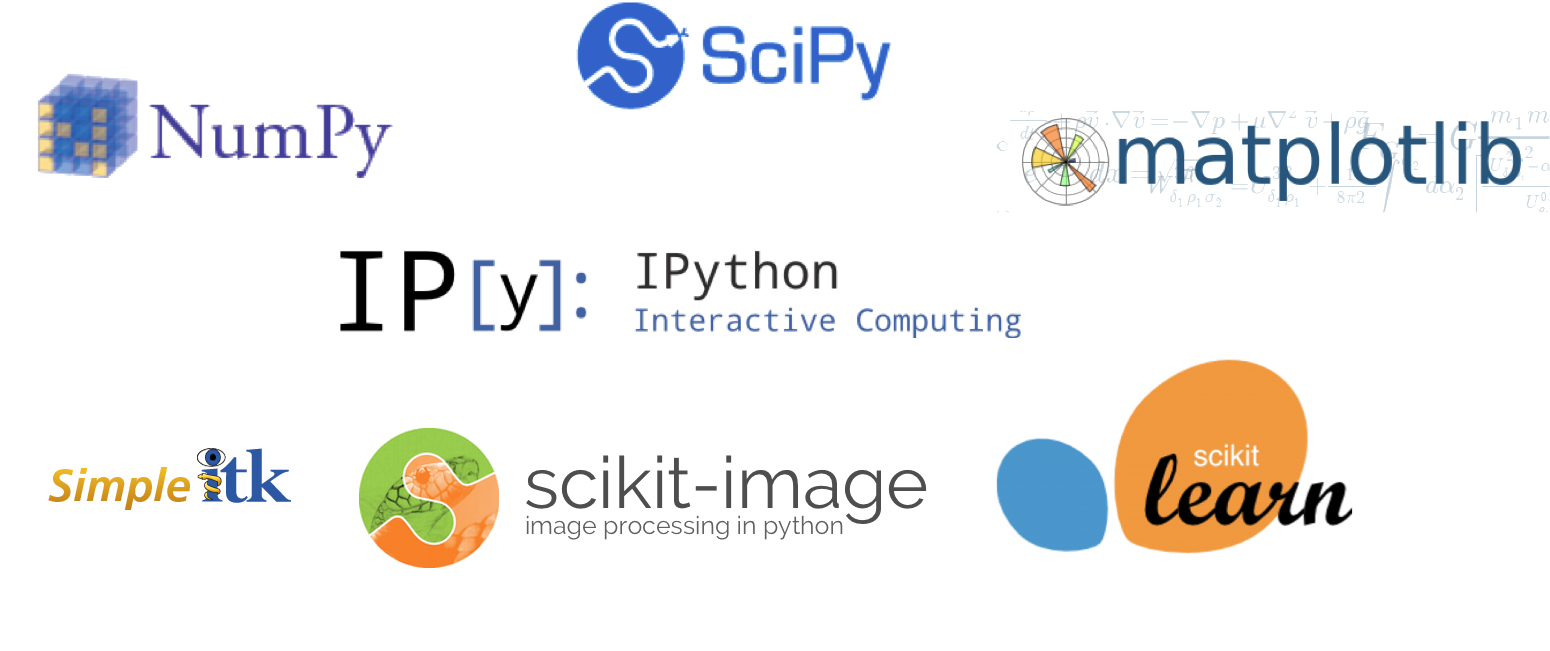
\includegraphics[width=.55\textwidth]{./images/toolbox.png}
    \end{figure}
  \end{block}
  \footcitetext{lemaitre2016imbalanced}
\end{frame}

\subsection{I2CVB}

\begin{frame}
  \frametitle{I2CVB}
  \framesubtitle{A web platform}
  \begin{block}{\small 
\includegraphics[height=.04\textheight]{./images/i2cvb/i2cvb.pdf}\ platform}
    \begin{figure}
      \centering
      
\includegraphics[width=.8\linewidth]{./images/i2cvb/website.pdf}
    \end{figure}
  \end{block}
  \begin{block}{\small Hub for our different resources}
    \begin{itemize}\scriptsize
    \item GitHub for our source codes
    \item Zenodo for our datasets
    \item HAL, arXiv, ResearchGate for our publications
    \end{itemize}
  \end{block}
\end{frame}

% \begin{frame}
%   \frametitle{I2CVB}
%   \framesubtitle{Manifesto}
%   \begin{columns}
%     \column{.5\textwidth}
%     \begin{block}{\small 
\includegraphics[height=.04\textheight]{./images/i2cvb/i2cvb.pdf}\ Vision}
%       \begin{figure}
%         \centering
%         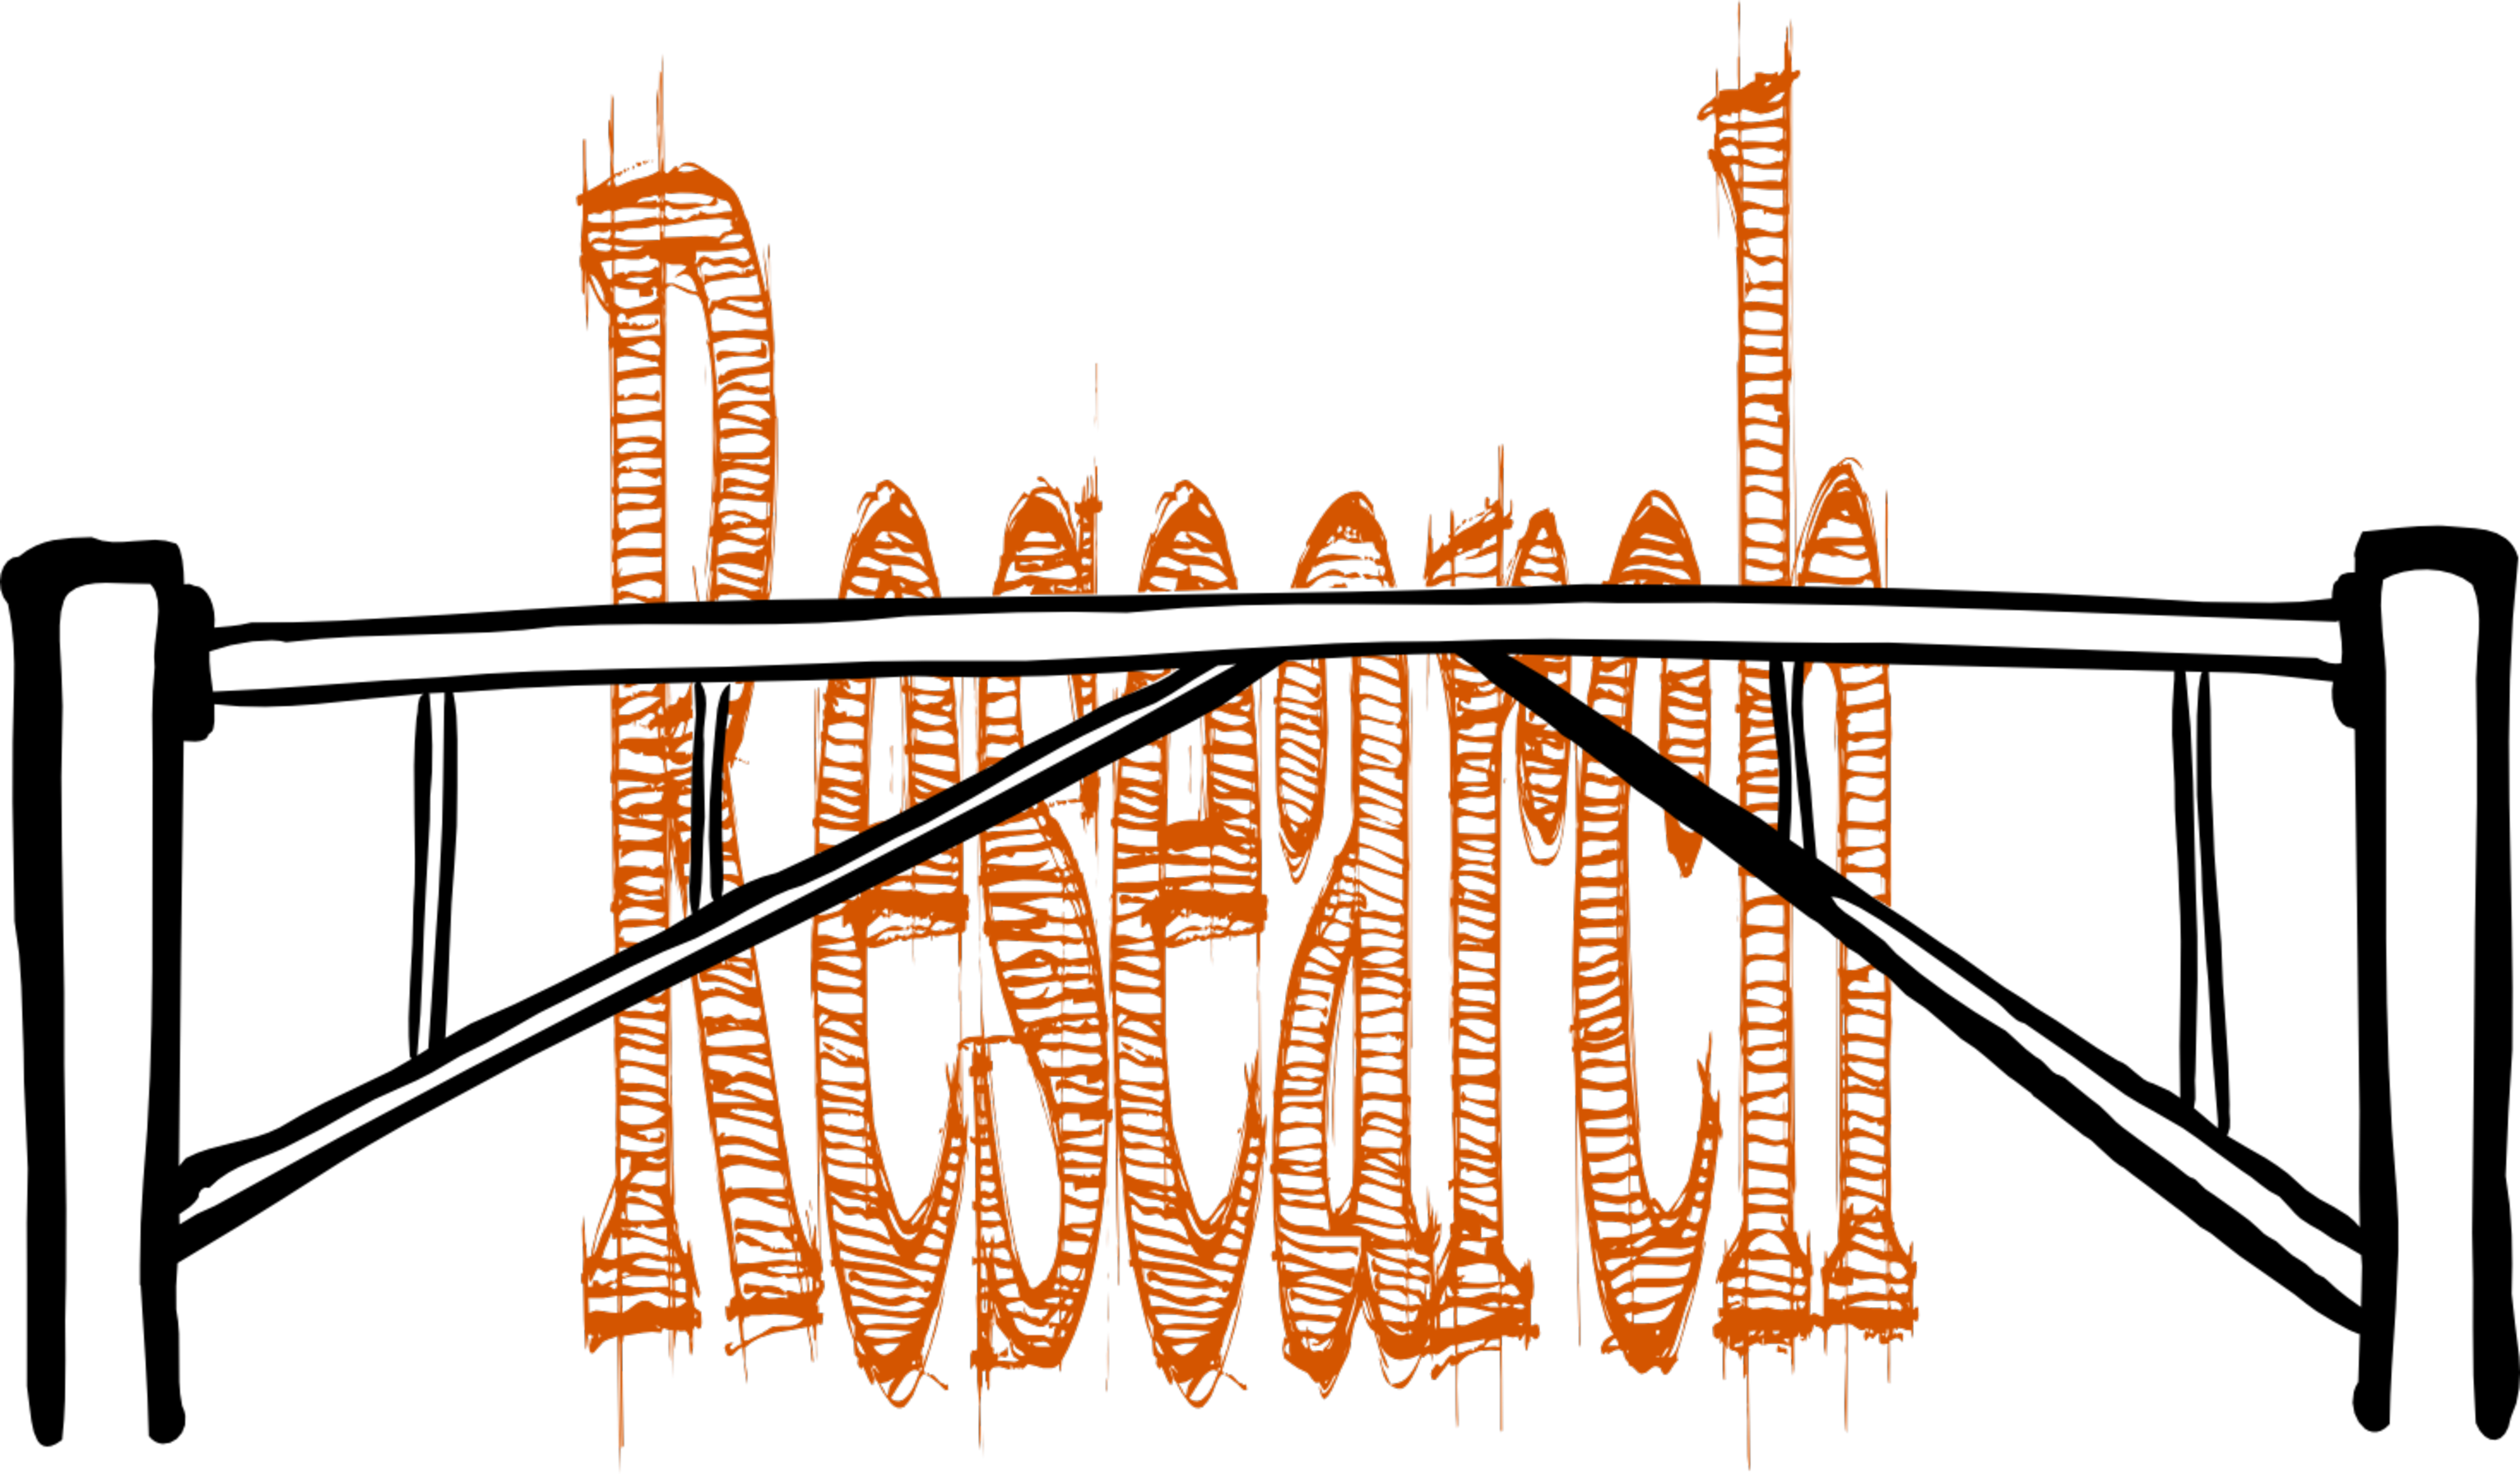
\includegraphics[height=.15\textheight]{./images/i2cvb/research.pdf}
%       \end{figure}
%       \vskip-4ex
%       \begin{itemize}\tiny
%       \item Ease the access to make research
%       \end{itemize}
%       \vskip1ex
%     \end{block}
%     \begin{block}{\small 
\includegraphics[height=.04\textheight]{./images/i2cvb/i2cvb.pdf}\ Protagonists}
%       \begin{figure}
%         \centering
%         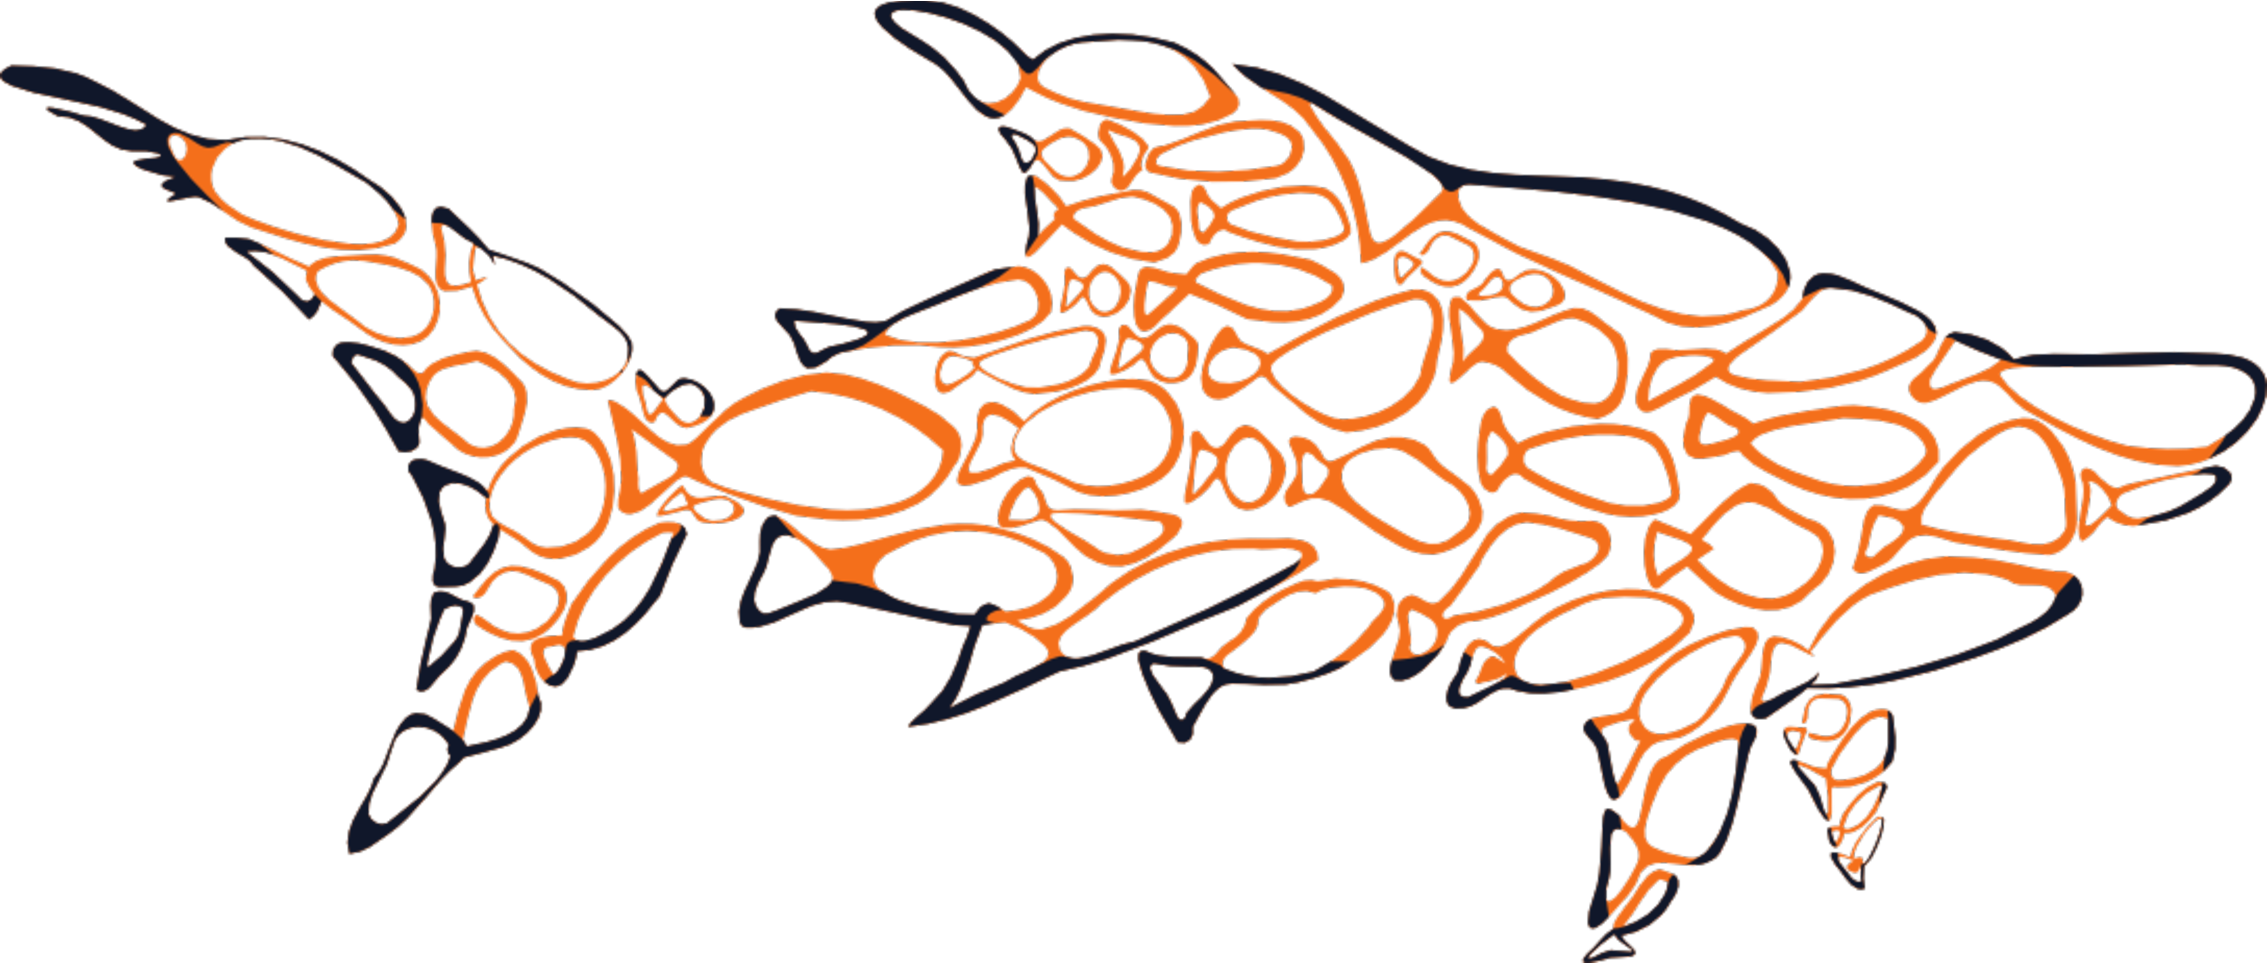
\includegraphics[height=.15\textheight]{./images/i2cvb/shark.pdf}
%       \end{figure}
%       \vskip-4ex
%       \begin{itemize}\tiny
%       \item Research groups and individuals from all walks of life to shape an open community
%       \end{itemize}
%     \end{block}
%     \column{.5\textwidth}
%     \begin{block}{\small 
\includegraphics[height=.04\textheight]{./images/i2cvb/i2cvb.pdf}\ Mission}
%       \begin{figure}
%         \centering
%         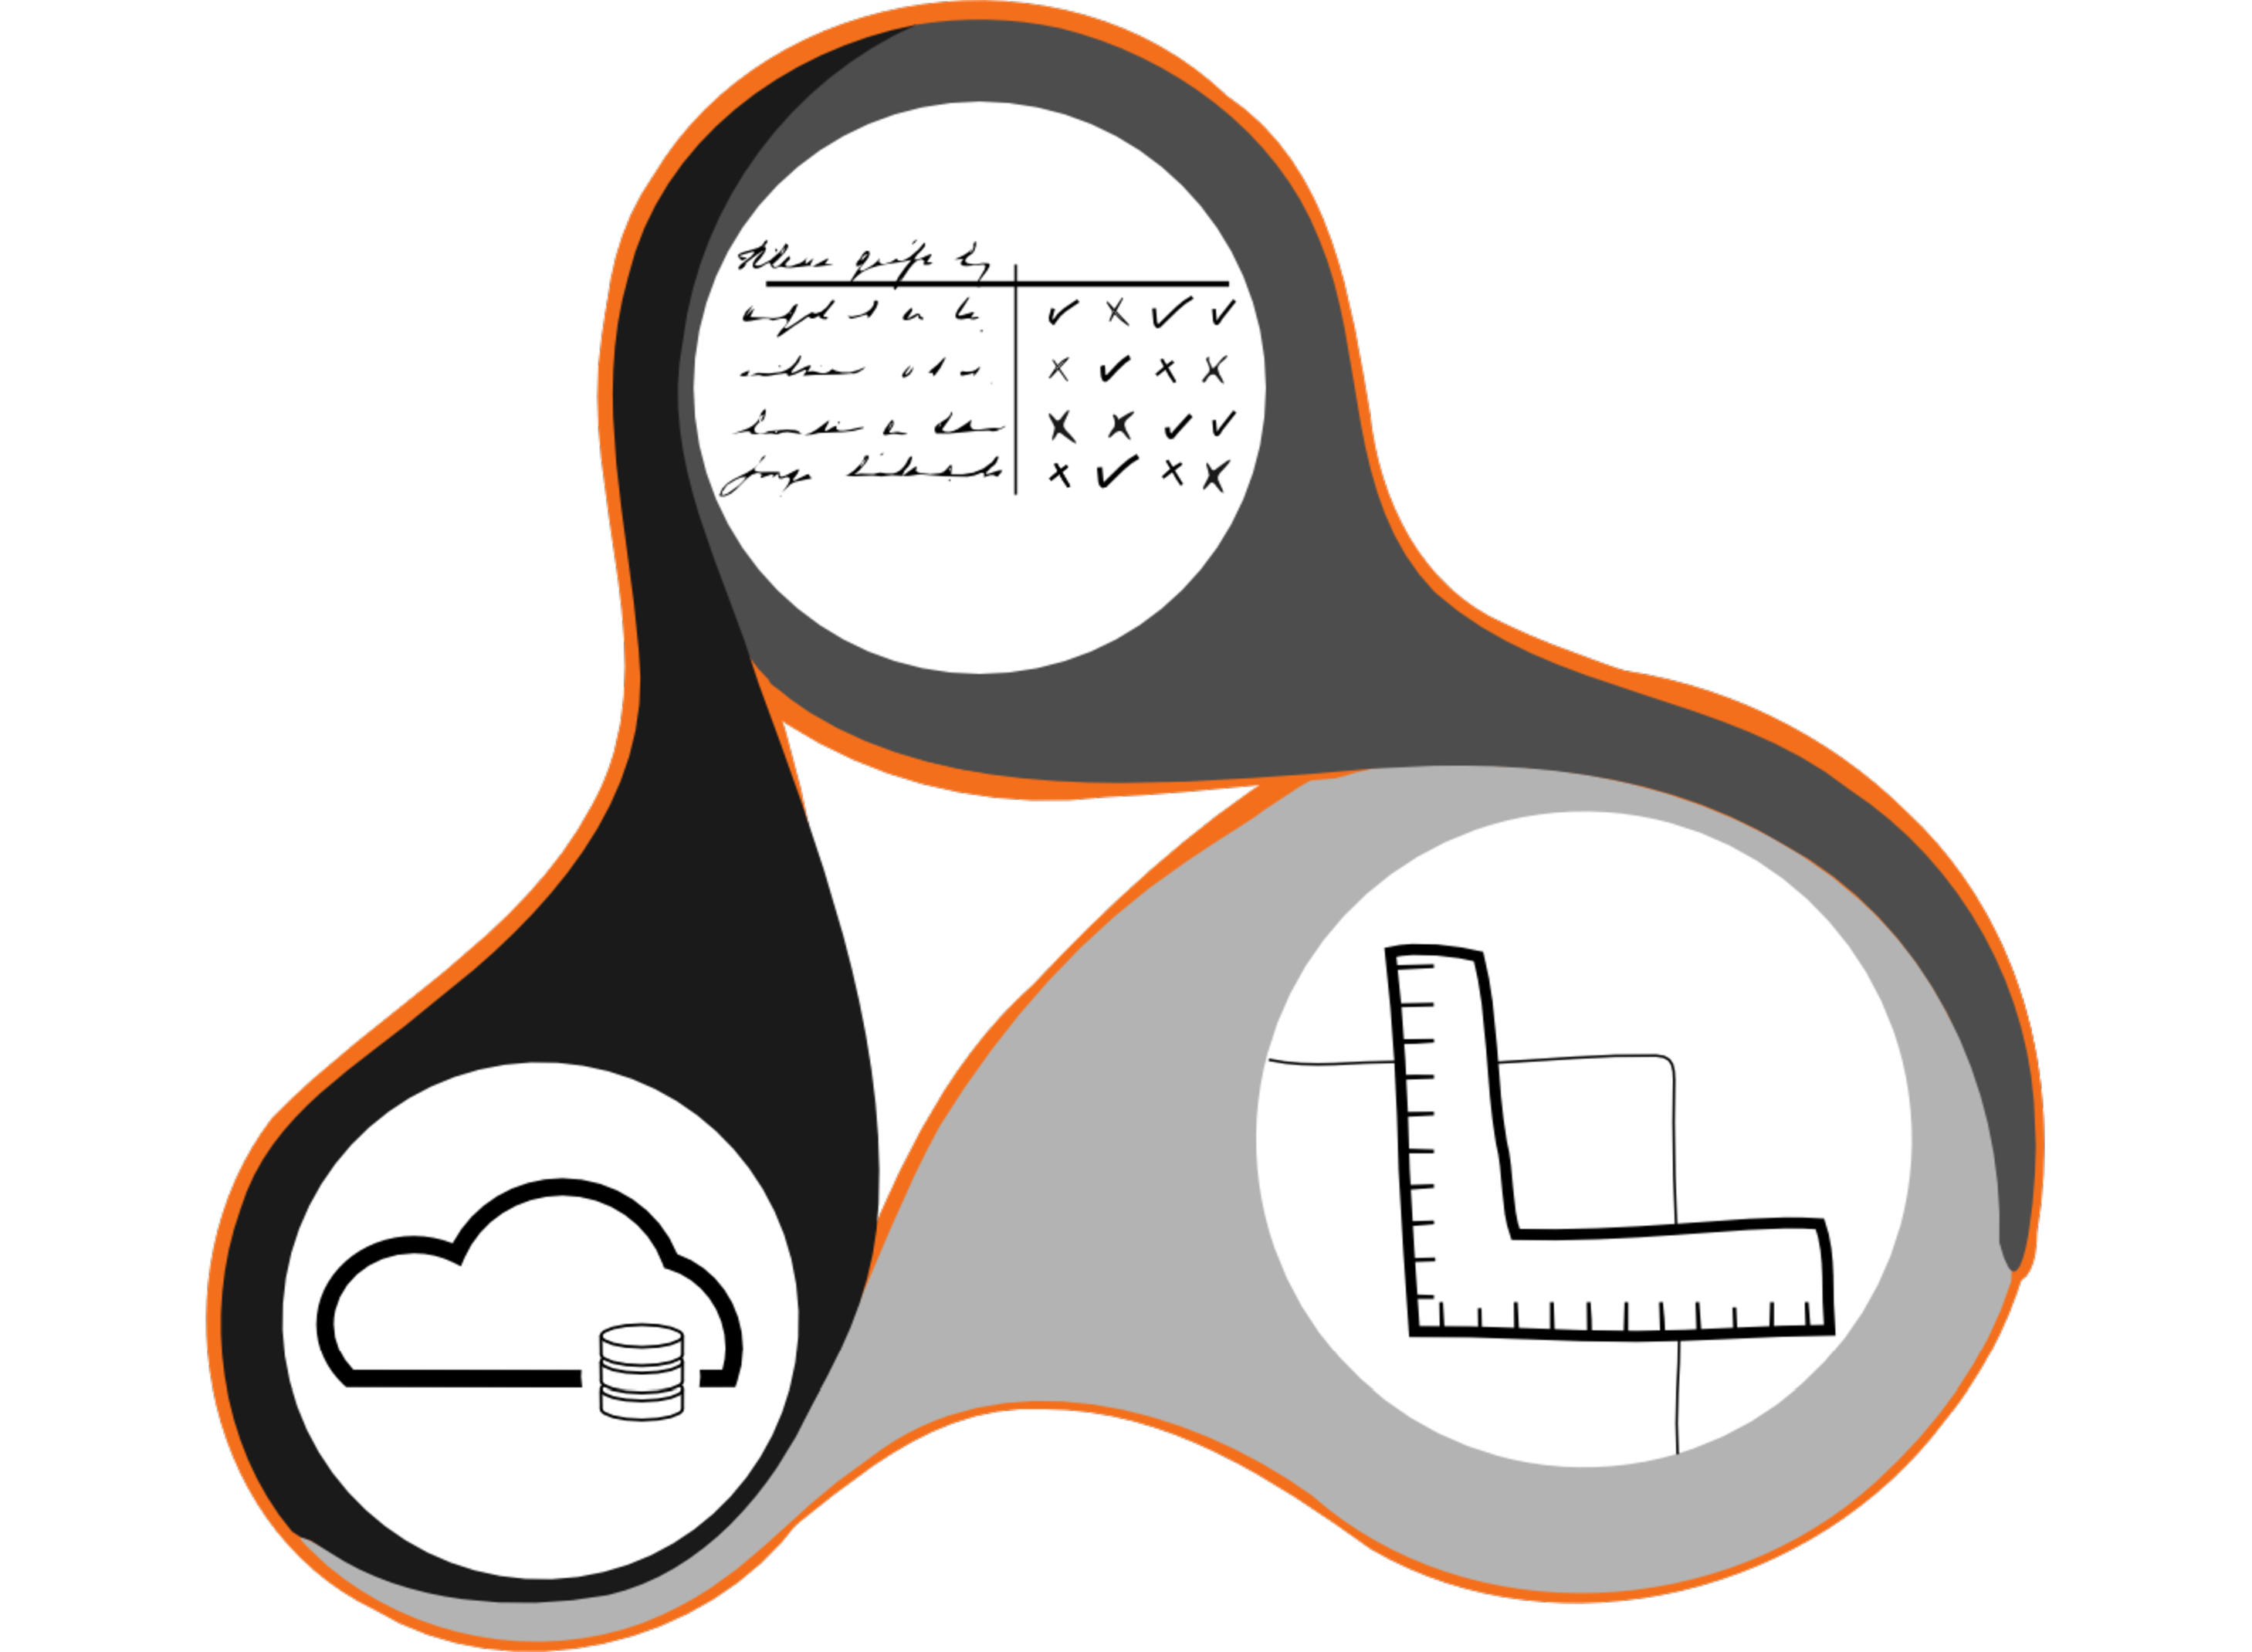
\includegraphics[height=.15\textheight]{./images/i2cvb/what.pdf}
%       \end{figure}
%       \vskip-4ex
%       \begin{itemize}\tiny
%       \item Open data; evaluation methods; comparison framework; reporting platform
%       \end{itemize}
%     \end{block}
%     \begin{block}{\small 
\includegraphics[height=.04\textheight]{./images/i2cvb/i2cvb.pdf}\ Strategy}
%       \begin{figure}
%         \centering
%         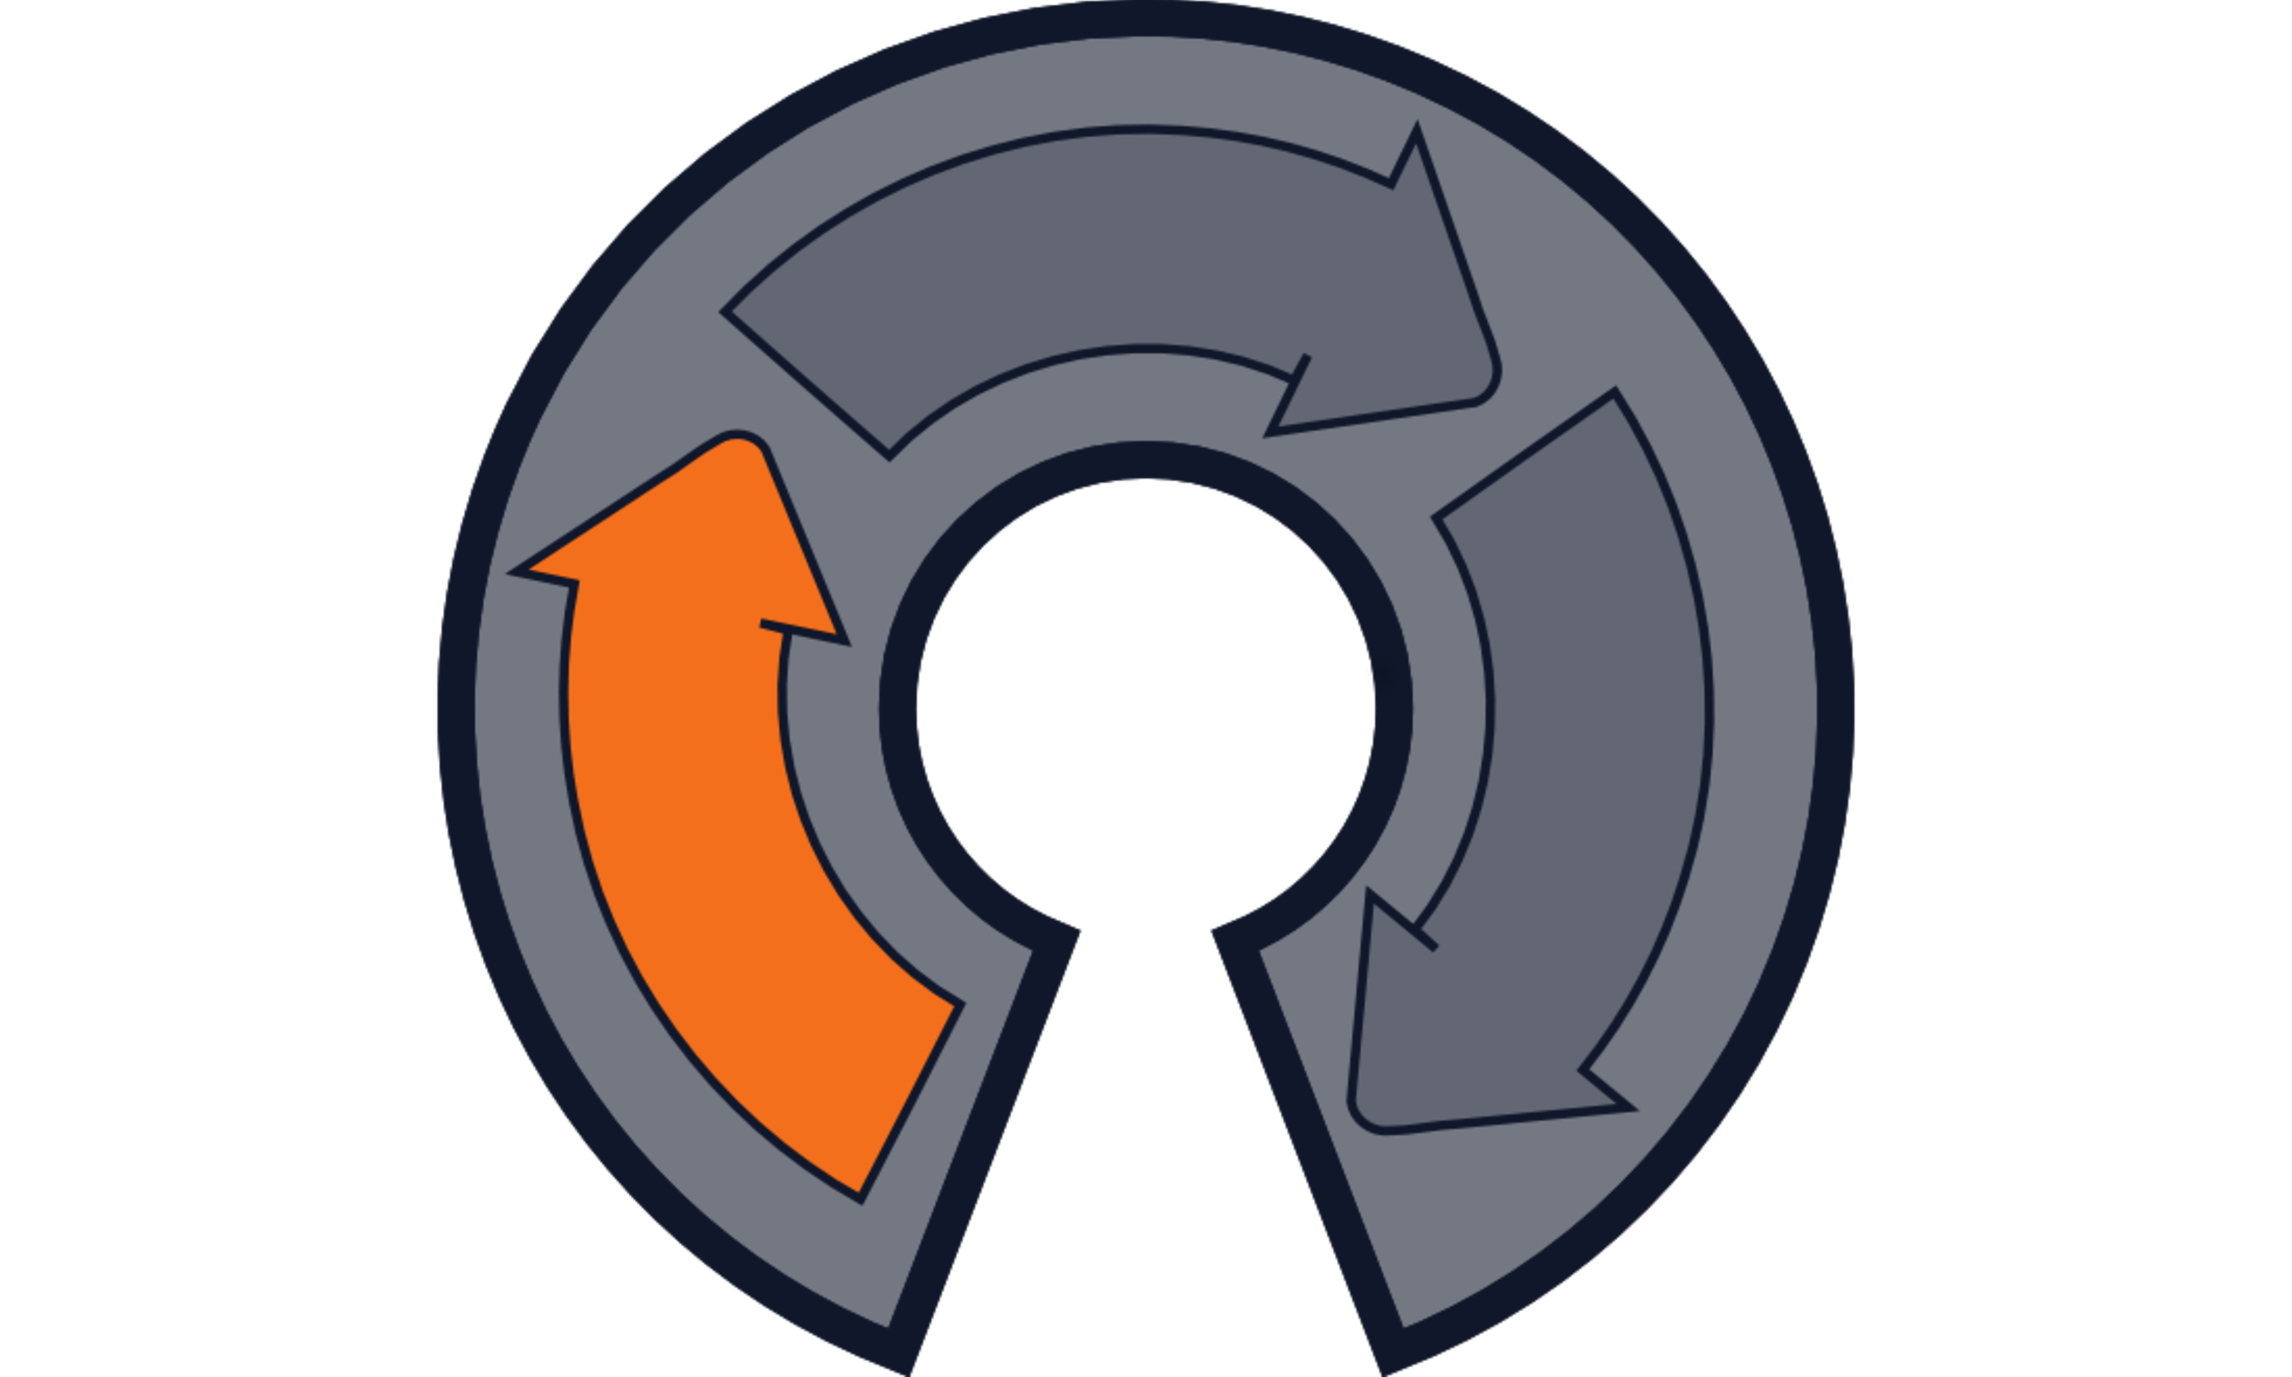
\includegraphics[height=.15\textheight]{./images/i2cvb/open.pdf}
%       \end{figure}
%       \vskip-4ex
%       \begin{itemize}\tiny
%       \item Use successful practises from Free Software and Quality Management
%       \end{itemize}
%       \vskip1ex
%     \end{block}
%   \end{columns}
% \end{frame}

\section{Toward a mp-MRI CAD for CaP}

\begin{frame}
  \begin{scriptsize}
    \tableofcontents[currentsection,currentsubsection,subsectionstyle=show/show/hide,subsubsectionstyle=hide]
  \end{scriptsize}
\end{frame}

\subsection{Image regularization}

\subsubsection{Pre-processing}

\begin{frame}
  \frametitle{Toward a mp-MRI CAD for CaP}
  \framesubtitle{Toward a mp-MRI CAD for CaP}
  \begin{block}{\small Mp-MRI CAD for CaP}
    \begin{figure}
  \centering

  % Define block styles used later

  \tikzstyle{module}=[draw, draw=azulunam!80, text width=10em, 
  text centered, minimum height=5em, minimum width = 15em, drop shadow, rounded corners,
  fill=azulunam!30]
  \tikzstyle{moduleorange}=[draw, draw=orangeubfc!80, text width=10em, 
  text centered, minimum height=5em, minimum width = 15em, drop shadow, rounded corners,
  fill=orangeubfc!30]
  
  \tikzstyle{vecArrow} = [thick, decoration={markings,mark=at position
    1 with {\arrow[semithick]{open triangle 60}}},
  double distance=1.4pt, shorten >= 5.5pt,
  preaction = {decorate},
  postaction = {draw,line width=1.4pt, white,shorten >= 4.5pt}]

  % Define distances for bordering
  \def\blockdist{1.5}
  \def\edgedist{2.5}

  \begin{tikzpicture}[node distance=3cm,thick,scale=0.38, every node/.style={scale=0.38},path image/.style={
      path picture={
        \node at (path picture bounding box.center) {
          \includegraphics[width=1cm]{#1}
        };}}]
    \tikzstyle{conefill} = [path image=,fill opacity=0.8]
    \node[module=above:pre] (pre) at (4.5,-2.6) {\Large Pre-processing};
    \node[module,below of=pre] (seg) {\Large Segmentation};
    \node[module,below of=seg] (reg) {\Large Registration};

    \path[->,dashed] (seg.west) edge [bend right=70] node {} (reg.west);
    \path[->,dashed] (reg.east) edge [bend right=70] node {} (seg.east);

    \draw[->] (pre)--(seg);
    \draw[->] (seg)--(reg);

    \begin{pgfonlayer}{background}
      \path (pre.west |- pre.north)+(-0.9,1.0+\blockdist) node (a) {};
      \path (reg.east |- reg.south)+(+0.9,-0.5) node (b) {};
      
      \path[fill=azulunam!10,rounded corners, draw=azulunam!20, dashed] (a) rectangle (b);
    \end{pgfonlayer}
    
    \path (pre.north) +(0,+\blockdist) node (bgreg) {\Large Image regularization};

    \begin{scope}[node distance=10cm]
      \node[module] (det) [below right=0cm and 2cm of pre] {\Large Features detection};
    \end{scope}
    \begin{scope}[node distance=3.5cm]
      \node[module,above of=det] (roi) {\Large ROIs\\detection/selection};
    \end{scope}
    \node[module,below of=det] (sel) {\Large Data\\balancing};
    \node[module,below of=sel] (bal) {\Large Features\\selection/extraction};
    \node[module,below of=bal] (cla) {\Large Features\\classification/fusion};

    \draw[->] (roi)--(det);
    \draw[->] (det)--(sel);
    \draw[->] (sel)--(bal);
    \draw[->] (bal)--(cla);

    \begin{pgfonlayer}{background}
      \path (roi.west |- roi.north)+(-0.25,0.8) node (c) {};
      \path (roi.east |- roi.south)+(+0.25,-0.25) node (d) {};
      
      \path[fill=azulunam!20,rounded corners, draw=azulunam!25, dashed] (c) rectangle (d);
    \end{pgfonlayer}

    \path (roi.west |- roi.north) +(.75,0.4) node (bgfea) {\Large \textbf{CADe}};

    \begin{pgfonlayer}{background}
      \path (det.west |- det.north)+(-0.25,0.8) node (c) {};
      \path (cla.east |- cla.south)+(+0.25,-0.25) node (d) {};
      
      \path[fill=azulunam!20,rounded corners, draw=azulunam!25, dashed] (c) rectangle (d);
    \end{pgfonlayer}

    \path (roi.west |- det.north) +(.75,0.4) node (bgfea) {\Large \textbf{CADx}};     

    % \begin{scope}
    %   \transparent{0.6}\filldraw[fill=red!20!white,rounded corners,draw=red!25,dashed] (11.5,-8.7) rectangle (19,-9.8);
    % \end{scope}

    % Define the place where the arrow should start anf finish
    \path (seg.east |- seg.north)+(+1.15,0) node (e) {};
    \path (sel.west |- seg.north)+(-1.0,0) node (f) {};

    \draw[double distance =3pt,preaction={-triangle 90,thin,draw,shorten >=-1mm}] (e) -- (f) node[midway,above,above=.3em] {\large Regularized data};

    \begin{scope}[yshift=-33,xshift=-86]
      \transparent{0.6}\draw[path image=images/tikzimage/t2.eps] (0,0) rectangle (1.0,1.0);
    \end{scope}

    \begin{scope}[yshift=-36,xshift=-83]
      \transparent{0.6}\draw[path image=images/tikzimage/t2.eps] (0,0) rectangle (1.0,1.0);
    \end{scope}

    \begin{scope}[yshift=-39,xshift=-80]
      \transparent{0.8}\draw[path image=images/tikzimage/t2.eps] (0,0) rectangle (1.0,1.0);
      \path (0,0)+(-1.35,0.3) node {\Large T$_2$W-MRI};
    \end{scope}

    \begin{scope}[yshift=-100,xshift=-86]
      \transparent{0.6}\draw[path image=images/tikzimage/dce.eps] (0,0) rectangle (1.0,1.0);
    \end{scope}

    \begin{scope}[yshift=-103,xshift=-83]
      \transparent{0.6}\draw[path image=images/tikzimage/dce.eps] (0,0) rectangle (1.0,1.0);
    \end{scope}

    \begin{scope}[yshift=-106,xshift=-80]
      \transparent{0.8}\draw[path image=images/tikzimage/dce.eps] (0,0) rectangle (1.0,1.0);
      \path (0,0)+(-1.65,0.3) node {\Large DCE-MRI};
    \end{scope}

    \begin{scope}[yshift=-167,xshift=-86]
      \transparent{0.6}\draw[path image=images/tikzimage/dwi1.eps] (0,0) rectangle (1.0,1.0);
    \end{scope}

    \begin{scope}[yshift=-170,xshift=-83]
      \transparent{0.6}\draw[path image=images/tikzimage/dwi1.eps] (0,0) rectangle (1.0,1.0);
    \end{scope}

    \begin{scope}[yshift=-173,xshift=-80]
      \transparent{0.8}\draw[path image=images/tikzimage/dwi1.eps] (0,0) rectangle (1.0,1.0);
      \path (0,0)+(-1.65,0.3) node {\Large ADC};
    \end{scope}

    \begin{scope}[yshift=-234,xshift=-86]
      \transparent{0.6}\draw[path image=images/tikzimage/mrsi.eps] (0,0) rectangle (1.0,1.0);
    \end{scope}

    \begin{scope}[yshift=-237,xshift=-83]
      \transparent{0.6}\draw[path image=images/tikzimage/mrsi.eps] (0,0) rectangle (1.0,1.0);
    \end{scope}

    \begin{scope}[yshift=-240,xshift=-80]
      \transparent{0.8}\draw[path image=images/tikzimage/mrsi.eps] (0,0) rectangle (1.0,1.0);
      \path (0,0)+(-1.5,0.3) node {\Large MRSI};
    \end{scope}

    \path (pre.west |- roi.north)+(-2.5,-1.+\blockdist) node (g) {};
    \path (reg.west |- reg.south)+(-2.5,.5) node (h) {};

    \draw[decorate,decoration={brace,raise=2pt,amplitude=5pt}, thick]
    (g)--(h) ;
    
    \path (seg.west |- seg.north)+(-2.5,0) node (i) {};
    \path (seg.west |- seg.north)+(-0.9,0) node (j) {};
    
    % \draw[double distance =3pt,preaction={-triangle 90,thin,draw,shorten >=-1mm}] (i) -- (j);   

    \path (sel.east |- seg.north)+(2,0) node (k) {};
    \path (sel.east |- seg.north)+(0.5,0) node (l) {};
    
  \end{tikzpicture}
\end{figure}

%%% Local Variables: 
%%% mode: latex
%%% TeX-master: "../../presentation"
%%% End: 

  \end{block}
\end{frame}

\begin{frame}
  \frametitle{Toward a mp-MRI CAD for CaP}
  \framesubtitle{Image regularization}
  \begin{block}{\small Pre-processing}
    \begin{figure}
  \centering

  % Define block styles used later

  \tikzstyle{module}=[draw, draw=azulunam!80, text width=10em, 
  text centered, minimum height=5em, minimum width = 15em, drop shadow, rounded corners,
  fill=azulunam!30]
  \tikzstyle{moduleorange}=[draw, draw=orangeubfc!80, text width=10em, 
  text centered, minimum height=5em, minimum width = 15em, drop shadow, rounded corners,
  fill=orangeubfc!30]
  
  \tikzstyle{vecArrow} = [thick, decoration={markings,mark=at position
    1 with {\arrow[semithick]{open triangle 60}}},
  double distance=1.4pt, shorten >= 5.5pt,
  preaction = {decorate},
  postaction = {draw,line width=1.4pt, white,shorten >= 4.5pt}]

  % Define distances for bordering
  \def\blockdist{1.5}
  \def\edgedist{2.5}

  \begin{tikzpicture}[node distance=3cm,thick,scale=0.3, every node/.style={scale=0.3},path image/.style={
      path picture={
        \node at (path picture bounding box.center) {
          \includegraphics[width=1cm]{#1}
        };}}]
    \tikzstyle{conefill} = [path image=,fill opacity=0.8]
    \node[moduleorange=above:pre] (pre) at (4.5,-2.6) {\Large Pre-processing};
    \node[module,below of=pre] (seg) {\Large Segmentation};
    \node[module,below of=seg] (reg) {\Large Registration};

    \path[->,dashed] (seg.west) edge [bend right=70] node {} (reg.west);
    \path[->,dashed] (reg.east) edge [bend right=70] node {} (seg.east);

    \draw[->] (pre)--(seg);
    \draw[->] (seg)--(reg);

    \begin{pgfonlayer}{background}
      \path (pre.west |- pre.north)+(-0.9,1.0+\blockdist) node (a) {};
      \path (reg.east |- reg.south)+(+0.9,-0.5) node (b) {};
      
      \path[fill=azulunam!10,rounded corners, draw=azulunam!20, dashed] (a) rectangle (b);
    \end{pgfonlayer}
    
    \path (pre.north) +(0,+\blockdist) node (bgreg) {\Large Image regularization};

    \begin{scope}[node distance=10cm]
      \node[module] (det) [below right=0cm and 2cm of pre] {\Large Features detection};
    \end{scope}
    \begin{scope}[node distance=3.5cm]
      \node[module,above of=det] (roi) {\Large ROIs\\detection/selection};
    \end{scope}
    \node[module,below of=det] (sel) {\Large Data\\balancing};
    \node[module,below of=sel] (bal) {\Large Features\\selection/extraction};
    \node[module,below of=bal] (cla) {\Large Features\\classification/fusion};

    \draw[->] (roi)--(det);
    \draw[->] (det)--(sel);
    \draw[->] (sel)--(bal);
    \draw[->] (bal)--(cla);

    \begin{pgfonlayer}{background}
      \path (roi.west |- roi.north)+(-0.25,0.8) node (c) {};
      \path (roi.east |- roi.south)+(+0.25,-0.25) node (d) {};
      
      \path[fill=azulunam!20,rounded corners, draw=azulunam!25, dashed] (c) rectangle (d);
    \end{pgfonlayer}

    \path (roi.west |- roi.north) +(.75,0.4) node (bgfea) {\Large \textbf{CADe}};

    \begin{pgfonlayer}{background}
      \path (det.west |- det.north)+(-0.25,0.8) node (c) {};
      \path (cla.east |- cla.south)+(+0.25,-0.25) node (d) {};
      
      \path[fill=azulunam!20,rounded corners, draw=azulunam!25, dashed] (c) rectangle (d);
    \end{pgfonlayer}

    \path (roi.west |- det.north) +(.75,0.4) node (bgfea) {\Large \textbf{CADx}};     

    % \begin{scope}
    %   \transparent{0.6}\filldraw[fill=red!20!white,rounded corners,draw=red!25,dashed] (11.5,-8.7) rectangle (19,-9.8);
    % \end{scope}

    % Define the place where the arrow should start anf finish
    \path (seg.east |- seg.north)+(+1.15,0) node (e) {};
    \path (sel.west |- seg.north)+(-1.0,0) node (f) {};

    \draw[double distance =3pt,preaction={-triangle 90,thin,draw,shorten >=-1mm}] (e) -- (f) node[midway,above,above=.3em] {\large Regularized data};

    \begin{scope}[yshift=-33,xshift=-86]
      \transparent{0.6}\draw[path image=images/tikzimage/t2.eps] (0,0) rectangle (1.0,1.0);
    \end{scope}

    \begin{scope}[yshift=-36,xshift=-83]
      \transparent{0.6}\draw[path image=images/tikzimage/t2.eps] (0,0) rectangle (1.0,1.0);
    \end{scope}

    \begin{scope}[yshift=-39,xshift=-80]
      \transparent{0.8}\draw[path image=images/tikzimage/t2.eps] (0,0) rectangle (1.0,1.0);
      \path (0,0)+(-1.35,0.3) node {\Large T$_2$W-MRI};
    \end{scope}

    \begin{scope}[yshift=-100,xshift=-86]
      \transparent{0.6}\draw[path image=images/tikzimage/dce.eps] (0,0) rectangle (1.0,1.0);
    \end{scope}

    \begin{scope}[yshift=-103,xshift=-83]
      \transparent{0.6}\draw[path image=images/tikzimage/dce.eps] (0,0) rectangle (1.0,1.0);
    \end{scope}

    \begin{scope}[yshift=-106,xshift=-80]
      \transparent{0.8}\draw[path image=images/tikzimage/dce.eps] (0,0) rectangle (1.0,1.0);
      \path (0,0)+(-1.65,0.3) node {\Large DCE-MRI};
    \end{scope}

    \begin{scope}[yshift=-167,xshift=-86]
      \transparent{0.6}\draw[path image=images/tikzimage/dwi1.eps] (0,0) rectangle (1.0,1.0);
    \end{scope}

    \begin{scope}[yshift=-170,xshift=-83]
      \transparent{0.6}\draw[path image=images/tikzimage/dwi1.eps] (0,0) rectangle (1.0,1.0);
    \end{scope}

    \begin{scope}[yshift=-173,xshift=-80]
      \transparent{0.8}\draw[path image=images/tikzimage/dwi1.eps] (0,0) rectangle (1.0,1.0);
      \path (0,0)+(-1.65,0.3) node {\Large ADC};
    \end{scope}

    \begin{scope}[yshift=-234,xshift=-86]
      \transparent{0.6}\draw[path image=images/tikzimage/mrsi.eps] (0,0) rectangle (1.0,1.0);
    \end{scope}

    \begin{scope}[yshift=-237,xshift=-83]
      \transparent{0.6}\draw[path image=images/tikzimage/mrsi.eps] (0,0) rectangle (1.0,1.0);
    \end{scope}

    \begin{scope}[yshift=-240,xshift=-80]
      \transparent{0.8}\draw[path image=images/tikzimage/mrsi.eps] (0,0) rectangle (1.0,1.0);
      \path (0,0)+(-1.5,0.3) node {\Large MRSI};
    \end{scope}

    \path (pre.west |- roi.north)+(-2.5,-1.+\blockdist) node (g) {};
    \path (reg.west |- reg.south)+(-2.5,.5) node (h) {};

    \draw[decorate,decoration={brace,raise=2pt,amplitude=5pt}, thick]
    (g)--(h) ;
    
    \path (seg.west |- seg.north)+(-2.5,0) node (i) {};
    \path (seg.west |- seg.north)+(-0.9,0) node (j) {};
    
    % \draw[double distance =3pt,preaction={-triangle 90,thin,draw,shorten >=-1mm}] (i) -- (j);   

    \path (sel.east |- seg.north)+(2,0) node (k) {};
    \path (sel.east |- seg.north)+(0.5,0) node (l) {};
    
  \end{tikzpicture}
\end{figure}

%%% Local Variables: 
%%% mode: latex
%%% TeX-master: "../../presentation"
%%% End: 

  \end{block}
\end{frame}

\begin{frame}
  \frametitle{Toward a mp-MRI CAD for CaP}
  \framesubtitle{Pre-processing}
  \begin{columns}
    \begin{column}{.5\textwidth}
      \begin{block}{\small T$_2$W-MRI normalization}
        \begin{itemize}\scriptsize
        \item Rician normalization\footnotemark
        \end{itemize}
      \end{block}
      \begin{block}{\small DCE-MRI normalization}
        \begin{itemize}\scriptsize
        \item Graph and deviation based normalization\footnotemark
        \end{itemize}
      \end{block}
    \end{column}
    \begin{column}{.5\textwidth}
      \begin{block}{\small ADC normalization}
        \begin{itemize}\scriptsize
        \item Piecewise-linear normalization
        \end{itemize}
      \end{block}
      \begin{block}{\small MRSI normalization}
        \begin{itemize}\scriptsize
        \item Phase correction\footnotemark
        \item Frequency alignment
        \item Baseline correction\footnotemark
        \end{itemize}
      \end{block}
    \end{column}
  \end{columns}
  \addtocounter{footnote}{-3}
  \stepcounter{footnote} \footcitetext{lemaitre2017automatic}
  \stepcounter{footnote} \footcitetext{lemaitre2016normalization}
  \stepcounter{footnote} \footcitetext{Chen2002}
  \stepcounter{footnote} \footcitetext{xi2008baseline}
\end{frame}

\begin{frame}
  \frametitle{Toward a mp-MRI CAD for CaP}
  \framesubtitle{DCE-MRI normalization}
  \begin{block}{\small Inter-patients variations}
    \begin{figure}%
      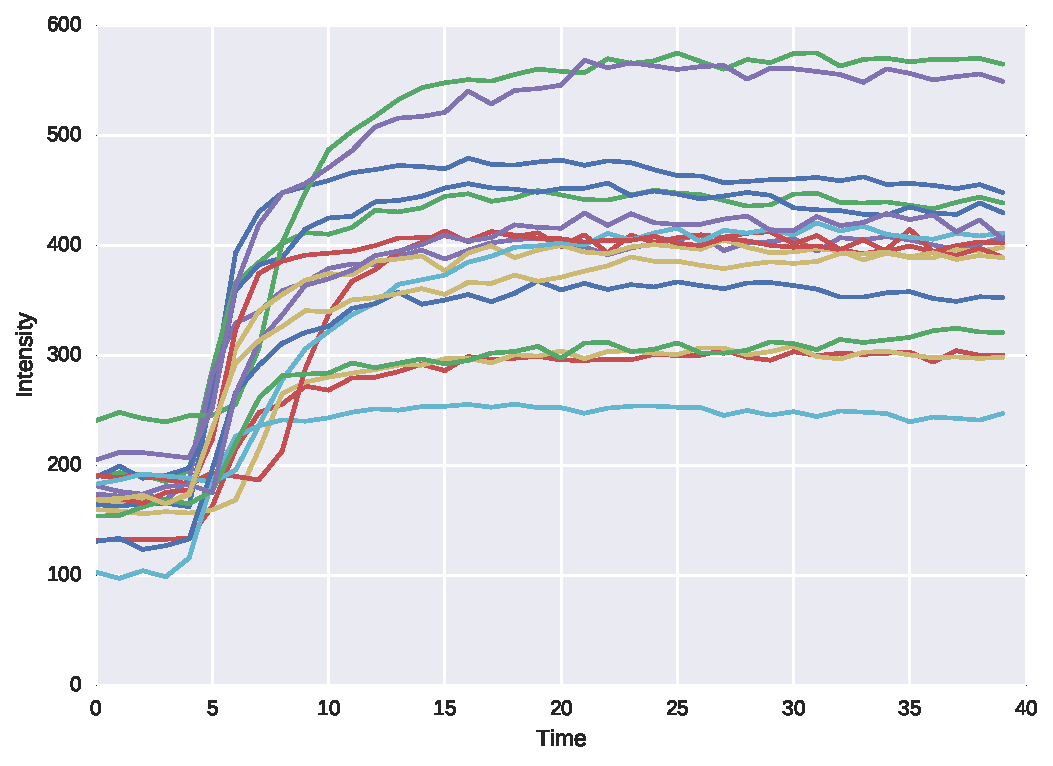
\includegraphics[width=.52\textwidth]{./images/dce_variations.pdf}
    \end{figure}
  \end{block}
  \begin{greenblock}{\small Contribution\footnotemark}
    \begin{itemize}\scriptsize
    \item Propose a method to normalize DCE-MRI data
    \end{itemize}
  \end{greenblock}
  \footcitetext{lemaitre2017automatic}
\end{frame}

\begin{frame}
  \frametitle{Toward a mp-MRI CAD for CaP}
  \framesubtitle{DCE-MRI normalization}
  \begin{block}{\small Heatmap representation}
    \begin{figure}%
      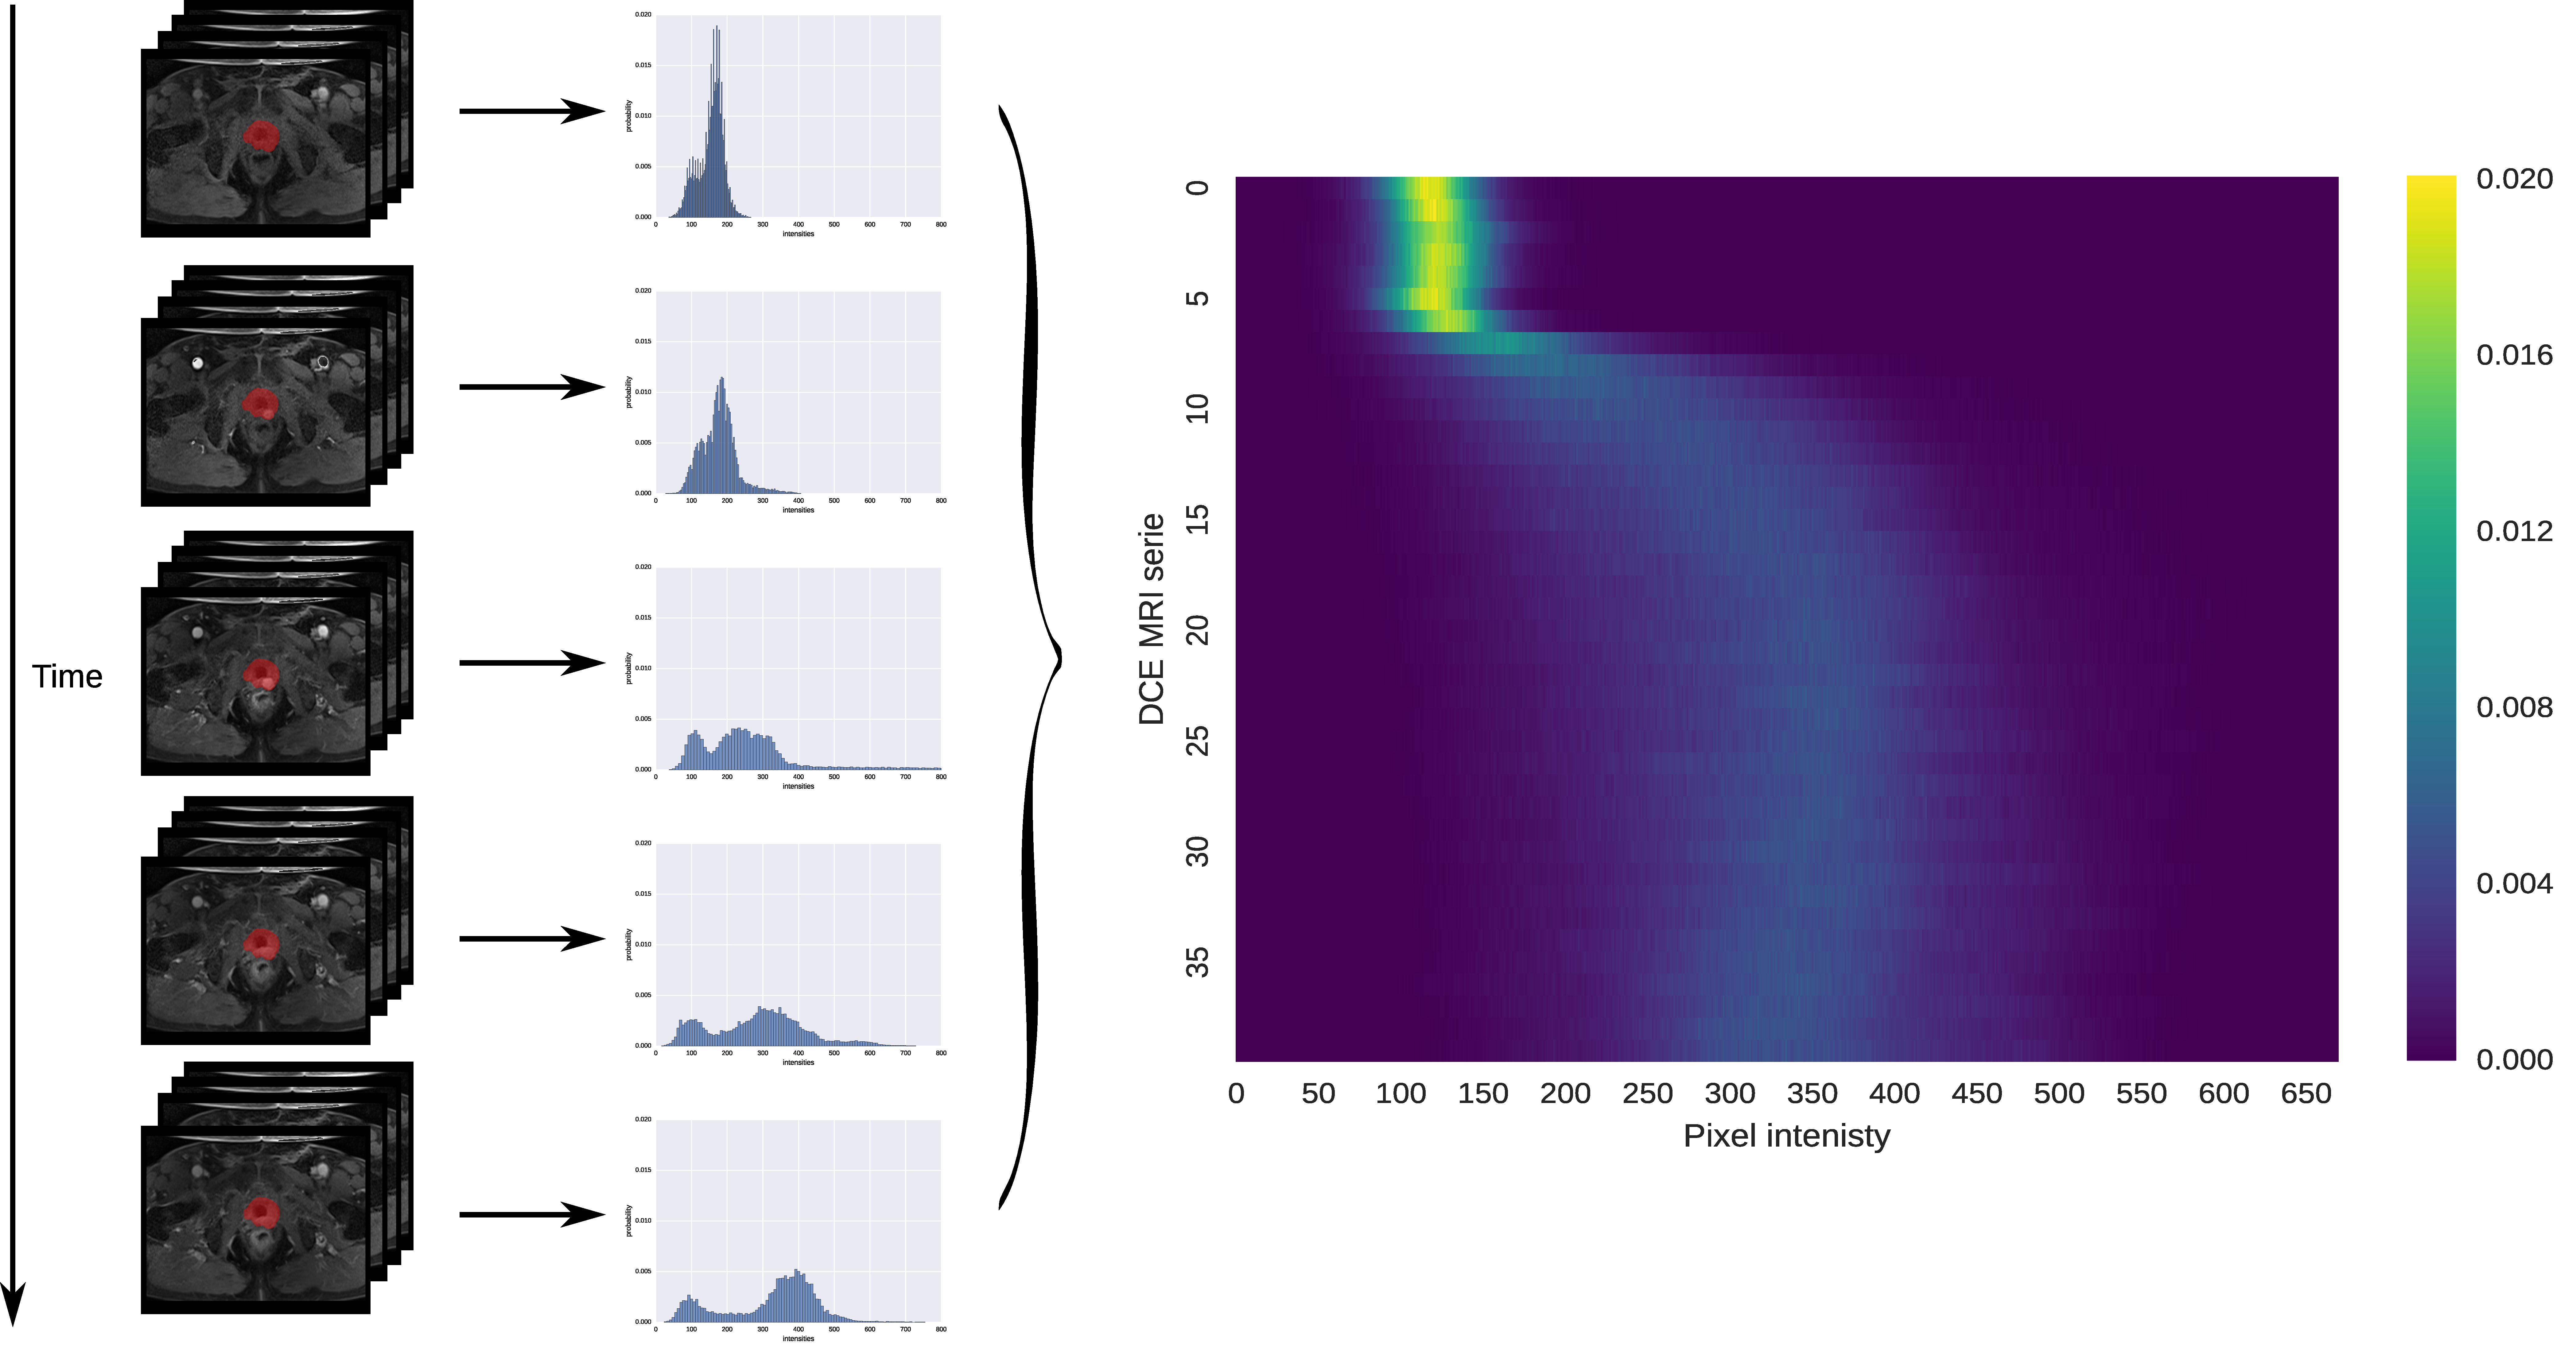
\includegraphics[width=.7\textwidth]{./images/DCE-normalization/heatmaprep.pdf}
    \end{figure}
  \end{block}
  \footcitetext{lemaitre2017automatic}
\end{frame}

\setcounter{subfigure}{0}% Reset subfigure counter

\begin{frame}
  \frametitle{Toward a mp-MRI CAD for CaP}
  \framesubtitle{DCE-MRI normalization}
  \begin{block}{\small Inter-patients variations}
    \begin{figure}%
      \centering
      \hspace*{\fill}%
      \subfigure[][\tiny Patient \#1]{%
        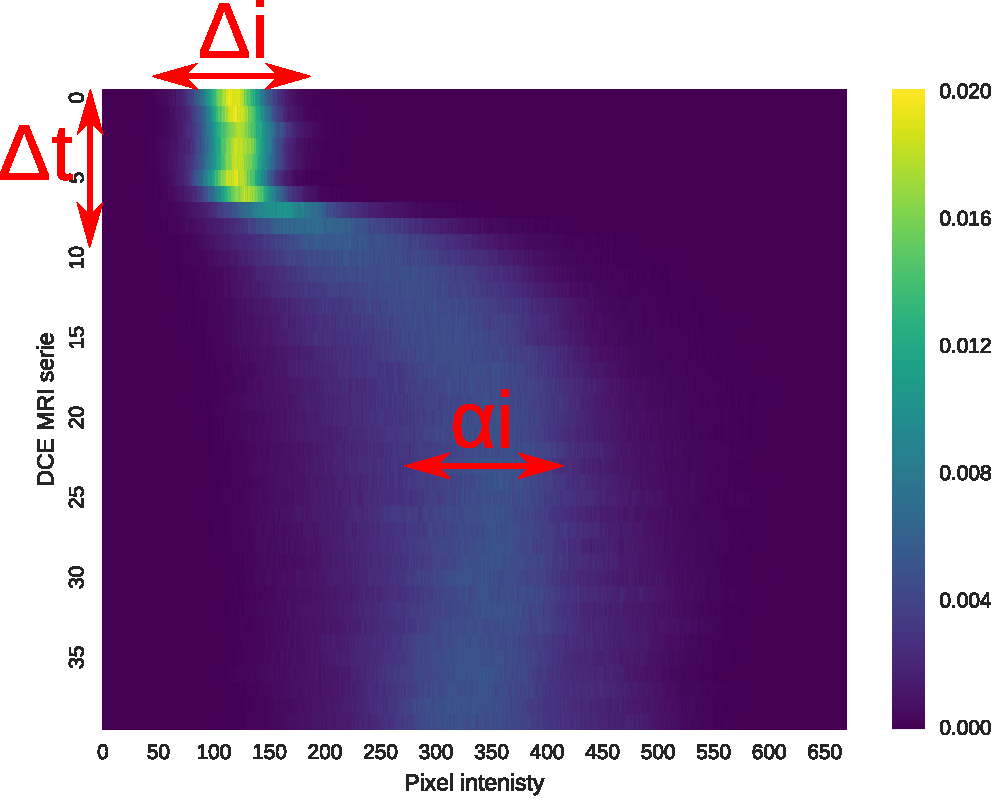
\includegraphics[width=.45\textwidth]{./images/DCE-normalization/pat1_annotated.pdf}}%
      \hfill%
      \subfigure[][\tiny Patient \#2]{%
        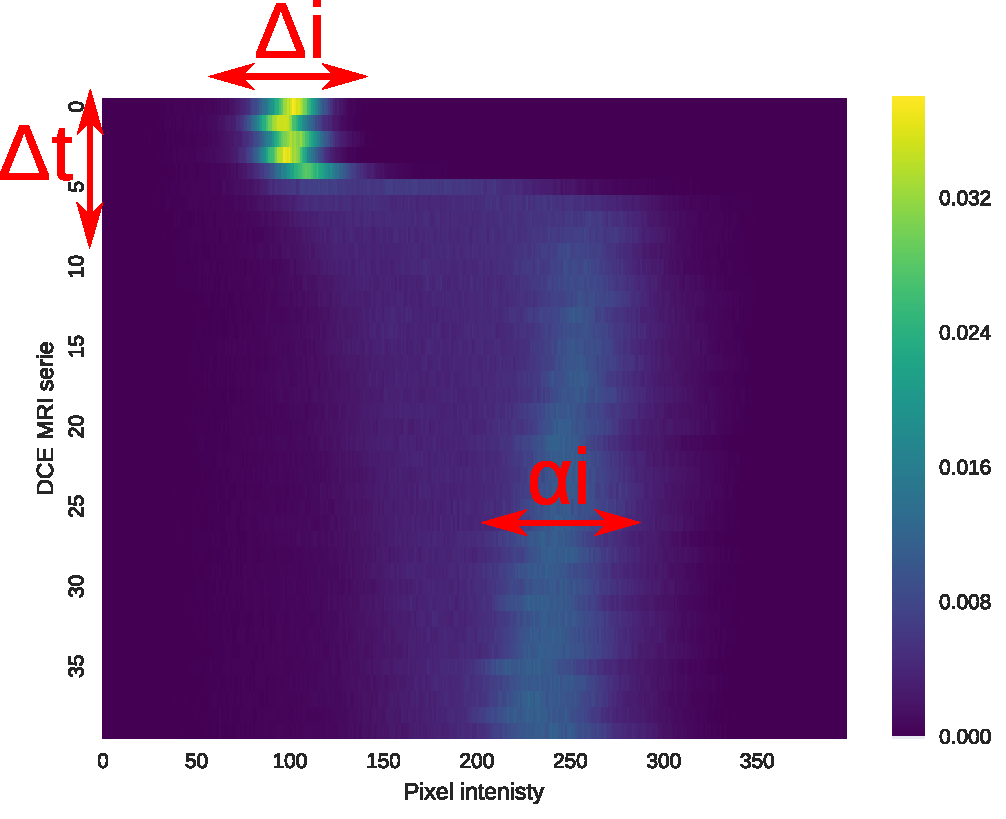
\includegraphics[width=.45\textwidth]{./images/DCE-normalization/pat2_annotated.pdf}}%
      \hspace*{\fill}%
      \caption{\tiny Variations driven by $\Delta_i$, $\Delta_t$, and $\alpha_i$}
    \end{figure}
  \end{block}
\end{frame}

\begin{frame}
  \frametitle{Toward a mp-MRI CAD for CaP}
  \framesubtitle{DCE-MRI normalization}
  \begin{block}{\small Correction of $\Delta_i$}\scriptsize
    \begin{itemize} \scriptsize
      \item Estimate with smooth transitions
      \item Estimate the closest of the PDF peak
      \item[$\rightarrow$] Find the shortest path in a directed weighted graph, with the edge weight $w_{ij}$:
        \begin{equation}\tiny
          w_{ij} = \begin{cases}
            \alpha \exp(1 - \frac{H(i)}{\max(H)})       & \text{if } x_j = x_i + 1 \text{ and } y_j = y_i, \\
            (1 - \alpha) \exp(1 - \frac{H(i)}{\max(H)}) & \text{if } x_j = x_i \text{ and } y_j = y_i + 1, \\
            0                                           & \text{otherwise},
          \end{cases}
    \end{equation}
    \end{itemize}
    \vspace*{-.5cm}
    \begin{figure}%
      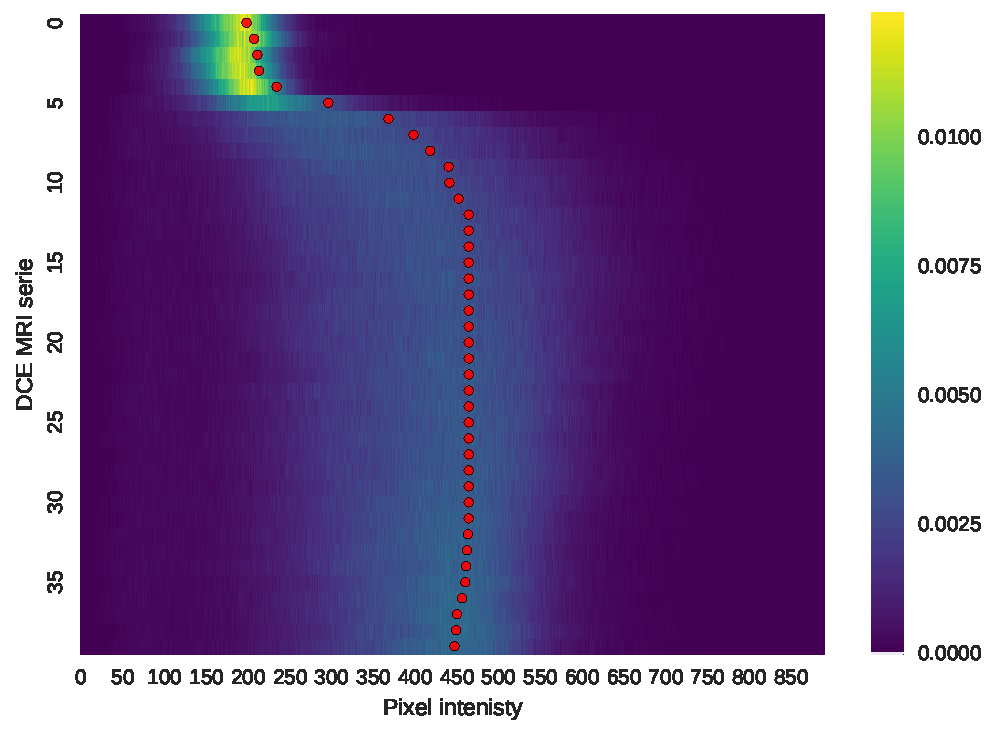
\includegraphics[width=.45\textwidth]{./images/DCE-normalization/estimator.pdf}
    \end{figure}
  \end{block}
\end{frame}

\setcounter{subfigure}{0}% Reset subfigure counter

\begin{frame}
  \frametitle{Toward a mp-MRI CAD for CaP}
  \framesubtitle{DCE-MRI normalization}
  \begin{block}{\small Correction of $\Delta_t$ and $\alpha_i$}\scriptsize
    Register all RMSD to a mean model such that:
    \vspace*{-.2cm}
    \begin{equation}\tiny
      \argmin_{\alpha, \tau} = \sum_{t=1}^{N} \left[ T\left(\alpha, \tau, f(t)\right) - \mu(t) \right]^{2} ,
      \label{eq:cost}
    \end{equation}
    \vspace*{-.3cm}
    \begin{equation}\tiny
      f(t) = \sqrt{ \left( \frac{\sum_{n=1}^{N} x(t)_{n}^2}{N}  \right) },
      \label{eq:rmsd}
    \end{equation}\tiny
    \begin{equation}
      T(\alpha, \tau, f(t)) = \alpha f(t - \tau) .
      \label{eq:model}
    \end{equation}
    \vspace*{-.7cm}
    \begin{figure}%
      \centering
      \hspace*{\fill}%
      \subfigure[][\tiny RMSD before correction]{%
        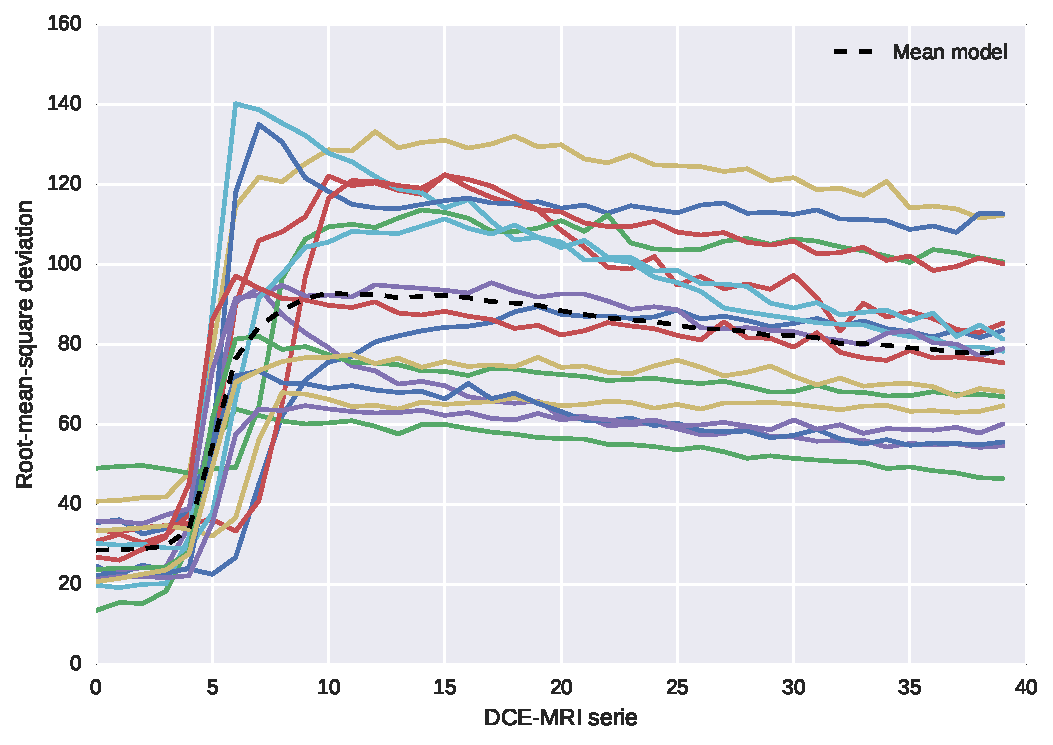
\includegraphics[width=.4\textwidth]{./images/DCE-normalization/rmse.pdf}}%
      \hfill%
      \subfigure[][\tiny Registered RMSD]{%
        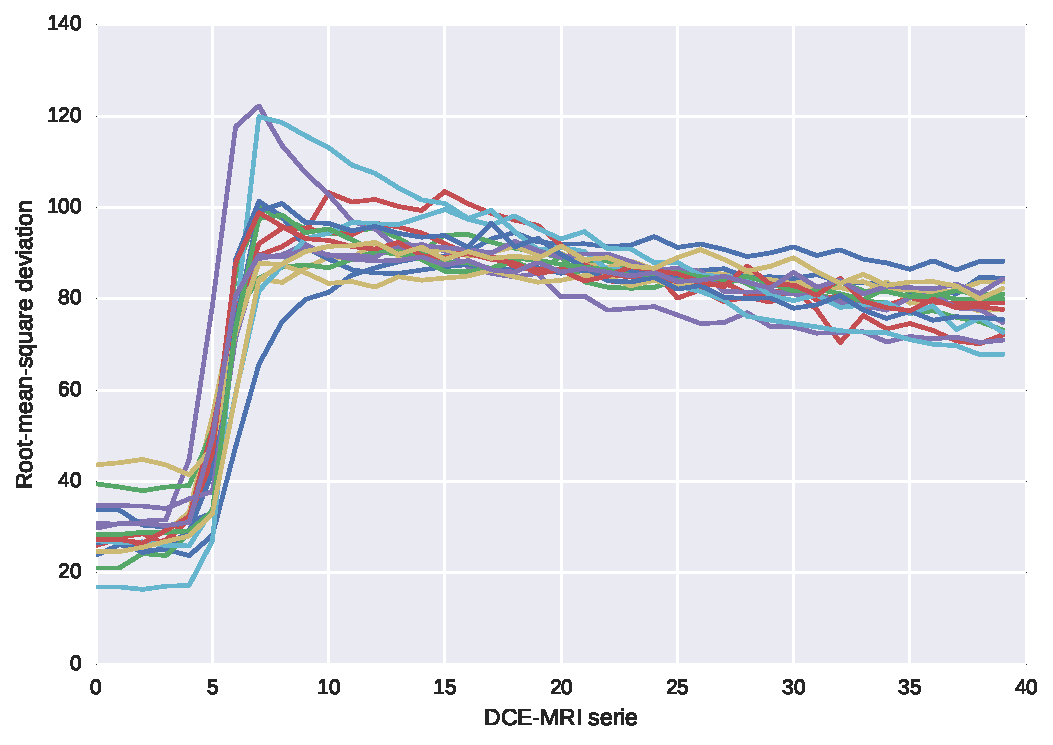
\includegraphics[width=.4\textwidth]{./images/DCE-normalization/rmse_aligned.pdf}}%
      \hspace*{\fill}%
    \end{figure}
  \end{block}
\end{frame}

\begin{frame}
  \frametitle{Toward a mp-MRI CAD for CaP}
  \framesubtitle{DCE-MRI normalization}
  \begin{block}{\small Evaluation through pharmacokinetic models}
    \begin{itemize}\scriptsize
    \item Brix's model
    \item Hoffmann's model
    \item Tofts' model
    \item PUN model
    \end{itemize}
  \end{block}
  \begin{block}{\small Other approaches}
    \begin{itemize}\scriptsize
    \item Semi-quantitative model
    \item Entire enhanced signal
    \end{itemize}
  \end{block}
  \begin{block}{\small Classification}
    \begin{itemize}\scriptsize
    \item Classification with random forest (RF)
    \item Leave-one-patient-out cross-validation (LOPO)
    \item Receiver operating characteristic (ROC) analysis
    \item Area under the ROC curve (AUC)
    \end{itemize}
  \end{block}
\end{frame}

\setcounter{subfigure}{0}% Reset subfigure counter

\begin{frame}
  \frametitle{Experiments}
  \framesubtitle{DCE-MRI normalization}
  \only<1>{
  \begin{block}{\small Quantitative and semi-quantitative models}
    \begin{figure}
      \includegraphics[width=.75\textwidth]{images/DCE-normalization/unormalized_methods_0.pdf}
      \caption{\tiny ROC analysis without normalization}
    \end{figure}
  \end{block}}
  \only<2>{
  \begin{block}{\small Quantitative and semi-quantitative models}
    \begin{figure}
      \includegraphics[width=.75\textwidth]{images/DCE-normalization/normalized_methods_0.pdf}
      \caption{\tiny ROC analysis with normalization}
    \end{figure}
  \end{block}}
\end{frame}

\begin{frame}
  \frametitle{Experiments}
  \framesubtitle{DCE-MRI normalization}
  \begin{block}{\small Entire signal}
    \begin{figure}
      \centering
      \includegraphics[width=.75\textwidth]{images/DCE-normalization/full_signal_0.pdf}
      \caption{\tiny ROC analysis with entire enhanced signal}
    \end{figure}
  \end{block}
\end{frame}

% \begin{frame}
%   \frametitle{Toward a mp-MRI CAD for CaP}
%   \framesubtitle{DCE Normalization}
%   \begin{block}{\small Mp-MRI CAD for CaP}
%     \begin{figure}
  \centering

  % Define block styles used later

  \tikzstyle{module}=[draw, draw=azulunam!80, text width=10em, 
  text centered, minimum height=5em, minimum width = 15em, drop shadow, rounded corners,
  fill=azulunam!30]
  \tikzstyle{moduleorange}=[draw, draw=orangeubfc!80, text width=10em, 
  text centered, minimum height=5em, minimum width = 15em, drop shadow, rounded corners,
  fill=orangeubfc!30]
  
  \tikzstyle{vecArrow} = [thick, decoration={markings,mark=at position
    1 with {\arrow[semithick]{open triangle 60}}},
  double distance=1.4pt, shorten >= 5.5pt,
  preaction = {decorate},
  postaction = {draw,line width=1.4pt, white,shorten >= 4.5pt}]

  % Define distances for bordering
  \def\blockdist{1.5}
  \def\edgedist{2.5}

  \begin{tikzpicture}[node distance=3cm,thick,scale=0.38, every node/.style={scale=0.38},path image/.style={
      path picture={
        \node at (path picture bounding box.center) {
          \includegraphics[width=1cm]{#1}
        };}}]
    \tikzstyle{conefill} = [path image=,fill opacity=0.8]
    \node[module=above:pre] (pre) at (4.5,-2.6) {\Large Pre-processing};
    \node[module,below of=pre] (seg) {\Large Segmentation};
    \node[module,below of=seg] (reg) {\Large Registration};

    \path[->,dashed] (seg.west) edge [bend right=70] node {} (reg.west);
    \path[->,dashed] (reg.east) edge [bend right=70] node {} (seg.east);

    \draw[->] (pre)--(seg);
    \draw[->] (seg)--(reg);

    \begin{pgfonlayer}{background}
      \path (pre.west |- pre.north)+(-0.9,1.0+\blockdist) node (a) {};
      \path (reg.east |- reg.south)+(+0.9,-0.5) node (b) {};
      
      \path[fill=azulunam!10,rounded corners, draw=azulunam!20, dashed] (a) rectangle (b);
    \end{pgfonlayer}
    
    \path (pre.north) +(0,+\blockdist) node (bgreg) {\Large Image regularization};

    \begin{scope}[node distance=10cm]
      \node[module] (det) [below right=0cm and 2cm of pre] {\Large Features detection};
    \end{scope}
    \begin{scope}[node distance=3.5cm]
      \node[module,above of=det] (roi) {\Large ROIs\\detection/selection};
    \end{scope}
    \node[module,below of=det] (sel) {\Large Data\\balancing};
    \node[module,below of=sel] (bal) {\Large Features\\selection/extraction};
    \node[module,below of=bal] (cla) {\Large Features\\classification/fusion};

    \draw[->] (roi)--(det);
    \draw[->] (det)--(sel);
    \draw[->] (sel)--(bal);
    \draw[->] (bal)--(cla);

    \begin{pgfonlayer}{background}
      \path (roi.west |- roi.north)+(-0.25,0.8) node (c) {};
      \path (roi.east |- roi.south)+(+0.25,-0.25) node (d) {};
      
      \path[fill=azulunam!20,rounded corners, draw=azulunam!25, dashed] (c) rectangle (d);
    \end{pgfonlayer}

    \path (roi.west |- roi.north) +(.75,0.4) node (bgfea) {\Large \textbf{CADe}};

    \begin{pgfonlayer}{background}
      \path (det.west |- det.north)+(-0.25,0.8) node (c) {};
      \path (cla.east |- cla.south)+(+0.25,-0.25) node (d) {};
      
      \path[fill=azulunam!20,rounded corners, draw=azulunam!25, dashed] (c) rectangle (d);
    \end{pgfonlayer}

    \path (roi.west |- det.north) +(.75,0.4) node (bgfea) {\Large \textbf{CADx}};     

    % \begin{scope}
    %   \transparent{0.6}\filldraw[fill=red!20!white,rounded corners,draw=red!25,dashed] (11.5,-8.7) rectangle (19,-9.8);
    % \end{scope}

    % Define the place where the arrow should start anf finish
    \path (seg.east |- seg.north)+(+1.15,0) node (e) {};
    \path (sel.west |- seg.north)+(-1.0,0) node (f) {};

    \draw[double distance =3pt,preaction={-triangle 90,thin,draw,shorten >=-1mm}] (e) -- (f) node[midway,above,above=.3em] {\large Regularized data};

    \begin{scope}[yshift=-33,xshift=-86]
      \transparent{0.6}\draw[path image=images/tikzimage/t2.eps] (0,0) rectangle (1.0,1.0);
    \end{scope}

    \begin{scope}[yshift=-36,xshift=-83]
      \transparent{0.6}\draw[path image=images/tikzimage/t2.eps] (0,0) rectangle (1.0,1.0);
    \end{scope}

    \begin{scope}[yshift=-39,xshift=-80]
      \transparent{0.8}\draw[path image=images/tikzimage/t2.eps] (0,0) rectangle (1.0,1.0);
      \path (0,0)+(-1.35,0.3) node {\Large T$_2$W-MRI};
    \end{scope}

    \begin{scope}[yshift=-100,xshift=-86]
      \transparent{0.6}\draw[path image=images/tikzimage/dce.eps] (0,0) rectangle (1.0,1.0);
    \end{scope}

    \begin{scope}[yshift=-103,xshift=-83]
      \transparent{0.6}\draw[path image=images/tikzimage/dce.eps] (0,0) rectangle (1.0,1.0);
    \end{scope}

    \begin{scope}[yshift=-106,xshift=-80]
      \transparent{0.8}\draw[path image=images/tikzimage/dce.eps] (0,0) rectangle (1.0,1.0);
      \path (0,0)+(-1.65,0.3) node {\Large DCE-MRI};
    \end{scope}

    \begin{scope}[yshift=-167,xshift=-86]
      \transparent{0.6}\draw[path image=images/tikzimage/dwi1.eps] (0,0) rectangle (1.0,1.0);
    \end{scope}

    \begin{scope}[yshift=-170,xshift=-83]
      \transparent{0.6}\draw[path image=images/tikzimage/dwi1.eps] (0,0) rectangle (1.0,1.0);
    \end{scope}

    \begin{scope}[yshift=-173,xshift=-80]
      \transparent{0.8}\draw[path image=images/tikzimage/dwi1.eps] (0,0) rectangle (1.0,1.0);
      \path (0,0)+(-1.65,0.3) node {\Large ADC};
    \end{scope}

    \begin{scope}[yshift=-234,xshift=-86]
      \transparent{0.6}\draw[path image=images/tikzimage/mrsi.eps] (0,0) rectangle (1.0,1.0);
    \end{scope}

    \begin{scope}[yshift=-237,xshift=-83]
      \transparent{0.6}\draw[path image=images/tikzimage/mrsi.eps] (0,0) rectangle (1.0,1.0);
    \end{scope}

    \begin{scope}[yshift=-240,xshift=-80]
      \transparent{0.8}\draw[path image=images/tikzimage/mrsi.eps] (0,0) rectangle (1.0,1.0);
      \path (0,0)+(-1.5,0.3) node {\Large MRSI};
    \end{scope}

    \path (pre.west |- roi.north)+(-2.5,-1.+\blockdist) node (g) {};
    \path (reg.west |- reg.south)+(-2.5,.5) node (h) {};

    \draw[decorate,decoration={brace,raise=2pt,amplitude=5pt}, thick]
    (g)--(h) ;
    
    \path (seg.west |- seg.north)+(-2.5,0) node (i) {};
    \path (seg.west |- seg.north)+(-0.9,0) node (j) {};
    
    % \draw[double distance =3pt,preaction={-triangle 90,thin,draw,shorten >=-1mm}] (i) -- (j);   

    \path (sel.east |- seg.north)+(2,0) node (k) {};
    \path (sel.east |- seg.north)+(0.5,0) node (l) {};
    
  \end{tikzpicture}
\end{figure}

%%% Local Variables: 
%%% mode: latex
%%% TeX-master: "../../presentation"
%%% End: 

%   \end{block}
% \end{frame}

% \subsection{Pre-processing}

% \begin{frame}
%   \frametitle{Toward a mp-MRI CAD for CaP}
%   \framesubtitle{Image regularization}
%   \begin{block}{\small Pre-processing}
%     \begin{figure}
  \centering

  % Define block styles used later

  \tikzstyle{module}=[draw, draw=azulunam!80, text width=10em, 
  text centered, minimum height=5em, minimum width = 15em, drop shadow, rounded corners,
  fill=azulunam!30]
  \tikzstyle{moduleorange}=[draw, draw=orangeubfc!80, text width=10em, 
  text centered, minimum height=5em, minimum width = 15em, drop shadow, rounded corners,
  fill=orangeubfc!30]
  
  \tikzstyle{vecArrow} = [thick, decoration={markings,mark=at position
    1 with {\arrow[semithick]{open triangle 60}}},
  double distance=1.4pt, shorten >= 5.5pt,
  preaction = {decorate},
  postaction = {draw,line width=1.4pt, white,shorten >= 4.5pt}]

  % Define distances for bordering
  \def\blockdist{1.5}
  \def\edgedist{2.5}

  \begin{tikzpicture}[node distance=3cm,thick,scale=0.3, every node/.style={scale=0.3},path image/.style={
      path picture={
        \node at (path picture bounding box.center) {
          \includegraphics[width=1cm]{#1}
        };}}]
    \tikzstyle{conefill} = [path image=,fill opacity=0.8]
    \node[moduleorange=above:pre] (pre) at (4.5,-2.6) {\Large Pre-processing};
    \node[module,below of=pre] (seg) {\Large Segmentation};
    \node[module,below of=seg] (reg) {\Large Registration};

    \path[->,dashed] (seg.west) edge [bend right=70] node {} (reg.west);
    \path[->,dashed] (reg.east) edge [bend right=70] node {} (seg.east);

    \draw[->] (pre)--(seg);
    \draw[->] (seg)--(reg);

    \begin{pgfonlayer}{background}
      \path (pre.west |- pre.north)+(-0.9,1.0+\blockdist) node (a) {};
      \path (reg.east |- reg.south)+(+0.9,-0.5) node (b) {};
      
      \path[fill=azulunam!10,rounded corners, draw=azulunam!20, dashed] (a) rectangle (b);
    \end{pgfonlayer}
    
    \path (pre.north) +(0,+\blockdist) node (bgreg) {\Large Image regularization};

    \begin{scope}[node distance=10cm]
      \node[module] (det) [below right=0cm and 2cm of pre] {\Large Features detection};
    \end{scope}
    \begin{scope}[node distance=3.5cm]
      \node[module,above of=det] (roi) {\Large ROIs\\detection/selection};
    \end{scope}
    \node[module,below of=det] (sel) {\Large Data\\balancing};
    \node[module,below of=sel] (bal) {\Large Features\\selection/extraction};
    \node[module,below of=bal] (cla) {\Large Features\\classification/fusion};

    \draw[->] (roi)--(det);
    \draw[->] (det)--(sel);
    \draw[->] (sel)--(bal);
    \draw[->] (bal)--(cla);

    \begin{pgfonlayer}{background}
      \path (roi.west |- roi.north)+(-0.25,0.8) node (c) {};
      \path (roi.east |- roi.south)+(+0.25,-0.25) node (d) {};
      
      \path[fill=azulunam!20,rounded corners, draw=azulunam!25, dashed] (c) rectangle (d);
    \end{pgfonlayer}

    \path (roi.west |- roi.north) +(.75,0.4) node (bgfea) {\Large \textbf{CADe}};

    \begin{pgfonlayer}{background}
      \path (det.west |- det.north)+(-0.25,0.8) node (c) {};
      \path (cla.east |- cla.south)+(+0.25,-0.25) node (d) {};
      
      \path[fill=azulunam!20,rounded corners, draw=azulunam!25, dashed] (c) rectangle (d);
    \end{pgfonlayer}

    \path (roi.west |- det.north) +(.75,0.4) node (bgfea) {\Large \textbf{CADx}};     

    % \begin{scope}
    %   \transparent{0.6}\filldraw[fill=red!20!white,rounded corners,draw=red!25,dashed] (11.5,-8.7) rectangle (19,-9.8);
    % \end{scope}

    % Define the place where the arrow should start anf finish
    \path (seg.east |- seg.north)+(+1.15,0) node (e) {};
    \path (sel.west |- seg.north)+(-1.0,0) node (f) {};

    \draw[double distance =3pt,preaction={-triangle 90,thin,draw,shorten >=-1mm}] (e) -- (f) node[midway,above,above=.3em] {\large Regularized data};

    \begin{scope}[yshift=-33,xshift=-86]
      \transparent{0.6}\draw[path image=images/tikzimage/t2.eps] (0,0) rectangle (1.0,1.0);
    \end{scope}

    \begin{scope}[yshift=-36,xshift=-83]
      \transparent{0.6}\draw[path image=images/tikzimage/t2.eps] (0,0) rectangle (1.0,1.0);
    \end{scope}

    \begin{scope}[yshift=-39,xshift=-80]
      \transparent{0.8}\draw[path image=images/tikzimage/t2.eps] (0,0) rectangle (1.0,1.0);
      \path (0,0)+(-1.35,0.3) node {\Large T$_2$W-MRI};
    \end{scope}

    \begin{scope}[yshift=-100,xshift=-86]
      \transparent{0.6}\draw[path image=images/tikzimage/dce.eps] (0,0) rectangle (1.0,1.0);
    \end{scope}

    \begin{scope}[yshift=-103,xshift=-83]
      \transparent{0.6}\draw[path image=images/tikzimage/dce.eps] (0,0) rectangle (1.0,1.0);
    \end{scope}

    \begin{scope}[yshift=-106,xshift=-80]
      \transparent{0.8}\draw[path image=images/tikzimage/dce.eps] (0,0) rectangle (1.0,1.0);
      \path (0,0)+(-1.65,0.3) node {\Large DCE-MRI};
    \end{scope}

    \begin{scope}[yshift=-167,xshift=-86]
      \transparent{0.6}\draw[path image=images/tikzimage/dwi1.eps] (0,0) rectangle (1.0,1.0);
    \end{scope}

    \begin{scope}[yshift=-170,xshift=-83]
      \transparent{0.6}\draw[path image=images/tikzimage/dwi1.eps] (0,0) rectangle (1.0,1.0);
    \end{scope}

    \begin{scope}[yshift=-173,xshift=-80]
      \transparent{0.8}\draw[path image=images/tikzimage/dwi1.eps] (0,0) rectangle (1.0,1.0);
      \path (0,0)+(-1.65,0.3) node {\Large ADC};
    \end{scope}

    \begin{scope}[yshift=-234,xshift=-86]
      \transparent{0.6}\draw[path image=images/tikzimage/mrsi.eps] (0,0) rectangle (1.0,1.0);
    \end{scope}

    \begin{scope}[yshift=-237,xshift=-83]
      \transparent{0.6}\draw[path image=images/tikzimage/mrsi.eps] (0,0) rectangle (1.0,1.0);
    \end{scope}

    \begin{scope}[yshift=-240,xshift=-80]
      \transparent{0.8}\draw[path image=images/tikzimage/mrsi.eps] (0,0) rectangle (1.0,1.0);
      \path (0,0)+(-1.5,0.3) node {\Large MRSI};
    \end{scope}

    \path (pre.west |- roi.north)+(-2.5,-1.+\blockdist) node (g) {};
    \path (reg.west |- reg.south)+(-2.5,.5) node (h) {};

    \draw[decorate,decoration={brace,raise=2pt,amplitude=5pt}, thick]
    (g)--(h) ;
    
    \path (seg.west |- seg.north)+(-2.5,0) node (i) {};
    \path (seg.west |- seg.north)+(-0.9,0) node (j) {};
    
    % \draw[double distance =3pt,preaction={-triangle 90,thin,draw,shorten >=-1mm}] (i) -- (j);   

    \path (sel.east |- seg.north)+(2,0) node (k) {};
    \path (sel.east |- seg.north)+(0.5,0) node (l) {};
    
  \end{tikzpicture}
\end{figure}

%%% Local Variables: 
%%% mode: latex
%%% TeX-master: "../../presentation"
%%% End: 

%   \end{block}
% \end{frame}

\subsubsection{Segmentation \& registration}

\begin{frame}
  \frametitle{Toward a mp-MRI CAD for CaP}
  \framesubtitle{Image regularization}
  \begin{block}{\small Segmentation \& registration}
    \begin{figure}
  \centering

  % Define block styles used later

  \tikzstyle{module}=[draw, draw=azulunam!80, text width=10em, 
  text centered, minimum height=5em, minimum width = 15em, drop shadow, rounded corners,
  fill=azulunam!30]
  \tikzstyle{moduleorange}=[draw, draw=orangeubfc!80, text width=10em, 
  text centered, minimum height=5em, minimum width = 15em, drop shadow, rounded corners,
  fill=orangeubfc!30]
  
  \tikzstyle{vecArrow} = [thick, decoration={markings,mark=at position
    1 with {\arrow[semithick]{open triangle 60}}},
  double distance=1.4pt, shorten >= 5.5pt,
  preaction = {decorate},
  postaction = {draw,line width=1.4pt, white,shorten >= 4.5pt}]

  % Define distances for bordering
  \def\blockdist{1.5}
  \def\edgedist{2.5}

  \begin{tikzpicture}[node distance=3cm,thick,scale=0.3, every node/.style={scale=0.3},path image/.style={
      path picture={
        \node at (path picture bounding box.center) {
          \includegraphics[width=1cm]{#1}
        };}}]
    \tikzstyle{conefill} = [path image=,fill opacity=0.8]
    \node[module=above:pre] (pre) at (4.5,-2.6) {\Large Pre-processing};
    \node[moduleorange,below of=pre] (seg) {\Large Segmentation};
    \node[moduleorange,below of=seg] (reg) {\Large Registration};

    \path[->,dashed] (seg.west) edge [bend right=70] node {} (reg.west);
    \path[->,dashed] (reg.east) edge [bend right=70] node {} (seg.east);

    \draw[->] (pre)--(seg);
    \draw[->] (seg)--(reg);

    \begin{pgfonlayer}{background}
      \path (pre.west |- pre.north)+(-0.9,1.0+\blockdist) node (a) {};
      \path (reg.east |- reg.south)+(+0.9,-0.5) node (b) {};
      
      \path[fill=azulunam!10,rounded corners, draw=azulunam!20, dashed] (a) rectangle (b);
    \end{pgfonlayer}
    
    \path (pre.north) +(0,+\blockdist) node (bgreg) {\Large Image regularization};

    \begin{scope}[node distance=10cm]
      \node[module] (det) [below right=0cm and 2cm of pre] {\Large Features detection};
    \end{scope}
    \begin{scope}[node distance=3.5cm]
      \node[module,above of=det] (roi) {\Large ROIs\\detection/selection};
    \end{scope}
    \node[module,below of=det] (sel) {\Large Data\\balancing};
    \node[module,below of=sel] (bal) {\Large Features\\selection/extraction};
    \node[module,below of=bal] (cla) {\Large Features\\classification/fusion};

    \draw[->] (roi)--(det);
    \draw[->] (det)--(sel);
    \draw[->] (sel)--(bal);
    \draw[->] (bal)--(cla);

    \begin{pgfonlayer}{background}
      \path (roi.west |- roi.north)+(-0.25,0.8) node (c) {};
      \path (roi.east |- roi.south)+(+0.25,-0.25) node (d) {};
      
      \path[fill=azulunam!20,rounded corners, draw=azulunam!25, dashed] (c) rectangle (d);
    \end{pgfonlayer}

    \path (roi.west |- roi.north) +(.75,0.4) node (bgfea) {\Large \textbf{CADe}};

    \begin{pgfonlayer}{background}
      \path (det.west |- det.north)+(-0.25,0.8) node (c) {};
      \path (cla.east |- cla.south)+(+0.25,-0.25) node (d) {};
      
      \path[fill=azulunam!20,rounded corners, draw=azulunam!25, dashed] (c) rectangle (d);
    \end{pgfonlayer}

    \path (roi.west |- det.north) +(.75,0.4) node (bgfea) {\Large \textbf{CADx}};     

    % \begin{scope}
    %   \transparent{0.6}\filldraw[fill=red!20!white,rounded corners,draw=red!25,dashed] (11.5,-8.7) rectangle (19,-9.8);
    % \end{scope}

    % Define the place where the arrow should start anf finish
    \path (seg.east |- seg.north)+(+1.15,0) node (e) {};
    \path (sel.west |- seg.north)+(-1.0,0) node (f) {};

    \draw[double distance =3pt,preaction={-triangle 90,thin,draw,shorten >=-1mm}] (e) -- (f) node[midway,above,above=.3em] {\large Regularized data};

    \begin{scope}[yshift=-33,xshift=-86]
      \transparent{0.6}\draw[path image=images/tikzimage/t2.eps] (0,0) rectangle (1.0,1.0);
    \end{scope}

    \begin{scope}[yshift=-36,xshift=-83]
      \transparent{0.6}\draw[path image=images/tikzimage/t2.eps] (0,0) rectangle (1.0,1.0);
    \end{scope}

    \begin{scope}[yshift=-39,xshift=-80]
      \transparent{0.8}\draw[path image=images/tikzimage/t2.eps] (0,0) rectangle (1.0,1.0);
      \path (0,0)+(-1.35,0.3) node {\Large T$_2$W-MRI};
    \end{scope}

    \begin{scope}[yshift=-100,xshift=-86]
      \transparent{0.6}\draw[path image=images/tikzimage/dce.eps] (0,0) rectangle (1.0,1.0);
    \end{scope}

    \begin{scope}[yshift=-103,xshift=-83]
      \transparent{0.6}\draw[path image=images/tikzimage/dce.eps] (0,0) rectangle (1.0,1.0);
    \end{scope}

    \begin{scope}[yshift=-106,xshift=-80]
      \transparent{0.8}\draw[path image=images/tikzimage/dce.eps] (0,0) rectangle (1.0,1.0);
      \path (0,0)+(-1.65,0.3) node {\Large DCE-MRI};
    \end{scope}

    \begin{scope}[yshift=-167,xshift=-86]
      \transparent{0.6}\draw[path image=images/tikzimage/dwi1.eps] (0,0) rectangle (1.0,1.0);
    \end{scope}

    \begin{scope}[yshift=-170,xshift=-83]
      \transparent{0.6}\draw[path image=images/tikzimage/dwi1.eps] (0,0) rectangle (1.0,1.0);
    \end{scope}

    \begin{scope}[yshift=-173,xshift=-80]
      \transparent{0.8}\draw[path image=images/tikzimage/dwi1.eps] (0,0) rectangle (1.0,1.0);
      \path (0,0)+(-1.65,0.3) node {\Large ADC};
    \end{scope}

    \begin{scope}[yshift=-234,xshift=-86]
      \transparent{0.6}\draw[path image=images/tikzimage/mrsi.eps] (0,0) rectangle (1.0,1.0);
    \end{scope}

    \begin{scope}[yshift=-237,xshift=-83]
      \transparent{0.6}\draw[path image=images/tikzimage/mrsi.eps] (0,0) rectangle (1.0,1.0);
    \end{scope}

    \begin{scope}[yshift=-240,xshift=-80]
      \transparent{0.8}\draw[path image=images/tikzimage/mrsi.eps] (0,0) rectangle (1.0,1.0);
      \path (0,0)+(-1.5,0.3) node {\Large MRSI};
    \end{scope}

    \path (pre.west |- roi.north)+(-2.5,-1.+\blockdist) node (g) {};
    \path (reg.west |- reg.south)+(-2.5,.5) node (h) {};

    \draw[decorate,decoration={brace,raise=2pt,amplitude=5pt}, thick]
    (g)--(h) ;
    
    \path (seg.west |- seg.north)+(-2.5,0) node (i) {};
    \path (seg.west |- seg.north)+(-0.9,0) node (j) {};
    
    % \draw[double distance =3pt,preaction={-triangle 90,thin,draw,shorten >=-1mm}] (i) -- (j);   

    \path (sel.east |- seg.north)+(2,0) node (k) {};
    \path (sel.east |- seg.north)+(0.5,0) node (l) {};
    
  \end{tikzpicture}
\end{figure}

%%% Local Variables: 
%%% mode: latex
%%% TeX-master: "../../presentation"
%%% End: 

  \end{block}
\end{frame}

\begin{frame}
  \frametitle{Toward a mp-MRI CAD for CaP}
  \framesubtitle{Segmentation \& registration}
  \begin{block}{\small Resampling}
    \begin{itemize}\scriptsize
    \item ADC and DCE-MRI are resampled to the T$_2$W-MRI resolution
    \end{itemize}
  \end{block}
  \begin{block}{\small Segmentation}
    \begin{itemize}\scriptsize
    \item Manual prostate segmentation available for T$_2$W-MRI, DCE-MRI, and ADC
    \item CaP, PZ, and CG manual segmentation available for T$_2$W-MRI
    \end{itemize}
  \end{block}
  \begin{block}{\small Registration}
    \begin{itemize}\scriptsize
    \item Intra-patient motions correction in DCE-MRI: rigid registration using mutual information
    \item DCE-MRI is registered to T$_2$W-MRI using the prostate segmentation
    \item ADC is registered to T$_2$W-MRI using the prostate segmentation
    \end{itemize}
  \end{block}
\end{frame}

\subsection{CADe-CADx}

\begin{frame}
  \frametitle{Toward a mp-MRI CAD for CaP}
  \framesubtitle{CADe-CADx}
  \begin{block}{\small Summary of experiments}
    \begin{itemize}\scriptsize
    \item Investigate the performance of features from each standalone modality
    \item Investigate the performance of the combination of features: \emph{coarse combination}
    \item Investigate the effect of data balancing
    \item Investigate the effect of selection/extraction
    \item Investigate the performance of the combination of features: \emph{fine-tuned combination}
    \end{itemize}
  \end{block}
\end{frame}

\subsubsection{Features detection}

\begin{frame}
  \frametitle{Toward a mp-MRI CAD for CaP}
  \framesubtitle{CADe-CADx}
  \begin{block}{\small Features detection}
    \begin{figure}
  \centering

  % Define block styles used later

  \tikzstyle{module}=[draw, draw=azulunam!80, text width=10em, 
  text centered, minimum height=5em, minimum width = 15em, drop shadow, rounded corners,
  fill=azulunam!30]
  \tikzstyle{moduleorange}=[draw, draw=orangeubfc!80, text width=10em, 
  text centered, minimum height=5em, minimum width = 15em, drop shadow, rounded corners,
  fill=orangeubfc!30]
  
  \tikzstyle{vecArrow} = [thick, decoration={markings,mark=at position
    1 with {\arrow[semithick]{open triangle 60}}},
  double distance=1.4pt, shorten >= 5.5pt,
  preaction = {decorate},
  postaction = {draw,line width=1.4pt, white,shorten >= 4.5pt}]

  % Define distances for bordering
  \def\blockdist{1.5}
  \def\edgedist{2.5}

  \begin{tikzpicture}[node distance=3cm,thick,scale=0.38, every node/.style={scale=0.38},path image/.style={
      path picture={
        \node at (path picture bounding box.center) {
          \includegraphics[width=1cm]{#1}
        };}}]
    \tikzstyle{conefill} = [path image=,fill opacity=0.8]
    \node[module=above:pre] (pre) at (4.5,-2.6) {\Large Pre-processing};
    \node[module,below of=pre] (seg) {\Large Segmentation};
    \node[module,below of=seg] (reg) {\Large Registration};

    \path[->,dashed] (seg.west) edge [bend right=70] node {} (reg.west);
    \path[->,dashed] (reg.east) edge [bend right=70] node {} (seg.east);

    \draw[->] (pre)--(seg);
    \draw[->] (seg)--(reg);

    \begin{pgfonlayer}{background}
      \path (pre.west |- pre.north)+(-0.9,1.0+\blockdist) node (a) {};
      \path (reg.east |- reg.south)+(+0.9,-0.5) node (b) {};
      
      \path[fill=azulunam!10,rounded corners, draw=azulunam!20, dashed] (a) rectangle (b);
    \end{pgfonlayer}
    
    \path (pre.north) +(0,+\blockdist) node (bgreg) {\Large Image regularization};

    \begin{scope}[node distance=10cm]
      \node[moduleorange] (det) [below right=0cm and 2cm of pre] {\Large Features detection};
    \end{scope}
    \begin{scope}[node distance=3.5cm]
      \node[module,above of=det] (roi) {\Large ROIs\\detection/selection};
    \end{scope}
    %\node[module,below of=det] (sel) {\Large Data\\balancing};
    %\node[module,below of=sel] (bal) {\Large Features\\selection/extraction};
    \node[moduleorange,below of=det] (cla) {\Large Features\\classification/fusion};

    \draw[->] (roi)--(det);
    %\draw[->] (det)--(sel);
    %\draw[->] (sel)--(bal);
    \draw[->] (det)--(cla);

    \begin{pgfonlayer}{background}
      \path (roi.west |- roi.north)+(-0.25,0.8) node (c) {};
      \path (roi.east |- roi.south)+(+0.25,-0.25) node (d) {};
      
      \path[fill=azulunam!20,rounded corners, draw=azulunam!25, dashed] (c) rectangle (d);
    \end{pgfonlayer}

    \path (roi.west |- roi.north) +(.75,0.4) node (bgfea) {\Large \textbf{CADe}};

    \begin{pgfonlayer}{background}
      \path (det.west |- det.north)+(-0.25,0.8) node (c) {};
      \path (cla.east |- cla.south)+(+0.25,-0.25) node (d) {};
      
      \path[fill=azulunam!20,rounded corners, draw=azulunam!25, dashed] (c) rectangle (d);
    \end{pgfonlayer}

    \path (roi.west |- det.north) +(.75,0.4) node (bgfea) {\Large \textbf{CADx}};     

    % \begin{scope}
    %   \transparent{0.6}\filldraw[fill=red!20!white,rounded corners,draw=red!25,dashed] (11.5,-8.7) rectangle (19,-9.8);
    % \end{scope}

    % Define the place where the arrow should start anf finish
    \path (seg.east |- seg.north)+(+1.15,0) node (e) {};
    \path (sel.west |- seg.north)+(-1.0,0) node (f) {};

    \draw[double distance =3pt,preaction={-triangle 90,thin,draw,shorten >=-1mm}] (e) -- (f) node[midway,above,above=.3em] {\large Regularized data};

    \begin{scope}[yshift=-33,xshift=-86]
      \transparent{0.6}\draw[path image=images/tikzimage/t2.eps] (0,0) rectangle (1.0,1.0);
    \end{scope}

    \begin{scope}[yshift=-36,xshift=-83]
      \transparent{0.6}\draw[path image=images/tikzimage/t2.eps] (0,0) rectangle (1.0,1.0);
    \end{scope}

    \begin{scope}[yshift=-39,xshift=-80]
      \transparent{0.8}\draw[path image=images/tikzimage/t2.eps] (0,0) rectangle (1.0,1.0);
      \path (0,0)+(-1.35,0.3) node {\Large T$_2$W-MRI};
    \end{scope}

    \begin{scope}[yshift=-100,xshift=-86]
      \transparent{0.6}\draw[path image=images/tikzimage/dce.eps] (0,0) rectangle (1.0,1.0);
    \end{scope}

    \begin{scope}[yshift=-103,xshift=-83]
      \transparent{0.6}\draw[path image=images/tikzimage/dce.eps] (0,0) rectangle (1.0,1.0);
    \end{scope}

    \begin{scope}[yshift=-106,xshift=-80]
      \transparent{0.8}\draw[path image=images/tikzimage/dce.eps] (0,0) rectangle (1.0,1.0);
      \path (0,0)+(-1.65,0.3) node {\Large DCE-MRI};
    \end{scope}

    \begin{scope}[yshift=-167,xshift=-86]
      \transparent{0.6}\draw[path image=images/tikzimage/dwi1.eps] (0,0) rectangle (1.0,1.0);
    \end{scope}

    \begin{scope}[yshift=-170,xshift=-83]
      \transparent{0.6}\draw[path image=images/tikzimage/dwi1.eps] (0,0) rectangle (1.0,1.0);
    \end{scope}

    \begin{scope}[yshift=-173,xshift=-80]
      \transparent{0.8}\draw[path image=images/tikzimage/dwi1.eps] (0,0) rectangle (1.0,1.0);
      \path (0,0)+(-1.65,0.3) node {\Large ADC};
    \end{scope}

    \begin{scope}[yshift=-234,xshift=-86]
      \transparent{0.6}\draw[path image=images/tikzimage/mrsi.eps] (0,0) rectangle (1.0,1.0);
    \end{scope}

    \begin{scope}[yshift=-237,xshift=-83]
      \transparent{0.6}\draw[path image=images/tikzimage/mrsi.eps] (0,0) rectangle (1.0,1.0);
    \end{scope}

    \begin{scope}[yshift=-240,xshift=-80]
      \transparent{0.8}\draw[path image=images/tikzimage/mrsi.eps] (0,0) rectangle (1.0,1.0);
      \path (0,0)+(-1.5,0.3) node {\Large MRSI};
    \end{scope}

    \path (pre.west |- roi.north)+(-2.5,-1.+\blockdist) node (g) {};
    \path (reg.west |- reg.south)+(-2.5,.5) node (h) {};

    \draw[decorate,decoration={brace,raise=2pt,amplitude=5pt}, thick]
    (g)--(h) ;
    
    \path (seg.west |- seg.north)+(-2.5,0) node (i) {};
    \path (seg.west |- seg.north)+(-0.9,0) node (j) {};
    
    % \draw[double distance =3pt,preaction={-triangle 90,thin,draw,shorten >=-1mm}] (i) -- (j);   

    \path (sel.east |- seg.north)+(2,0) node (k) {};
    \path (sel.east |- seg.north)+(0.5,0) node (l) {};
    
  \end{tikzpicture}
\end{figure}

%%% Local Variables: 
%%% mode: latex
%%% TeX-master: "../../presentation"
%%% End: 

  \end{block}
\end{frame}

\begin{frame}
  \frametitle{Toward a mp-MRI CAD for CaP}
  \framesubtitle{Feature detection}
  \begin{columns}
    \begin{column}{0.65\textwidth}
      \begin{block}{\small T$_2$W-MRI and ADC features}
        \begin{columns}
          \begin{column}{0.45\textwidth}
            \begin{itemize}\scriptsize
            \item Intensity
            \item Kirsch filter
            \item Laplacian filter*
            \item Prewitt filter*
            \item Scharr filter*
            \item Sobel filter*
            \end{itemize}
          \end{column}
          \begin{column}{0.45\textwidth}
            \begin{itemize}\scriptsize
            \item DCT decomposition*
            \item Gabor filters*
            \item Phase congruency filter
            \item Haralick filter*
            \item LBP filter*
            \end{itemize}
          \end{column}
        \end{columns}
      \end{block}
    \end{column}
    \begin{column}{0.35\textwidth}
      \begin{block}{\small DCE-MRI features}
        \begin{itemize}\scriptsize
        \item Brix's model
        \item Hoffmann's model
        \item Tofts' model
        \item PUN model
        \item Semi-quantitative model
        \item Entire enhanced signal
        \end{itemize}
      \end{block}
    \end{column}
  \end{columns}
  \begin{columns}
    \begin{column}{0.65\textwidth}
      \begin{block}{\small MRSI features}
        \begin{itemize}\scriptsize
        \item Quantification with fixed bounds
        \item Quantification by fitting some modeled signal
        \item Entire spectra
        \end{itemize}
      \end{block}
    \end{column}
    \begin{column}{0.35\textwidth}
      \begin{block}{\small Spatial information}
        \begin{itemize}\scriptsize
        \item Relative distance
        \item Relative position
        \item Prostate zone
        \end{itemize}
      \end{block}
    \end{column}
  \end{columns}
  \vspace*{.3cm}
  \rule{4cm}{0.4pt} \\ \vspace*{-.2cm}
  {\noindent \tiny *These features are extracted using the 3D information}
\end{frame}

% \begin{frame}
%   \frametitle{Toward a mp-MRI CAD for CaP}
%   \framesubtitle{Anatomical features}
%   \begin{block}{\small Metrics\footnotemark,\footnotemark}
%     \begin{itemize}\scriptsize
%     \item Relative distance to the \emph{prostate boundary}
%     \item Relative distance to the \emph{prostate center}
%     \item Relative position in the \emph{Euclidean} coordinate systems
%     \item Relative position in the \emph{cylindrical} coordinate systems
%     \end{itemize}
%   \end{block}
%   \addtocounter{footnote}{-2}
%   \stepcounter{footnote} \footcitetext{Chen2008}
%   \stepcounter{footnote} \footcitetext{Litjens2014}
% \end{frame}


% \setcounter{subfigure}{0}% Reset subfigure counter

% \begin{frame}
%   \frametitle{Toward a mp-MRI CAD for CaP}
%   \framesubtitle{DCE-MRI}
%   \begin{block}{\small Quantitative and semi-quantitative models}
%     \begin{itemize}\scriptsize
%     \item Brix's model
%     \item Hoffmann's model
%     \item Tofts' model
%     \item PUN model
%     \item Semi-quantitative model
%     \item Entire enhanced signal
%     \end{itemize}
%   \end{block}
%   \begin{block}{\small Segmentation of arterial input function (AIF)}
%     \begin{figure}%
%       \centering
%       \hspace*{\fill}%
%       \subfigure[][\tiny Original]{%
%         \includegraphics[width=.3\textwidth]{./images/DCE-normalization/original.pdf}}%
%       \hfill%
%       \subfigure[][\tiny Candidate]{%
%         \includegraphics[width=.3\textwidth]{./images/DCE-normalization/candidate.pdf}}%
%       \hfill%
%       \subfigure[][\tiny AIF]{%
%         \includegraphics[width=.3\textwidth]{./images/DCE-normalization/aif.pdf}}%
%       \hspace*{\fill}%
%     \end{figure}
%     \vspace*{-.7cm}
%     \begin{itemize}\scriptsize
%     \item[(i)] K-means clustering with $k=6$
%     \item[(ii)] Select the cluster with the highest $90^{\text{th}}$ percentile
%     \item[(iii)] Select regions with an eccentricity $\mathcal{E} < 0.5$ and an area $\mathcal{A} \in [100, 400]$
%     \end{itemize}
%   \end{block}
% \end{frame}

% \begin{frame}
%   \frametitle{Toward a mp-MRI CAD for CaP}
%   \framesubtitle{MRSI}
%   \only<1>{
%     \begin{block}{\small Quantification strategies}
%       \begin{columns}
%         \begin{column}{.5\textwidth}
%           \begin{itemize}\scriptsize
%           \item<1-> Quantification with fixed bounds
%           \item<2-> Quantification by fitting some modeled signal
%           \item<4-> Entire spectra
%           \end{itemize}
%         \end{column}
%         \begin{column}{.5\textwidth}
%           \only<1>{
%             \begin{figure}%
%               \hspace*{-1.cm}
%               \includegraphics[width=1.\textwidth]{./images/mrsi/mrsi_healthy.eps}
%             \end{figure}}
%           \only<2>{
%             \begin{figure}%
%               \hspace*{-1.cm}
%               \includegraphics[width=1.\textwidth]{./images/meta_fitting.pdf}
%             \end{figure}}
%         \end{column}
%       \end{columns}
%     \end{block}}
%   \only<2>{
%     \begin{block}{\small Quantification strategies}
%       \begin{columns}
%         \begin{column}{.5\textwidth}
%           \begin{itemize}\scriptsize
%           \item<1-> Quantification with fixed bounds
%           \item<2-> Quantification by fitting some modeled signal
%           \item<4-> Entire spectra
%           \end{itemize}
%         \end{column}
%         \begin{column}{.5\textwidth}
%           \only<1>{
%             \begin{figure}%
%               \hspace*{-1.cm}
%               \includegraphics[width=1.\textwidth]{./images/mrsi/mrsi_healthy.eps}
%             \end{figure}}
%           \only<2>{
%             \begin{figure}%
%               \hspace*{-1.cm}
%               \includegraphics[width=1.\textwidth]{./images/meta_fitting.pdf}
%             \end{figure}}
%         \end{column}
%       \end{columns}
%     \end{block}}
%   \only<4>{
%     \begin{block}{\small Quantification strategies}
%       \begin{columns}
%         \begin{column}{.5\textwidth}
%           \begin{itemize}\scriptsize
%           \item<1-> Quantification with fixed bounds
%           \item<2-> Quantification by fitting some modeled signal
%           \item<4-> Entire spectra
%           \end{itemize}
%         \end{column}
%         \begin{column}{.5\textwidth}
%           \only<1>{
%             \begin{figure}%
%               \hspace*{-1.cm}
%               \includegraphics[width=1.\textwidth]{./images/mrsi/mrsi_healthy.eps}
%             \end{figure}}
%           \only<2>{
%             \begin{figure}%
%               \hspace*{-1.cm}
%               \includegraphics[width=1.\textwidth]{./images/meta_fitting.pdf}
%             \end{figure}}
%           \only<4>{
%             \begin{figure}%
%               \hspace*{-1.cm}
%               \includegraphics[width=1.\textwidth]{./images/meta_fitting.pdf}
%             \end{figure}}
%         \end{column}
%       \end{columns}
%     \end{block}}
%   \only<1>{
%     \begin{block}{\small Assumptions}
%       \begin{itemize}\scriptsize
%       \item Integrate citrate from \SIrange{2.46}{2.82}{\ppm}
%       \item Integrate choline from \SIrange{3.19}{3.23}{\ppm}
%       \end{itemize}
%     \end{block}}
%   \only<3>{
%     \begin{block}{\small Citrate quantification}
%       \begin{equation}\tiny
%         \begin{aligned}
%           & \argmin_{\mathbf{w}} 
%           & & | S(x) - M_1(x; \mathbf{w}) |^{2} \ , \label{eq:mincostcit} \\
%           & \text{subject to}
%           & & 2.54 < \mu < 2.68 \ , \\
%           &&& 0.06 < \delta_1, \delta_2 < 0.16 \ , \\
%           &&& 0.01 < \sigma_1, \sigma_2, \sigma_3 < 0.1 \ , \\
%           &&& \alpha_1, \alpha_2, \alpha_3 > 0 \ .
%         \end{aligned}
%       \end{equation}
%       \begin{equation}\tiny
%         M_1(x; \mathbf{w}) = \alpha_1 \mathcal{N}(x; \mu, \sigma_1) + \alpha_2 \mathcal{N}(x; \mu + \delta_2, \sigma_2) + \alpha_3 \mathcal{N}(x; \mu - \delta_3, \sigma_3) \ .
%         \label{eq:costcit}
%       \end{equation}
%     \end{block}
%     \begin{block}{\small Choline quantification}
%       \begin{equation}\tiny
%         \begin{aligned}
%           & \argmin_{\mathbf{\mu, \sigma}} 
%           & & | S(x) - M_2(x; \mu, \sigma) |^{2} \ , \label{eq:mincostcho} \\
%           & \text{subject to}
%           & & 3.17 < \mu < 3.21 \ , \\
%           &&& 0.001 < \sigma < 0.02 \ , \\
%           &&& \alpha > 0 \ .
%         \end{aligned}
%       \end{equation}
%       \begin{equation}\tiny
%         M_2(x; \mu, \sigma) = \alpha \mathcal{N}(x; \mu, \sigma) \ .
%         \label{eq:costcho}
%       \end{equation}
%     \end{block}}
% \end{frame}

% \subsubsection{Features classification}

\begin{frame}
  \frametitle{Toward a mp-MRI CAD for CaP}
  \framesubtitle{CADe-CADx}
  \begin{block}{\small Features classification}
    \begin{figure}
  \centering

  % Define block styles used later

  \tikzstyle{module}=[draw, draw=azulunam!80, text width=15em, 
  text centered, minimum height=5em, minimum width = 15em, drop shadow, rounded corners,
  fill=azulunam!30]
  \tikzstyle{moduleorange}=[draw, draw=orangeubfc!80, text width=15em, 
  text centered, minimum height=5em, minimum width = 15em, drop shadow, rounded corners,
  fill=orangeubfc!30]
  
  \tikzstyle{vecArrow} = [thick, decoration={markings,mark=at position
    1 with {\arrow[semithick]{open triangle 60}}},
  double distance=1.4pt, shorten >= 5.5pt,
  preaction = {decorate},
  postaction = {draw,line width=1.4pt, white,shorten >= 4.5pt}]

  % Define distances for bordering
  \def\blockdist{1.5}
  \def\edgedist{2.5}

  \begin{tikzpicture}[node distance=3cm,thick,scale=0.38, every node/.style={scale=0.38},path image/.style={
      path picture={
        \node at (path picture bounding box.center) {
          \includegraphics[width=1cm]{#1}
        };}}]
    \tikzstyle{conefill} = [path image=,fill opacity=0.8]
    \node[module=above:pre] (pre) at (4.5,-2.6) {\Large \textbf{Pre-processing}};
    \node[module,below of=pre] (seg) {\Large \textbf{Segmentation}};
    \node[module,below of=seg] (reg) {\Large \textbf{Registration}};

    \path[->,dashed] (seg.west) edge [bend right=70] node {} (reg.west);
    \path[->,dashed] (reg.east) edge [bend right=70] node {} (seg.east);

    \draw[->] (pre)--(seg);
    \draw[->] (seg)--(reg);

    \begin{pgfonlayer}{background}
      \path (pre.west |- pre.north)+(-0.9,1.0+\blockdist) node (a) {};
      \path (reg.east |- reg.south)+(+0.9,-0.5) node (b) {};
      
      \path[fill=azulunam!10,rounded corners, draw=azulunam!20, dashed] (a) rectangle (b);
    \end{pgfonlayer}
    
    \path (pre.north) +(0,+\blockdist) node (bgreg) {\Large \textbf{Image regularization}};

    \begin{scope}[node distance=10cm]
      \node[module] (det) [below right=0cm and 2cm of pre] {\Large \textbf{Features detection}};
    \end{scope}
    \begin{scope}[node distance=3.5cm]
      \node[module,above of=det] (roi) {\Large \textbf{ROIs\\detection/selection}};
    \end{scope}
    \node[module,below of=det] (sel) {\Large \textbf{Data\\balancing}};
    \node[module,below of=sel] (bal) {\Large \textbf{Features\\selection/extraction}};
    \node[moduleorange,below of=bal] (cla) {\Large \textbf{Features\\classification}};

    \draw[->] (roi)--(det);
    \draw[->] (det)--(sel);
    \draw[->] (sel)--(bal);
    \draw[->] (bal)--(cla);

    \begin{pgfonlayer}{background}
      \path (roi.west |- roi.north)+(-0.25,0.8) node (c) {};
      \path (roi.east |- roi.south)+(+0.25,-0.25) node (d) {};
      
      \path[fill=azulunam!20,rounded corners, draw=azulunam!25, dashed] (c) rectangle (d);
    \end{pgfonlayer}

    \path (roi.west |- roi.north) +(.75,0.4) node (bgfea) {\Large \textbf{CADe}};

    \begin{pgfonlayer}{background}
      \path (det.west |- det.north)+(-0.25,0.8) node (c) {};
      \path (cla.east |- cla.south)+(+0.25,-0.25) node (d) {};
      
      \path[fill=azulunam!20,rounded corners, draw=azulunam!25, dashed] (c) rectangle (d);
    \end{pgfonlayer}

    \path (roi.west |- det.north) +(.75,0.4) node (bgfea) {\Large \textbf{CADx}};     

    % \begin{scope}
    %   \transparent{0.6}\filldraw[fill=red!20!white,rounded corners,draw=red!25,dashed] (11.5,-8.7) rectangle (19,-9.8);
    % \end{scope}

    % Define the place where the arrow should start anf finish
    \path (seg.east |- seg.north)+(+1.15,0) node (e) {};
    \path (sel.west |- seg.north)+(-1.0,0) node (f) {};

    \draw[double distance =3pt,preaction={-triangle 90,thin,draw,shorten >=-1mm}] (e) -- (f) node[midway,above,above=.3em] {\large \textbf{Regularized data}};

    \begin{scope}[yshift=-33,xshift=-86]
      \transparent{0.6}\draw[path image=images/tikzimage/t2.eps] (0,0) rectangle (1.0,1.0);
    \end{scope}

    \begin{scope}[yshift=-36,xshift=-83]
      \transparent{0.6}\draw[path image=images/tikzimage/t2.eps] (0,0) rectangle (1.0,1.0);
    \end{scope}

    \begin{scope}[yshift=-39,xshift=-80]
      \transparent{0.8}\draw[path image=images/tikzimage/t2.eps] (0,0) rectangle (1.0,1.0);
      \path (0,0)+(-1.65,0.3) node {\Large \textbf{T$_2$W-MRI}};
    \end{scope}

    \begin{scope}[yshift=-100,xshift=-86]
      \transparent{0.6}\draw[path image=images/tikzimage/dce.eps] (0,0) rectangle (1.0,1.0);
    \end{scope}

    \begin{scope}[yshift=-103,xshift=-83]
      \transparent{0.6}\draw[path image=images/tikzimage/dce.eps] (0,0) rectangle (1.0,1.0);
    \end{scope}

    \begin{scope}[yshift=-106,xshift=-80]
      \transparent{0.8}\draw[path image=images/tikzimage/dce.eps] (0,0) rectangle (1.0,1.0);
      \path (0,0)+(-1.65,0.3) node {\Large \textbf{DCE-MRI}};
    \end{scope}

    \begin{scope}[yshift=-167,xshift=-86]
      \transparent{0.6}\draw[path image=images/tikzimage/dwi1.eps] (0,0) rectangle (1.0,1.0);
    \end{scope}

    \begin{scope}[yshift=-170,xshift=-83]
      \transparent{0.6}\draw[path image=images/tikzimage/dwi1.eps] (0,0) rectangle (1.0,1.0);
    \end{scope}

    \begin{scope}[yshift=-173,xshift=-80]
      \transparent{0.8}\draw[path image=images/tikzimage/dwi1.eps] (0,0) rectangle (1.0,1.0);
      \path (0,0)+(-1.65,0.3) node {\Large \textbf{ADC}};
    \end{scope}

    \begin{scope}[yshift=-234,xshift=-86]
      \transparent{0.6}\draw[path image=images/tikzimage/mrsi.eps] (0,0) rectangle (1.0,1.0);
    \end{scope}

    \begin{scope}[yshift=-237,xshift=-83]
      \transparent{0.6}\draw[path image=images/tikzimage/mrsi.eps] (0,0) rectangle (1.0,1.0);
    \end{scope}

    \begin{scope}[yshift=-240,xshift=-80]
      \transparent{0.8}\draw[path image=images/tikzimage/mrsi.eps] (0,0) rectangle (1.0,1.0);
      \path (0,0)+(-1.5,0.3) node {\Large \textbf{MRSI}};
    \end{scope}

    \path (pre.west |- roi.north)+(-2.5,-1.+\blockdist) node (g) {};
    \path (reg.west |- reg.south)+(-2.5,.5) node (h) {};

    \draw[decorate,decoration={brace,raise=2pt,amplitude=5pt}, thick]
    (g)--(h) ;
    
    \path (seg.west |- seg.north)+(-2.5,0) node (i) {};
    \path (seg.west |- seg.north)+(-0.9,0) node (j) {};
    
    % \draw[double distance =3pt,preaction={-triangle 90,thin,draw,shorten >=-1mm}] (i) -- (j);   

    \path (sel.east |- seg.north)+(2,0) node (k) {};
    \path (sel.east |- seg.north)+(0.5,0) node (l) {};
    
  \end{tikzpicture}
\end{figure}

%%% Local Variables: 
%%% mode: latex
%%% TeX-master: "../../presentation"
%%% End: 

  \end{block}
\end{frame}

\begin{frame}
  \frametitle{Toward a mp-MRI CAD for CaP}
  \framesubtitle{Features classification}
  \begin{columns}
    \begin{column}{.5\textwidth}
      \begin{block}{\small Classification as fusion}
        \begin{itemize}\scriptsize
        \item<1-> Single RF $\rightarrow$ features of one modality
        \item<2-> Single RF $\rightarrow$ aggregated features of modalities
        \item<3-> Stack of RF with an adaboost and gradient-boosting meta-classifier
        \end{itemize}
      \end{block}
    \end{column}
    \begin{column}{.5\textwidth}
      \only<1>{
        \begin{figure}%
          \centering
          \includegraphics[height=.5\textheight]{./images/singlemodality.png}
        \end{figure}}
      \only<2>{
        \begin{figure}%
          \centering
          \includegraphics[height=.5\textheight]{./images/featueAgg.png}
        \end{figure}}
      \only<3>{
        \begin{figure}%
          \centering
          \includegraphics[height=.5\textheight]{./images/stacking_gb.png}
        \end{figure}}
    \end{column}
  \end{columns}
  \begin{block}{\small Validation}
    \begin{itemize}\scriptsize
    \item LOPO CV
    \item ROC analysis
    \item AUC
    \end{itemize}
  \end{block}
\end{frame}

\setcounter{subfigure}{0}% Reset subfigure counter

% \begin{frame}
%   \frametitle{Experiments}
%   \framesubtitle{DCE modality}
%   \only<1>{
%   \begin{block}{\small Quantitative and semi-quantitative models}
%     \begin{figure}
%       \includegraphics[width=.75\textwidth]{images/DCE-normalization/unormalized_methods_0.pdf}
%       \caption{\tiny ROC analysis without normalization}
%     \end{figure}
%   \end{block}}
%   \only<2>{
%   \begin{block}{\small Quantitative and semi-quantitative models}
%     \begin{figure}
%       \includegraphics[width=.75\textwidth]{images/DCE-normalization/normalized_methods_0.pdf}
%       \caption{\tiny ROC analysis with normalization}
%     \end{figure}
%   \end{block}}
% \end{frame}

\begin{frame}
  \frametitle{Experiments}
  \framesubtitle{DCE modality}
  \begin{block}{\small Entire signal}
    \begin{figure}
      \centering
      \includegraphics[width=.75\textwidth]{images/DCE-normalization/full_signal_0.pdf}
      \caption{\tiny ROC analysis for the entire enhanced signal}
    \end{figure}
  \end{block}
\end{frame}

\setcounter{subfigure}{0}% Reset subfigure counter

\begin{frame}
  \frametitle{Experiments}
  \framesubtitle{MRSI modalities}
  \begin{block}{\small ROC analysis}
    \begin{figure}
      \includegraphics[width=.75\textwidth]{images/exp-1/mrsi_all.pdf}
      \caption{\tiny ROC analysis for the MRSI modality}
    \end{figure}
  \end{block}
\end{frame}

\setcounter{subfigure}{0}% Reset subfigure counter

\begin{frame}
  \frametitle{Experiments}
  \framesubtitle{T$_2$W-MRI and ADC}
  \begin{block}{\small ROC analysis}
    \begin{figure}
      \centering
      \includegraphics[width=.75\textwidth]{images/exp-1/t2w_adc.pdf}
      \caption{\tiny ROC analysis for T$_2$W-MRI and ADC modalities}
    \end{figure}
  \end{block}
\end{frame}

\begin{frame}
  \frametitle{Experiments}
  \framesubtitle{Coarse combination}
  \begin{block}{\small Aggregation \emph{vs.} stacking}
    \begin{figure}
      \centering
      \includegraphics[width=.75\textwidth]{images/exp-2/comb_all.pdf}
      \caption{\tiny ROC analysis for the fusion strategies}
    \end{figure}
  \end{block}
\end{frame}

\begin{frame}
  \frametitle{Experiments}
  \framesubtitle{Conclusions}
  \begin{block}{\small Overall best performance}
    \begin{table}
      \centering
      \tiny
      \begin{tabular}{lccccc}
        \toprule
        \textbf{AUC} & \textbf{T$_2$W-MRI} & \textbf{DCE-MRI} & \textbf{ADC} & \textbf{MRSI} & \textbf{Aggregation} \\
        \cmidrule(lr){1-1} \cmidrule(lr){2-5} \cmidrule(lr){6-6}
        Mean & 0.720 & 0.666 & 0.697 & 0.697 & 0.802\\
        Std & 0.122 & 0.154 & 0.128 & 0.165 & 0.130 \\
        \bottomrule
      \end{tabular}
    \end{table}
  \end{block}
  \begin{block}{\small Conclusions}
    \begin{itemize}\scriptsize
    \item DCE-MRI: normalized data $\rightarrow$ best performance
    \item DCE-MRI: entire signal better than models
    \item MRSI: fitting better than bounds approach
    \item MRSI: entire spectra better than others
    \item T$_2$W-MRI $>$ ADC $=$ MRSI $>$ DCE
    \item Performance at an ``acceptable'' level of discrimination - $\text{AUC} \in [0.7,0.8]$
    \item Aggregation better than stacking
    \end{itemize}
  \end{block}
\end{frame}

\subsubsection{Data balancing}

\begin{frame}
  \frametitle{Toward a mp-MRI CAD for CaP}
  \framesubtitle{CADe-CADx}
  \begin{block}{\small Data balancing}
    \begin{figure}
  \centering

  % Define block styles used later

  \tikzstyle{module}=[draw, draw=azulunam!80, text width=10em, 
  text centered, minimum height=5em, minimum width = 15em, drop shadow, rounded corners,
  fill=azulunam!30]
  \tikzstyle{moduleorange}=[draw, draw=orangeubfc!80, text width=10em, 
  text centered, minimum height=5em, minimum width = 15em, drop shadow, rounded corners,
  fill=orangeubfc!30]
  
  \tikzstyle{vecArrow} = [thick, decoration={markings,mark=at position
    1 with {\arrow[semithick]{open triangle 60}}},
  double distance=1.4pt, shorten >= 5.5pt,
  preaction = {decorate},
  postaction = {draw,line width=1.4pt, white,shorten >= 4.5pt}]

  % Define distances for bordering
  \def\blockdist{1.5}
  \def\edgedist{2.5}

  \begin{tikzpicture}[node distance=3cm,thick,scale=0.3, every node/.style={scale=0.3},path image/.style={
      path picture={
        \node at (path picture bounding box.center) {
          \includegraphics[width=1cm]{#1}
        };}}]
    \tikzstyle{conefill} = [path image=,fill opacity=0.8]
    \node[module=above:pre] (pre) at (4.5,-2.6) {\Large Pre-processing};
    \node[module,below of=pre] (seg) {\Large Segmentation};
    \node[module,below of=seg] (reg) {\Large Registration};

    \path[->,dashed] (seg.west) edge [bend right=70] node {} (reg.west);
    \path[->,dashed] (reg.east) edge [bend right=70] node {} (seg.east);

    \draw[->] (pre)--(seg);
    \draw[->] (seg)--(reg);

    \begin{pgfonlayer}{background}
      \path (pre.west |- pre.north)+(-0.9,1.0+\blockdist) node (a) {};
      \path (reg.east |- reg.south)+(+0.9,-0.5) node (b) {};
      
      \path[fill=azulunam!10,rounded corners, draw=azulunam!20, dashed] (a) rectangle (b);
    \end{pgfonlayer}
    
    \path (pre.north) +(0,+\blockdist) node (bgreg) {\Large Image regularization};

    \begin{scope}[node distance=10cm]
      \node[module] (det) [below right=0cm and 2cm of pre] {\Large Features detection};
    \end{scope}
    \begin{scope}[node distance=3.5cm]
      \node[module,above of=det] (roi) {\Large ROIs\\detection/selection};
    \end{scope}
    \node[moduleorange,below of=det] (sel) {\Large Data\\balancing};
    \node[module,below of=sel] (bal) {\Large Features\\selection/extraction};
    \node[module,below of=bal] (cla) {\Large Features\\classification/fusion};

    \draw[->] (roi)--(det);
    \draw[->] (det)--(sel);
    \draw[->] (sel)--(bal);
    \draw[->] (bal)--(cla);

    \begin{pgfonlayer}{background}
      \path (roi.west |- roi.north)+(-0.25,0.8) node (c) {};
      \path (roi.east |- roi.south)+(+0.25,-0.25) node (d) {};
      
      \path[fill=azulunam!20,rounded corners, draw=azulunam!25, dashed] (c) rectangle (d);
    \end{pgfonlayer}

    \path (roi.west |- roi.north) +(.75,0.4) node (bgfea) {\Large \textbf{CADe}};

    \begin{pgfonlayer}{background}
      \path (det.west |- det.north)+(-0.25,0.8) node (c) {};
      \path (cla.east |- cla.south)+(+0.25,-0.25) node (d) {};
      
      \path[fill=azulunam!20,rounded corners, draw=azulunam!25, dashed] (c) rectangle (d);
    \end{pgfonlayer}

    \path (roi.west |- det.north) +(.75,0.4) node (bgfea) {\Large \textbf{CADx}};     

    % \begin{scope}
    %   \transparent{0.6}\filldraw[fill=red!20!white,rounded corners,draw=red!25,dashed] (11.5,-8.7) rectangle (19,-9.8);
    % \end{scope}

    % Define the place where the arrow should start anf finish
    \path (seg.east |- seg.north)+(+1.15,0) node (e) {};
    \path (sel.west |- seg.north)+(-1.0,0) node (f) {};

    \draw[double distance =3pt,preaction={-triangle 90,thin,draw,shorten >=-1mm}] (e) -- (f) node[midway,above,above=.3em] {\large Regularized data};

    \begin{scope}[yshift=-33,xshift=-86]
      \transparent{0.6}\draw[path image=images/tikzimage/t2.eps] (0,0) rectangle (1.0,1.0);
    \end{scope}

    \begin{scope}[yshift=-36,xshift=-83]
      \transparent{0.6}\draw[path image=images/tikzimage/t2.eps] (0,0) rectangle (1.0,1.0);
    \end{scope}

    \begin{scope}[yshift=-39,xshift=-80]
      \transparent{0.8}\draw[path image=images/tikzimage/t2.eps] (0,0) rectangle (1.0,1.0);
      \path (0,0)+(-1.35,0.3) node {\Large T$_2$W-MRI};
    \end{scope}

    \begin{scope}[yshift=-100,xshift=-86]
      \transparent{0.6}\draw[path image=images/tikzimage/dce.eps] (0,0) rectangle (1.0,1.0);
    \end{scope}

    \begin{scope}[yshift=-103,xshift=-83]
      \transparent{0.6}\draw[path image=images/tikzimage/dce.eps] (0,0) rectangle (1.0,1.0);
    \end{scope}

    \begin{scope}[yshift=-106,xshift=-80]
      \transparent{0.8}\draw[path image=images/tikzimage/dce.eps] (0,0) rectangle (1.0,1.0);
      \path (0,0)+(-1.65,0.3) node {\Large DCE-MRI};
    \end{scope}

    \begin{scope}[yshift=-167,xshift=-86]
      \transparent{0.6}\draw[path image=images/tikzimage/dwi1.eps] (0,0) rectangle (1.0,1.0);
    \end{scope}

    \begin{scope}[yshift=-170,xshift=-83]
      \transparent{0.6}\draw[path image=images/tikzimage/dwi1.eps] (0,0) rectangle (1.0,1.0);
    \end{scope}

    \begin{scope}[yshift=-173,xshift=-80]
      \transparent{0.8}\draw[path image=images/tikzimage/dwi1.eps] (0,0) rectangle (1.0,1.0);
      \path (0,0)+(-1.65,0.3) node {\Large ADC};
    \end{scope}

    \begin{scope}[yshift=-234,xshift=-86]
      \transparent{0.6}\draw[path image=images/tikzimage/mrsi.eps] (0,0) rectangle (1.0,1.0);
    \end{scope}

    \begin{scope}[yshift=-237,xshift=-83]
      \transparent{0.6}\draw[path image=images/tikzimage/mrsi.eps] (0,0) rectangle (1.0,1.0);
    \end{scope}

    \begin{scope}[yshift=-240,xshift=-80]
      \transparent{0.8}\draw[path image=images/tikzimage/mrsi.eps] (0,0) rectangle (1.0,1.0);
      \path (0,0)+(-1.5,0.3) node {\Large MRSI};
    \end{scope}

    \path (pre.west |- roi.north)+(-2.5,-1.+\blockdist) node (g) {};
    \path (reg.west |- reg.south)+(-2.5,.5) node (h) {};

    \draw[decorate,decoration={brace,raise=2pt,amplitude=5pt}, thick]
    (g)--(h) ;
    
    \path (seg.west |- seg.north)+(-2.5,0) node (i) {};
    \path (seg.west |- seg.north)+(-0.9,0) node (j) {};
    
    % \draw[double distance =3pt,preaction={-triangle 90,thin,draw,shorten >=-1mm}] (i) -- (j);   

    \path (sel.east |- seg.north)+(2,0) node (k) {};
    \path (sel.east |- seg.north)+(0.5,0) node (l) {};
    
  \end{tikzpicture}
\end{figure}

%%% Local Variables: 
%%% mode: latex
%%% TeX-master: "../../presentation"
%%% End: 

  \end{block}
\end{frame}

% \begin{frame}
%   \frametitle{Toward a mp-MRI CAD for CaP}
%   \framesubtitle{Data balancing}
%   \begin{block}{\small Toy example}
%     \begin{figure}%
%       \centering
%       \includegraphics[width=.8\textwidth]{./images/balancing/original.pdf}
%     \end{figure}    
%   \end{block}
% \end{frame}

\setcounter{subfigure}{0}% Reset subfigure counter

\begin{frame}
  \frametitle{Toward a mp-MRI CAD for CaP}
  \framesubtitle{Data balancing}
  \begin{block}{\small Under-sampling}
    \begin{figure}%
      \centering
      \hspace*{\fill}%
      \subfigure[][\tiny NM1]{%
        \includegraphics[width=.2\textwidth]{./images/balancing/nm1.pdf}}%
      \hfill%
      \subfigure[][\tiny NM2]{%
        \includegraphics[width=.2\textwidth]{./images/balancing/nm2.pdf}}%
      \hfill%
      \subfigure[][\tiny NM3]{%
        \includegraphics[width=.2\textwidth]{./images/balancing/nm3.pdf}}%
      \hfill%
      \subfigure[][\tiny IHT]{%
        \includegraphics[width=.2\textwidth]{./images/balancing/iht.pdf}}%
      \hspace*{\fill}%
    \end{figure}
  \end{block}
  \begin{block}{\small Over-sampling}
    \begin{figure}%
      \centering
      \hspace*{\fill}%
      \subfigure[][\tiny SMOTE]{%
        \includegraphics[width=.2\textwidth]{./images/balancing/smote.pdf}}%
      \hfill%
      \subfigure[][\tiny SMOTE-b1]{%
        \includegraphics[width=.2\textwidth]{./images/balancing/smoteb1.pdf}}%
      \hfill%
      \subfigure[][\tiny SMOTE-b2]{%
        \includegraphics[width=.2\textwidth]{./images/balancing/smoteb2.pdf}}%
      \hspace*{\fill}%
    \end{figure}
  \end{block}
\end{frame}

% \setcounter{subfigure}{0}% Reset subfigure counter

% \begin{frame}
%   \frametitle{Experiments}
%   \framesubtitle{Data balancing}
%   \only<1>{
%     \begin{block}{\small T$_2$W-MRI and ADC}
%       \begin{figure}
%         \centering
%         \hspace*{\fill}
%         \subfigure[\tiny T$_2$W-MRI]{\includegraphics[width=.48\textwidth]{images/exp-3/t2w.pdf}}\hfill
%         \subfigure[\tiny ADC]{\includegraphics[width=.48\textwidth]{images/exp-3/adc.pdf}}
%         \hspace*{\fill}
%         \caption{\tiny ROC analysis for T$_2$W-MRI and ADC}
%       \end{figure}
%     \end{block}}
%   \only<2>{
%     \begin{block}{\small DCE-MRI and MRSI}
%       \begin{figure}
%         \centering
%         \hspace*{\fill}
%         \subfigure[\tiny DCE-MRI]{\includegraphics[width=.48\textwidth]{images/exp-3/dce.pdf}}\hfill
%         \subfigure[\tiny MRSI]{\includegraphics[width=.48\textwidth]{images/exp-3/mrsi.pdf}}
%         \hspace*{\fill}
%         \caption{\tiny ROC analysis for DCE-MRI and MRSI modalities}
%       \end{figure}
%     \end{block}}
%   \only<3>{
%     \begin{block}{\small Aggregation}
%       \begin{figure}
%         \centering
%         \includegraphics[width=.75\textwidth]{images/exp-3/all.pdf}
%         \caption{\tiny ROC analysis while aggregating the features}
%       \end{figure}
%     \end{block}}
% \end{frame}

\begin{frame}
  \frametitle{Experiments}
  \framesubtitle{Data balancing}
  \begin{greenblock}{\small Conclusions}
    \begin{itemize}\scriptsize
    \item[\tick] IHT $\rightarrow$ ADC and DCE-MRI
    \item[\tick] SMOTE $\rightarrow$ T$_2$W-MRI and MRSI
    \item[\tick] NM3 $\rightarrow$ aggregate feature
    \end{itemize}
  \end{greenblock}
  \begin{block}{\small Before data balancing}
    \begin{table}
      \centering
      \tiny
      \begin{tabular}{lccccc}
        \toprule
        \textbf{AUC} & \textbf{T$_2$W-MRI} & \textbf{DCE-MRI} & \textbf{ADC} & \textbf{MRSI} & \textbf{Aggregation} \\
        \cmidrule(lr){1-1} \cmidrule(lr){2-5} \cmidrule(lr){6-6}
        Mean & 0.720 & 0.666 & 0.697 & 0.697 & 0.802 \\
        Std & 0.122 & 0.154 & 0.128 & 0.165 & 0.130 \\
        \bottomrule
      \end{tabular}
    \end{table}
    \vspace*{-.3cm}
  \end{block}
  \begin{block}{\small After data balancing}
    \begin{table}
      \centering
      \tiny
      \begin{tabular}{lccccc}
        \toprule
        \textbf{AUC} & \textbf{T$_2$W-MRI} & \textbf{DCE-MRI} & \textbf{ADC} & \textbf{MRSI} & \textbf{Aggregation} \\
        \cmidrule(lr){1-1} \cmidrule(lr){2-5} \cmidrule(lr){6-6}
        Mean & 0.762 & 0.685 & 0.715 & 0.695 & 0.824 \\
        Std & 0.081 & 0.145 & 0.142 & 0.156 & 0.076 \\
        \cmidrule(lr){1-1} \cmidrule(lr){2-2} \cmidrule(lr){3-3} \cmidrule(lr){4-4} \cmidrule(lr){5-5} \cmidrule(lr){6-6}
        Tendency & \tick & \tick & \tick & $=$ & \tick \\
        \bottomrule
      \end{tabular}
    \end{table}
    \vspace*{-.3cm}
  \end{block}
\end{frame}

\subsubsection{Features selection/extraction}

\begin{frame}
  \frametitle{Toward a mp-MRI CAD for CaP}
  \framesubtitle{CADe-CADx}
  \begin{block}{\small Features selection/extraction}
    \begin{figure}
  \centering

  % Define block styles used later

  \tikzstyle{module}=[draw, draw=azulunam!80, text width=10em, 
  text centered, minimum height=5em, minimum width = 15em, drop shadow, rounded corners,
  fill=azulunam!30]
  \tikzstyle{moduleorange}=[draw, draw=orangeubfc!80, text width=10em, 
  text centered, minimum height=5em, minimum width = 15em, drop shadow, rounded corners,
  fill=orangeubfc!30]
  
  \tikzstyle{vecArrow} = [thick, decoration={markings,mark=at position
    1 with {\arrow[semithick]{open triangle 60}}},
  double distance=1.4pt, shorten >= 5.5pt,
  preaction = {decorate},
  postaction = {draw,line width=1.4pt, white,shorten >= 4.5pt}]

  % Define distances for bordering
  \def\blockdist{1.5}
  \def\edgedist{2.5}

  \begin{tikzpicture}[node distance=3cm,thick,scale=0.3, every node/.style={scale=0.3},path image/.style={
      path picture={
        \node at (path picture bounding box.center) {
          \includegraphics[width=1cm]{#1}
        };}}]
    \tikzstyle{conefill} = [path image=,fill opacity=0.8]
    \node[module=above:pre] (pre) at (4.5,-2.6) {\Large Pre-processing};
    \node[module,below of=pre] (seg) {\Large Segmentation};
    \node[module,below of=seg] (reg) {\Large Registration};

    \path[->,dashed] (seg.west) edge [bend right=70] node {} (reg.west);
    \path[->,dashed] (reg.east) edge [bend right=70] node {} (seg.east);

    \draw[->] (pre)--(seg);
    \draw[->] (seg)--(reg);

    \begin{pgfonlayer}{background}
      \path (pre.west |- pre.north)+(-0.9,1.0+\blockdist) node (a) {};
      \path (reg.east |- reg.south)+(+0.9,-0.5) node (b) {};
      
      \path[fill=azulunam!10,rounded corners, draw=azulunam!20, dashed] (a) rectangle (b);
    \end{pgfonlayer}
    
    \path (pre.north) +(0,+\blockdist) node (bgreg) {\Large Image regularization};

    \begin{scope}[node distance=10cm]
      \node[module] (det) [below right=0cm and 2cm of pre] {\Large Features detection};
    \end{scope}
    \begin{scope}[node distance=3.5cm]
      \node[module,above of=det] (roi) {\Large ROIs\\detection/selection};
    \end{scope}
    \node[module,below of=det] (sel) {\Large Data\\balancing};
    \node[moduleorange,below of=sel] (bal) {\Large Features\\selection/extraction};
    \node[module,below of=bal] (cla) {\Large Features\\classification/fusion};

    \draw[->] (roi)--(det);
    \draw[->] (det)--(sel);
    \draw[->] (sel)--(bal);
    \draw[->] (bal)--(cla);

    \begin{pgfonlayer}{background}
      \path (roi.west |- roi.north)+(-0.25,0.8) node (c) {};
      \path (roi.east |- roi.south)+(+0.25,-0.25) node (d) {};
      
      \path[fill=azulunam!20,rounded corners, draw=azulunam!25, dashed] (c) rectangle (d);
    \end{pgfonlayer}

    \path (roi.west |- roi.north) +(.75,0.4) node (bgfea) {\Large \textbf{CADe}};

    \begin{pgfonlayer}{background}
      \path (det.west |- det.north)+(-0.25,0.8) node (c) {};
      \path (cla.east |- cla.south)+(+0.25,-0.25) node (d) {};
      
      \path[fill=azulunam!20,rounded corners, draw=azulunam!25, dashed] (c) rectangle (d);
    \end{pgfonlayer}

    \path (roi.west |- det.north) +(.75,0.4) node (bgfea) {\Large \textbf{CADx}};     

    % \begin{scope}
    %   \transparent{0.6}\filldraw[fill=red!20!white,rounded corners,draw=red!25,dashed] (11.5,-8.7) rectangle (19,-9.8);
    % \end{scope}

    % Define the place where the arrow should start anf finish
    \path (seg.east |- seg.north)+(+1.15,0) node (e) {};
    \path (sel.west |- seg.north)+(-1.0,0) node (f) {};

    \draw[double distance =3pt,preaction={-triangle 90,thin,draw,shorten >=-1mm}] (e) -- (f) node[midway,above,above=.3em] {\large Regularized data};

    \begin{scope}[yshift=-33,xshift=-86]
      \transparent{0.6}\draw[path image=images/tikzimage/t2.eps] (0,0) rectangle (1.0,1.0);
    \end{scope}

    \begin{scope}[yshift=-36,xshift=-83]
      \transparent{0.6}\draw[path image=images/tikzimage/t2.eps] (0,0) rectangle (1.0,1.0);
    \end{scope}

    \begin{scope}[yshift=-39,xshift=-80]
      \transparent{0.8}\draw[path image=images/tikzimage/t2.eps] (0,0) rectangle (1.0,1.0);
      \path (0,0)+(-1.35,0.3) node {\Large T$_2$W-MRI};
    \end{scope}

    \begin{scope}[yshift=-100,xshift=-86]
      \transparent{0.6}\draw[path image=images/tikzimage/dce.eps] (0,0) rectangle (1.0,1.0);
    \end{scope}

    \begin{scope}[yshift=-103,xshift=-83]
      \transparent{0.6}\draw[path image=images/tikzimage/dce.eps] (0,0) rectangle (1.0,1.0);
    \end{scope}

    \begin{scope}[yshift=-106,xshift=-80]
      \transparent{0.8}\draw[path image=images/tikzimage/dce.eps] (0,0) rectangle (1.0,1.0);
      \path (0,0)+(-1.65,0.3) node {\Large DCE-MRI};
    \end{scope}

    \begin{scope}[yshift=-167,xshift=-86]
      \transparent{0.6}\draw[path image=images/tikzimage/dwi1.eps] (0,0) rectangle (1.0,1.0);
    \end{scope}

    \begin{scope}[yshift=-170,xshift=-83]
      \transparent{0.6}\draw[path image=images/tikzimage/dwi1.eps] (0,0) rectangle (1.0,1.0);
    \end{scope}

    \begin{scope}[yshift=-173,xshift=-80]
      \transparent{0.8}\draw[path image=images/tikzimage/dwi1.eps] (0,0) rectangle (1.0,1.0);
      \path (0,0)+(-1.65,0.3) node {\Large ADC};
    \end{scope}

    \begin{scope}[yshift=-234,xshift=-86]
      \transparent{0.6}\draw[path image=images/tikzimage/mrsi.eps] (0,0) rectangle (1.0,1.0);
    \end{scope}

    \begin{scope}[yshift=-237,xshift=-83]
      \transparent{0.6}\draw[path image=images/tikzimage/mrsi.eps] (0,0) rectangle (1.0,1.0);
    \end{scope}

    \begin{scope}[yshift=-240,xshift=-80]
      \transparent{0.8}\draw[path image=images/tikzimage/mrsi.eps] (0,0) rectangle (1.0,1.0);
      \path (0,0)+(-1.5,0.3) node {\Large MRSI};
    \end{scope}

    \path (pre.west |- roi.north)+(-2.5,-1.+\blockdist) node (g) {};
    \path (reg.west |- reg.south)+(-2.5,.5) node (h) {};

    \draw[decorate,decoration={brace,raise=2pt,amplitude=5pt}, thick]
    (g)--(h) ;
    
    \path (seg.west |- seg.north)+(-2.5,0) node (i) {};
    \path (seg.west |- seg.north)+(-0.9,0) node (j) {};
    
    % \draw[double distance =3pt,preaction={-triangle 90,thin,draw,shorten >=-1mm}] (i) -- (j);   

    \path (sel.east |- seg.north)+(2,0) node (k) {};
    \path (sel.east |- seg.north)+(0.5,0) node (l) {};
    
  \end{tikzpicture}
\end{figure}

%%% Local Variables: 
%%% mode: latex
%%% TeX-master: "../../presentation"
%%% End: 

  \end{block}
\end{frame}

\begin{frame}
  \frametitle{Toward a mp-MRI CAD for CaP}
  \framesubtitle{Features selection/extraction}
  \begin{block}{\small Features extraction}
    \begin{itemize}\scriptsize
    \item Independent components analysis (ICA)
    \item Principal components analysis (PCA)
    \item Sparse-PCA
    \end{itemize}
  \end{block}
  \begin{block}{\small Features selection}
    \begin{itemize}\scriptsize
    \item One-way analysis of variance (ANOVA)
    \item Gini importance
    \end{itemize}
  \end{block}
\end{frame}

\begin{frame}
  \frametitle{Toward a mp-MRI CAD for CaP}
  \framesubtitle{Features selection/extraction}
  \begin{block}{\small Experiments}
    \begin{itemize}\scriptsize
    \item Re-ordered feature depending on their importance
    \item Perform classification with different amount of features
    \item Find the threshold leading to the best classification performance
    \end{itemize}
  \end{block}
  \begin{greenblock}{\small Conclusions}
    \begin{itemize}\scriptsize
    \item[\tick] T$_2$W-MRI: ANOVA-based selection with \SI{25}{\percent} of features
    \item[\tick] ADC: Gini importance-based selection with \SI{5}{\percent} of features
    \item[\tick] DCE-MRI: ICA with 24 components
    \item[\tick] MRSI: ICA with 36 components
    \item[\tick] Aggregation: Gini importance with \SI{17.5}{\percent} of features
    \end{itemize}
  \end{greenblock}
\end{frame}

\begin{frame}
  \frametitle{Experiments}
  \framesubtitle{Features selection/extraction}
  \begin{block}{\small Before features selection/extraction}
    \begin{table}
      \centering
      \tiny
      \begin{tabular}{lccccc}
        \toprule
        \textbf{AUC} & \textbf{T$_2$W-MRI} & \textbf{DCE-MRI} & \textbf{ADC} & \textbf{MRSI} & \textbf{Aggregation} \\
        \cmidrule(lr){1-1} \cmidrule(lr){2-5} \cmidrule(lr){6-6}
        Mean & 0.762 & 0.685 & 0.715 & 0.685 & 0.824 \\
        Std & 0.081 & 0.145 & 0.142 & 0.156 & 0.076 \\
        \bottomrule
      \end{tabular}
    \end{table}
    \vspace*{-.3cm}
  \end{block}
  \begin{block}{\small After features selection/extraction}
    \begin{table}
      \centering
      \tiny
      \begin{tabular}{lccccc}
        \toprule
        \textbf{AUC} & \textbf{T$_2$W-MRI} & \textbf{DCE-MRI} & \textbf{ADC} & \textbf{MRSI} & \textbf{Aggregation} \\
        \cmidrule(lr){1-1} \cmidrule(lr){2-5} \cmidrule(lr){6-6}
        Mean & 0.784 & 0.691 & 0.743 & 0.677 & 0.836 \\
        Std & 0.067 & 0.158 & 0.139 & 0.171 & 0.083 \\
        \cmidrule(lr){1-1} \cmidrule(lr){2-2} \cmidrule(lr){3-3} \cmidrule(lr){4-4} \cmidrule(lr){5-5} \cmidrule(lr){6-6}
        Tendency & \tick & \tick & \tick & \cross & \tick \\
        \bottomrule
      \end{tabular}
    \end{table}
    \vspace*{-.3cm}
  \end{block}
\end{frame}

\begin{frame}
  \frametitle{Toward a mp-MRI CAD for CaP}
  \framesubtitle{Features selection}
  \begin{block}{\small Selected features in T$_2$W-MRI and ADC}
    \begin{table}
      \centering
      \tiny
      \begin{tabular}{ll}
        \toprule
        \multicolumn{1}{c}{\textbf{T$_2$W-MRI}} & \multicolumn{1}{c}{\textbf{ADC}} \\
        \cmidrule(lr){1-1} \cmidrule(lr){2-2}
        8/12 edges & 1/243 DCT \\
        155/256 Gabor filters & 32/256 Gabor filters \\ 
        2/169 Haralick features & 1/3 phase congruency \\
        1/1 intensity & \\
        4/6 LBP & \\
        2/3 phase congruency & \\
        \cmidrule(lr){1-1} \cmidrule(lr){2-2}
        \multicolumn{1}{c}{\textbf{172 features}} & \multicolumn{1}{c}{\textbf{34 features}} \\
        \bottomrule
      \end{tabular}
    \end{table}
    \vspace*{-.3cm}
  \end{block}
  \begin{block}{\small Selected features with aggregation}
    \begin{table}
      \centering
      \tiny
      \begin{tabular}{llll}
        \toprule
        \multicolumn{1}{c}{\textbf{T$_2$W-MRI}} & \multicolumn{1}{c}{\textbf{ADC}} & \multicolumn{1}{c}{\textbf{DCE-MRI}} & \multicolumn{1}{c}{\textbf{MRSI}} \\
        \cmidrule(lr){1-4}
        113/256 Gabor filters & 53/256 Gabor filters & 14/40 samples & 78/101 samples \\
        1/3 phase congruency & 2/3 phase congruency & & \\ 
        4/12 edges & & & \\
        1/1 intensity & & & \\
        & & & \\
        & & & \\
        \cmidrule(lr){1-4}
        \multicolumn{4}{c}{\textbf{267 features}} \\
        \bottomrule
      \end{tabular}
    \end{table}
    \vspace*{-.3cm}
  \end{block}
\end{frame}

\subsubsection{MRSI benefit}

\begin{frame}
  \frametitle{Experiments}
  \framesubtitle{MRSI benefit}
    \begin{greenblock}{\small Importance of MRSI in aggregation}
      \begin{itemize}\scriptsize
      \item Features from MRSI are the most selected features
      \end{itemize}
    \end{greenblock}
    \begin{block}{\small Stacking with/without MRSI}
      \begin{figure}
        \centering
        \includegraphics[width=.7\textwidth]{images/exp-6/stacking_wt_mrsi.pdf}
      \end{figure}
    \end{block}
\end{frame}

% \section{Experiments}

% \begin{frame}
%   \begin{scriptsize}
%     \tableofcontents[currentsection,currentsubsection,subsectionstyle=show/show/hide,subsubsectionstyle=hide]
%   \end{scriptsize}
% \end{frame}

%\subsection{Features selection/extraction}

% \begin{frame}
%   \frametitle{Experiments}
%   \framesubtitle{Features selection/extraction}
%   \only<1>{
%     \begin{block}{\small T$_2$W-MRI}
%       \begin{table}
%         \centering
%         \tiny
%         \begin{tabularx}{\linewidth}{@{}l >{\centering\arraybackslash}X >{\centering\arraybackslash}X >{\centering\arraybackslash}X >{\centering\arraybackslash}X >{\centering\arraybackslash}X >{\centering\arraybackslash}X >{\centering\arraybackslash}X @{}}
%           \toprule
%           \multirow{2}{*}{\textbf{Methods}} & \multicolumn{7}{c}{\textbf{Percentiles}} \\
%           \cmidrule{2-8}
%           & 15 & 17.5 & 20 & 22.5 & 25 & 27.5 & 30 \\
%           \midrule
%           ANOVA F-score & $0.755 \pm 0.049$ & $0.770 \pm 0.058$ & $0.777 \pm 0.064$ & $0.782 \pm 0.066$ & $\mathbf{0.784} \pm \mathbf{0.067}$ & $0.783 \pm 0.072$ & $0.782 \pm 0.070$ \\
%           \bottomrule
%         \end{tabularx}
%       \end{table}
%       \begin{table}
%         \centering
%         \tiny
%         \begin{tabularx}{\linewidth}{@{}l >{\centering\arraybackslash}X >{\centering\arraybackslash}X >{\centering\arraybackslash}X >{\centering\arraybackslash}X >{\centering\arraybackslash}X >{\centering\arraybackslash}X >{\centering\arraybackslash}X @{}}
%           \toprule
%           \multirow{2}{*}{\textbf{Methods}} & \multicolumn{7}{c}{\textbf{Percentiles}} \\
%           \cmidrule{2-8}
%           & 1 & 2 & 5 & 10 & 15 & 20 & 30 \\
%           \midrule
%           Gini importance & $0.726 \pm 0.064$ & $0.731 \pm 0.055$ & $0.751 \pm 0.065$ & $0.758 \pm 0.076$ & $0.752 \pm 0.087$ & $0.761 \pm 0.077$ & $\mathbf{0.764} \pm \mathbf{0.079}$ \\
%           \bottomrule
%         \end{tabularx}
%       \end{table}
%     \end{block}}
%   \only<2>{
%     \begin{block}{\small ADC}
%       \begin{table}
%         \centering
%         \tiny
%         \begin{tabularx}{\linewidth}{@{}l >{\centering\arraybackslash}X >{\centering\arraybackslash}X >{\centering\arraybackslash}X >{\centering\arraybackslash}X >{\centering\arraybackslash}X >{\centering\arraybackslash}X >{\centering\arraybackslash}X @{}}
%           \toprule
%           \multirow{2}{*}{\textbf{Methods}} & \multicolumn{7}{c}{\textbf{Percentiles}} \\
%           \cmidrule{2-8}
%           & 10 & 12.5 & 15 & 17.5 & 20 & 22.5 & 25 \\
%           \midrule
%           ANOVA F-score & $0.684 \pm 0.123$ & $0.713 \pm 0.125$ & $0.712 \pm 0.134$ & $0.710 \pm 0.144$ & $\mathbf{0.714} \pm \mathbf{0.142}$ & $0.708 \pm 0.150$ & $0.708 \pm 0.150$ \\
%           \bottomrule
%         \end{tabularx}
%       \end{table}
%       \begin{table}
%         \centering
%         \tiny
%         \begin{tabularx}{\linewidth}{@{}l >{\centering\arraybackslash}X >{\centering\arraybackslash}X >{\centering\arraybackslash}X >{\centering\arraybackslash}X >{\centering\arraybackslash}X >{\centering\arraybackslash}X >{\centering\arraybackslash}X @{}}
%           \toprule
%           \multirow{2}{*}{\textbf{Methods}} & \multicolumn{7}{c}{\textbf{Percentiles}} \\
%           \cmidrule{2-8}
%           & 1 & 2 & 5 & 10 & 15 & 20 & 30 \\
%           \midrule
%           Gini importance & $0.672 \pm 0.132$ & $0.690 \pm 0.138$ & $\mathbf{0.743} \pm \mathbf{0.139}$ & $0.730 \pm 0.136$ & $0.730 \pm 0.142$ & $0.724 \pm 0.141$ & $0.722 \pm 0.142$ \\
%           \bottomrule
%         \end{tabularx}
%       \end{table}
%     \end{block}}
%   \only<3>{
%     \begin{block}{\small DCE-MRI}
%       \begin{table}
%         \centering
%         \tiny
%         \begin{tabularx}{\linewidth}{@{}l >{\centering\arraybackslash}X >{\centering\arraybackslash}X >{\centering\arraybackslash}X >{\centering\arraybackslash}X >{\centering\arraybackslash}X >{\centering\arraybackslash}X >{\centering\arraybackslash}X @{}}
%           \toprule
%           \multirow{2}{*}{\textbf{Methods}} & \multicolumn{7}{c}{\textbf{Number of components or sparsity level}} \\
%           \cmidrule{2-8}
%           & 2 & 4 & 8 & 16 & 24 & 32 & 36 \\
%           \midrule
%           PCA & $0.656 \pm 0.133$ & $0.634 \pm 0.121$ & $0.668 \pm 0.149$ & $0.680 \pm 0.145$ & $0.682 \pm 0.146$ & $0.679 \pm 0.151$ & $0.683 \pm 0.149$ \\
%           Sparse-PCA & $0.578 \pm 0.117$ & $0.546 \pm 0.121$ & $0.554 \pm 0.097$ & --- & --- & --- & --- \\
%           ICA & $0.657 \pm 0.132$ & $0.629 \pm 0.117$ & $0.671 \pm 0.157$ & $0.686 \pm 0.158$ & $\mathbf{0.691} \pm \mathbf{0.158}$ & $0.681 \pm 0.161$ & $0.679 \pm 0.166$ \\
%           \bottomrule
%         \end{tabularx}
%       \end{table}
%     \end{block}}
%   \only<4>{
%     \begin{block}{\small MRSI}
%       \begin{table}
%         \centering
%         \tiny
%         \begin{tabularx}{\linewidth}{@{}l >{\centering\arraybackslash}X >{\centering\arraybackslash}X >{\centering\arraybackslash}X >{\centering\arraybackslash}X >{\centering\arraybackslash}X >{\centering\arraybackslash}X >{\centering\arraybackslash}X @{}}
%           \toprule
%           \multirow{2}{*}{\textbf{Methods}} & \multicolumn{7}{c}{\textbf{Number of components or sparsity level}} \\
%           \cmidrule{2-8}
%           & 2 & 4 & 8 & 16 & 24 & 32 & 36 \\
%           \midrule
%           PCA & $0.566 \pm 0.120$ & $0.575 \pm 0.141$ & $0.648 \pm 0.162$ & $0.662 \pm 0.177$ & $0.659 \pm 0.184$ & $0.671 \pm 0.179$ & $0.672 \pm 0.182$ \\
%           Sparse-PCA & $0.502 \pm 0.050$ & $0.571 \pm 0.158$ & $0.585 \pm 0.111$ & --- & --- & --- & --- \\
%           ICA & $0.567 \pm 0.119$ & $0.578 \pm 0.140$ & $0.654 \pm 0.145$ & $0.656 \pm 0.167$ & $0.650 \pm 0.187$ & $0.663 \pm 0.174$ & $\mathbf{0.677} \pm \mathbf{0.171}$ \\
%           \bottomrule
%         \end{tabularx}
%       \end{table}
%     \end{block}}
%   \only<5>{
%     \begin{block}{\small Aggregation}
%       \begin{table}
%         \centering
%         \tiny
%         \begin{tabularx}{\linewidth}{@{}l >{\centering\arraybackslash}X >{\centering\arraybackslash}X >{\centering\arraybackslash}X >{\centering\arraybackslash}X >{\centering\arraybackslash}X >{\centering\arraybackslash}X >{\centering\arraybackslash}X @{}}
%           \toprule
%           \multirow{2}{*}{\textbf{Methods}} & \multicolumn{7}{c}{\textbf{Percentiles}} \\
%           \cmidrule{2-8}
%           & 10 & 12.5 & 15 & 17.5 & 20 & 22.5 & 25 \\
%           \midrule
%           ANOVA F-score & $0.764 \pm 0.095$ & $0.765 \pm 0.079$ & $0.800 \pm 0.083$ & $0.817 \pm 0.089$ & $\mathbf{0.828} \pm \mathbf{0.084}$ & $0.822 \pm 0.0.084$ & $0.815 \pm 0.086$ \\
%           \bottomrule
%         \end{tabularx}
%       \end{table}
%       \begin{table}
%         \centering
%         \tiny
%         \begin{tabularx}{\linewidth}{@{}l >{\centering\arraybackslash}X >{\centering\arraybackslash}X >{\centering\arraybackslash}X >{\centering\arraybackslash}X >{\centering\arraybackslash}X >{\centering\arraybackslash}X >{\centering\arraybackslash}X @{}}
%           \toprule
%           \multirow{2}{*}{\textbf{Methods}} & \multicolumn{7}{c}{\textbf{Percentiles}} \\
%           \cmidrule{2-8}
%           & 10 & 12.5 & 15 & 17.5 & 20 & 22.5 & 25 \\
%           \midrule
%           Gini importance & $0.834 \pm 0.085$ & $0.834 \pm 0.088$ & $0.834 \pm 0.084$ & $\mathbf{0.836} \pm \mathbf{0.083}$ & $0.834 \pm 0.079$ & $0.828 \pm 0.086$ & $0.830 \pm 0.077$ \\
%           \bottomrule
%         \end{tabularx}
%       \end{table}
%     \end{block}}
%   \only<6>{
%   \begin{greenblock}{\small Conclusions}
%     \begin{itemize}\scriptsize
%     \item[\tick] T$_2$W-MRI: ANOVA-based selection with \SI{25}{\percent} of the data
%     \item[\tick] ADC: Gini importance-based selection with \SI{5}{\percent} of the data
%     \item[\tick] DCE-MRI: ICA with 24 components
%     \item[\tick] MRSI: ICA with 36 components
%     \item[\tick] Aggregation: Gini importance with \SI{17.5}{\percent} of the data
%     \end{itemize}
%   \end{greenblock}
% }
% \only<7>{
%   \begin{block}{\small Selected features in T$_2$W-MRI and ADC}
%     \begin{table}
%       \centering
%       \tiny
%       \begin{tabular}{ll}
%         \toprule
%         \multicolumn{1}{c}{\textbf{T$_2$W-MRI}} & \multicolumn{1}{c}{\textbf{ADC}} \\
%         \cmidrule(lr){1-1} \cmidrule(lr){2-2}
%         8 edges & 1 DCT \\
%         155 Gabor filters & 32 Gabor filters \\ 
%         2 Haralick features & 1 phase congruency \\
%         1 intensity & \\
%         4 LBP & \\
%         2 phase congruency & \\
%         \cmidrule(lr){1-1} \cmidrule(lr){2-2}
%         \multicolumn{1}{c}{\textbf{172 features}} & \multicolumn{1}{c}{\textbf{34 features}} \\
%         \bottomrule
%       \end{tabular}
%     \end{table}
%     \vspace*{-.3cm}
%   \end{block}
%   \begin{block}{\small Selected features with aggregation}
%     \begin{table}
%       \centering
%       \tiny
%       \begin{tabular}{llll}
%         \toprule
%         \multicolumn{1}{c}{\textbf{T$_2$W-MRI}} & \multicolumn{1}{c}{\textbf{ADC}} & \multicolumn{1}{c}{\textbf{DCE-MRI}} & \multicolumn{1}{c}{\textbf{MRSI}} \\
%         \cmidrule(lr){1-4}
%         113 Gabor filters & 53 Gabor filters & 14 samples  & 78 samples \\
%         1 phase congruency & 2 phase congruency & & \\ 
%         4 edges & & & \\
%         1 intensity & & & \\
%         & & & \\
%         & & & \\
%         \cmidrule(lr){1-4}
%         \multicolumn{4}{c}{\textbf{267 features}} \\
%         \bottomrule
%       \end{tabular}
%     \end{table}
%     \vspace*{-.3cm}
%   \end{block}}
% \end{frame}

\subsubsection{Fine-tuned combination}

\begin{frame}
  \frametitle{Experiments}
  \framesubtitle{Fine-tuned combination}
  \only<1>{
    \begin{block}{\small Aggregation \emph{vs.} stacking}
      \begin{figure}
        \centering
        \includegraphics[width=.75\textwidth]{images/exp-5/combine_all.pdf}
        \caption{\tiny ROC analysis with the different fusion strategies}
      \end{figure}
    \end{block}}
  \only<2>{
    \begin{block}{\small ROC for each patient}
      \begin{figure}
        \centering
        \includegraphics[width=.75\textwidth]{images/exp-5/plot_all_patients.pdf}
      \end{figure}
    \end{block}}
\end{frame}

\begin{frame}
  \frametitle{Experiments}
  \framesubtitle{Fine-tuned combination}
  \only<1>{
    \begin{block}{\small ``Outstanding'' discrimination level}
      \begin{figure}
        \centering
        \hspace*{\fill}
        \subfigure[\tiny $\text{AUC} = 0.922$]{\includegraphics[height=.4\textheight]{images/examples/patient_634_roi.pdf}}\hfill
        \subfigure[\tiny $\text{AUC} = 0.914$]{\includegraphics[height=.4\textheight]{images/examples/patient_1036_roi.pdf}}
        \hspace*{\fill}
      \end{figure}
    \end{block}}
  \only<2>{
    \begin{block}{\small ``Acceptable'' discrimination level}
      \begin{figure}
        \centering
        \hspace*{\fill}
        \subfigure[\tiny $\text{AUC} = 0.692$]{\includegraphics[height=.4\textheight]{images/examples/patient_410_roi.pdf}}\hfill
        \subfigure[\tiny $\text{AUC} = 0.735$]{\includegraphics[height=.4\textheight]{images/examples/patient_1041_roi.pdf}}
        \hspace*{\fill}
      \end{figure}
    \end{block}}
\end{frame}

\section{Conclusions}

\begin{frame}
  \begin{scriptsize}
    \tableofcontents[currentsection,currentsubsection,subsectionstyle=show/show/hide,subsubsectionstyle=hide]
  \end{scriptsize}
\end{frame}

\subsection{Contributions \& future works}

\begin{frame}
  \frametitle{Conclusions}
  \framesubtitle{Contributions \& future works}
  \only<1>{
  \begin{block}{\small Research objectives}
    \begin{itemize}\scriptsize
    \item Collect a mp-MRI dataset
    \item Design a CAD for CaP using all mp-MRI modalities
    \item Investigate normalization, feature selection/extraction, data balancing
    \item Implement 3D features
    \item Release source code and dataset
    \end{itemize}
  \end{block}}
  \only<2>{
  \begin{greenblock}{\small Contributions}
    \begin{itemize}\scriptsize
    \item[\tick] Collect a mp-MRI dataset
    \item[\tick] Design a CAD for CaP using all mp-MRI modalities
    \item[\tick] Investigate normalization, feature selection/extraction, data balancing
    \item[\tick] Implement 3D features
    \item[\tick] Release source code and dataset
    \end{itemize}
  \end{greenblock}}
  \only<3>{
  \begin{greenblock}{\small Contributions}
    \begin{itemize}\scriptsize
    \item[\tick] Collect a mp-MRI dataset
    \item[\tick] Design a CAD for CaP using all mp-MRI modalities
    \item[\tick] Investigate normalization, feature selection/extraction, data balancing
    \item[\tick] Implement 3D features
    \item[\tick] Release source code and dataset
    \end{itemize}
  \end{greenblock}
  \begin{redblock}{\small Avenue for future research}
    \begin{itemize}\scriptsize
    \item[\cross] Extend the experiments to additional datasets
    \item[\cross] Incorporate spatial connectivity in classification using super-voxels
    \item[\cross] Dissociate classifiers for the PZ and CG regions
    \item[\cross] Explore the features from PI-RADS v.2
    \item[\cross] Investigate the benefit of deep-learning
    \end{itemize}
  \end{redblock}}
\end{frame}

\subsection{Timeline}

\begin{frame}
  \frametitle{Conclusions}
  \framesubtitle{Publications}
  \begin{block}{Peer-Review Journals Papers}
    \begin{enumerate}\tiny
    \item \textbf{G. Lemaitre, R. Marti, M. Rastgoo, J. Massich, F. Freixenet, J. C. Vilanova, and F. Meriaudeau}, ``Automatic prostate cancer detection through DCE-MRI images: all you need is a good normalization'', \textit{Medical Image Analysis}, in Revision.
    \item \textbf{G. Lemaitre, F. Nogueira, and C. K. Aridas}, ``Imbalanced-learn: A Python Toolbox to Tackle the Curse of Imbalanced Datasets in Machine Learning'', \textit{Journal of Machine Learning Research}, vol. 17, (2017).
      % \item \textbf{G. Lemaitre, M. Rastgoo, J. Massich, C. Y. Cheung, T. Y. Wong, E. Lamoureux, D. Milea, F. Meriaudeau, and D. Sidibe}, ``Classification of SD-OCT Volumes using Local Binary Patterns: Experimental Validation for DME detection'', \textit{Journal of Ophthalmology}, vol. 2016, May 2016.
    \item \textbf{G. Lemaitre, R. Marti, J. Freixenet, J. C. Vilanova, P. M. Walker, and F. Meriaudeau}, ``Computer-Aided Detection and Diagnosis for prostate cancer based on mono and multi-parametric MRI: A Review'', \textit{Computer in Biology and Medicine}, vol. 60, pp 8 - 31, 2015.
    \end{enumerate}
  \end{block}
  \begin{block}{Peer-Review International Conferences}
    \begin{enumerate}\tiny
    \item \textbf{G. Lemaitre, M. Rastgoo, J. Massich, J. C. Vilanova, P. M. Walker, J. Freixenet, A. Meyer-Baese, F. Meriaudeau, and R. Marti}, ``Normalization of T2W-MRI prostate images using Rician a priori'', \textit{SPIE Medical Imaging 2016}. San Diego: USA (Feb. 2016).
      % \item \textbf{G. Lemaitre, M. Rastgoo, J. Massich, S. Sankar, F. Meriaudeau, and D. Sidibe}, ``Classification of SD-OCT volumes with LBP: Application to DME detection'', \textit{Ophthalmic Medical Image Analysis Workshop (OMIA), Medical Image Computing and Computer Assisted Interventions (MICCAI) 2015}. Munich: Germany (Oct. 2015).
    \item \textbf{G. Lemaitre, J. Massich, R. Marti, J. Freixenet, J. C. Vilanova, P. M. Walker, D. Sidibe, and F. Meriaudeau}, ``A Boosting Approach for Prostate Cancer Detection using Multi-parametric MRI'', \textit{International Conference on Quality Control and Artificial Vision (QCAV) 2015}. Le Creusot: France (Jun. 2015).
      % \item \textbf{G. Lemaitre, A. Bikfalvi, J. Llach, J. Massich, and F. Julian}, ``Business Model Design for University Technology Valorisation'', \textit{International Technology, Education and Development Conference (INTED) 2015}. Madrid: Spain (Mar. 2015).
  \end{enumerate}
\end{block}

\end{frame}

\begin{frame}
  \frametitle{Conclusions}
  \framesubtitle{Publications}
  \begin{block}{\small Peer-Review Journals Papers}
    \begin{enumerate}\tiny
    \item \textbf{D. Sidibe, S. Sankar, G. Lemaitre, M. Rastgoo, J. Massich, C. Y. Cheung, G. S. W. Tan, D. Milea, E. Lamoureux, T. Y. Wong, and F. Meriaudeau}, ``An anomaly detection approach for the identification of DME patients using SD-OCT images'', \textit{Medical Image Analysis}, \textit{Computer Methods and Programs in Biomedicine}, vol. 139, pp 109 - 117, 2017.
    \item \textbf{G. Lemaitre, M. Rastgoo, J. Massich, C. Y. Cheung, T. Y. Wong, E. Lamoureux, D. Milea, F. Meriaudeau, and D. Sidibe}, ``Classification of SD-OCT Volumes using Local Binary Patterns: Experimental Validation for DME detection'', \textit{Journal of Ophthalmology}, vol. 2016, May 2016.
    \item \textbf{M. Belkacemi, C. Stolz, A. Mathieu, G. Lemaitre, J. Massich, and O. Aubreton}, ``Non destructive testing based on a scanning-from-heating approach: application to non-through defect detection and fiber orientation assessment'', \textit{Journal of Electronic Imaging}, vol. 24(6), pp 1- 8, November 2015.
    \end{enumerate}
  \end{block}

  \begin{block}{\small Peer-Review International Conferences}
    \begin{enumerate}\tiny
    \item \textbf{J. Massich, M. Rastgoo, G. Lemaitre, C. Cheung, T. Y. Wong, D. Sidibe, and F. Meriaudeau}, ``Classifying DME vs normal SD-OCT volumes: A review'', \textit{International Conference on Pattern Recognition}. Cancun: Mexico (Dec. 2016).
    \item \textbf{K. Alsaih, G. Lemaitre, J. Massich, M. Rastgoo, D. Sidibe, T. Y. Wong, E. Lamoureux, D. Milea, C. Leung, and F. Meriaudeau}, ``Classification of SD-OCT volumes with multi-pyramids, LBP, and HOG descriptors: Application to DME detection'', \textit{International Conference of the IEEE Engineering in Medicine and Biology Society}. Orlando: USA (Aug. 2016).
  \end{enumerate}
\end{block}

\end{frame}

\begin{frame}
  \frametitle{Conclusions}
  \framesubtitle{Publications}
  \begin{block}{\small Peer-Review International Conferences}
    \begin{enumerate}\tiny
    \item \textbf{M. Rastgoo, G. Lemaitre, J. Massich, O. Morel, F. Marzani, R. Garcia, and F. Meriaudeau}, ``A study of data imbalancing for melanoma classification'', \textit{Bioimaging}. Rome: Italy (Feb. 2016).
    \item \textbf{M. Rastgoo, G. Lemaitre, O. Morel, J. Massich, F. Marzani, R. Garcia, and D Sidibe}, ``Classification of melanoma lesions using sparse coded features and random forests'', \textit{SPIE Medical Imaging}. San Diego: USA (Feb. 2016).
      \item \textbf{G. Lemaitre, M. Rastgoo, J. Massich, S. Sankar, F. Meriaudeau, and D. Sidibe}, ``Classification of SD-OCT volumes with LBP: Application to DME detection'', \textit{Ophthalmic Medical Image Analysis Workshop (OMIA), Medical Image Computing and Computer Assisted Interventions (MICCAI) 2015}. Munich: Germany (Oct. 2015).
    \item \textbf{G. Lemaitre, A. Bikfalvi, J. Llach, J. Massich, and F. Julian}, ``Business Model Design for University Technology Valorisation'', \textit{International Technology, Education and Development Conference (INTED) 2015}. Madrid: Spain (Mar. 2015).
  \end{enumerate}
\end{block}

\end{frame}


% \section*{References}

% \begin{frame}[allowframebreaks]
%   \frametitle{References}
%   %   \bibliographystyle{apalike}
%   \printbibliography
% \end{frame}

% \begin{frame}
%   \frametitle{Toward a mp-MRI CAD for CaP}
%   \framesubtitle{T$_2$W-MRI normalization}
%   \begin{block}{\small Inter-patients intensity variations}
%     \begin{columns}
%       \begin{column}{0.4\textwidth}
%         \centering
%         \hspace*{.8cm}
%         \includegraphics[width=.95\textwidth]{./images/DCE-normalization/t2wImage.pdf}
%       \end{column}
%       \begin{column}{0.63\textwidth}
%         \begin{itemize}\scriptsize
%         \item<2-> Artan et al.\footnotemark and Ozer et al.\footnotemark normalized data based on the \emph{$z$-score}.
%           \vspace*{.4cm}
%         \item<3-> Lv et al.\footnotemark and Viswanath et al.\footnotemark used\\ methods based on piecewise-linear normalization\footnotemark.
%         \end{itemize}
%       \end{column}
%     \end{columns}
%   \end{block}
%   \only<4>{
%     \begin{greenblock}{\small Contributions\footnotemark}
%       \begin{itemize}\scriptsize
%       \item[(i)] a \emph{model-based} approach using Rician \textit{a priori}
%       \item[(ii)] a \emph{non-parametric based} approach based on the SRSF representation
%       \end{itemize}
%     \end{greenblock}}
%   \addtocounter{footnote}{-5}
%   \only<2>{
%     \stepcounter{footnote} \footcitetext{Artan2010}
%     \stepcounter{footnote} \footcitetext{Ozer2010}}
%   \only<3>{
%     \addtocounter{footnote}{2}
%     \stepcounter{footnote} \footcitetext{Lv2009}
%     \stepcounter{footnote} \footcitetext{Viswanath2012}
%     \stepcounter{footnote} \footcitetext{Nyul2000}}
%   \only<4>{
%     \addtocounter{footnote}{4}
%     \stepcounter{footnote} \footcitetext{lemaitre2016normalization}}
% \end{frame}

% \begin{frame}
%   \frametitle{Toward a mp-MRI CAD for CaP}
%   \framesubtitle{T$_2$W-MRI normalization}
%   \only<1>{
%     \begin{block}{\small Gaussian \emph{vs.} Rician}
%       \begin{figure}%
%         \centering
%         \hspace*{\fill}%
%         \subfigure[][\tiny Patient \#1]{%
%           \includegraphics[width=.45\textwidth]{./images/T2-normalization/03.png}}%
%         \hfill%
%         \subfigure[][\tiny Patient \#2]{%
%           \includegraphics[width=.45\textwidth]{./images/T2-normalization/06.png}}%
%         \hspace*{\fill}%
%         \caption{Example of fitted functions}
%       \end{figure}
%     \end{block}}
%   \only<2>{
%     \begin{block}{\small Gaussian normalization}
%       \begin{equation}\scriptsize
%         I_{s}(x) = \frac{I_{r}(x) - \mu_{G}}{\sigma_{G}} \ .
%       \end{equation}
%     \end{block}
%     \begin{block}{\small Rician normalization}\scriptsize
%       \begin{equation}\scriptsize
%         I_{s}(x) = \frac{I_{r}(x) - \mu_{R}}{\sigma_{R}} \ ,
%       \end{equation}
%       \begin{equation}\scriptsize
%         \mu_{R} = \sigma  \sqrt{\frac{\pi}{2}}\,\,L_{1/2}(-\frac{\nu^2}{2\sigma^2})  \ ,
%       \end{equation}
%       \begin{equation}\scriptsize
%         \sigma_{R} = 2\sigma^2+\nu^2-\frac{\pi\sigma^2}{2}L_{1/2}^2\left(\frac{-\nu^2}{2\sigma^2}\right)  \ .
%       \end{equation}
%     \end{block}}
% \end{frame}

% \setcounter{subfigure}{0}% Reset subfigure counter

% \begin{frame}
%   \frametitle{Toward a mp-MRI CAD for CaP}
%   \framesubtitle{T$_2$W-MRI normalization}
%   \begin{block}{\small Comparison or warping function}
%     \begin{figure}%
%       \centering
%       \hspace*{\fill}%
%       \subfigure[][\tiny Piecewise-linear warping]{%
%         \includegraphics[width=.3\textwidth]{./images/T2-normalization/piecewise-linear.png}}%
%       \hfill%
%       \subfigure[][\tiny SRSF warping]{%
%         \includegraphics[width=.3\textwidth]{./images/T2-normalization/srsf.png}}%
%       \hspace*{\fill}%
%     \end{figure}
%   \end{block}
%   \begin{columns}
%     \begin{column}{.45\textwidth}
%       \begin{block}{\small Piecewise-linear normalization}
%         % Piecewise-linear normalization
%         \scriptsize
%         Minimize the distance between some standardized landmarks $\mu_i$ and some non-normalized landmarks $\lambda_i$
%       \end{block}
%     \end{column}
%     \begin{column}{.45\textwidth}
%       \begin{block}{\small SRSF-based normalization}
%         % Rician normalization
%         \scriptsize
%         Minimize the distance between a mean PDF $\mu_f$ (i.e., the Karcher mean) and a given patient PDF $f_i$
%       \end{block}
%     \end{column}
%   \end{columns}
% \end{frame}

% \setcounter{subfigure}{0}% Reset subfigure counter

% \begin{frame}
%   \frametitle{Experiments}
%   \framesubtitle{T$_2$W-MRI normalization\footnotemark}
%   \begin{block}{\small Metric}
%     \begin{itemize}\scriptsize
%     \item Variability of the mean intensity of a given tissue across patients
%       \begin{itemize}\scriptsize
%       \item[\cross] Statistically, the mean correspond a single point of the PDF
%       \item[\cross] This point can be closely related to a landmark for the piecewise-linear normalization
%       \end{itemize}
%     \item[$\rightarrow$] Make a PCA of the different PDFs
%       \begin{itemize}\scriptsize
%       \item[\tick] Comparison of the alignment of the entire PDF instead of a single point
%       \end{itemize}
%     \end{itemize}
%   \end{block}
% \end{frame}

% \begin{frame}
%   \frametitle{Experiments}
%   \framesubtitle{T$_2$W-MRI normalization\footnotemark}
%   \begin{block}{Prostate data}
%     \begin{figure}
%       \centering
%       \hspace*{\fill}
%       \subfigure[\tiny Raw - AUC: 99.08]{
%         \label{subfig:raw}\includegraphics[width=.25\linewidth]{images/T2-normalization/raw.pdf}}
%       \hfill
%       \subfigure[\tiny Gaussian - AUC: 99.58]{
%         \label{subfig:gaussian}\includegraphics[width=.25\linewidth]{images/T2-normalization/gaussian.pdf}}
%       \hspace*{\fill}
%       \\
%       \hspace*{\fill}
%       \subfigure[\tiny Rician - AUC: 99.74]{
%         \label{subfig:rician}\includegraphics[width=.23\linewidth]{images/T2-normalization/rician.pdf}}
%       \hfill
%       \subfigure[\tiny Linear - AUC: 99.45]{
%         \label{subfig:piecewise}\includegraphics[width=.23\linewidth]{images/T2-normalization/piecewise.pdf}}
%       \hfill
%       \subfigure[\tiny SRSF - AUC: 99.12]{
%         \label{subfig:srsf}\includegraphics[width=.23\linewidth]{images/T2-normalization/srsf.pdf}}
%       \hspace*{\fill}
%     \end{figure}
%   \end{block}
% \end{frame}

% \setcounter{subfigure}{0}% Reset subfigure counter

% \begin{frame}
%   \frametitle{Experiments}
%   \framesubtitle{T$_2$W-MRI normalization\footnotemark}
%   \begin{block}{CaP data}
%     \begin{figure}
%       \centering
%       \hspace*{\fill}
%       \subfigure[\tiny Raw - AUC: 98.19]{
%         \label{subfig:raw}\includegraphics[width=.25\linewidth]{images/T2-normalization/raw_cap.pdf}}
%       \hfill
%       \subfigure[\tiny Gaussian - AUC: 98.22]{
%         \label{subfig:gaussian}\includegraphics[width=.25\linewidth]{images/T2-normalization/gaussian_cap.pdf}}
%       \hspace*{\fill}
%       \\
%       \hspace*{\fill}
%       \subfigure[\tiny Rician - AUC: 98.25]{
%         \label{subfig:rician}\includegraphics[width=.23\linewidth]{images/T2-normalization/rician_cap.pdf}}
%       \hfill
%       \subfigure[\tiny Linear - AUC: 98.09]{
%         \label{subfig:piecewise}\includegraphics[width=.23\linewidth]{images/T2-normalization/piecewise_cap.pdf}}
%       \hfill
%       \subfigure[\tiny SRSF - AUC: 98.30]{
%         \label{subfig:srsf}\includegraphics[width=.23\linewidth]{images/T2-normalization/srsf_cap.pdf}}
%       \hspace*{\fill}
%     \end{figure}
%   \end{block}
% \end{frame}

% \subsubsection{ADC normalization}

% \setcounter{subfigure}{0}% Reset subfigure counter

% \begin{frame}
%   \frametitle{Toward a mp-MRI CAD for CaP}
%   \framesubtitle{ADC normalization}
%   \begin{block}{\small Variability of PDF in ADC data}\scriptsize
%     \begin{figure}%
%       \centering
%       \hspace*{\fill}%
%       \subfigure[][\tiny Patient \#1]{%
%         \includegraphics[width=.3\textwidth]{./images/adc_416.pdf}}%
%       \hfill%
%       \subfigure[][\tiny Patient \#2]{%
%         \includegraphics[width=.3\textwidth]{./images/adc_430.pdf}}%
%       \hfill%
%       \subfigure[][\tiny Patient \#3]{%
%         \includegraphics[width=.3\textwidth]{./images/adc_513.pdf}}%
%       \hspace*{\fill}%
%     \end{figure}
%     \vspace*{-.5cm}
%     \begin{itemize}\scriptsize
%     \item Piecewise-linear normalization
%     \end{itemize}
%   \end{block}
% \end{frame}

% \subsubsection{MRSI pre-processing}

% \begin{frame}
%   \frametitle{Toward a mp-MRI CAD for CaP}
%   \framesubtitle{MRSI pre-processing}
%   \begin{block}{\small MRSI pre-processing}\scriptsize
%     \begin{columns}
%       \begin{column}{0.4\textwidth}
%         \begin{itemize}\scriptsize
%         \item Phase correction\footnotemark
%         \item Frequency alignment
%         \item Baseline correction\footnotemark
%         \end{itemize}
%       \end{column}
%       \begin{column}{0.6\textwidth}
%         \begin{figure}
%           \includegraphics[width=.8\textwidth]{./images/baseline_mrsi.pdf}
%         \end{figure}
%       \end{column}
%     \end{columns}
%   \end{block}
%   \addtocounter{footnote}{-2}
%   \stepcounter{footnote} \footcitetext{Chen2002}
%   \stepcounter{footnote} \footcitetext{xi2008baseline}
% \end{frame}

\end{document}
